% vim:foldmarker=<<<,>>>

\documentclass{article}
\makeatletter


%% <<< header

\usepackage{fullpage}
\usepackage{ifthen}
\usepackage{amssymb,amsthm}
\usepackage{todonotes}

% TODO: ALL DIAGRAMS TO TIKZ!!
\usepackage{diagrams}
\usepackage[all]{xy}
\usepackage{tikz}
\usepackage{join-tikz-cd}
\usetikzlibrary{cd,arrows}

\usepackage{yhmath} % \DeclareMathOperator, perhaps other things
\usepackage{tocloft} % presumably table of contents

\usepackage{enumerate}

\usepackage{framed}

\usepackage{wrapfig}  % Defines wrapfigure environment, used in 5 files a total of 10 times
\usepackage{nicefrac} % Defines for \nicefrac, used twice in ehp-sseq
\usepackage{mathrsfs} % Defines \mathscr, used 5 times in ehp-sseq
\usepackage{stmaryrd} % Defines for \llbracket \rrbracket, used 4 times in adams-operations
% TODO: define a command like \powerseriesring or something?
% Look through notes and find all places where power series show up (probably more than 4) make consistent



%\usepackage{float} % Commenting this out causes no errors and seemingly no ill effect so I assume they are not needed.
%\usepackage{graphicx}
%\usepackage{xcolor} % Does the current document contain no colors, or does it use another package?

%\usepackage{prettyref} % Not sure what this one is good for, works in concert with the following line
%\newrefformat{sec}{\textsection\ref{#1}}



%\usepackage[pdftex,pdfborder={0 0 .5 [1 1]}]{hyperref}
%\usepackage[pdftex,pdfborder={0 0 0 [1 1]},bookmarks=false,colorlinks=true,linkcolor=blue]{hyperref}
\usepackage[pdftex,pdfborder={0 0 0 [1 1]},bookmarks=false]{hyperref}
\hypersetup{
  pdftitle={Vector Fields on Spheres, etc.},
  pdfauthor={Haynes Miller, et. al.},
  pdfsubject={Some classical topics in homotopy theory},
  pdfkeywords={Vector fields on spheres, Hopf Invariant one, K-theory, Adams operations, EHP spectral sequence, Adams conjecture},
  pdfstartview={FitBH \hypercalcbp{\paperheight-\topmargin-1in
    -\headheight-\headsep}  }
}




% I don't really like this method of dealing with outputting sections.
% I'll probably replace it with something else eventually.
% It's too bad section isn't an environment

\newcommand{\OutputEVERYTHING}{  everything  }
%\newcommand{\OutputFrontMatter}{}
%\newcommand{\OutputForeword}{0}
%\newcommand{\OutputIntroductionToVectorFieldsOnSpheres}{1}
%\newcommand{\OutputCliffordAlgebras}{2}
%\newcommand{\OutputBuildingThomSpaces}{3}
%\newcommand{\OutputFactsAboutThomSpaces}{4}
\newcommand{\OutputBuildingKandJtheory}{5}
\newcommand{\OutputGeometryAndTheSteenrodSquares}{6}
\newcommand{\OutputPropertiesOfTheSquares}{7}
\newcommand{\OutputTheAdemRelations}{8}
\newcommand{\OutputUsingTheSquaresAndThomSpaces}{9}
%\newcommand{\OutputStructureOnKtheory}{10}
%\newcommand{\OutputBuildingKtheoryOperatorsFromRepTheory}{11}
%\newcommand{\OutputBuildingTheAdamsPowerOperations}{12}
%\newcommand{\OutputProofOfHopfInvariantOne}{13}
%\newcommand{\OutputTheJamesConstruction}{14}
%\newcommand{\OutputTheMapsEandHinTheEHPLES}{15}
%\newcommand{\OutputWhiteheadProductsAndTheEHPSS}{16}
%\newcommand{\OutputTheStableCategory}{17}
%\newcommand{\OutputHomotopicalAlgebraAndDuality}{18}
%\newcommand{\OutputDualities}{19}
%\newcommand{\OutputTheStructureOfStuntedProjectiveSpace}{20}
%\newcommand{\OutputMatchingTheEHPSStoAtiyahHirzebruck}{21}
%\newcommand{\OutputTheSpaceOfLittleCubes}{22}
%\newcommand{\OutputTheBeckerGottliebTransfer}{23}
%\newcommand{\OutputTheAdamsConjecture}{24}
%\newcommand{\OutputSomeSummandsOfStableHomotopyOfSpheres}{25}
%\newcommand{\OutputTheBibliography}{}

\ifx\OutputEVERYTHING\undefined\else
\providecommand{\OutputFrontMatter}{}
\providecommand{\OutputForeword}{0}
\providecommand{\OutputIntroductionToVectorFieldsOnSpheres}{1}
\providecommand{\OutputCliffordAlgebras}{2}
\providecommand{\OutputBuildingThomSpaces}{3}
\providecommand{\OutputFactsAboutThomSpaces}{4}
\providecommand{\OutputBuildingKandJtheory}{5}
\providecommand{\OutputGeometryAndTheSteenrodSquares}{6}
\providecommand{\OutputPropertiesOfTheSquares}{7}
\providecommand{\OutputTheAdemRelations}{8}
\providecommand{\OutputUsingTheSquaresAndThomSpaces}{9}
\providecommand{\OutputStructureOnKtheory}{10}
\providecommand{\OutputBuildingKtheoryOperatorsFromRepTheory}{11}
\providecommand{\OutputBuildingTheAdamsPowerOperations}{12}
\providecommand{\OutputProofOfHopfInvariantOne}{13}
\providecommand{\OutputTheJamesConstruction}{14}
\providecommand{\OutputTheMapsEandHinTheEHPLES}{15}
\providecommand{\OutputWhiteheadProductsAndTheEHPSS}{16}
\providecommand{\OutputTheStableCategory}{17}
\providecommand{\OutputHomotopicalAlgebraAndDuality}{18}
\providecommand{\OutputDualities}{19}
\providecommand{\OutputTheStructureOfStuntedProjectiveSpace}{20}
\providecommand{\OutputMatchingTheEHPSStoAtiyahHirzebruck}{21}
\providecommand{\OutputTheSpaceOfLittleCubes}{22}
\providecommand{\OutputTheBeckerGottliebTransfer}{23}
\providecommand{\OutputTheAdamsConjecture}{24}
\providecommand{\OutputSomeSummandsOfStableHomotopyOfSpheres}{25}
\newcommand{\OutputTheBibliography}{}
\fi


\newenvironment{SummaryNote}{\begin{center}\begin{minipage}{0.75\textwidth}\begin{framed}}{\end{framed}\end{minipage}\end{center}}

\newcommand{\BoxedNote}[1]{
\begin{center}\fbox{\begin{minipage}{.75\textwidth}
#1
\end{minipage}}
\end{center}
}

\newcommand{\ConfusedBox}[1]{
\begin{center}\scalebox{.5}{\fbox{\begin{minipage}{\textwidth}
#1
\end{minipage}}}
\end{center}
}



\newcommand{\Bullet}{\ensuremath{\bullet} }
\newcommand{\DASH}{\textup{---}}


% <<< preamble containing our shorthands

% For fixing alignment of certain diagrams, code lifted from TUGBoat Volume 22 (2001), No. 4
% https://www.tug.org/TUGboat/tb22-4/tb72perlS.pdf
%
% I (Hood) added them to use \mathllap and \mathrlap in the diagram in the statement of lemma 3.1 in Building Thom Spaces.
% They end up being helpful in a bunch of diagrams

\def\clap#1{\hbox to 0pt{\hss#1\hss}}
\def\mathllap{\mathpalette\mathllapinternal}
\def\mathrlap{\mathpalette\mathrlapinternal}
\def\mathclap{\mathpalette\mathclapinternal}
\def\mathllapinternal#1#2{\llap{$\mathsurround=0pt#1{#2}$}}
\def\mathrlapinternal#1#2{\rlap{$\mathsurround=0pt#1{#2}$}}
\def\mathclapinternal#1#2{\clap{$\mathsurround=0pt#1{#2}$}}

% These are my addition
\newbox\tempbox
\def\clapph#1#2{\sbox\tempbox{#1}\hbox to \wd\tempbox{\hss#2\hss}}
\def\mathclapph#1#2{\mathpalette\mathclapph@{{#1}{#2}}}
\def\mathclapph@#1#2{\clapph{$\mathsurround=0pt#1{\@firstoftwo#2}$}{$\mathsurround=0pt#1{\@secondoftwo#2}$}}

\def\tikzintertext#1{|[inner sep=0pt]|\hskip-1em\smash{\textup{#1}}\hskip-1em}


% sets
\def\upperalphabet{\\A\\B\\C\\D\\E\\F\\G\\H\\I\\J\\K\\L\\M\\N\\O\\P\\Q\\R\\S\\T\\U\\V\\W\\X\\Y\\Z}
\def\loweralphabet{\\a\\b\\c\\d\\e\\f\\g\\h\\i\\j\\k\\l\\m\\n\\o\\p\\q\\r\\s\\t\\u\\v\\w\\x\\y\\z}
\def\makesymbdefs#1#2#3{{\def\\##1{\@xp\gdef\csname##1#1\endcsname{#2{##1}}}#3}}

\def\choicetilde#1{\mathchoice{\widetilde{#1}}{\widetilde{#1}}{\tilde{#1}}{\tilde{#1}}}
\def\choicehat#1{\mathchoice{\widehat{#1}}{\widehat{#1}}{\hat{#1}}{\hat{#1}}}
\def\choicebar#1{\mathchoice{\overline{#1}}{\overline{#1}}{\bar{#1}}{\bar{#1}}}

\makesymbdefs{}{\mathbb}{\upperalphabet}                      % \A -> \mathbb{A}
\makesymbdefs{cal}{\mathcal}{\upperalphabet}                  % \Acal -> \mathcal{A}
\makesymbdefs{twee}{\choicetilde}{\upperalphabet\loweralphabet} % \Atwee -> \widetilde{A}
\makesymbdefs{hat}{\choicehat}{\upperalphabet\loweralphabet}    % \Ahat -> \widehat{A}
\makesymbdefs{bar}{\choicebar}{\upperalphabet\loweralphabet}   % \Abar -> \overline{A}
\makesymbdefs{frak}{\mathfrak}{\loweralphabet}                % \afrak -> \mathfrak{a}

\newcommand{\KOtwee}{\smash{\widetilde{KO}}\vphantom{KO}}

\newcommand{\RP}{\R P}
\newcommand{\CP}{\C P}
\newcommand{\HP}{\H P}
\newcommand{\OP}{\O P}
\newcommand{\SA}{\mathcal{A}}
\newcommand{\Gr}{\textup{Gr}}

% typefaced symbols
\newcommand{\bundle}[1]{\mathbb{#1}}

% operators
\newcommand{\sprod}{\wedge}
\newcommand{\wsum}{\vee}
\newcommand{\CatOf}[1]{\mathsf{#1}}
\newcommand{\pt}[1]{#1_+}
\newcommand{\ptspace}{\mathrm{pt}}
\newcommand{\Suspend}{\Sigma}
\newcommand{\SuspendS}{\Suspend^\infty}
\newcommand{\Loops}{\Omega}
\newcommand{\LoopsS}{\Loops^\infty}

% arrow shorthands
\newcommand{\into}{\hookrightarrow}
\newcommand{\from}{\leftarrow}
\newcommand{\onto}{\twoheadrightarrow}
\newcommand{\stableto}{\nrightarrow}

\newarrow{Equalto}=====
\newarrow{Stableto}--+->

% missing 1-ary operators
\DeclareMathOperator{\res}{res}
\DeclareMathOperator{\Sq}{Sq}
\DeclareMathOperator{\im}{im}
\DeclareMathOperator{\Aut}{Aut}
\DeclareMathOperator{\tr}{tr}
\DeclareMathOperator*{\id}{id}
\DeclareMathOperator{\Hom}{Hom}
\DeclareMathOperator{\coker}{coker}
\DeclareMathOperator{\Vect}{Vect}
\DeclareMathOperator{\Rep}{Rep}
\newcommand\eqdef{\mathrel{:=}}


\renewcommand{\to}{\longrightarrow}
\renewcommand{\mapsto}{\longmapsto}
% >>>

% <<< definitions for various environments

% Table of contents
\renewcommand{\cftsecpresnum}{Unit\;}
\setlength{\cftsecnumwidth}{7em}
\setlength{\cftbeforesecskip}{0em}
%\setcounter{section}{-1}

% Lecture Headings
\def\@seccntformat#1{Lecture \csname the#1\endcsname.\quad}

\newtheorem{thm}{Theorem}[section]
%\newtheorem{defn}[thm]{Definition}
\newtheorem{cor}[thm]{Corollary}
\newtheorem{lem}[thm]{Lemma}
\newtheorem{fact}[thm]{Fact}
\newtheorem{claim}[thm]{Claim}

\theoremstyle{definition}
\newtheorem{rem}[thm]{Remark}
\newtheorem{subtlety}[thm]{Subtlety}

% >>>

% <<< title and author information
\title{Vector Fields on Spheres, etc.}
\author{Haynes Miller}
\date{}
% >>>

%% >>> header


\makeatother
%\includeonly{adams-operations}

\begin{document}
\SelectTips{cm}{11} % This is connected to diagrams.sty I believe. What does it do?



\ifx\OutputFrontMatter\undefined\hrule\else
\maketitle
\tableofcontents
\newpage
\fi

\ifx\OutputForeword\undefined\else
These are notes from a course taught by Haynes Miller at MIT in the fall of 1989 in honor of Frank Adams, after his passing.  They were originally taken by Matthew Ando, and were later transcribed into \LaTeX\ by Eric Peterson, with figures provided by Yi-Wei Chan, Meng Guo, and Matt Mahowald. Finally, the notes were edited for correctness and clarity and otherwise substantially improved by Michael Donovan and Aaron Mazel-Gee.

Due to the large number of different contributors, this document lacks the uniformity of style that the reader would normally expect. This may be corrected, some time in the near future.

If anything in this document confuses you, the original notes are available for comparison at the following links: \href{http://www-math.mit.edu/~hrm/papers/vf1.pdf}{http://www-math.mit.edu/\string~hrm/papers/vf1.pdf}, \href{http://www-math.mit.edu/~hrm/papers/vf2.pdf}{http://www-math.mit.edu/\string~hrm/papers/vf2.pdf}.

\fi

% >>>


%\todo[inline]{This document could benefit from being very slightly more theorem-proof-y. For instance, in the Stable Category lecture, we prove that $w_n^*$ is not a homomorphism, and the beginning and ending of that proof would benefit from being set off from the body of the text.}

% -*- root: haynes-notes.tex -*-

\section{Introduction to vector fields on spheres} % <<<
\label{IntroductionToVectorFieldsOnSpheres}
\ifx\OutputIntroductionToVectorFieldsOnSpheres\undefined\else

We shall discuss some classical topics in homotopy theory.  A great deal of what we will cover owes much to the work of Frank Adams.  Today we look at a few of the problems (which turn out to have deep general significance), and begin with vector fields on spheres.  We define $S^{n-1} = \{x \in \Rbb^n \mid \|x\| = 1\}$.  The idea is to assign to each point $x \in S^{n-1}$ a vector $v(x)$ tangent to $x$ in a smooth way, i.e., to find a map $v: S^{n-1} \to \Rbb^n$ such that $v(x) \perp x$ for all $x \in S^{n-1}$.

\begin{wrapfigure}{r}{0.38\textwidth}
\vskip-10pt

\centering

\begin{tikzpicture}
	\def\R{2} % sphere radius -- actually rescales the whole diagram.
	\def\angEl{15} % viewing elevation angle (bigger means we're looking from further above)
    \def\Plong{50}
    \def\Plat{-35}

	\fill[ball color=white!5] (0,0) circle (\R);
    	
    \DrawLongitudeCircle[\R]{\Plong}
    \DrawLatitudeCircle[\R]{0}
    \DrawLatitudeCircle[\R]{\Plat} % I set this up kinda hackily, so this has to come second

    \path [name intersections={of = long and lat}]; % In order for this intersection to work correctly
    \coordinate (P) at (intersection-1);

    \LongitudePlane{\angEl}{\Plong}
    %\filldraw[shift=(P),current plane,fill=gray!10,opacity=0.4] (-2.2*\R/4,-1.6*\R/4) rectangle (2.2*\R/4,1.6*\R/4);

    \draw (0,0) -- (P);
    \draw[shift=(P),current plane,thick,->] (0,0) -- (2*\R/5,0);
    %\draw[shift=(P),current plane,thick,->] (0,0) -- (0,1.5*\R/5);
\end{tikzpicture}

\makeatother
\caption{\small A tangent vector to a sphere.}

\vskip20pt

\centering\begin{tikzpicture}
	\def\R{2} % sphere radius -- actually rescales the whole diagram.
	\def\angEl{15} % viewing elevation angle (bigger means we're looking from further above)
    \def\Plong{-50} % longitude
    \def\Plat{40}   % latitude


	\fill[ball color=white!5] (0,0) circle (\R);
    	
    \DrawLongitudeCircle[\R]{\Plong}
    \DrawLatitudeCircle[\R]{0}
    \DrawLatitudeCircle[\R]{\Plat} % I set this up kinda hackily, so this has to come second

    \path [name intersections={of = long and lat}]; % In order for this intersection to work correctly
    \coordinate (P) at (intersection-1);

    \LongitudePlane{\angEl}{\Plong}
    \filldraw[shift=(P),current plane,fill=gray!10,opacity=0.4] (-2.2*\R/4,-1.6*\R/4) rectangle (2.2*\R/4,1.6*\R/4);

    \draw (0,0) -- (P);
    \draw[shift=(P),current plane,thick,->] (0,0) -- (2*\R/5,0);
    \draw[shift=(P),current plane,thick,->] (0,0) -- (0,1.5*\R/5);

\end{tikzpicture}
\caption{\small An orthonormal $2$-frame at $x$.}
\vskip-10pt
\end{wrapfigure}

Now of course there's always the zero vector, which isn't very interesting, so in particular we'll look for nowhere-zero vector fields, which means we can normalize $\|v(x)\|$ to be 1 for all $x$, thereby giving a map $v: S^{n-1} \to S^{n-1}$ such that $v(x) \perp x$ for all $x \in S^{n-1}$. % everything is transverse to zero

Suppose that $n$ is even, so $n = 2k$ for some $k$.  Then $S^{n-1}$ can be thought of as $\{x \in \Cbb^k \mid \|x\| = 1\}$, and $v(x) = ix$ works, so we have a nonvanishing vector field on all odd spheres.  However, when $n$ is odd, then there are none.  Such a $v(x)$ would give a homotopy between the identity and the antipodal map $\alpha(x) = -x$: \[h_t(x) = x \cos \pi t + v(x) \sin \pi t.\]  So $\deg \alpha = 1$.  But $\alpha$ is a composite of $n$ reflections in $\Rbb^n$, so $\deg \alpha = (-1)^n = -1$, thus giving a contradiction.

Now the next question is how many linearly independent vector fields there are on $S^{n-1}$.  Using Gram-Schmidt we can reduce to the case that any set of linearly independent vector fields on the sphere form an orthonormal set at each point.  This is interesting in its own right; we shall see in the long run that this question is equivalent to some important problems in homotopy theory.  For the time being, the way we will think of this is in terms of
\begin{align*}
V_{n, k} & = \{\hbox{orthonormal $k$-frames in $\Rbb^n$}\} \subset (S^{n-1})^k, \\
\pi: &\,\, V_{n, k} \to S^{n-1}, \hbox{the first projection}, \\
v: &\,\, S^{n-1} \to V_{n, k}\hbox{ a section of $\pi$, i.e.\ a vector field}.
\end{align*}
You can check that $\pi$ locally trivial and thus gives a fiber bundle, and $v$ is in these terms a section of this bundle.  So now the question has become: what is the largest $k$ for which this bundle has a section?

\begin{thm}[Hurwitz, Radon, Eckmann; Adams]
Write $n$ as $n = k \cdot 2^\nu$ for $k$ odd, and $\nu$ as $\nu = 4b + c$, $0 \le c \le 3$, and set $\rho(n) = 8b + 2^c$.  Then there exist $\rho(n) - 1$ independent vector fields on $S^{n-1}$ (Hurwitz-Radon-Eckmann) and no more (Adams).
\end{thm}
The first curious fact here is that $\rho$ depends only on the even part of $n$.
\[\begin{array}{c|cccccccc}
\nu & 0 & 1 & 2 & 3 & 4 & 5 & 6 & 7 \\
2^\nu & 1 & 2 & 4 & 8 & 16 & 32 & 64 & 128 \\
\hline
\rho(n) & 1 & 2 & 4 & 8 & 9 & 10 & 12 & 16
\end{array}\]
There are two steps to proving this:
\begin{enumerate} % should be participles
\item Construct them, which is fairly straightforward; we'll see that next session using Clifford algebras.
\item Show there are no more, which is much harder, and was the first major victory for $K$-theory.
\end{enumerate}
Before going on, now a corollary which in fact was known before this theorem was proved:
\begin{cor}[Kervaire, c.1956]
A sphere is said to be parallelizable when there is a basis for the tangent space, i.e., $\rho(n) = n$.  This occurs exactly when $n = 1$, $2$, $4$, or $8$, so the only spheres which have trivial tangent bundles are $S^0$, $S^1$, $S^3$, and $S^7$.
\end{cor}

A closely related problem is the so-called ``Hopf invariant 1 problem.''  Suppose $S^{n-1}$ is parallelizable, or equivalently that there is a section of $O(n) = V_{n, n} \to S^{n-1}$, called $v$.  Now a point in any ``Stiefel manifold'' $V_{n, k}$ can be written as a $(n \times k)$-matrix whose columns are orthogonal and have norm $1$.  The group $O(n)$ acts on $\Rbb^n$ and this action induces an action on $S^{n-1}$.  Combining this with the section $v$ gives a map $S^{n-1}\times S^{n-1}\to S^{n-1}$, and $e_1$ is a right unit for this multiplication on $S^{n-1}$ because $v$ is a section:
\begin{ctikzcd}
O(n)\times S^{n-1}\rar & S^{n-1}&  (v(x), e_1) \rar[mapsto] & x \\
S^{n-1}\times S^{n-1}\uar\urar &&  (x, e_1)\uar[mapsto] \urar[mapsto]\\
\end{ctikzcd}

Now $e_1$ isn't necessarily a left unit, but $v(e_1)$ is a matrix such that $v(e_1)_{i, j}$ is $1$ for $i = j = 0$ and $0$ whenever $i = 0$ or $j = 0$ but not both.  We can correct the situation by replacing $v$ with $v(e_1)^{-1} v$, which will still be a section. % is this actually true?
Now $v(e_1) = I$, so we find that a parallelizable $(n-1)$-sphere has a multiplication with a $2$-sided unit.  Such a space is called an $H$-space; to be precise, an $H$-space is a pointed space $(X, x_0)$ with a product $\mu: X \times X \to X$ such that $\mu(x_0, x) = \mu(x, x_0) = x$.  In our cases, we have the correspondence
\[
\begin{array}{cccc}
S^0 & S^1 & S^3 & S^7 \\
\Rbb & \Cbb & \hbox{quaternions} & \hbox{``Cayley numbers''}.
\end{array}\]
In view of the results above, a natural question is: When can $S^{n-1}$ be given the structure of an $H$-space?

\ConfusedBox{
%\begin{wrapfigure}{r}{0.3\textwidth}
%\centering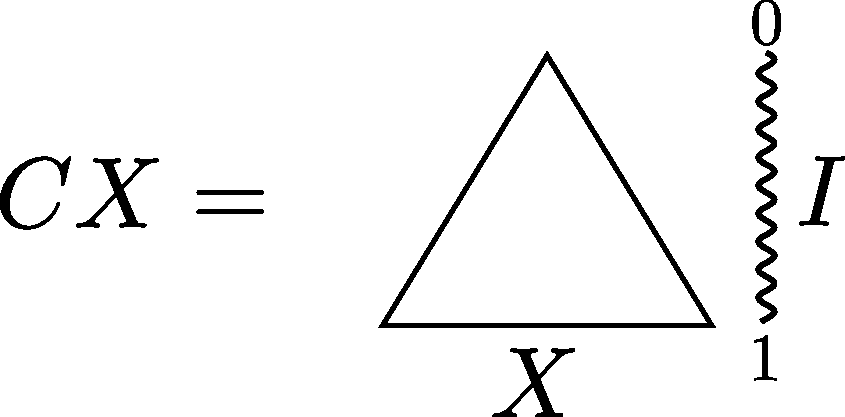
\includegraphics[width=0.2\textwidth]{figures/fig3.pdf}
%\caption{\small Diagram of the cone on $X$.}
%\end{wrapfigure}
\textbf{The Hopf construction is treated so much better in lecture \ref{TheMapsEandHinTheEHPLES}. I should really rewrite all this to reference that lecture.}

To attack this problem, it is helpful first to think about the map $\mu$ in ridiculous generality, sort of like thinking about a bilinear form in terms of a tensor product.  Namely, consider a map $\mu: X \times Y \to Z$, and consider the cone over $X$ which is defined to be the quotient $X \times I /\{(x, 0) \sim (x', 0)\}$.  The map $\mu$ then induces a map $CX \times Y \to CZ$ by $((x, t), y) \mapsto (\mu(x, y), t)$, and similarly a map $X \times CY \to CZ$.  $X \times Y$ includes into both $CX \times Y$ and $X \times CY$ as $((x, 1), y)$ and $(x, (y, 1))$ respectively, and $Z$ includes into $CZ$ as $(z, 1)$.  Putting these together, we get a diagram
%\begin{figure}[h!]
%\centering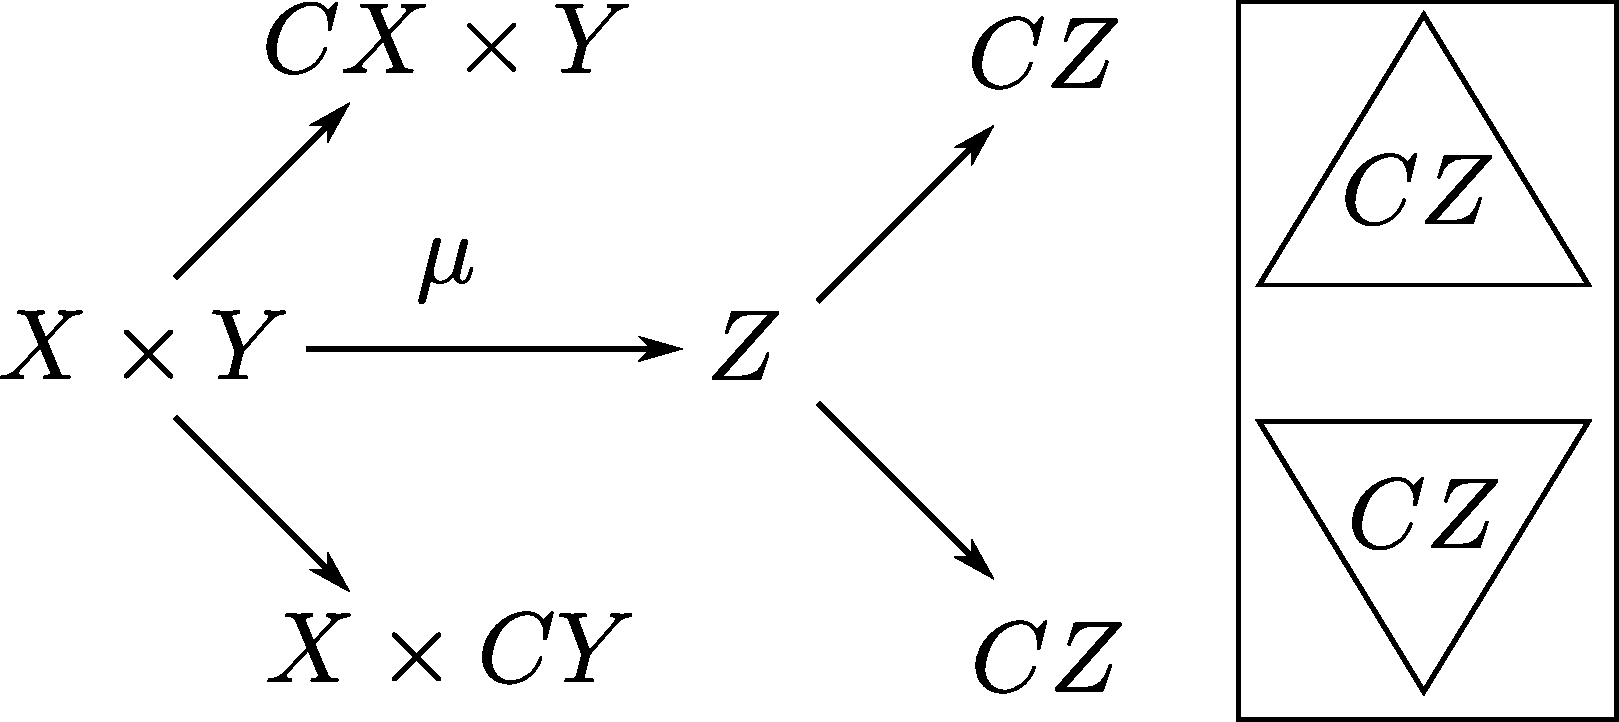
\includegraphics[width=0.35\textwidth]{figures/fig4.pdf} % %this guy is missing some arrows
%\end{figure}

The commutativity means that we can take the disjoint union of $CX \times Y$ and $X \times CY$ and identify along the copy of $X \times Y$ in each, then take two copies of $CZ$ and identify along their bases, and get a conglomerate map $H(\mu): X \ast Y \to \Suspend Z$, where $\ast$ denotes join and $\Suspend$ denotes suspension.
That is, the diagram above constitutes a map between two diagrams of shape $\bullet\leftarrow\bullet\rightarrow\bullet$, which induces a map $H(\mu)$ between their colimits (pushouts).
This process is called the ``Hopf construction'' for $\mu$, hence the name $H(\mu)$.



We note two facts about the join: first, $S^{p-1} \ast S^{q-1} = S^{p + q - 1}$, which follows from the more general statement that $X \ast Y = \Suspend(X \sprod Y)$ for reasonable $X$ and $Y$, e.g., CW-complexes.  In the case of an $H$-space, $H(\mu)$ can be written as a map $X \ast X \to \Suspend X$, and if $X = S^{n-1}$, this is a map $S^{2n-1} \to S^n$, i.e., a homotopy class of a the $n$-sphere, something to be prized and studied. % use \pi_n notation here
}

\begin{wrapfigure}{r}{0.3\textwidth}
\centering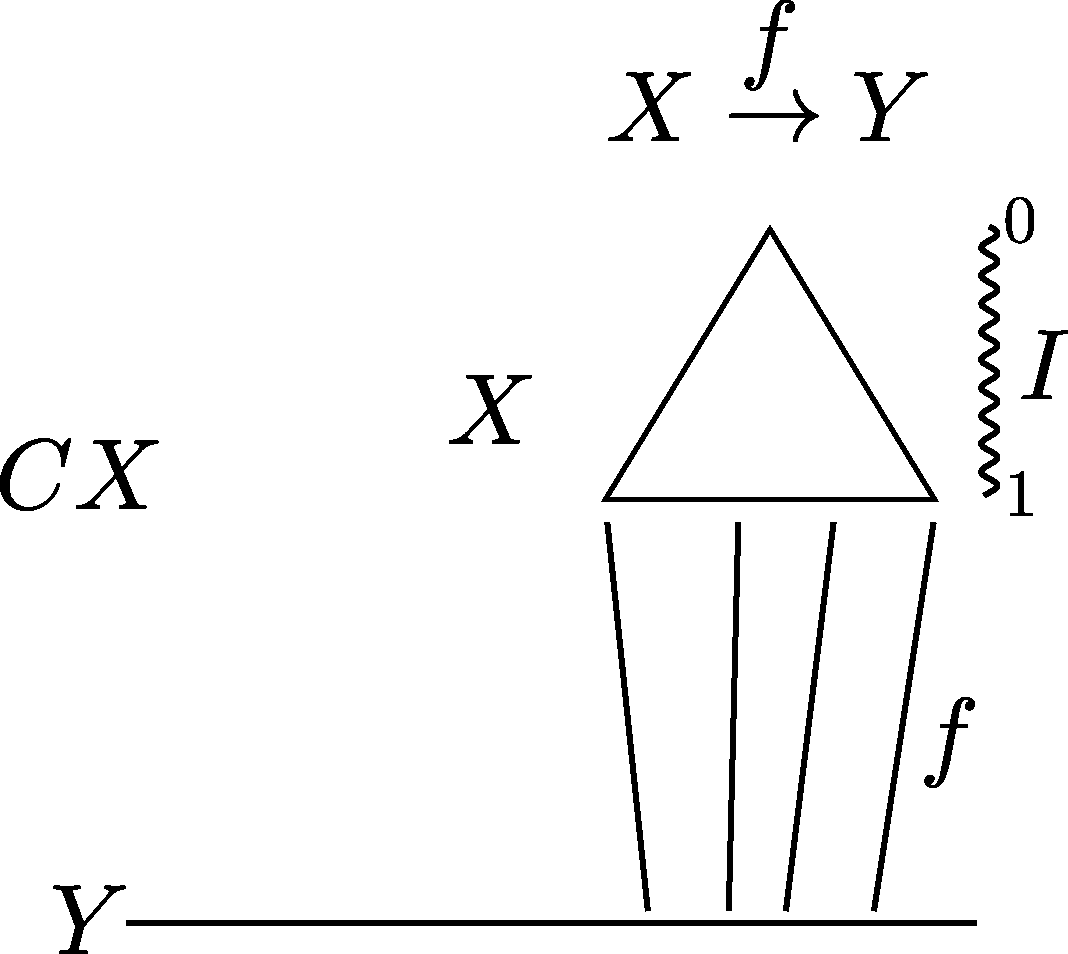
\includegraphics[width=0.23\textwidth]{figures/fig5.pdf}
\caption{\small Diagram of the mapping cone on $f$.}
\end{wrapfigure} % in the following paragraph, try to talk about the general case and the specific case of the cone on a Hopf map separately.  also, the definiiton of the cone is missing brackets and Y, CX change order.  'really means', 'is obstained by'
There is a duality in homotopy between maps and objects; namely, to every map there is an associated space which contains all the information about the map, called the mapping cone.  Associated to a map $f: X \to Y$, we build $C_f = Y \amalg CX / (x, 1) \sim f(x)$.  $Y$ includes into $C_f$ as its base, so one has a ``cofiber sequence'' $X \to Y \to C_f$.  Applying this to the map $H(\mu): S^{2n-1} \to S^n$, the mapping cone really means just attaching a $2n$-cell to $S^n$ via the map $H(\mu)$, so we get $S^{2n-1} \xrightarrow{H(\mu)} S^n  \to S^n \cup_{H(\mu)} e^{2n}$.  Now, (assuming $n > 1$) the cohomology is given by
\[
H^*(S^n \cup_{H(\mu)} e^{2n}) =
\begin{cases}
\Zbb & \hbox{generated by $y$ in degree $2n$,} \\
\Zbb & \hbox{generated by $x$ in degree $n$,} \\
\Zbb & \hbox{generated by $1$ in degree $0$.}
\end{cases}
\]
Using the cup product, $x^2 = \alpha y$ for some $\alpha \in \Zbb$, where for now $\alpha$ is well-defined only up to sign.  This coefficient $\alpha$ is called the Hopf invariant of $\mu$.  We make the unsubstantiated\footnote{Unsubstantiated for now --- see lecture \ref{TheMapsEandHinTheEHPLES}.} claim that $\alpha = \pm 1$ for $H(\mu)$ whenever $\mu$ is an $H$-space multiplication on the $(n-1)$-sphere.  As examples, we have
\begin{ctikzcd}[row sep=tiny]
S^3 \rar & S^2 \rar & S^2 \cup e^4 = \CP^2, \\
S^7 \rar & S^4 \rar & S^4 \cup e^8 = \HP^2, \\
S^{15} \rar & S^8 \rar & S^8 \cup e^{16} = \OP^2,
\end{ctikzcd}
where the last is called the ``Cayley projective plane.''  (Note that nonassociativity of Cayley multiplication implies that there are no other Cayley projective spaces.) % what does this mean?  no higher OP^n, right?  not that there's anything after O...?

So now the question is: for what spheres is there an element of $\pi_{2n-1} S^n$ of Hopf invariant $1$?
\begin{thm}[Adams] % hopf invariant was only defined for n > 1 :)
If $\pi_{2n-1} (S^n)$ contains an element of Hopf invariant $1$, then $n = 1$, $2$, $4$, or $8$.
\end{thm}
For the time being, take a step back and recall the action $O(n) \times S^{n-1} \to S^{n-1}$.  Any $\alpha \in \pi_k (O(n))$ (not necessarily from a section) induces a map $S^k \times S^{n-1} \to O(n) \times S^{n-1} \to S^{n-1}$.  Doing the Hopf construction here induces a map $S^{k+n} \to S^n$, i.e., we get what turns out to be a homomorphism $J: \pi_k (O(n)) \to \pi_{n+k} (S^n)$ called the ``$J$-homomorphism.''  For $k < n$, $\pi_k (O(n))$ are known by Bott periodicity, hence there is much interest in the image of $J$.  Note that for $k < n$, $n + k > 2k$, and this is the so-called ``stable range'' where things often seem to work better; one then thinks of $J$ as a map $\pi_* (O) \to \Pi_*$.  The Adams conjectures are concerned with the image of this $J$. % should stability really be mentioned here?

% >>>
\fi
\BoxedNote{\Bullet $S^{n-1}$ has $k-1$ linearly independent vector fields iff $V_{n,k}\downarrow S^{n-1}$ has a section.

\Bullet The largest $k$ such that there is such a section is $\rho(n)$, where we write $n=\textup{odd}\cdot 2^{\nu}$, $\nu=4b+c$ for $0\leq c\leq3$, and $\rho=8b+2^c$.

\Bullet The Hopf construction takes a map $\mu:X\times Y\to Z$ to a map $H(\mu):X*Y\to\Sigma Z$.

\Bullet If $S^{n-1}$ is parallelizable, it can be made into an H-space (essentially, apply the Hopf construction to a section $V_{n,n}\downarrow S^{n-1}$). This happens when $n=1,2,4,8$ by the previous point.

\Bullet (It is claimed that) if $\mu$ is an $H$-space multiplication on $S^{n-1}$, $H(\mu)$ has Hopf invariant one. We'll see later that this  can only happen when $n=1,2,4,8$.

\Bullet The $J$-homomorphism $J:\pi_k(O(n))\to \pi_{n+k}(S^n)$ sends $\alpha:S^k\to O(n)$ to the Hopf construction applied to $S^k\times S^{n-1}\xrightarrow{\alpha\times1}O(n)\times S^{n+1}\to S^{n-1}$.
}
\section{Clifford algebras} % <<<
\label{CliffordAlgebras}
\ifx\OutputCliffordAlgebras\undefined\else

In this lecture we will see how many vector fields on spheres we can construct using linear algebra; we will use Clifford algebras.  For more information, see for example the book by Strang.

For $k \ge 0$, the Clifford algebra $C_k$ is the associative $\Rbb$-algebra generated by $e_1, \ldots, e_k$, subject to relations
\begin{align*}
e_i e_j + e_j e_i & = 0 \hbox{\;for $i \ne j$}, \\
e_i^2 & = -1.
\end{align*}
For example,
\begin{align*}
C_0 & = \Rbb, \\
C_1 & \cong \Cbb, \hbox{ note: you can identify $e_1$ with $i$ or $-i$, so the iso.\ is not canonical} \\
C_2 & \cong \Hbb, \hbox{ with, say, $e_1 \mapsto i$, $e_2 \mapsto j$, $e_1 e_2 \mapsto k$}
\end{align*}
Note that the relations specify that we can give a basis for $C_k$ as the set of words $\{e_{i_1} \cdots e_{i_m} \mid m \ge 0, i_1 < \cdots < i_m\}$ made up of ordered nonrepeating sequences of the generators.  So $\dim C_k = 2^k$.  Note also that the collection $G_k = \{ \pm e_{i_1} \cdots e_{i_m} \mid m \ge 0, i_1 < \cdots < i_m\}$ is a multiplicative subgroup of $C_k$.  Also, $C_k$ comes equipped with an antiautomorphism $C_k \to C_k$, defined on generators by $\bar e_i = -e_i$, and extended to $C_k$ as an antiautomorphism.  It is an anti-involution in the sense that $\overline{xy} = \ybar\xbar$.

Before describing the $C_k$ further, let's look at how they can be used to construct vector fields on spheres.  One gets there by finding representations of $C_k$. Suppose $V$ is an $n$-dimensional vector space with a $C_k$-module structure $C_k \otimes_\Rbb V \to V$.  $V$ is then a representation of $C_k$.  Next choose any inner product on $V$.  By averaging over the action of $G_k$ we can construct a $G_k$-invariant inner product $(-, -)$.  Let $S(V)$ denote the unit sphere of $V$, and note that points of $S(V)$ are invariant under action by the $e_i$.  We claim
\begin{thm}
For $x \in S(V)$, $\{e_1 x, \ldots, e_k x\}$ defines an orthonormal $k$-frame on $S(V) \cong S^{n-1}$.
\end{thm}
\begin{proof}
First, $(x, e_i x) = (e_i x, e_i e_i x) = -(e_i x, x) = -(x, e_i x)$, so $(x, e_i x) = 0$ and $e_i x$ is tangent to $S(V)$ at $x$.  Second, if $i \ne j$, we have $(e_i x, e_j x) = (e_i e_j e_i x, e_i e_j e_j x) = (-e_i^2 e_j x, e_i e_j^2 x) = (e_j x, (-e_i x)) = -(e_i x, e_j x)$.  So $(e_i x, e_j x) = 0$, and $e_i x$ and $e_j x$ are orthogonal.
\end{proof}
In particular, one way to find an orthonormal $k$-frame on $S^{n-1}$ is to find an $n$-dimensional $C_k$-module. To find as may orthonormal vector fields as possible of $S^{n-1}$ we should find the largest $k$ such that $C_k$ admits an $n$-dimensional module.
Thus we will search for low-dimensional representations of $C_k$.

From now on, write $C^+_k$ for $C_k$. As we identify more of the algebras $C^+_k$, we build up the following table. The column $C^+_k$ identifies the isomorphism type of $C^+_k$ in terms of better known $\Rbb$-algebras. Here, if $A$ is an $\Rbb$-algebra, $A(r)$ is used as a shorthand for the algebra of $r\times r$ matrices with entries in $A$. For each $k$, we write $a_k$ for the minimal dimension of a nonzero $C^+_k$-module (see lemma \ref{MinRepsOfAlgs}). Note that $\Hbb^2$ acts on $\Hbb\cong\Rbb^4$ via $(a,b)c=ac\overline{b}$, and similarly, $\Rbb(8)^2$ acts on $\Rbb^8$ via $(M,N)v=MvN^\textup{tr}$. The last column will be identified later.
%Michael: Should say here `of a minimal C_k-module, as shown in lemma \ref{}....' or something
\[\begin{array}{c|ccccc} % this table might go better after the calculations.  most the definition of phi over to the right as a log of a_k.  use less ridiculous notation for matrix rings.  why are these the minimum dimensions of the representations??
k& C^+_k& a_k & \varphi_k = \log_2 a_k &C^-_k \\\hline
0 & \Rbb & 1 & 0 & \Rbb \\
1 & \Cbb & 2 & 1 & \Rbb^2 \\
2 & \Hbb & 4 & 2 & \Rbb(2) \\
3 & \Hbb^2 & 4 & 2 & \Cbb(2) \\
4 & \Hbb(2) & 8 & 3 & \Hbb(2) \\
5 & \Cbb(4) & 8 & 3 & \Hbb(2)^2 \\
6 & \Rbb(8) & 8 & 3 & \Hbb(4) \\
7 & \Rbb(8)^2 & 8 & 3 & \Cbb(8) \\
8 & \Rbb(16) & 16 & 4 & \Rbb(16).
\end{array}\] % the multiplication in the product of two algebras is component-wise -- wouldn't hurt to mention this
To identify the algebras $C_k^+$ it is useful to introduce a Clifford algebra associated to a different bilinear form. Let $C_k^-$ be the associative $\Rbb$-algebra generated by $e_1, \ldots, e_k$, subject to relations $e_ie_j+e_je_i=0$ (for $i\neq j)$ and $e_i^2=1$. For the same reasons as $C_k$ (which from now on we call $C_k^+$), $C_k^-$ is $2^k$-dimensional.

So what are the $C_k^-$?  $C_1^-$ has $1$ generator, whose square is $1$.  So $C_1^- \cong \Rbb^2$, with $e_1 \mapsto (1, -1)$ (or $(-1, 1)$).  $C_2^- \cong \Rbb(2)$ is the algebra of $(2 \times 2)$-matrices over $\Rbb$.  The isomorphism is very noncanonical; try sending % awk
$e_1$ to reflection through $L_1$ and $e_2$ to reflection through $L_2$, where $L_1$ and $L_2$ are any lines separated by $45$ degrees.  Thus, $e_1e_2$ and $e_2e_1$ correspond to rotation by $90$ degrees, one clockwise and the other counterclockwise, depending upon the relative orientation of the lines.  This could get very tiring very quickly; fortunately that's as far as we need to go.  From now on, we use
\begin{lem}
For $k \ge 2$, $C_k^\pm \cong C_2^\pm \otimes C_{k-2}^\mp$.
\end{lem}
\begin{proof}
Again, this is highly noncanonical.  For example,
\[
e_i \mapsto
\begin{cases}
e_1 \otimes 1 & : i = 1, \\
e_2 \otimes 1 & : i = 2, \\
e_1e_2 \otimes e_{i-2} &: i > 2
\end{cases}
\]
works.  (As an exercise, complete this proof.) % TODO: Remove this exercise
\end{proof}

The remaining $C_k^\pm$ in the table can be computed in succession using this lemma, sort of like ``tying up the laces on a skate''; to do this one uses the following isomorphisms:
\begin{align*}
(\Rbb \times \Rbb) \otimes A & \cong A \times A \\
\Rbb(n) \otimes A & \cong A(n) \\
\Hbb \otimes \Cbb & \cong \Cbb(2) \\
\Rbb(m) \otimes \Rbb(n) & \cong \Rbb(mn) \\
\Hbb \otimes \Hbb & \cong \Rbb(4).
\end{align*}
From the table we can also quickly compute $C_k$ for $k > 8$ if we note the isomorphisms obtained by repeatedly applying the lemma:
\begin{align*}
C_k^+ & \cong C_2^+ \otimes C_{k-2}^- \\
& \cong C_2^+ \otimes C_2^- \otimes C^+_{k-4} \\
& \cong C_4^+ \otimes C_{k-4}^+ \\
& \cong C_4^+ \otimes (C_4^+ \otimes C_{k-8}^+) \cong C_8^+ \otimes C_{k-8}^+ \\
& \cong C_{k-8}^+(16).
\end{align*}
(Similarly, $C_k^- \cong C_{k-8}^-(16)$.)

The third column, $a_k$, corresponds to the minimal representation of the Clifford algebra $C_k^+$.  We can quickly determine this column using the following lemma:
\begin{lem}\label{MinRepsOfAlgs}
We compute the following dimensions of minimal representations of algebras:
\begin{enumerate}
\item When $A$ is a skew field, $A$ acting on itself is a minimal representation, so the minimal dimension is $1$.
\item When $A$ is a skew field and $A(n)$ is the space of $n \times n$-matrices over $A$, then $A(n)$ acting on $A^n$ is a minimal representation, so the minimal dimension is $n$.
\item When $A$ and $B$ are two algebras, then the dimension of a minimal representation for $A \otimes B$ is the product of the dimensions for minimal representations of $A$ and $B$ individually.
\end{enumerate}
\end{lem}
%Michael: Does this cover k=3,7
\begin{proof} These are easy exercises in commutative algebra. \end{proof}
The fourth column is $\varphi_k = \log_2 a_k$, where $a_k$ is the dimension of the minimal representation.  From $C_k^+ \cong C_{k-8}^+(16)$ we get that $a_{k+8} = 16 a_k$, or $\varphi_{k + 8} = \varphi_k + 4$.
% be consistent about whether phi should be a subscript or a function

Finally, we can apply this to vector fields on spheres.  There are $k$ linearly independent vector fields on $S^{a_k - 1}$; by taking $c$ copies of the vector space and using the diagonal action, there are $k$ linearly independent vector fields on $S^{ca_k - 1}$.  Now fix the dimension $n-1$ of the sphere and maximize $k$; i.e., for $S^{n-1}$, maximize $\{k\,:\,a_k | n\} = \{ k\,:\, \varphi_k \le \nu(n)\}$ (where $\nu(n)$ is the function from before).  The first few cases are:
\[\begin{array}{c|ccccccc}
\nu(n) & 0 & 1 & 2 & 3 & 4 & 5 & 6 \\
\hline
k_{max} & 0 & 1 & 3 & 7 & 8 & 9 & 11
\end{array}\]
and this is exactly $\rho(n) - 1$ from before.  So we have succeeded in constructing $\rho(n) - 1$ linearly independent vector fields on the $(n-1)$-sphere.  It turns out that this is the best we can do using linear algebra --- in fact this really is the best we can do with any tools.
\fi
\BoxedNote{
\Bullet We have constructed $k$ vector fields on $S^{n-1}$ whenever $a_k|n$, where $a_k=2^{\varphi_k}$ is the minimal dimension of a representation of $C_k$.

\Bullet We also noted that $a_k|n\iff k\leq\rho(n)-1$, and thus have constructed as many vector fields as possible.}

%>>>



\section{Building Thom spaces} % <<<
\label{BuildingThomSpaces}
\ifx\OutputBuildingThomSpaces\undefined\else
We'll now start attacking the second part of the vector field problem.  Recall that the Stiefel manifold $V_{n, k}$ of $k$-frames on $\R^n$ is given by $(n \times k)$-matrices with orthonormal columns, and projection onto the first column gives a fiber bundle $V_{n, k-1} \into V_{n, k} \onto S^{n-1}$.  The existence of a section $s$ of this bundle is equivalent to the existence of $(k-1)$ orthonormal vector fields on $S^{n-1}$.

Now we will find a consequence for the existence of such a section in the homotopy theory of $\RP^{k-1}$.  To start with, there are two important facts about $\RP^{k-1}$.  The first is the existence of a fiber bundle $\Z_2 \into S^{k-1} \onto \RP^{k-1}$ obtained by identifying antipodal points on $S^{k-1}$.  The second is the existence of the ``tautological line bundle'' $L = \{(l, x) \in \RP^{k-1} \times \R^k \mid x \in l\} \onto \RP^{k-1}$, where one thinks of $\RP^{k-1}$ as the space of lines through the origin on $\R^k$.  These two constructions are, of course, related: there is a metric on $L$ induced by the metric in $\R^k$; taking the vectors of length $1$ in each fiber gives $S(L)$, the unit sphere bundle of $L$, and $S(L) \cong S^{k-1}$.

On the other hand, we can recover $L$ as $S^{k-1} \times_{\Z_2} \R$; this is an example of the ``Borel construction.'' % define what a twisted product is.  it would a lso be useful to talk about why the Borel construction is useful; you can sort of always move to your favorite spot in the fiber.  this definition should also match use of the borel construction in lecture 6
More generally, if $F$ is any space with a $\Z_2$ action, we get a bundle with fiber $F$ by taking $F \into S^{k-1} \times_{\Z_2} F \onto \RP^{k-1}$.  What follows from a section $s$ of $V_{n, k} \onto S^{n-1}$ is:
\begin{lem}
If there is a section $s$, then there is a bundle map $\hat s$ over $\RP^{k-1}$ of the form
%\begin{diagram}[height=2em]
%\hat{s}: S(n \epsilon) & \rTo & S(n L) \\
%\uEqualto & & \uEqualto \\
%\RP^{k-1} \times S^{n-1} & & S^{k-1} \times_{\Z_2} S^{n-1},
%\end{diagram}
\[\xymatrix@R=.6cm{
\makebox[0cm][r]{$\RP^{k-1} \times S^{n-1}=$\ }S(n \epsilon)\ar[r]^{\hat s}\ar[d]&
S(nL)\makebox[0cm][l]{\ $=S^{k-1} \times_{\Z_2} S^{n-1}$}\ar[d]\\
\RP^{k-1}\ar@{=}[r]&\RP^{k-1}
}\]
which acts as the identity on the fiber over the point $\pm e_1$, which we take as the basepoint in $\RP^{k-1}$.
(Here $\epsilon$ is the trivial bundle of dimension $1$ and $\Z$ acts on bundles by direct sum.)
\end{lem}
\begin{proof}
Define $\hat s: \R^k \times S^{n-1} \to \R^k \times S^{n-1}$ by $\hat s(x, v) = (x, s(v) x)$.  It is straightforward to see $|s(v) x| = 1$ if $|x| = 1$, so $\hat s$ maps $S^{k-1} \times S^{n-1} \to S^{k-1} \times S^{n-1}$.  Quotienting the target by $\Z_2$, we have \[\hat s(-x, v) = (-x, -s(v)x) = (x, s(v) x) = \hat{s}(x, v),\] so it descends to a quotient on the source: $\hat{s}: \RP^{k-1} \times S^{n-1} = S(n \epsilon) \to S^{k-1} \times_{\Z_2} S^{n-1} = S(nL)$.  Finally, $s(v)e_1 = v$ (as $s$ is a section), so $\hat{s}(e_1, v) = (e_1, v)$.
\end{proof}
One point worth mentioning here is that $\hat s$ could have been defined as a map $n \epsilon \to n L$, but it would not necessarily have been linear on each fiber (as $s(v)$ is not necessarily linear), so the map would not have been in a strict sense a map of vector bundles.  Previously, we constructed such sections $s$ using Clifford algebras, and in that case $s$ was in fact linear.  In some sense, then, the problem is to find out whether you can get more vector fields by modifying them in some clever way.

The fact that $\hat s$ induces the identity over $\pm e_1$ means that $\hat s$ induces a homotopy equivalence on each fiber.  Explicitly, for any open and connected $U \subseteq \RP^{k-1}$ such that $nL|_U$ is trivial and such that $\hat s_b$ is a homotopy equivalence for some $b \in U$, it follows that $\hat s$ induces a map $U \to \Hom(S^{n-1}, S^{n-1})$.  As $U$ is connected, it lands entirely in one path-connected component of $\Hom(S^{n-1}, S^{n-1})$, and hence the map on fibers is a homotopy equivalence.

We have two bundles $E$ and $E'$ over a base $B$ and a bundle map $f: E \to E'$ which induces a homotopy equivalence on each fiber.  What we really want is a map $g$ going back so that $fg$ and $gf$ are homotopic through bundle maps to the respective identity maps;  $f$ is then called a ``fiber homotopy equivalence.''  Fortunately there is a very nice theorem due to Dold:
\begin{thm}[Dold]\label{LemmaOfDold}
Suppose $E$ and $E'$ are fibrations over $B$ with a bundle map $f$ inducing a homotopy equivalence on each fiber.  If $E$ and $E'$ have the homotopy type of CW complexes and $B$ is connected, then $f$ has a fiber homotopy inverse.
\end{thm}
\begin{proof}
See \cite{James}.
\end{proof}
In this context, the lemma gives
\begin{cor}
If $V_{n, k} \onto S^{n-1}$ sections, then $S(nL) \onto \RP^{k-1}$ is fiber homotopy trivial.
\end{cor}
Ultimately we will show the result of Adams that this implies that $k \le \rho(n) - 1$, i.e., that $a_k$ divides $n$.


\begin{wrapfigure}{r}{0.3\textwidth}
\centering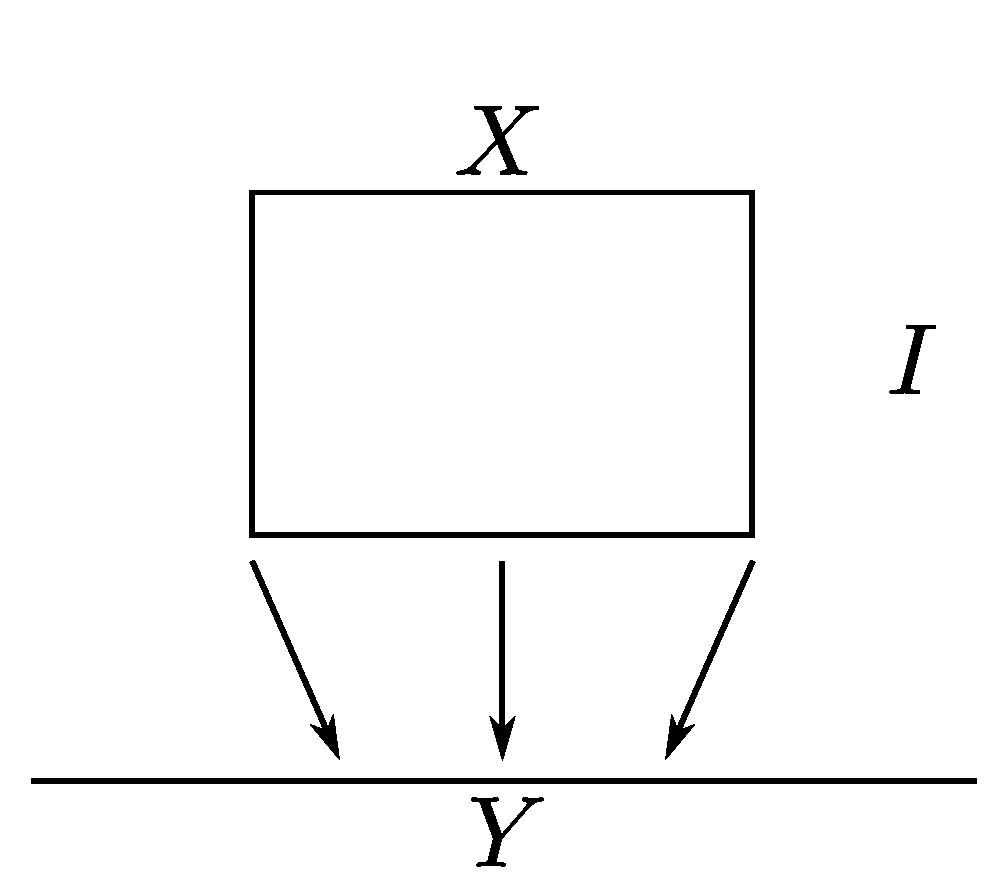
\includegraphics[width=0.2\textwidth]{figures/fig7.pdf}
\caption{\small Diagram of the mapping cylinder of $f$.}
\end{wrapfigure} % define the mapping cylinder, since we defined the mapping cone earlier.  in fact, this figure belongs to such a discussion, and should be treated separately.  why is this important that we can do it for "any" sphere bundle??
Next we look at the consequences of the discussion so far in terms of Thom spaces.  Suppose $E \onto B$ is a vector bundle with a metric, so there's a nice sphere bundle $p$ defined as the composite $S(E) \into E \onto B$.  In order to understand the map $p$, we could look again at the mapping cone $Cp = B \cup_p C_{S(E)}$ of $p$.

Given a map $f:X\to Y$, we can construct the cone $Cf$ in two stages, leaving pinching the cone for the ``second stage''. The intermediate space $Mf=X\times I\cup_f Y$ is called the ``mapping cylinder,'' and it is homotopy equivalent to $Y$.  Moreover there is a nice inclusion $X \into Mf$ which is a cofibration. Then $Cf$ is obtained by collapsing the image of $X$ in $Mf$.

In fact, it doesn't matter how you replace the space $Y$ with a homotopy equivalent space: as long as the map $f$ is replaced by a cofibration, collapsing out its image we obtain a space homotopic to the mapping cone.
%This is true, right?

Now in the case of $p: S(E) \onto B$, the mapping cone is called the Thom space, $T(E)$.
One can think of the mapping cylinder $p:S(E)\to B$ as being the disk bundle $D(E)$ of vectors of length less than or equal to $1$; the Thom space is then the quotient space $D(E) / S(E)$.

As a passing (but important) remark, the fibers of these two bundles over a basepoint $b \in B$ are $S^{n-1} \subset S(E)$ and $D^n \subset D(E)$, and pinching the former out of the latter gives an $S^n$ in $T(E)$.  So if $B$ is connected and $E$ is oriented, the Thom space comes with a unique, distinguished class in $\pi_n T(E)$.

\begin{wrapfigure}{r}{0.5\textwidth}
\centering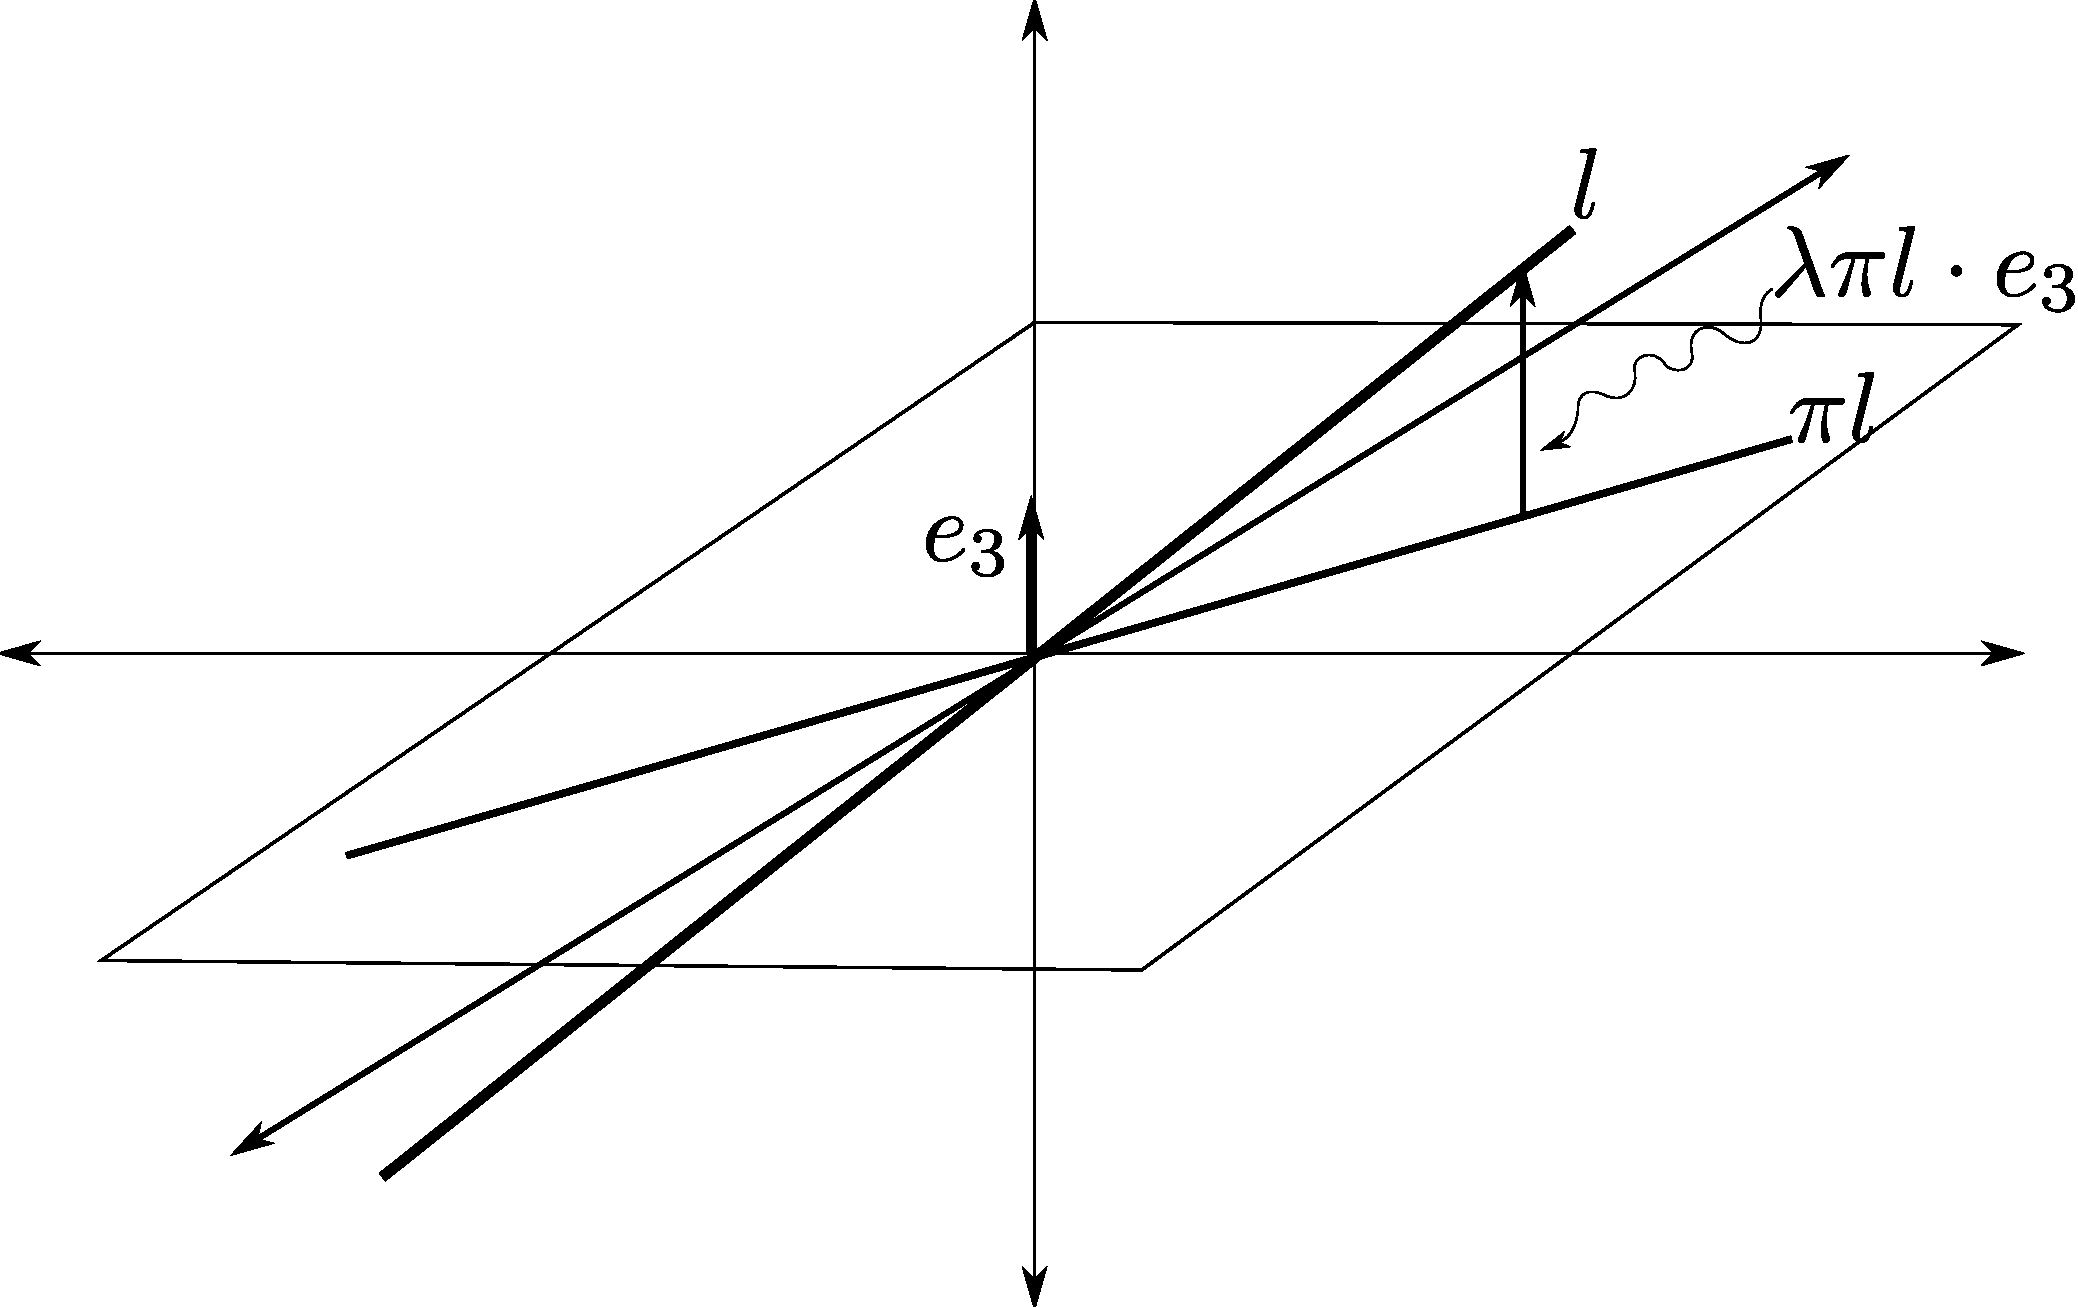
\includegraphics[width=0.4\textwidth]{figures/fig8.pdf}
\caption{\small Recovering $l$.}
\end{wrapfigure} % how can we make it clear that the lambda_i depend upon the point l in RP^k-1?
Next, we return to $nL$, the bundle over $\RP^{k-1}$, where $L$ is the tautological line bundle.  We claim that this bundle is the normal bundle $\nu$ of the inclusion $\RP^{k-1} \into \RP^{n+k-1}$ induced by the inclusion $\R^k \into \R^{n+k}$.  To wit, pick a point $l \in \RP^{n+k-1}$ parametrized as $l(t)$, a line in $\R^{n+k}$.  Let $\pi l \in \RP^{k-1}$ be the projection of this line to a line in $\R^k$.  We can recover the line $l$ in $\R^{k+n} \cong \R^k \times \R \times \cdots \times \R$ by $l(t) = (\pi l(t), \lambda_1(\pi l(t)), \ldots, \lambda_n(\pi l(t)))$ for some functions $\lambda_i$ dependent upon $l$.  Clearly $\lambda_i(rv) = r \lambda_i(v)$, so $\lambda_i \in L^*$.  Hence the normal bundle can be identified with $nL^*$.  Since $nL$ comes equipped with a metric, this gives an isomorphism of the normal bundle $\nu$ with $nL$.

% what?
But there's even more structure around.  \ConfusedBox{ Remarking that $\RP^{n+k-1}$ forms a vector bundle of rank $n$ over $\RP^{k-1}$ and using the inclusion of the open unit ball in $\R^n$ to $\R^n$, \textsc{(what does this mean?)}} one can construct a map from $D(\nu)$ to $\RP^{n+k-1}$ such that $S(\nu)$ maps to $\RP^{n-1}$ and which is a relative homeomorphism $(D(\nu), S(\nu)) \to (\RP^{n+k-1}, \RP^{n-1})$.\footnote{One candidate for the map $D(\nu)\to\RP^{n+k-1}$ can be specified as follows. View $D(\nu)$ as $D(nL)$, where $nL\subset \RP^{k-1}\times (\R^k)^n$ inherits its metric from the standard Euclidean metric on $(\R^k)^n$. Then a point of $D(\nu)$ is an $n+1$-tuple $(\R\{z\},r_1z,r_2z,\ldots,r_nz)$, where $z\in R^k$ has length one, $\|r\|^2=\sum r_i^2\leq1$. The map sends this point to $(z,r_1,r_2,\ldots,r_n)$.}
It follows that the Thom space of $nL$ is $T(nL)\simeq\RP^{n+k-1}/\RP^{n-1}$. In particular, if $nL$ is being fiber homotopy trivial, then $T(n\epsilon) \simeq T(nL) \cong \RP^{n+k-1}/\RP^{n-1}$.
%
% sends $([z], r_1z, \ldots, r_nz)\in D(\nu)\subseteq \R P^{k-1}\times (\R^k)^n$, where $[z]=\R z\in\RP^{k-1}$ for $z\in\R^k$ to }

% >>>
\fi
\BoxedNote{
%\Bullet Lemma of Dold: if a map of fibrations (with the homotopy type of CW-complexes) over a connected base $B$ is a homotopy equivalence on each fiber, it has a fiber homotopy inverse.
%
%\Bullet Lemma of Dold: maps of nice fibrations over the same connected base restricting to a homotopy equivalence on each fiber have fiber homotopy inverses.
%
\Bullet Dold: suppose $f:E_1\to E_2$ is a map of fibrations $E_i\downarrow B$, the $E_i$ have the homotopy type of a CW-complex, and $B$ is connected. Then if $f$ restricts to a homotopy equivalence on each fiber, it has a fiber homotopy inverse.

\Bullet $nL\onto \R P^{k-1}$ is the normal bundle of the inclusion into $\R P^{n+k-1}$.

\Bullet If $V_{n, k} \onto S^{n-1}$ sections, then $S(nL)\onto \R P^{k-1}$ is fiber homotopy trivial.

\Bullet $T(nL)\simeq \RP^{n+k-1}_n:=\R P^{n+k-1}/\R P^{n-1}$ ``stunted projective space'' (any $n,k$).

\Bullet In particular, if $S^{n-1}$ admits $k-1$ vector fields, $T(n\epsilon)\simeq T(nL)\simeq \R P^{n+k-1}_n$.
}
\section{Facts about Thom spaces} % <<<
\label{FactsAboutThomSpaces}
\ifx\OutputFactsAboutThomSpaces\undefined\else
We'll now look at Thom spaces in more detail, and in particular in relation to some other standard constructions on fiber bundles.  First of all, we have a product: given two bundles $F \to E \to B$ and $F' \to E' \to B'$, we can build a bundle $F \times F' \to E \times E' \to B \times B'$.  Now if $B = B'$, you can pull this bundle back along the diagonal map to a bundle $F \times F' \to E \times_B E' \to B$, called the ``fiberwise product.''  If $E$ and $E'$ are vector bundles, then $E \times_B E'$ is called the ``Whitney sum,'' denoted $E \oplus E'$.

\begin{wrapfigure}{r}{0.33\textwidth} % maybe it would be better to give a drawing more reflective of the construction
\centering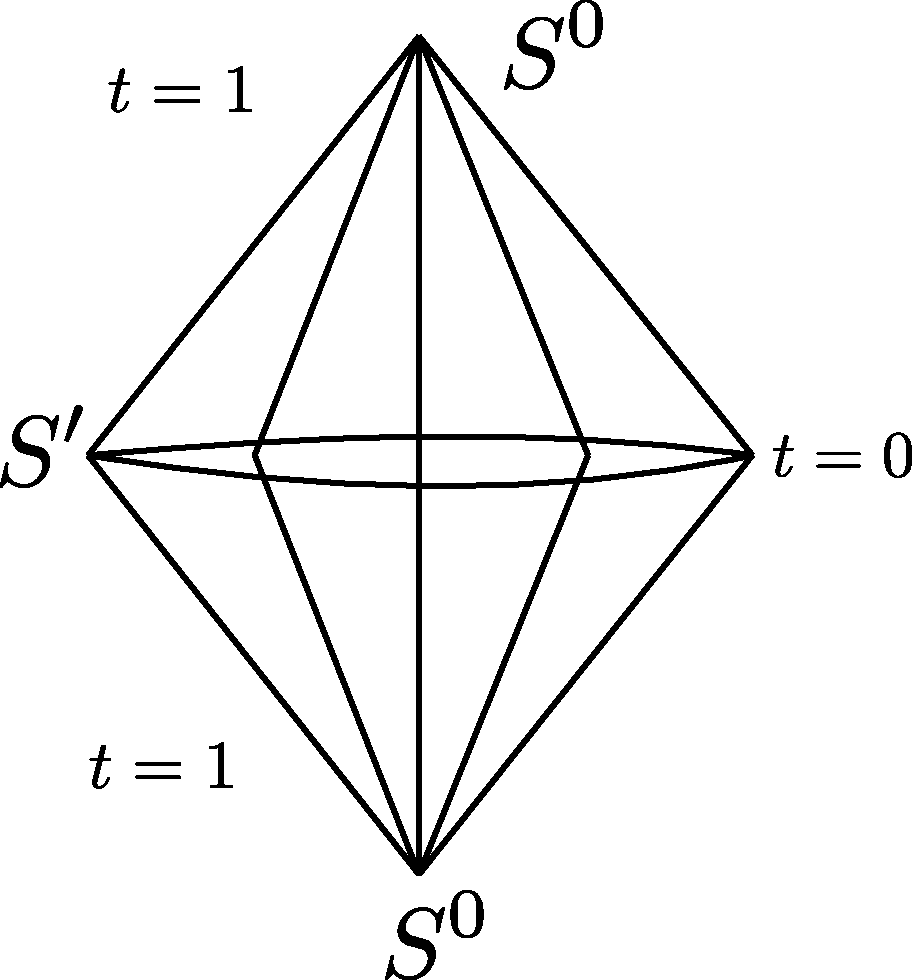
\includegraphics[width=0.3\textwidth]{figures/fig9.pdf}
\caption{\small A diagram of $S^0 \ast S^1$.}
\end{wrapfigure}
If $E$ and $E'$ are sphere bundles, this construction isn't very satisfying, because a sphere cross a sphere isn't another sphere.  However, the join of two spheres is another sphere.  Here's another way of looking at the join\footnote{As an aside, we define $X \ast \emptyset = \emptyset \ast X = X$.} (we will return to the join often, and try as often as possible to give different definitions of it!):
\[
X \ast Y = \frac{X \times I \times Y}{(x, 1, y) \sim (x, 1, y'), (x, 0, y) \sim (x', 0, y)}.
\]
Now we define a fiberwise join by doing this on each fiber to get a bundle $F \ast F' \to E\mathop{\widehat\ast}E' \to B \times B'$, where \[E\mathop{\widehat\ast}E' = \frac{E \times I \times E'}{\substack{\hbox{$(x, 1, y) \sim (x, 1, y')$ if $p'y = p'y'$}, \\ \hbox{$(x, 0, y) \sim (x', 0, y)$ if $px = px'$.}}}\]  One can check that this construction yields something locally trivial.  The fiberwise join for sphere bundles is related to the fiberwise product of vector bundles: if $V$ and $W$ are vector bundles, then $S(V \times W) = SV \,\widehat \ast \,SW$.  Moreover, if $B = B'$ we can once again pull back by the diagonal map on $B$, and we get $SV \ast_B SW = S(V \oplus W)$.

In the case that $Y = \ptspace$, $X \ast Y = CX$ is the cone over $X$.  Applying this in the fiberwise join, we transport a bundle $F \to E \to B$ to a bundle $CF \to C_B E \to B$, where $C_BE:=E\mathop{\widehat\ast}B$.  Applying this to a sphere bundle $E \to B$ gives a disk bundle $C_B E \to B$, and it's easy to check that if $V$ is a vector bundle, then $D(V) = C_B S(V)$, so we have a way of recovering the disk bundle from the sphere bundle.

Now back to Thom spaces.  Recall that if $E \onto B$ is a sphere bundle, its Thom space is $T(E) = C_B E / E$, and if the fiber over the basepoint of $B$ in $E$ is $S^{n-1}$, then $CS^{n-1} = D^n \subset C_B E$, which becomes an $S^n \subset T(E)$.  The Thom space comes equipped with a canonical basepoint which is the image of $E$, which has been crushed to a point.  If $V \onto B$ is a vector bundle, then $T(V)$ is defined to be $T(S(V))$, and also $T(0) = \pt{B}:=B \amalg \ptspace$.\footnote{By convention, $0$ denotes the rank zero vector bundle.  In this case $S(0) = E = \emptyset$, and we write $T(\emptyset) = B / \emptyset = B \amalg \ptspace$ also by convention.  This is done so that the smash product identity below works.}

To understand this better, let's look at the trivial sphere bundle $B \times S^{n-1} \to B$.  Here, we have $T(B \times S^{n-1}) = B \times D^n / B \times S^{n-1}$.  Now as $S^n\cong D^n/S^{n-1}$, it follows that:
\[T(B \times S^{n-1}) = \frac{B \times D^n}{B \times S^{n-1}} \cong \frac{B \times S^n}{B \times \ptspace} \cong \pt{B} \sprod S^n = \Suspend^n(\pt{B}),\]
and so the Thom space of a bundle can be thought of as a twisted sort of suspension.

Here's an important fact: $T(E\, \widehat \ast\, E') = T(E) \sprod T(E')$, where $\sprod$ is the smash product of pointed spaces.  A rough proof in the special case that $E = SV$ and $E' = SW$ for vector bundles $V\downarrow B$ and $V'\downarrow B'$ is:
%\begin{align*}
%TV \sprod TW & = T(S(V)) \sprod T(S(W)) \\ %A bit wordy
%& = \frac{DV}{SV} \sprod \frac{DW}{SW} \\
%& = \frac{\frac{DV}{SV} \times \frac{DW}{SW}}{\frac{DV}{SV} \wsum \frac{DW}{SW}} \\
%& = \frac{DV \times DW}{(SV \times DW) \cup (DV \times SW)} \\
%& \cong \frac{D(V \times W)}{S(V \times W)} \\
%& = T(S(V \times W)) = T(E\,\widehat \ast\, E').
%\end{align*}
\[TV \sprod TW = \frac{DV \times DW}{(SV \times DW) \cup (DV \times SW)}\cong \frac{D(V \times W)}{S(V \times W)}= T(S(V \times W)) = T(E\,\widehat \ast\, E').\]
In the special case that $E' \to B'$ is $\R^n \to \ptspace$, we get that $T(V \oplus n \epsilon) = T(V) \sprod S^n = \Suspend^n T(V)$.

Note that if $V$, $W$ are vector bundles over $B$, it is \textbf{not} the case that $T(V\oplus W)=T(V)\wedge T(W)$. However, we have a pullback diagram (drawn on the left) which induces a map of Thom spaces (drawn on the right). This map commutes with the inclusion of the copies of $S^{n+m}$ (where $\dim_*V=n$ and $\dim_*W=m$):
\[\xymatrix{
V\oplus W\ar[d]\ar[r]&V\times W\ar[d]\\
B\ar[r]^\Delta&B\times B
}\qquad\qquad
\xymatrix{
T(V\oplus W\downarrow B)\ar[r]&T(V\times W\downarrow B\times B)
\ar@{=}[r]&T(V\downarrow B)\wedge T(W\downarrow B)\\
&S^{n+m}\ar[ul]\ar[u]\ar@{=}[r]&S^n\wedge S^{m}\ar[u]
}\]

The Thom space is useful for deciding whether a fiber bundle is trivial.  To this end, we observe that if $E$ and $E'$ are fiber homotopy equivalent $S^{n-1}$-bundles, then $T(E) \simeq T(E')$ relative to the copies of $S^n$ over the basepoint in $B$.
\begin{lem}\label{LemOnFHTrivialisations}
Suppose that $E \to B$ is an $S^{n-1}$-bundle. Then fiber homotopy equivalences $h:E\to B\times S^{n-1}$ are in bijection with maps $f:E\to S^{n-1}$ whose restriction to each fiber is a homotopy equivalence. Moreover, if any such maps exist (i.e.\ if $E\to B$ is fiber homotopy trivial), then each map $f$ induces a ``coreduction'':
\[\xymatrix@R=.6cm{
T(E)\ar[r]&S^n\\
S^n\ar[u]\ar[ur]_\simeq
}\]
\end{lem}
\begin{proof}
Write $\pi_2:B\times S^{n-1}\to S^{n-1}$ for the second projection. Then (by the universal property of the product), fiber maps $h:E\to B\times S^{n-1}$ are in bijective correspondence with maps $f:E\to S^{n-1}$, via $h\mapsto \pi_2h$. Now we note that fiber homotopy equivalences $h$ correspond exactly to maps $f$ inducing a homotopy equivalence on each fiber. If such a map $f$ exists, it can be thought of as a bundle map
\[\xymatrix@R=.4cm{
E\ar[r]^f\ar[d]& S^{n-1}\ar[d]\\
B\ar[r]&\ast
}\raisebox{-.4cm}{\textup{\qquad which induces a map on Thom spaces:\qquad}}
\xymatrix@R=.4cm{
T(E)\ar[r]&S^n=\makebox[0cm][l]{$T(S^{n-1}\downarrow*)$}\\
S^n\ar[u]\ar[ur]_\simeq
}\qquad\qquad\]
and the homotopy equivalence of $f$ restricted to each fiber implies that the map $S^n\to S^n$ is a homotopy equivalence.
\end{proof}
\noindent Now the game is to find obstructions to the splitting off of this $n$-sphere, which is in fact the bottom-dimensional cell in $T(E)$.

Of course, what we really want is an obstruction to a fiber homotopy equivalence between $nL$ and $n \epsilon$, and a coreduction of $T(E)$ need not imply that $E$ itself is fiber homotopy trivial.  To find out what we \emph{do} get from a coreduction of $T(E)$, we look at another construction of the Thom space (and think of the name Bott when thinking about $T(E)$ in this way).  We build $T(E)$ in two steps:
\begin{enumerate}
\item Collapse to a sphere in each fiber $F$, i.e., take $D(F) / S(F)$ in each fiber of $E \to B$.  This gives a sphere bundle, along with a ``section at $\infty$'' given by the image of $S(F)$ in each fiber.
\item Collapse the section at $\infty$ to a point.
\end{enumerate}
This exhibits $T(E)$ as the sphere bundle $S(E \oplus \epsilon)$ with the $1$-section of $\epsilon$, which is homeomorphic to $B$, smashed to a point, so $T(E) = S(E \oplus \epsilon) / B$, after identifying $B$ with that section. % the difference here is that you're adding a point at infinity to each fiber, then collecting all the points at infinity together.

Now the fiber in $S(E \oplus \epsilon)$ is the same as the $S^n$ sitting in $T(E)$, so with this construction a coreduction for $T(E)$ gives
\begin{diagram}[height=2em]
S(E \oplus \varepsilon) & \rTo & T(E) & \rTo & S^n \\
& \luTo & \uTo & \ruTo_\simeq \\
& & S^n.
\end{diagram} % in fact, in all of these diagrams, it would be nice if S^n weren't sitting in the base's position.
If the base $B$ is connected, then from Dold's theorem (\ref{LemmaOfDold}) it follows that $E \oplus \epsilon$ is fiber homotopy trivial. % this sentence is completely vacuous when B is a CW-complex, so who cares about Dold's theorem
So a coreduction of $T(E)$ implies that $S(E \oplus \epsilon)$ is fiber homotopy trivial.

This is a process of stabilization: the lesson of this discussion is that we have to play back and forth with various processes of this kind: suspend the Thom space, sum in a trivial bundle, and so on.  These connections yield the natural role of $K$-theory. % maybe we could include a diagram exemplifying that the Thom space of eps (+) E is the same as the suspension of the Thom space of E
\fi
\BoxedNote{
\Bullet The fiberwise join of fiber bundles was constructed. Given $E\downarrow B$, performing the join with $B\downarrow B$ yields a bundle $C_BE$, the fiberwise cone. This recoves the disk bundle from a sphere bundle, and gives another definition of the Thom space of a sphere bundle $E$: $C_BE/E$.

\Bullet $T(E\, \widehat \ast\, E') = T(E) \sprod T(E')$ for bundles $E\downarrow B$ and $E'\downarrow B'$.

\Bullet $T(V\times W\downarrow B\times B')=T(V)\sprod T(W)$, where $V\times W$ is the exterior direct sum of vector bundles $V\downarrow B$ and $W\downarrow B'$.

\Bullet If $V,W$ are vector bundles over $B$, then $T(V\oplus W\downarrow B)\to T(V\times W\downarrow B\times B)$ is not a homotopy equivalence, but is compatible with the various inclusions of spheres over basepoints.

\Bullet If $E,E'$ are f.h.eq.\ $S^{n-1}$-bundles then $T(E)\simeq T(E')$ relative to the copies of $S^n$ over the basepoint.

\Bullet A fiber homotopy trivialisation of an $S^{n-1}$-bundle $E\downarrow B$ induces a \emph{coreduction}: maps $S^n\to T(E)\to S^n$ with composite $\simeq\textup{id}$, splitting off the bottom cell.

\Bullet If a coreduction of $T(E)$ exists then $S(E\oplus\epsilon)$ is fiber homotopy trivial.
}
% >>>
\section{Building \texorpdfstring{$K$}{K}-theory and \texorpdfstring{$J$}{J}-theory} % <<<
\label{BuildingKandJtheory}
\ifx\OutputBuildingKandJtheory\undefined\else
Now a few introductory words on $K$-theory: let $X$ be a pointed %finite complex (it is at least necessary that $X$ be a
compact Hausdorff space.  Let $\Vect(X)$ be the set of isomorphism classes of vector bundles over $X$.\footnote{Why is $\Vect(X)$ a set?}  The Whitney sum gives a monoid structure to $\Vect(X)$, with zero given by the $0$-dimensional vector bundle.  Now one applies the ``Grothendieck construction,'' which simply means to add formal inverses, making a group; explicitly, we form equivalence classes of pairs $(V,W)$ under the equivalence relation in which $(V, W) \sim (V', W')$ iff $E + V + W' \cong V' + W + E$ for some vector bundle $E$.  Here, $(V, W)$ is supposed to represent the formal difference ``$V - W$''.  This is an abelian group, called $KO(X)$.

Now it may not seem that $KO(X)$ has topological significance, but in view of the last lecture, it quickly becomes apparent that it does.  For if $V \oplus n\epsilon \cong W \oplus n\epsilon$ for some $n$ ($V$ and $W$ are said to be ``stably isomorphic''), then the classes $[V]$ and $[W]$ are equal in $KO(X)$.  Moreover, as $X$ is a compact Hausdorff space, it goes both ways.  Suppose $[V] = [W]$, so $V + E \cong W + E$ for some $E$.  Over a compact Hausdorff space, any vector bundle $E$ is a subbundle of a sufficiently big trivial bundle
\begin{diagram}[height=2em]
E & \rInto & X \times \R^N \\
\dTo & \ldTo \\
X,
\end{diagram}
as we shall soon see.  By choosing a metric on $\R^N$, we get an orthogonal complement $F \to X$ such that $E \oplus F$ is trivial.  Then $V \oplus E \oplus F \cong W \oplus E \oplus F$, so $V$ and $W$ are stably isomorphic!

%Throughout, let $X$ be a pointed compact Hausdorff space.  Recall that $KO(X)$ was defined to be the abelian group given by the Grothendieck construction on the monoid $\Vect(X)$.
If $f: X \to Y$ is a map and $E \to Y$ is a vector bundle, then $E$ pulls back by $f$ to a vector bundle $f^* E \to X$, so we have a map $f^*: KO(Y) \to KO(X)$.  Pullbacks by homotopic maps induce isomorphic bundles, so $f \simeq g$ implies $f^* = g^*$.  Hence $KO$ is a contravariant functor $ \mathit{ho}\mathsf{Top} \to \mathsf{AbGrp}$. % it would be smart to come up with a notation for vector bundles, like f^* E downarrow X

Now the canonical maps $\ptspace \to X \to \ptspace$ induce maps $KO(\ptspace) \stackrel{\eta}{\to} KO(X) \stackrel{\epsilon} \to KO(\ptspace)$.  It is clear that $KO(\ptspace) = \Z$, that $\im \eta$ consists of trivial bundles, and that $\epsilon(V,W)=\dim_*(V)-\dim_*(W)$ takes the difference of the dimensions of the fibers over the basepoint.  Reduced $KO$-theory is defined in terms of these maps.  There are two equivalent definitions: % point out that this sequence is induced by the triangle pt --> X --> pt, with the composite a homotopy equivalence.
\[ % this isn't defined piecewise, so we are we using this bracket notation?
\widetilde{KO}(X) = \begin{cases}
\ker \epsilon & \hbox{: virtual vector bundles, i.e., formal differences $V - W$ with the same rank, or} \\
\coker \eta & \hbox{: i.e.,\ $\Vect(X)/\approx$, where $V\approx W$ iff $V \oplus m \epsilon \cong W \oplus n \epsilon$ for some $m,n\geq0$}.
%\coker \eta & \hbox{: $[V] = [W]$ if and only if $V \oplus m \epsilon \cong W \oplus n \epsilon$}. % aaron finds this line confusing, so we should change it
\end{cases}\]
The description here of $\coker\eta$ is correct as any equivalence class in $KO(X)$ contains a pair of the form $(V,n\epsilon)$. To obtain such a pair in the class of $(V',W')$, find $W''$ such that $W'+W''$ is trivial, as above, and then $(V',W')\sim (V'+W'',W'+W'')$.
Notice that $\coker\eta$ is the just the monoid $\Vect(X)$ taken modulo the equivalence relation generated by $V\approx V\oplus\epsilon$, which turns out to be a group, by the above argument.

Similarly, any equivalence class in $\ker\epsilon$ contains a pair of the form $(V,n\epsilon)$ where $n=\dim_*(V)$. We often denote this equivalence class $[V]-n$.


Next we'll see, as advertised, how to embed a vector bundle into a high-dimensional trivial bundle.  Suppose $p: E \to X$ is a rank $n$ vector bundle.  Because $X$ is compact Hausdorff, it has a finite open cover $U_1, \ldots, U_k$ that trivializes $E$.  That is, there are homeomorphisms $f_i$ with
\begin{diagram}[height=2em]
E|_{U_i} & \rTo^{f_i} & U_i \times \R^n \\
\dTo<p & \ldTo>{\pi} \\
U_i,
\end{diagram}
such that the triangle commutes and $f_i$ is linear on each fiber.  Let $\phi_1, \ldots, \phi_k$ be a partition of unity subordinate to the cover $\{U_i\}$, and define maps $g_1, \ldots, g_k: E \to \R^n$ by
\[
g_i =
\begin{cases}
E|_{U_i} \stackrel{f_i}{\to} U \times \R^n \stackrel{(x, v) \mapsto \phi_i(x) \cdot v}{\longrightarrow} \R^n, \\
\hbox{$0$ on $E$ away from $U_i$}.
\end{cases}\]
The $g_i$ give a linear embedding $f: E \to X \times (\R^n)^k$ defined by $f(e) = (p(e), g_1(e), \ldots, g_k(e))$.

This map in fact gives more: to each $x \in X$ we associate the $n$-dimensional subspace $f(E_x)$ of $\R^N$ with $N = nk$.  This induces a classifying map $h$ from $X$ to the Grassmannian of $n$-planes in $\R^N$.  Over $G_{N, n}$ is the tautological $n$-plane bundle $E_{N, n}$, \[E_{N, n} = \{(v, p) \mid p \in G_{N, n}, \hbox{$v$ a member of the subspace associated to $p$}\}\] and we have in fact expressed $E \to X$ as the pullback of the tautological bundle along $h$.  From this point of view it is clear that the choice of $N$ is somewhat arbitrary; there are obvious inclusions $G_{N, n} \subseteq G_{N+1, n} \subseteq G_{N+2, n} \subseteq \cdots$, and $E$ can be induced from the tautological bundle over $G_{N, n}$ for any sufficiently large $N$.  Thus we have a classifying space $BO(n) = \bigcup_N G_{N, n}$, and it represents rank $n$ vector bundles over $X$ via $\Vect_n(X) \stackrel{\cong}{\to} [X, BO(n)]$.

What happens when we descend to $KO(X)$?  First, the equivalence $V \sim V \oplus \epsilon$ gives us $\widetilde{KO}$, % is Grothendieck(Vect) / this relation the same as Vect / this relation? Yes - Now discussed above.
so we get $\widetilde{KO}$ by identifying an element of $[X, BO(n)]$ with an element of $[X, BO(n+1)]$ when all it does is add a trivial bundle.  Now if $EO(n)$ is the tautological $n$-plane bundle over $BO(n)$, % should this be called the canonical O(n)-bundle?  should we warn the reader we're going to mix these things together using the Borel construction?
then $EO(n) \oplus \epsilon$ is an $(n+1)$-plane bundle, and there is a classifying map $BO(n)\to BO(n+1)$ for this bundle. We obtain a sequence:
\begin{diagram}[height=2em]
%EO(n) \oplus \epsilon & & EO(n+1) \oplus \epsilon \\
%\dTo & & \dTo \\
\cdots & \rTo & BO(n) & \rTo & BO(n+1) & \rTo & \cdots
\end{diagram}
of classifying maps whose colimit $\bigcup_n BO(n)$ is called $BO$, and $\widetilde{KO}(X) = [X, BO]$.\footnote{%
This argument can be summarised as follows: $\widetilde{KO}(X)=\textup{colim}[X,BO(n)]$, which equals $[X,\textup{colim}BO(n)]$ as $X$ is compact.
}
Finally, $KO$ remembers dimension, so $KO(X) = [X, \Z \times BO]$. % where Z keeps track of the virtual dimension

Now let's talk about $J$-theory.  If $V$ and $W$ are vector bundles over $X$, then we write $V \sim_J W$ if $S(V \oplus n \epsilon)$ and $S(W \oplus n \epsilon)$ are fiber homotopy equivalent for some $n\geq0$. This idea is analogous to $K$ on the level of sphere bundles, and defines an additive equivalence relation on $KO(X)$. $J(X)$ is defined to be the quotient of $KO(X)$ given by this relation, and $\widetilde J(X)$ the image of $\widetilde{KO}(X)$. % there should be an equation attached to this last sentence
Now from the Clifford algebra story we know that over $\RP^k$ the tautological line bundle $L$ has $a_k L \cong a_k \epsilon$. % this a_k was defined in day 2, remind the reader
Considering the class $[L] - 1 \in \widetilde{KO}(\RP^k)$, this means $a_k([L] - 1) = 0$. In fact: % say early on that we're going to identify n eps with n.
\begin{thm}[Adams]\label{AdamsKORPn}
$\widetilde{KO}(\RP^k)=\Z/a_k\Z$ generated by $[L]-1$.
$\widetilde{KO}(\RP^k) \stackrel{\cong}{\onto} \widetilde J(\RP^k)$ is an isomorphism.
\end{thm}
In other words, there are no other trivializations, and so % remind the reader that we were talking about coreductions earlier
\begin{cor}
If $S(nL) \to \RP^k$ is fiber homotopy trivial, then $a_k$ divides $n$. In particular, there are at most $\rho(n) - 1$ vector fields on $S^{n-1}$. % this should have a proof attached, reminding the reader of the chain of implications
\end{cor}
\begin{proof}
Suppose that $S(nL)$ is fiber homotopy trivial. Then $n[L]$ equals $n[\epsilon]$ in $\widetilde J(\R P^k)$, and so $n([L]-1)=0$ in $\widetilde{KO}(\RP^k)$, implying that $a_k|n$. This demonstrates the first claim.

Now we saw in lecture \ref{CliffordAlgebras} that $a_k|n$ iff $k\leq \rho(n)-1$. We saw in lecture \ref{BuildingThomSpaces} that if $V_{n, k+1} \onto S^{n-1}$ sections, then $S(nL)\onto \R P^{k}$ is fiber homotopy trivial. Thus, if $V_{n, k+1} \onto S^{n-1}$ sections, we must have $k\leq\rho(n)-1$.
\end{proof}
One of the things we get out of this theorem is that $\widetilde{KO}(\RP^k)$ is finite. In general: % really i think this and the previous immediate theorems should be moved down below Atiyah's theorem
\begin{thm}[Atiyah]
If $X$ is a finite connected complex, then $\widetilde J(X)$ is finite.
\end{thm}
\begin{proof}(Sketch, anyway.)
A vector bundle over $X$ is classified by a map $X \to BO(n)$.  Similarly a sphere bundle should have a similar classifying procedure.  In general, the structure group would have to be taken to be $\textup{Homeo}(S^{n-1})$, % use the same formula as below, but without the basepoints
but since we are only concerned with fiber homotopy equivalences we should be able to use the monoid $G_n$ of homotopy self-equivalences of $S^{n-1}$.  Such a classifying procedure exists; call the corresponding space $BG_n$.  Now there is a natural inclusion $O_n \into G_n$, and hence maps
\begin{diagram}[width=2em,height=2em]
BO(n) & \rTo & BG_n \\
\dTo & & \dTo \\
BO & \rTo & BG.
\end{diagram}
We then make two claims: $\widetilde J(X)$ is the image of $[X, BO] \to [X, BG]$, and $[X, BG]$ is finite.  We prove this last part cell-by-cell, so what we really need to show is that $\pi_i(BG_n)$ is finite for $i$ much smaller than $n$.  Since $X$ is finite, $[X, BG] \simeq [X, BG_n]$ for some $n$ sufficiently larger than the top-dimensional cell of $X$, so this is enough.  There is a fibration $G_n \to EG_n \to BG_n$, and hence $\pi_i BG_n \cong \pi_{i-1} G_n$.  We are then left with showing that $\pi_i G_n$ is finite (again, for $i$ must smaller than $n$).  Now an element of $G_n$ is a map $S^{n-1} \to S^{n-1}$; by evaluating at the basepoint in $S^{n-1}$ we get a map $G_n \to S^{n-1}$.  This is a fibration whose fiber is homotopy equivalent to $\Loops^{n-1}_{\pm 1}S^{n-1} := \{f: (S^{n-1}, s_0) \to (S^{n-1}, s_0) : \deg f = \pm 1\} \subseteq \textup{Maps}(S^{n-1}, S^{n-1})$.  For $i$ much smaller than $n$, $\pi_i G_n \cong \pi_i(\Loops^{n-1}_\pm S^{n-1})$ and $\pi_i(\Loops^{n-1}_\pm S^{n-1}) \subset \pi_i(\Loops^{n-1} S^{n-1}) = \pi_{i+n-1} S^{n-1} = \Pi_i$, which is known to be finite by a theorem of Serre.
\end{proof}
\fi

\BoxedNote{
\Bullet For any bundle $E$ on a compact Hausdorff space there is a bundle $E'$ such that $E\oplus E'$ is trivial.

\Bullet$\widetilde {KO}(X)$ can be viewed as (i) $\Vect(X)/\approx$, where $\approx$ is generated by $V\approx X\oplus\epsilon$, or (ii) as equivalence classes of virtual vector bundles $V-W$, where $\dim V=\dim W$.

\Bullet Adams: $\widetilde{KO}(\RP^k)=\Z/a_k\Z$ generated by $[L]-1$, and the canonical epimorphism $\widetilde{KO}(\RP^k)\to\widetilde{J}(\RP^k)$ is an isomorphism, solving the vector field problem.

\Bullet Atiyah: $\widetilde J(X)$ is finite for $X$ a finite connected complex.
}

% >>>



\section{Geometry and the Steenrod squares} % <<<
\label{GeometryAndTheSteenrodSquares}
\ifx\OutputGeometryAndTheSteenrodSquares\undefined\else
Today begins a several days blitz on Steenrod operations, from a somewhat geometric point of view.
%  To begin, remember that reduced ordinary cohomology is representable:
%\[
%\Htwee^q(X; \pi) = [X, K(\pi, q)].
%.\]
%\qquad\textup{For example:}\qquad
%\[
%\Htwee^q (S^n;\pi) = \pi_n (K(\pi, q)) = \begin{cases}\pi & q = n, \\ 0 & q \ne n.\end{cases}
%\]

Fix from the beginning a subgroup $\pi$ of the symmetric group $\Sigma_n$ (we will mostly be concerned with the case $\pi = \Z_2=\Sigma_2$).
Consider the space $E\pi$, a contractible CW-complex with a free $\pi$-action, and the orbit space $B\pi=E\pi/\pi$. Fix a choice of $E\pi$ and a point $e\in E\pi$, and let $b\in B\pi$ be its image.

For example, if $\pi = \Z_2$, then $\pi$ acts antipodally on $S^{n-1}$.  $S^{n-1}$ is not contractible, but its image is contractible in $S^n$; that is, the inclusion $S^{n-1} \into S^n$ is null-homotopic.  So the direct limit of the inclusions $S^{n-1} \subset S^n \subset \cdots = \bigcup_n S^n = S^\infty$ is contractible and has a free $\pi$-action.  The orbit space $E\pi/\pi = B\pi$ is clearly seen to be $\RP^\infty$.


A basepoint $\ast$ in a space $X$ gives a lot more than you might think at first.  It induces, for example, a filtration of the $n$-fold product $X^n$, by defining:
\[
F_k X^n = \{(x_1, \ldots, x_k)\in X^n \mid \hbox{at most $k$ of the $x_i$ differ from $*$}\}
,\text{ so that:}\]
\begin{ctikzcd}[sep = tiny]
F_0X^n \dar[equal]& \subseteq & F_1X^n \dar[equal]& \subseteq & \cdots & \subseteq & F_{n-1}X^n \dar[equal]& \subseteq & F_nX^n\dar[equal]\\
\ptspace & & \bigvee_{i=1}^n X & & & & \hbox{``Fat wedge''} & & X^n
\end{ctikzcd}
% The equal signs look really ugly to me, but the internet says it's a pdf viewer problem...

There is an action of $\pi$ on $X^n$ permuting the factors, and this action preserves the filtration.

Okay, so here's the key construction: on the universal $\pi$-bundle $E\pi \to B\pi$, use the Borel construction to mix in $X^n$; we thus obtain a locally trivial bundle over $B\pi$ with fiber $X^n$:
\begin{ctikzcd}
X^n\rar & E\pi \times_\pi X^n \dar\\
&B\pi
\end{ctikzcd}
(Recall that $\pi$ acts diagonally on $E\pi \times X^n$, and $E\pi \times_\pi X^n$ is obtained as the quotient space of this action.)  This construction is called the ``$\pi$-extended power of $X$.''

Now the fact that the $\pi$-action on $X^n$ respects the filtration means that we have a sub-bundle
\begin{ctikzcd}[column sep = tiny]
E\pi \times_\pi F_{n-1}X^n\dar & \subseteq & E\pi \times_\pi X^n\dar \\
B\pi \ar[rr,equal] & & B\pi
\end{ctikzcd}
We want to pinch this subbundle to a point.  First, as $X^n / F_{n-1} X^n\cong X^{(n)}:=X\sprod\cdots\sprod X$, the $n$-fold smash product of $X$ with itself, we have:
\[
\frac{E\pi \times_\pi X^n}{E\pi \times_\pi F_{n-1} X^n} = \frac{E\pi \times_\pi X^{(n)}}{E\pi \times_\pi \ptspace}
.\]
This is almost the smash product, but $E\pi$ doesn't have a basepoint. Instead:%  But we can just add one in and then take the smash product, and this has no effect --- so
\[
\frac{E\pi \times_\pi X^n}{E\pi \times_\pi F_{n-1}X^n} = E\pi_+ \sprod_\pi X^{(n)}
,\]
where the symbol $\sprod_\pi$ means to take the orbit space of the diagonal action on $E\pi_+ \sprod X^{(n)},$ and $E\pi_+$ refers to $E\pi$ with a disjoint basepoint added.  This is called the ``$\pi$-adic construction'' on $X$ (for lack, really, of a better name), and will be written $D_\pi(X)$.

Now a map $f:X\to Y$ induces a map $D_\pi(X)\to D_\pi(Y)$, making $D_\pi$ into a functor.
Moreover, there is a map $i_X:X^{(n)}\to D_\pi(X)$ defined simply by $x\mapsto (e,x)$. Note that we can also describe $i_X$ in terms of the map $\ibar_X:X^n\to E\pi\times_\pi X^n$ defined by $x\mapsto(e,x)$. As $F_{n-1}X^n$ is mapped into $E\pi\times_\pi F_{n-1}X^n$, the map $\ibar_X$ descends to the quotient, and gives $i_X$:
\[i_X:X^{(n)}=\frac{X^n}{F_{n-1}X^n}\to \frac{E\pi \times_\pi X^n}{E\pi \times_\pi F_{n-1}X^n} = E\pi_+ \sprod_\pi X^{(n)}.\]

The maps $i_X$ constitute a natural transformation of functors $(\textup{---})^{(n)}\to D_\pi$, in the sense that for every $f:X\to Y$, there is a commuting diagram:
\begin{ctikzcd}
X^{(n)}\rar["f^{\sprod n}"]\dar["i_X"'] & Y^{(n)}\dar["i_Y"]\\
D_\pi X\rar["D_\pi f"] & D_\pi Y
\end{ctikzcd}

For clarity, we list a number of functors and natural transformations that will soon be in use:
\begin{itemize}
\item $D_\pi(\DASH):\mathsf{Top}_*\to\mathsf{Top}_*$ as described above.
\item $(\textup{---})^{(n)}:\mathsf{Top}_*\to\mathsf{Top}_*$, the $n$-fold smash product.
\item $\Htwee^*(\DASH):=\Htwee^*(\textup{---};\F_p):\mathsf{Top}_*\to\mathsf{ComGrAlg}_{\F_p}$, ordinary reduced cohomology with coefficients in the field of $p$ elements, for some chosen prime $p$. This takes values in the category of (graded)-commutative graded $\F_p$-algebras.
\item $i_\DASH:(\DASH)^{(n)}\to D_\pi(\DASH)$, the natural transformation described above.
\item $(\DASH)^{\sprod n}:\Htwee^r(\textup{---};\F_p)\to\Htwee^{nr}((\DASH)^{(n)};\F_p)$, the $n$-fold smash power of a cohomology class.
\end{itemize}



The space $D_\pi Z$ is of some concern; first we want to know its cohomology.
\begin{lem}\label{lemaboutpiadic}
Suppose that $\Htwee^i (Z) = 0$ for $i < q$, where coefficients are taken in a field $\F$, and that $\Htwee^q (Z)$ is a finite dimensional $\F$-vector space.  Then,
\[\Htwee^i(D_\pi Z)=
\begin{cases}0;&\textup{if }i<nq;\\(\Htwee^q(Z)^{\otimes n})^\pi;&\textup{if }i=nq.%;\\???;&\textup{if }i>nq
\end{cases}
\]
Moreover, $i_Z^*:\Htwee^{nq}(D_\pi Z)\to \Htwee^{np}(Z^{(n)})$ is the inclusion of the $\pi$-invariants $(\Htwee^q(Z)^{\otimes n})^\pi\subset\Htwee^q(Z)^{\otimes n}$. Here, the tensor power is taken over $\F$, and $\pi$ acts thereupon by permuting factors.
\end{lem}
\begin{proof}
%One could produce a CW-complex for $D_\pi Z$ having no cells of dimension less than $nq$. No, one cannot! What if $Z$ is a $K(Z/3,d)$ and the field is $Z/2$? Then $H^*(Z;Z/2)=0$, but there's plenty of cells.
We have a map (drawn with dotted arrows) of bundle-subbundle pairs:
\begin{ctikzcd}[sep=1.2em]
F_{n-1}Z^n\ar[dd]\ar[rd]\ar[rr, dashed] && F_{n-1}Z^n\ar[dd]\ar[rd]\\
& Z^n\ar[rr,dashed,crossing over] && \ar[dd]Z^n\\
F_{n-1}Z^n\ar[dd]\ar[rd]\ar[rr,end anchor={[xshift=-0.7em]},dashed] && \mathclapph{F_{n-1}Z^n}{\hskip1.2em E\pi\mathop{\times}\nolimits_\pi F_{n-1}Z^n}\ar[dd]\ar[rd]\\
& Z^n\ar[from=uu,crossing over]\ar[rr,end anchor={[xshift=-1.3em]}, dashed,crossing over] && \mathclapph{Z^n}{E\pi\times_\pi Z^n}\ar[dd]\\
 \{b\}\ar[rr,dashed]\ar[rd,equal] && B\pi\ar[rd,equal]\\
& \{b\}\ar[from=uu,crossing over]\ar[rr,dashed] && B\pi
\end{ctikzcd}

Now the map $Z^{(n)}=\frac{Z^n}{F_{n-1}Z^n}\longrightarrow\frac{E\pi \times_\pi Z^n}{E\pi \times_\pi F_{n-1}Z^n} = D_\pi Z$ induced by this diagram is exactly $i_Z$, so we can study $i^*_Z$ using the associated morphism of relative Serre spectral sequences.

The relative Serre spectral sequence for the pair on the left has untwisted coefficients:
\[
_LE_2^{s,t} = H^s(*; H^t(Z^n, F_{n-1} Z^n)) \Rightarrow \Htwee^{s+t}(Z^{(n)})
.\]
Now $B \pi$ is not simply connected (it is in fact a $K(\pi,1)$), so the second relative Serre spectral sequence will require twisted coefficients:
\[
_RE_2^{s,t} = H^s(B\pi; \{H^t(Z^n, F_{n-1} Z^n)\}) \Rightarrow \Htwee^{s+t}(D_\pi Z)
.\]
Now $H^*(Z^n, F_{n-1} Z^n) \cong \Htwee^* (Z^{(n)}) \cong \Htwee^*(Z)^{\otimes n}$, and this last isomorphism is equivariant with respect to permutations, a fact that is not trivial (and likely to be false with other cohomology theories).  It follows that in both spectral sequences, everything is zero below the horizontal line at height $nq$ in the $E_2$ term. That is $E_2^{s,t}=0$ for $t<nq$.  So, % why?
\[
\Htwee^{nq}(D_\pi Z) ={_RE_2^{0,nq}}= H^0(B\pi; \{\Htwee^q(Z)^{\otimes n}\}) = (\Htwee^q(Z)^{\otimes n})^\pi.\]
Moreover, the map $i^*_Z:\Htwee^{nq}(D_\pi Z)\to \Htwee^{nq}(Z^{(n)})$ coincides with the induced map $_RE_2^{0,nq}\to{_LE_2^{0,nq}}$, i.e.: % on the $E_2$ page. This is the map
\[H^0(B\pi; \{\Htwee^q(Z)^{\otimes n}\})\to H^0(*;\Htwee^q(Z)^{\otimes n}),\]
which is simply the inclusion of the $\pi$-invariants, as desired.
\end{proof}
\noindent This is the key fact that gives the Steenrod operations; all else follows more or less from it.

From here on, for all $r$, let $K_r$ denote $K(\Z_p,r)$ and $\Htwee^r(\DASH)$ denote $\Htwee^r(\textup{---};\Z_p)$, for some chosen prime $p$.  By the Hurewicz theorem and universal coefficients theorem: % rework this lecture so that we can swap out singular cohomology for something else.  this seems to be the key confusing step
\[\Htwee^i(K_q)=0\text{ \ for $i<q$, and \ }\Htwee^q(K_q)=\Z_p.\]
%%%$\Htwee^i(K_q; \Z_2)$ is zero for $i<q$ and is $\Z_2$ when $i=q$.
%\begin{align*}
%\Htwee^i(K_q; \Z_2) & = 0, \hspace{5em} i < q \\
%\Htwee^q(K_q; \Z_2) & = \Z_2,
%\end{align*}
%by the Hurewicz theorem.
So $\Htwee^{nq}(D_\pi K_q)$ is the $\pi$-invariants in $H^{nq}(K_q^{(n)})=(\Z_p)^{\otimes n}$ under the action of $\pi$ given by interchanging terms in the tensor product. However, this action is trivial.\footnote{In fact, the standard isomorphism $(\Z_p)^{\otimes n}\to\Z_p$ is $\Sigma_n$-equivariant, where we give the target the trivial action.}
% fa Moreover, as $\pi$ can only act trivially on $\Htwee^{nq} (K_q^{(n)})=\Z_p$ \textbf{(is this true if $p\neq2$, or should we just set $p=2$ already?)},
Thus, the map
\[
\Htwee^{nq} (D_\pi K_q) \xrightarrow{\ i^*\,} \Htwee^{nq} (K_q^{(n)}) % this breaks if the action of pi isn't transitive
\]
is an isomorphism.  Now $\Htwee^{nq} (K_q^{(n)})$ contains an element $\iota_q^{\sprod n}$, the $n$-fold smash power of the fundamental class $\iota_q \in \Htwee^q( K_q)$, and we have shown:
\begin{cor}
There is a unique class $P_\pi \iota_q \in \Htwee^{nq} (D_\pi K_q)$ such that $i^* P_\pi \iota_q = \iota_q^{\sprod n}$. That is, there is a unique pointed map $P_\pi\imath_q$ up to homotopy making the following diagram commute up to homotopy:
\begin{ctikzcd}
K_q^{(n)}\dar["i"]\rar["\imath_q^{\sprod n}"] & K_{nq}\\
D_\pi K_q\urar[dashed,"P_\pi\imath_q"']
\end{ctikzcd}
\end{cor}
\noindent Here, we have abused notational by conflating the naturally isomorphic sets
$\Htwee^q(X)  \longleftrightarrow [X, K_q]_\ast$ along the isomorphism % \\
$f^* \iota_q  \longleftrightarrow [f]$, where these are functors of pointed spaces $X$.
\footnote{For example: $\Htwee^q (S^n;\pi) = \pi_n (K(\pi, q)) = \begin{cases}\pi & q = n, \\ 0 & q \ne n.\end{cases}$} We will continue to freely confuse these sets.

Now let $X$ be any space with no assumptions on its cohomology, and pick $u\in\Htwee^q(X)$.%
Representing $u\in \Htwee^q(X)$ by a map $u: X \to K_q$, we have a diagram:
%n induced map $X^{(n)} \stackrel{u^{\sprod n}}{\to} K_q^{(n)} \stackrel{\iota_q^{\sprod n}}{\to} K_{nq}$, and then the diagram

\begin{cjointikzcd}[intertext,row sep = small]
\diagram
    X^{(n)}\rar["u^{\sprod n}"]\dar["i"] & K_q^{(n)}\dar["i"]\rar["\imath_q^{\sprod n}"] & K_{nq}\\
    D_\pi X\rar["D_\pi u"]& D_\pi K_q\ar[ur,dashed,"P_\pi\imath_q"']
%
\diagram
    \intertext{which induces:}
%
\diagram
    \Htwee^{nq}X^{(n)} & \Htwee^{nq}K_q^{(n)}\lar["(u^{\sprod n})^*"'] &
    \Htwee^{nq}K_{nq}\edgerlap{\ni\imath_{nq}}
    \ar[dl,dashed,"(P_\pi\imath_q)^*"]\lar["(\imath_q^{\sprod n})^*"']\\
    %
    \Htwee^{nq}D_\pi X\ar[u,"i^*"] & \Htwee^{nq}D_\pi K_q\lar["(D_\pi u)^*"']\ar[u,"i^*"',"\cong"]
\end{cjointikzcd}%
%
So we have a natural transformation $u\mapsto (D_\pi u)^* (P_\pi\imath_q)$ of functors $H^q(\textup{---};\F_p)\longrightarrow H^{nq}(D_\pi(\textup{---});\F_p)$.
As any cohomology class $u\in\Htwee^q(X)$ can be written as $u^*(\imath_q)$, this discussion proves:
\begin{lem}
There is a unique natural transformation $P_\pi:H^q(\textup{---};\F_p)\longrightarrow H^{nq}(D_\pi(\textup{---});\F_p)$ such that $i_X^*P_\pi u=u^{\sprod n}$ for all $u\in H^q(X)$. $P_\pi u$ is called the \emph{``Steenrod power''} of $u$.
\end{lem}
%\begin{diagram}
%X^{(n)} & \rTo^{u^{\sprod n}} & K_q^{(n)} & \rTo^{\iota_q^{\sprod n}} & K_{nq}\\
%\dTo<p & & \dTo>p & \ruTo_{P_\pi \iota_q} \\
%D_\pi X & \rTo^{D_\pi u^{\sprod n}} & D_\pi K_q
%\end{diagram}
%induces a (\textbf{WRONG}) diagram on cohomology
%\begin{diagram}
%\Htwee^{nq} X^{(n)} & \lTo^{(u^{\sprod n})^*} & \Htwee^{nq} K_q^{(n)} & \lTo^{(\iota_q^{\sprod n})^*} & \Htwee^{nq} K_{nq}\\
%\uTo<{p^*}>\cong & & \uTo>{p^*}<\cong & \ldTo_{(P_\pi \iota_q)^*} \\
%\Htwee^{nq} D_\pi X & \lTo^{(D_\pi u^{\sprod n})^*} & \Htwee^{nq} D_\pi K_q
%\end{diagram}
%which shows that there is a unique class $P_\pi u = P_\pi \iota_q \circ D_\pi u^{\sprod n} \in \Htwee^{nq} D_\pi X$ such that $p^* P_\pi u = \iota_q^{\sprod n} \circ u^{\sprod n}$.
Finally, the diagonal map $\Delta: X \to X^{(n)}$ is equivariant, where we let $\pi$ act trivially on the single factor $X$, and this induces
\begin{ctikzcd}[row sep=small]
E\pi_+ \sprod_\pi X \rar["\Delta"]\dar[equal] & E \pi_+ \sprod X^{(n)}\dar[equal] \\
B \pi_+ \sprod X \rar["j"'] & D_\pi X
\end{ctikzcd}
So, any $u \in \Htwee^q (X)$ gives us a class $j^* P_\pi u \in \Htwee^{nq}(B \pi_+ \sprod X)$.

The case we will develop in full is $\pi = \Z_2$, $n = 2$, and $p=2$, so we specialise to this case now, writing $P$ for $P_\pi$ (and $\Htwee^*(\DASH)$ for $\Htwee^*(\DASH;\F_2)$). In this case, $B\pi = \RP^\infty$, and $H^*( B\pi) = \Htwee^* (B\pi_+) = \Z_2[x]$ with $|x| = 1$. By the K\"unneth theorem, $\Htwee^*(B\pi_+ \sprod X) \cong H^*(B \pi) \otimes \Htwee^* (X)$, so given $u\in\Htwee^q(X)$, we can write
%\begin{align*}
%\Htwee^*(B \pi_+ \sprod X) & \cong H^*(B \pi) \otimes \Htwee^* X \\
%j^* P u & = \sum_{i=-q}^q x^{q-i} \otimes \Sq^i u,
%\text{\qquad where $\Sq^iu\in
%\end{align*}
\[j^* P u  = \sum_{i=-q}^q x^{q-i} \otimes \Sq^i u,
\qquad\text{where $\Sq^iu\in \Htwee^{q+i}(X)$.}\]
We take this to be the definition of $\Sq^i u$. We can see immediately that $\Sq^i$ is a natural transformation $\Htwee^q\to\Htwee^{q+i}$. Moreover, $\Sq^i u$ is zero when $-q\leq i<0$, since this holds in the universal case $K(\Z_2,q)$. We define $\Sq^iu$ to be zero when $i>q$.

Note that the process above can be carried out in other cohomology theories, giving similar operations.  Mostly one needs to have computed $\Htwee^*(B \pi \sprod X)$.

Now let's start finding properties of the squares.  First of all, we don't even know that they're not all zero yet. Choose $u\in \Htwee^q(X)$. There is a map $k:S^0\to B\pi_+$, where if $S^0=\{\pm1\}$, we set $k(1)=*$ and $k(-1)=b$. We have the following diagram:
\begin{cjointikzcd}[intertext,row sep=small]
\diagram
    B\pi_+ \sprod X \rar["j"] & D_\pi X\\
    S^0 \sprod X  \rar["\Delta"]\ar[u,"k\sprod 1"] & X^{(2)}\ar[u,"i"]
%
\diagram \intertext{which induces}
%
\diagram
    \sum_{i=0}^q x^{q-i} \otimes \Sq^i u  \ar[d,mapsto] & Pu \ar[d,mapsto]\lar[mapsto] \\
     u\smile u & u^{\sprod2}\lar[mapsto]
%
\diagram \intertext{on $\Htwee^{2q}(\DASH)$.}
\end{cjointikzcd}
Now $(k\sprod 1)^*: \Z_2[x]\otimes \Htwee^* (X)\to\Htwee^* (X)$ is the projection onto $\Z_2\otimes \Htwee^* (X)$. Thus $\Sq^q u = u^2$.

Next, we derive the Cartan formula, using the following map $\delta:D_\pi(X\sprod Y)\to D_\pi(X)\sprod D_\pi(Y)$:
\begin{align*}
D_\pi(X \sprod Y) = E \pi_+ \sprod_\pi (X \sprod Y)^{(2)} & \stackrel{\delta}{\to} E \pi_+ \sprod_\pi X^{(2)} \sprod E \pi_+ \sprod_\pi Y^{(2)} = D_\pi X \sprod D_\pi Y, \\
(z, (x_1, y_1), (x_2, y_2)) & \mapsto (z, (x_1, x_2), z, (y_1, y_2)).
\end{align*}
Note that the following diagram commutes:
\begin{ctikzcd}
(X \sprod Y)^{(2)}\dar["T"] \rar["i"] & D_\pi(X \sprod Y)\dar["\delta"] &\lar["j"'] B \pi_+ \sprod (X \sprod Y)\dar["\Delta_{B\pi_+}"] \\
X^{(2)} \sprod Y^{(2)} \rar["i \sprod i"] & D_\pi X \sprod D_\pi Y & \lar["j \sprod j"'] B \pi_+ \sprod X \sprod B \pi_+ \sprod Y
\end{ctikzcd}
\begin{lem}
$\delta^*(Pu \sprod Pv) = P(u \sprod v)$.
\end{lem}
\begin{proof}
We can assume $X = K(\pi, p)$, $Y = K(\pi, q)$, $u = \iota_p$, and $v = \iota_q$.  Then the lowest dimensional cohomology of $X \sprod Y$ is $\Z_2$ in dimension $(p + q)$. Thus $i:(X\sprod Y)^{(2)}\to D_\pi(X\sprod Y)$ induces a monomorphism on $H^{2(p+q)}$, by lemma \ref{lemaboutpiadic}. Now in the diagram:
\begin{cjointikzcd}[intertext,row sep = small]
\diagram
    H^{2(p+q)}((X\sprod Y)^{(2)}) & H^{2(p+q)}(D_\pi(X\sprod Y))\lar[hook,"i^*"'] \\
    H^{2(p+q)}(X^{(2)}\sprod Y^{(2)})\ar[u,"T^*"'] & H^{2(p+q)}(D_\pi X\sprod D_\pi Y)\lar["(i\sprod i)^*"']\ar[u,"\delta^*"']
%
\diagram \intertext{we know:}
%
\diagram
    (\imath_p\sprod \imath_q)^{(2)} & \lar[mapsto]  P(\imath_p\sprod\imath_q)\\
    \imath_p^{(2)}\sprod \imath_q^{(2)} \ar[u,mapsto]& \lar[mapsto]\ar[u,mapsto] P(\imath_p)\sprod P(\imath_q)
\end{cjointikzcd}
%
In particular, because $i^*$ is a monomorphism, $\delta^*(P(\imath_p)\sprod P(\imath_q))$ must equal $P(\imath_p\sprod\imath_q)$.
%  But $(\delta i)^*(P\iota_p \sprod P\iota_q) = ((i \sprod i)T)^* (\iota_p \sprod \iota_q)$ equals $(\iota_p \sprod \iota_q)^{\sprod 2}$, and $P(\iota_p \sprod \iota_q)$ is defined to be the unique class in $H^{2(p+q)} D_\pi(X \sprod Y)$ for which this holds. % we have two nonzero things living in the same dimension, where there's only one nonzero element.
\end{proof}

\begin{cor}[Cartan formula]
$\Sq^k(u \sprod v) = \sum_{i+j = k} \Sq^i u \sprod \Sq^j v$.
\end{cor}
%
\begin{proof}
Almost immediate from the construction:
\begin{align*}
\sum_k x^{p+q-k} \otimes \Sq^k(u \sprod v) & = j^* P(u \sprod v) \\
& = j^* \delta^*(Pu \sprod Pv) \\
& = \Delta_{B \pi_+}^* (j \sprod j)^*(Pu \sprod Pv) \\
& = \Delta_{B \pi_+}^*\left[\left(\sum_i x^{p-i} \otimes \Sq^i u\right) \sprod \left(\sum_j x^{q-j} \otimes \Sq^j v\right)\right] \\ % be careful about mixing smash products and tensor products.  this happened earlier too.
& = \sum_{i, j}x^{p+q-i-j} \otimes \Sq^i u \sprod \Sq^j v.\qedhere
\end{align*}
\end{proof}
\noindent
Taking $X = Y$ and using $\Delta: X \to X \sprod X$, we obtain:
\begin{cor}[Internal version]
$\Sq^k(uv) = \sum_{i+j=k} \Sq^i u \Sq^j v$.
\end{cor}
\noindent It will be convenient to define the total squaring operation $\Sq:\Htwee^*(X)\to\Htwee^*(X)$ by $ u\mapsto\sum_i \Sq^i u$. The Cartan formula states that $\Sq$ is a ring homomorphism.

\begin{lem}
If $e$ is the generator of $\Htwee^1 (S^1) = \Z_2$ then $\Sq^0 e = e$.
\end{lem}

\begin{proof}
We know that $\Sq^i e = 0$ for $i>0$ since $H^{1+i}(S^1)=0$, so $j^*(P_{\pi}e)=x\Sq^0 e \in H^*(B\pi_+ \sprod S^1)=\Z_2[x]\otimes H^*(S^1)$.  Now $D_{\pi}S^1 = S^{\infty}_+\sprod_{\pi} S^2$, where $\pi$ acts on $S^2$ by swapping the two factors.  We can decompose $S^2$ as the smash product of the diagonal, which is a $\pi$-invariant $S^1_1$, and the antidiagonal $S^1_{-1}$ where $\pi$ acts by a reflection.  Thus $D_{\pi} S^1 = S^{\infty}_+ \sprod_\pi (S^1_1 \sprod S^1_{-1}) = (S^{\infty}_+\sprod_{\pi} S^1_{-1}) \sprod S^1_1 = \Sigma \RP^{\infty}$.  Now $B\pi_+\sprod S^1=\Sigma \RP^{\infty}$ too, and $j$ sends the $S^1$ factor into the diagonal $S^1_1$ by the identity map, so $j$ is the suspension of some map $\RP^{\infty}\to\RP^{\infty}$.  This map comes from the map $S^{\infty}\to S^{\infty}\sprod S^1$ including the $S^{\infty}$ into the $S^{\infty}$ factor by the identity map.  Thus, it sends $[x_0,x_1,\ldots]\mapsto [0,x_0,x_1,\ldots]$.  Since this map is homotopic to the identity, so is $j$ and hence $j^*$ is the identity map, and so since $P_\pi e\neq 0$, neither is $j^*P_{\pi}e$, which implies that $Sq^0e\neq 0$ so the only other option is that $\Sq^0 e = e$.
\end{proof}

% >>>
\fi
\begin{SummaryNote}
\Bullet Fix $u\in\Htwee^q(X)$. We summarise
% The following diagrams summarise
the construction of $\Sq^iu\in \Htwee^{q+i}(X)$ thus:
\begin{ctikzcd}[row sep = tiny, column sep = 1em]
B\pi_+\sprod X \rar["j"] \ar[dd,equal] & D_\pi(X) \ar[dd,equal] & X^{\sprod2}\lar["i"']
&&  \Sigma x^{q-i}\otimes \Sq^iu & \lar[mapsto,"j^*"'] Pu \rar[mapsto, "i^*"] & u\sprod u\\
%
&&& \tikzintertext{on $\Htwee^{2q}$:}\\
%
E\pi_+\sprod_\pi X\rar["\Delta"]\ar[uu,equal] & E\pi_+\sprod_\pi X^{(2)}\ar[uu,equal]
&&&& u\mathrlap{{}\in \Htwee^q{X}}\ar[uu,mapsto] & \qquad
\end{ctikzcd}

\Bullet $\Sq^iu=0$ for $i<0$ and $i>q$. $\Sq^qu=u^2$.

\Bullet Internal Cartan formula: $\Sq^k(uv) = \sum_{i+j=k} \Sq^i u \Sq^j v$. In particular, the total squaring operation $\Sq$ defined by $ u\mapsto\sum_i \Sq^i u$ is a ring homomorphism.

\Bullet External Cartan formula: $\Sq^k(u \sprod v) = \sum_{i+j = k} \Sq^i u \sprod \Sq^j v$.
\end{SummaryNote}


% THERE IS A LOT LEFT TO REPAIR IN THIS CHAPTER!
\section{Properties of the squares} % <<<
\label{PropertiesOfTheSquares}
\ifx\OutputPropertiesOfTheSquares\undefined\else
%\textbf{Perhaps we should simply delete everything in small caps.} I haven't edited what's here, since I'm not sure if it's needed. Also, I haven't thought through what's needed for this to generalise to an arbitrary field. Comments about that question might prefer to live in the previous lecture. Also, it would almost certainly be better to merge this lecture with the previous.
%
%\textsc{
%We continue to derive properties of the Steenrod squares.  Recall that by choosing $\pi \subseteq \Sigma_n$ and a space $X$ we get a space $D_\pi X = E \pi_+ \sprod_\pi X^{(n)}$ along with inclusions
%\begin{diagram}[height=2em]
%B\pi_+ \sprod X & \rTo^j & E\pi_+ \sprod_\pi X^{(n)} & \rEqualto & D_\pi X \\
%& & \uTo>p \\
%& & X^{(n)}.
%\end{diagram}
%Working with field coefficients, we found there was a unique natural transformation $P_\pi: \Htwee^q X \to \Htwee^{nq} D_\pi X$ such that
%\[
%p^* P_\pi u = u^{\sprod n}
%\]
%for all $u \in \Htwee^q X$.  In the case that $\pi = \Z_2$, $n = 2$, we use the K\"unneth isomorphism $\Htwee^* (B \pi_+ \sprod X) \cong \Htwee^*B \pi_+ \otimes \Htwee^* X$ and the fact that $\Htwee^* B \pi_+ = H^*B \pi = \Z_2[x]$ to write for each $u \in \Htwee^qX$,
%\[
%j^* P_\pi u = \sum_{i=0}^q x^{q-i} \otimes \Sq^i u \in \Htwee^*(B \pi_+ \sprod X)
%.\]
%This characterizes $\Sq^i u$.  Since $P_\pi u \in \Htwee^* D_\pi X$ has degree $2q$ and $x \in \Htwee^* B\pi$ has degree $1$, $\Sq^i u \in \Htwee^* X$ has degree $q + i$.}
%
%\textsc{
%These properties of $\Sq^i$ are immediate or were shown previously:
%\begin{itemize}
%\item $\Sq^i$ is a natural transformation of functors $\Htwee^* \to \Htwee^{*+i}$.
%\item $\Sq^i u = 0$ for $i > q$, $u \in \Htwee^q X$.
%\item $\Sq^q u = u^2$ for $u \in \Htwee^q X$.
%\item (Cartan formula) $\Sq^k(uv) = \sum_{i+j=k} \Sq^i u \Sq^j v$.
%\end{itemize}
%}

It was an exercise to show that $\Sq^0 e = e$, where $e$ is the generator of $\Htwee^1 (S^1)$.  This important fact has several consequences.
\begin{cor}
$\Sq^k$ commutes with the suspension homomorphism $\sigma: \Htwee^q (X) \to \Htwee^{q+1} (\Sigma X)$.  We say that $\Sq^k$ is a ``stable operation.''
\end{cor}
%
\begin{proof}
The suspension homomorphism $\sigma$ is the composite
$\Htwee^q (X)=\Htwee^q (X)\otimes\Htwee^1(S^1)\xrightarrow{\ \sprod e\ }\Htwee^{q+1} (\Sigma X)$, and we calculate: $\Sq^k(\sigma u) = \Sq^k(u \sprod e) = \Sq^k u \sprod \Sq^0 e = \sigma \Sq^k u$.
\end{proof}
%
\begin{cor}
$\Sq^0: \Htwee^q (X) \to \Htwee^q (X)$ is the identity.
\end{cor}
%
\begin{proof}
It suffices to check this on the class $\iota_q \in \Htwee^q(K_q)$, writing $K_q = K(\Z_2, q)$. Now $\Sq^0$ leaves the unique generator $e^{\sprod q} \in \Htwee^q (S^q)$ fixed, by the Cartan formula. As the map $S^q\to K_q$ classifying $e^{\sprod q}$ induces an isomorphism $\Htwee^q(K_q)\to \Htwee^q(S^q)$, $\Sq^0$ fixes $\imath_q$.
%
% For $q = 1$, $\Sq^0 \iota_1 \ne 0$ because this is the universal case and the exercise showed that $\Sq^0\imath_1$ pulls back to the nontrivial class $e$ on $S^1$.  But $\Htwee^1 K_1 = \Z_2$, so $\Sq^0$ is the identity on $\iota_1$.  Furthermore, $\Sq^0$ leaves $e^{\sprod q} \in \Htwee^q S^q$ undisturbed, by an application of the Cartan formula and the fact that the squares commute with suspensions.  It follows that $\Sq^0 \iota_q = \iota_q$.
\end{proof}

\begin{fact}
The map $\beta: \Htwee^q (X;\F_2) \to \Htwee^{q+1} (X;\F_2)$ given by
%
\begin{ctikzcd}
\Htwee^q (X;\F_2) \rar["\beta"]\dar["\delta"] & \Htwee^{q+1} (X;\F_2) \\
\Htwee^{q+1}(X; \Z)\urar["\textup{reduction}"'{anchor=center, yshift=-0.5em},sloped]
\end{ctikzcd}
%
where $\delta$ is the zigzag map of the coefficient sequence $0 \to \Z \stackrel{\cdot 2}{\to} \Z \to \Z_2 \to 0$ is called the Bockstein homomorphism.  It is $\Sq^1$.
\end{fact}

\begin{lem}
$\Sq^k$ is a group homomorphism.
\end{lem}
%
\begin{proof}
This holds for any stable cohomology operation.
%Using the correspondence $\Htwee^nX=[X,K(n,\Z_2)]$, and applying
Representing cohomology classes by maps into Eilenberg-MacLane spaces, and using the naturality of $\Sq^k$, for any $u\in \Htwee^q(X)$, we have a homotopy commutative diagram:
\begin{ctikzcd}[column sep = large]
K_q\rar["\Sq^k\imath_q"] & K_{q+k}\\
X\uar["u"]\urar["\Sq^ku"']
\end{ctikzcd}

That $\Sq^k$ commutes with suspension in this context means that the left hand diagram commutes. Taking adjoints, the right hand diagram commutes:
\begin{cjointikzcd}[column sep = large]
\diagram
    \Sigma K_q \dar["\sigma"]\rar["\Sigma \Sq^k \iota_q"] & \Sigma K_{q+k} \dar["\sigma"]\\
    K_{q+1}  \rar["\Sq^k \iota_{q+1}"] & K_{q+k+1}
%
\diagram
    K_q \dar["\simeq"]\rar["\Sq^k \iota_q"] &K_{q+k} \dar["\simeq"]\\
    \Omega K_{q+1}  \rar["\Omega\Sq^k \iota_{q+1}"] & \Omega K_{q+k+1}
\end{cjointikzcd}
so $\Sq^k\imath_q$ is an $H$-space map (or an $H$-map).  The $H$-space structure on $K_q$ represents the addition on $\Htwee^q$, so it follows that $\Sq^k$ is a homomorphism.
\end{proof}






% >>>
\fi
\begin{SummaryNote}
\Bullet $\Sq^k$ is stable --- it commutes with suspension; it is thus a homomorphism.

\Bullet $\Sq^0$ is the identity, $\Sq^1$ is the Bockstein.
\end{SummaryNote}
\section{The Adem relations} % <<<
\label{TheAdemRelations}
\ifx\OutputTheAdemRelations\undefined\else




The last basic fact about the squares is the Adem relations, for which we will take an approach using generating functions in the indeterminate $x$, following Bullett-MacDonald~\cite{BullettMacDonald}.  First, for $u \in \Htwee^q X$ define $\Sq_x u = \sum x^{-k} \Sq^k u$, where $|x| = 1$ so that $\Sq_x$ is homogenous of degree 0.  For example, if $u \in \Htwee^1(X)$, $\Sq_x u = u + x^{-1} u^2 = u^2(u^{-1} + x^{-1})$.  This $\Sq_x$ occurs naturally in the above as $j^* P u = x^q \Sq_x u.$  Also, $\Sq_x$ has the nice property that it is a ring homomorphism, as shown by the Cartan formula.

Second, take $\Sigma_4$ to be the symmetric group acting on four letters, arrange the letters into a square, and let $\omega$ be the subgroup of permutations which preserves the rows or transposes them, along with permutations within each row.\footnote{The group $\omega$ is sometimes called the ``wreath product'' $\pi \wr \pi$; it is in fact $D_8$, the $2$-Sylow subgroup of $\Sigma_4$.} That is, the subgroup generated by the three permutations, $\alpha,\beta,\gamma$:
\[
\newcommand{\DRAWPERM}[5]
{\left(\begin{array}{cc}a&b\\c&d\end{array}\;\xrightarrow{\ #5\ }
\begin{array}{cc}#1&#2\\#3&#4\end{array}\right)}
\DRAWPERM{b}{a}{c}{d}{\alpha},\qquad
\DRAWPERM{a}{b}{d}{c}{\beta},\qquad
\DRAWPERM{c}{d}{a}{b}{\gamma}.
\]
Now let $N=\langle\alpha,\beta\rangle$ be the subgroup of permutations preserving the rows, and let $H=\langle \gamma\rangle$ be the subgroup whose only nontrivial element swaps the two rows. Then $\omega$ is the semidirect product $N \rtimes H$. Note that $H$ acts from the left on $N$ via $h\cdot n=hnh^{-1}$. Let $\pi$ be the group $\{\pm1\}$ under multiplication. Then $N=\pi^2$ and $H=\pi$, and the action of $\pi$ on $\pi^2$ is by interchanging factors.

As $\omega=N \rtimes H$, an $\omega$-space is just an $H$-space with an $H$-equivariant $N$-action:
\begin{cjointikzcd}[intertext,row sep = 0.2em]
\diagram
    N \times X \rar & X\\
    H\ar[u,phantom,"\circlearrowright"] & H\ar[u,phantom,"\circlearrowright"]
%
\diagram \intertext{\quad i.e.,\quad}
%
\diagram
    \pi^2 \times X \rar &  X \\
    \pi\ar[u,phantom,"\circlearrowright"] & \pi\ar[u,phantom,"\circlearrowright"]
\end{cjointikzcd}
%
where the action of $\pi$ on $\pi^2\times X$ (i.e.\ $H$ on $N$) is the diagonal action.  An example of an $\omega$-space is $E \pi \times (E \pi)^2$. We view $E\pi$ as $S^\infty$ equipped with the antipodal map $a\mapsto-a$, so that the action of $\pi$ on $E_\pi$ can be written simply as $(\pm1,a)\mapsto\pm a$. The $\pi^2$ action is on the right-hand factor, with
%\[(x, y) \cdot (a, b, c) = (a, x \cdot b, y \cdot c),\]
\[((\pm1,\pm'1),(a,b,c))\mapsto(a, \pm b, \pm' c),\]
% and $\pi$ acting on $E \pi \times (E \pi)^2)$,
and the $\pi$ action is diagonal, acting as usual on the first factor, and by interchanging factors in the second:
\[(-1, (a, b, c)) = (-a, c, b).\]  The total space is contractible and its $\omega$-action is free; hence it is an $E \omega$, and we compute % should this section actually be (a, b, c) = (-a, -c, -b)?  Does it matter?  we already quotiented by the pi action on E pi...  plus, the original text reads "acting... by the antipodal map crossed with an exchange of factors in (E pi )^2."
\begin{align*}
B \omega & = (E \pi \times (E \pi)^2) / \omega \\
& = (E \pi \times (B \pi)^2) / \pi \\
& = E \pi \times_\pi (B \pi)^2.
\end{align*}

On one hand, giving a space $X$ a basepoint, we can do the $\omega$-adic construction
\[
D_\omega X = E \omega_+ \sprod_\omega X^{(4)} = \frac{E \omega \times_\omega X^4}{E \omega \times_\omega F_3 X^4}
.\]
However, we calculate:
\begin{align*}
E\omega\times_\omega X^4&=E\pi\times(E\pi)^2\times X^4/\omega\\
&=E\pi\times(E\pi\times_\pi X^2)^2/\pi\\
&=E\pi\times_\pi(E\pi\times_\pi X^2)^2
\end{align*}
Thus, the $\omega$-reduced power operation on $X$ is the iteration of the $\pi$-reduced power operation on $X$.  All this goes to show that $D_\omega X = E \omega_+ \sprod_\omega X^{(4)} = D_\pi(D_\pi X)$, so we have iterated the $\pi$-adic construction!  That ought to be a good thing, because the Adem relations concern iterated Steenrod operations.

Now we have a diagram commuting up to homotopy, where the map $\xi$ is induced by the inclusion $\pi^2\to\omega$:
\begin{ctikzcd}
(X^{(2)})^{(2)} \dar["i"']\ar[rr,equal]&& X^{(4)} \dar["i"]\\
D_\pi(D_\pi X) \ar[rr,"\cong"] && D_\omega X \\
D_\pi(B \pi_+ \sprod X) \uar["D_\pi j"]
&B \pi_+ \sprod B \pi_+ \sprod X\drar["T\sprod 1"']\\
B \pi_+ \sprod B \pi_+ \sprod X \uar["j"] \ar[rr,"\xi\sprod1"]
\ar[ur,"\xi\sprod1"']&& B \omega_+ \sprod X\ar[uu,"j"']
\end{ctikzcd}
The bottom triangle commutes up to homotopy because the flip map $T$ in% the diagram of exact sequences
\begin{ctikzcd}[row sep=tiny]
\pi\times\pi\ar[dd,"T"]\ar[rd]\\
&\omega\ar[r]&\pi\mathrlap{{}\ni t}\\
\pi\times\pi\ar[ru]
\end{ctikzcd}
is induced by conjugation by the image of the nontrivial element $t$ of the right-hand $\pi$, and it is a basic fact about classifying spaces that a conjugation map $c_t: \omega \to \omega$ induces a map $B c_t: B \omega \to B \omega$ which is homotopic to the identity (essentially, $c_t$ moves the basepoint). % is this right?  i don't think this is homotopic to the identity
So in some sense the whole point of $\omega$ was to convert the outer automorphism $T: \pi \times \pi \to \pi \times \pi$ to an inner automorphism.  It follows that the map $D_\pi j \circ j: B\pi_+ \sprod B\pi_+ \sprod X \to D_\pi(D_\pi X)$ is $\pi$-equivariant up to homotopy.

Now if $u \in \Htwee^q (X)$, we have
\begin{ctikzcd}[sep=tiny]
P_\omega u\rar[phantom,"\in"]\dar[equal] & \Htwee^{4q}(D_\omega X) \dar[equal]\\
P(Pu) \rar[phantom,"\in"] & |[inner ysep=0pt]| \Htwee^{4q}(D_\pi D_\pi X).
\end{ctikzcd}
Now $(D_\pi j \circ j)^* P(P u) \in \Htwee^*(B\pi_+ \sprod B\pi_+ \sprod X) \cong \Z_2[x, y] \otimes \Htwee^* (X)$, and the $\pi$-equivariance up to homotopy above means that this class is symmetric in $x$ and $y$.  So,
\begin{alignat*}{2}
(D_\pi j \circ j)^* P(P u) & = j^* P(j^* P u)&\qquad&\text{(naturality of $P$)} \\ % disambiguate those js
& = j^* P(y^q \Sq_y u) \\
& = x^{2q} \Sq_x(y^q \Sq_y u) \\
& = x^{2q} \Sq_x(y^q) \Sq_x \Sq_y u &&\text{($\Sq_x$ is a ring hom)} \\
& = x^{2q} y^{2q} (x^{-1} + y^{-1})^q \Sq_x \Sq_y u
\end{alignat*}
is symmetric in $x$ and $y$.  This is the shortest statement of the Adem relations.

We have shown that $\Sq_x \Sq_y u = \Sq_y \Sq_x u$, where $\Sq_x = \sum_{i \ge 0} x^{-i} \Sq^i$, and $|x| = |y| = 1$, and $x$ and $y$ represent $1$-dimensional classes in $\Htwee^* (\RP^\infty)$, and now should derive from this the more standard form of the Adem relations. To begin, as $\Sq_x$ is a ring homomorphism,
\begin{align*}
\Sq_x \Sq_y & = \Sq_x \left( \sum_{j \ge 0} y^{-j} \Sq^j \right) \\
& = \sum_{j \ge 0}(\Sq_x y)^{-j} \Sq_x \Sq^j \\
& = \sum_{j \ge 0} y^{-2j}(x^{-1} + y^{-1})^{-j} \Sq_x \Sq^j.
\end{align*}
Now these coefficients are a mess, so, taking a lesson from calculus, we make a variable substitution, defining $t = y^{-2}(y^{-1} + x^{-1})^{-1}$.  So $|t| = -1$, and now
\begin{align*}
\Sq_x \Sq_y & = \sum_{j \ge 0} t^j \Sq_x \Sq^j \\
& = \sum_{j \ge 0} t^j \sum_{i \ge 0} x^{-1} \Sq^i \Sq^j \\
& = \sum_{i, j \ge 0} t^j x^{-i} \Sq^i \Sq^j.
\end{align*}
Letting $s = x^{-1}$, so $|s| = -1$, we have $\Sq_x \Sq_y = \sum_{i, j \ge 0} s^i t^j \Sq^i \Sq^j$, a generating function for products of squares.  On the other hand,
\begin{align*}
\Sq_y \Sq_x & = \sum_{j \ge 0}(\Sq_y x)^{-j} \Sq_y \Sq^j \\
& = \sum_{i, j \ge 0} x^{-2j} y^{2j} t^j y^{-i} \Sq^i \Sq^j \\
& = \sum_{i, j \ge 0} s^{2j} t^j y^{2j-i} \Sq^i \Sq^j.
\end{align*}
We thus need to know how to express $y$ in terms of $t$ and $s$.

Now, $t^{-1} = y^2(x^{-1} + y^{-1}) = y + x^{-1} y^2 = y + s y^2$.  At this point we could pull out the quadratic formula, but that seems ill-advised over $\Z_2$.  Instead, we use the theory of residues: if $f(z)$ is a power series, then the coefficient of $z^m$ in $f(z)$ is the residue of $\frac{f(z)}{z^{m+1}}dz$.  (Normally there's a factor of $2 \pi i$ or something floating around, but once again this seems ill-advised in $\Z_2$.)  Now we are going to take advantage of the $dz$ to change variables and the claim is that this works for power series over any ring.\footnote{This is nearly true, nearly false.  It does work in this case.  See note at the end of this lecture \textbf{(what note?)}. % ... what note?
}  So in our case, we take the coefficient of $(t^{-1})^k$ in $y^m$: \[\res \frac{y^m}{(t^{-1})^{k+1}} d(t^{-1}).\]  We calculate that $d(t^{-1}) = dy + sdy^2 = dy + 2sydy = dy$ (as we're working in $\Z_2$).  We then have
\[\res \frac{y^m dy}{y^{k+1}(1 + sy)^{k+1}} = \res \frac{(1+sy)^{-k-1} dy}{y^{k-m+1}},\]
which is equal to the coefficient of $y^{k-m}$ in $(1+sy)^{-k-1}$. That is $\binom{-k-1}{k-m}s^{k-m}$, where we simply agree that $(1 + z)^m = \sum \binom{m}{k} z^k$ for $m \in \Z$, and for $k < 0$, $\binom{m}{k} = 0$.

We now know what $y$ is in terms of $s$ and $t$, provided we know what the binomial coefficients are:
\[
y^m = \sum_{k \ge m} \binom{-k-1}{k-m} s^{k-m} t^{-k}\text{, \ so that}
\]
\[
\Sq_y \Sq_x = \sum_{i, j \ge 0} s^{2j} t^j y^{2j-i} \Sq^i \Sq^j = \mathop{\sum_{i, j \ge 0}}_{k\geq2j-1} \binom{-k-1}{k-2j+i} s^{k+i}t^{j-k}\Sq^i\Sq^j
.\]
Note that we could have specified that $ $ is the most recent sum, but if $k<2j-1$ then the binomial coefficient is zero anyway.
Now, in $\Sq_x \Sq_y$, the coefficient of $s^a t^b$ is $\Sq^a \Sq^b$.  In the most recent expression for $\Sq_y \Sq_x$, this term occurs when $k + i = a$ and $j - k = b$ --- viewing $j$ as the independent variable, we have $k = j - b$ and $i = a - k = a - j + b$.  We finally obtain:
\[
\Sq^a \Sq^b = \sum_{j=0}^{\lfloor a/2\rfloor} \binom{b-j-1}{a-2j} \Sq^{a+b-j} \Sq^j
,\]
and this last formula is called the ``Adem relation.''  One thing to notice is that if $a \le 2b$, then since $a \ge 2j$ we have $b \ge j$, so $a + b -j \ge 2j$.  So these relations let you express $\Sq^a \Sq^b$ for $a \le 2b$ as a sum of $\Sq^i \Sq^j$, where $i \ge 2j$.  Such $\Sq^i \Sq^j$ are called \emph{admissable}.

So the tensor algebra on the squares $T(\Sq^1, \Sq^2, \ldots)$ modulo the Adem relations acts on $H^*(X; \Z_2)$.  This algebra $T(\Sq^1, \ldots) / \{\hbox{Adem relations}\}$ is called the ``Steenrod algebra.''  It is denoted $\SA$.
\begin{lem}
$\SA$ is generated by $\Sq^{2^i}$, and these are exactly the indecomposables amoungst the generators $\{\Sq^1,\Sq^2,\Sq^3,\ldots\}$.
\end{lem}
\begin{proof}
We first show that the $\Sq^{2^i}$ are indecomposable and then show that all others are decomposable.

After we took all the trouble to maintain homogeneity, we chop it: define $\Sq = \Sq^0 + \Sq^1 + \cdots$.  By the Cartan formula, $\Sq$ is a ring homomorphism.  In particular, it acts on $\Htwee^* (\RP^\infty) = \Z_2[x]$, $|x| = 1$.  Now, $\Sq x = x + x^2$, so
\begin{align*}
\Sq x^{2^i} & = (\Sq x)^{2^i} = (x + x^2)^{2^i} = x^{2^i} + x^{2^{i+1}} \\
& = \Sq^0 x^{2^i} + \Sq^{2^i} x^{2^i}.
\end{align*}
All lower dimensional squares kill $x^{2^i}$, so $\Sq^{2^i}$ is indecomposable.

We prove the rest by induction. For any $c$ which is not a power of two, let $k \in \Z$ be so that $2^k < c < 2^{k+1}$, and suppose by induction that whenever $j<c$, $\Sq^j$ is decomposable as a sum of products of the generators $\{\Sq^{2^i}|\ i\leq k\}$.  Then:
\begin{align*}
\Sq^{c-2^k} \Sq^{2^k} & = \sum_j \binom{2^k - j - 1}{c-2^k-2j} \Sq^{c-j}\Sq^j \\
& = \binom{2^k - 1}{c-2^k} \Sq^c + \mathrm{\ decomposables}.
\end{align*}
But,
\begin{align*}
\binom{2^k-1}{c-2^k} & = \hbox{coefficient of $z^{c-2^k}$ in}\ (1 + z)^{2^k-1} \\
& = \hbox{coefficient of $z^{c-2^k}$ in}\ \frac{(1+z)^{2^k}}{1+z} \\
& = \hbox{coefficient of $z^{c-2^k}$ in}\ \frac{1 + z^{2^k}}{1+z} \\
& = \hbox{coefficient of $z^{c-2^k}$ in}\ 1 + \cdots + z^{2^k - 1} \\
& = 1.
\end{align*}
So, $\Sq^c = \Sq^{c-2^k} \Sq^{2^k} + \mathrm{\ decomposables}$, and $\Sq^{c - 2^k}$ is decomposable.
\end{proof}

$\Htwee^* (X)$ is an $\SA$-module, and $\Sq^i x = 0$ if $i > |x|$; such things are called ``unstable $\SA$-modules,'' even though this is bad terminology.  Moreover, $x^2 = \Sq^{|x|} x$, and $\Sq(xy) = \Sq(x) \Sq(y)$; such a thing is called an ``unstable $\SA$-algebra.''  %If $\CatOf{Unstable-\SA-Algebras}$ is the category of these, then
We have seen that the functor $\Htwee^*$ from the category of topological spaces to the category of graded vector spaces factors through the category of unstable $\SA$-algebras, which is in fact
%
% : \CatOf{Spaces} \to \CatOf{GradedVectorSpaces}$ factors as
%\begin{diagram}[height=2em]
%\Htwee^*: \CatOf{Spaces} & \rTo & \CatOf{Unstable-\SA-Algebras} \\
%& \rdTo & \dTo \\
%& & \CatOf{GradedVectorSpaces},
%\end{diagram}
%and $\CatOf{Unstable-\SA-Algebras}$
the maximal algebraic category through which $\Htwee^*$ factors. % what is an algebraic category and why is this the largest?

Let's take another look at the formula $y^m = \sum_{k \ge m} \binom{-k-1}{k-m} s^{t-m} t^{-k}$.  Setting $m=1$ gives \[y = \sum_{k \ge 1} \binom{-k-1}{k-1} s^{k-1} t^{-k}.\]  On the other hand, we know $y = t^{-1} + sy^2$.  Since squaring is a homomorphism in $\Z_2$, we get
\begin{align*}
y & = t^{-1} + sy^2 \\
& = t^{-1} + s(t^{-2} + s^2 y^4) \\
& = t^{-1} st^{-2} + s^3(t^{-4} + s^4y^8) = \cdots \\
& = \sum_i t^{-2^i} s^{2^i-1},
\end{align*}
which tells you that
\[
\binom{-k-1}{k-1} = \begin{cases} 1 & \hbox{if $k = 2^i$} \\ 0 & \hbox{otherwise!} \end{cases}
\]

% >>>
\fi
\begin{SummaryNote}
\Bullet For $a<2b$, $\Sq^a\Sq^b=\sum\binom{b-j-1}{a-2j}\Sq^{a+b-j}\Sq^j$. Note that in this sum only involves $0\leq j\leq a/2$. In particular, the terms on the right have $a+b-j\geq 2j$.

\Bullet Say that a sequence $\Sq^{i_1}\cdots \Sq^{i_r}$ is admissible if $i_j\geq2i_{j+1}$. The Adem relations allow one to express inadmissible sequences in terms of admissible ones.

\Bullet The Steenrod algebra $\SA$ is the tensor algebra on symbols $\Sq^i$, modulo the Adem relations. $\Htwee^*X$ is an ``unstable $\SA$-algebra''.

\Bullet The only indecomposable $\Sq^i$ are those for which $i$ is a power of two.
\end{SummaryNote}

\section{Using the squares and Thom spaces} % <<<
\label{UsingTheSquaresAndThomSpaces}
\ifx\OutputUsingTheSquaresAndThomSpaces\undefined\else
% somewhere in here we start using / for vector bundles; be consistent with \onto from earlier or \downarrow as suggested

\begin{wrapfigure}{r}{0.3\textwidth}
\centering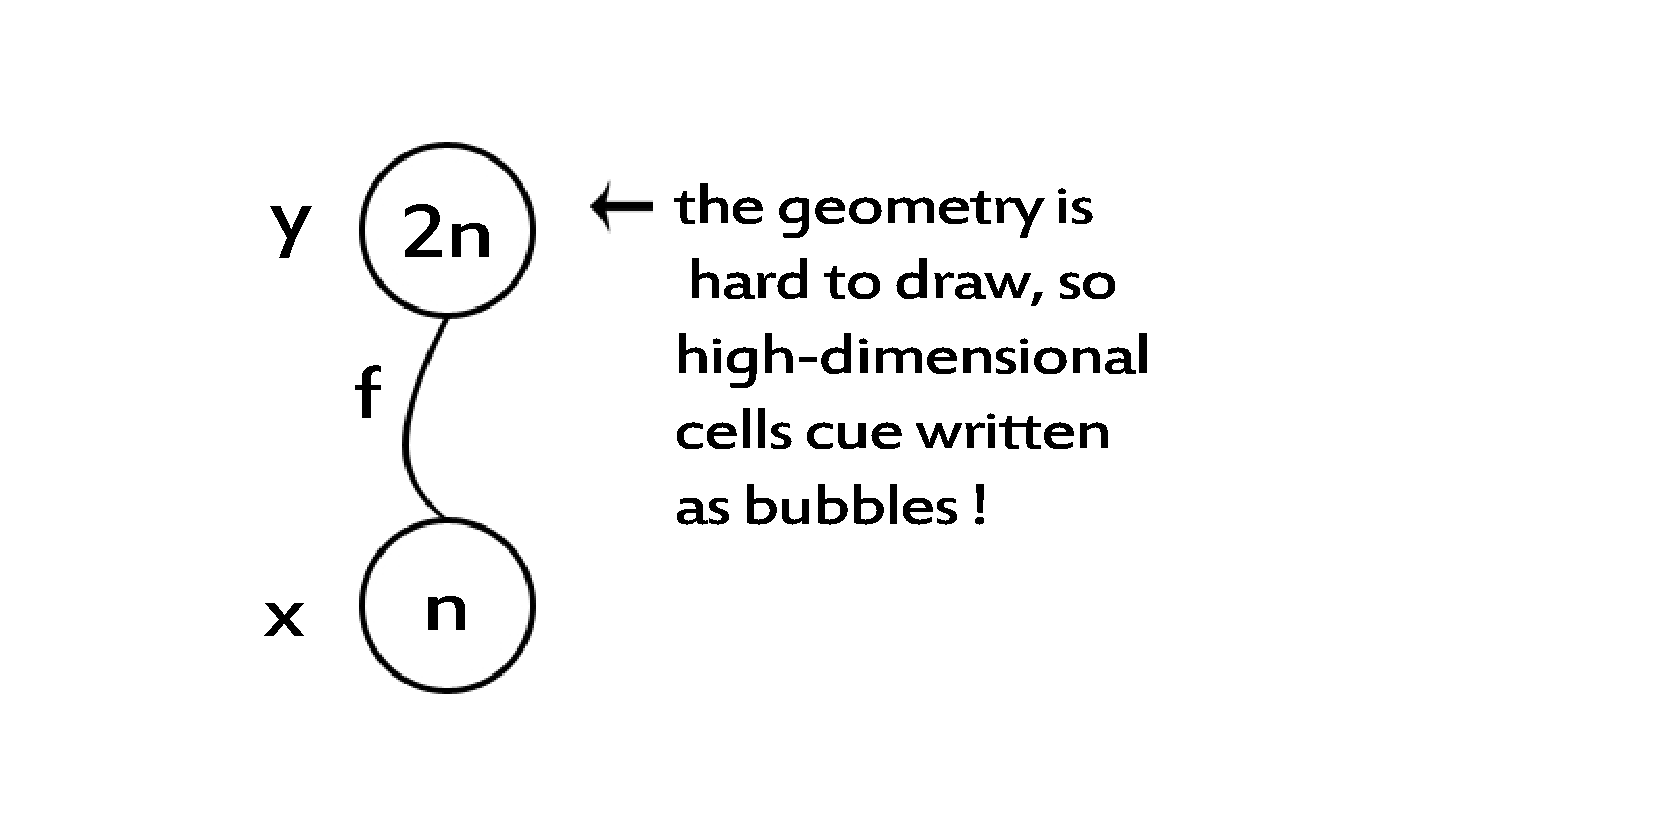
\includegraphics[width=0.3\textwidth]{figures/11.pdf}
\caption{\small Cell diagram of $C(f)$.}
\end{wrapfigure}
Now that we've learned some facts about the squares, we're in a position to apply them to some of the problems that came up earlier.  First, recall that the Hopf invariant $H: \pi_{2n-1} S^n \to \Z$ is defined as follows. $H(f)$ is to be the unique integer (up to sign) for which $x^2=H(f)y$, where $x$ and $y$ are the generators of $H^n(C(f))$ and $H^{2n}(C(f))$ repectively.\footnote{Note that $C(f)$, the cofiber of $S^{2n-1} \stackrel{f}{\to} S^n$ has three cells, one in dimension $0$, $n$ and $2n$.} In particular, $x^2 = H(f) \cdot y \equiv \Sq^n x$ (mod two), so that $H(f)$ is odd iff $\Sq^nx\neq0$.  However, if $n \ne 2^i$, then $\Sq^n$ is decomposable in terms of lower squares, and $\Sq^n x = 0$ since there's no cohomology between $x$ and $y$.  Therefore, we get
\begin{thm}[Adem\footnote{He realized as soon as he got the relations that this was a consequence.}]
If there is an element of odd Hopf invariant on $S^n$, then $n$ is a power of two.
\end{thm}
%\begin{wrapfigure}{r}{0.3\textwidth}
%\centering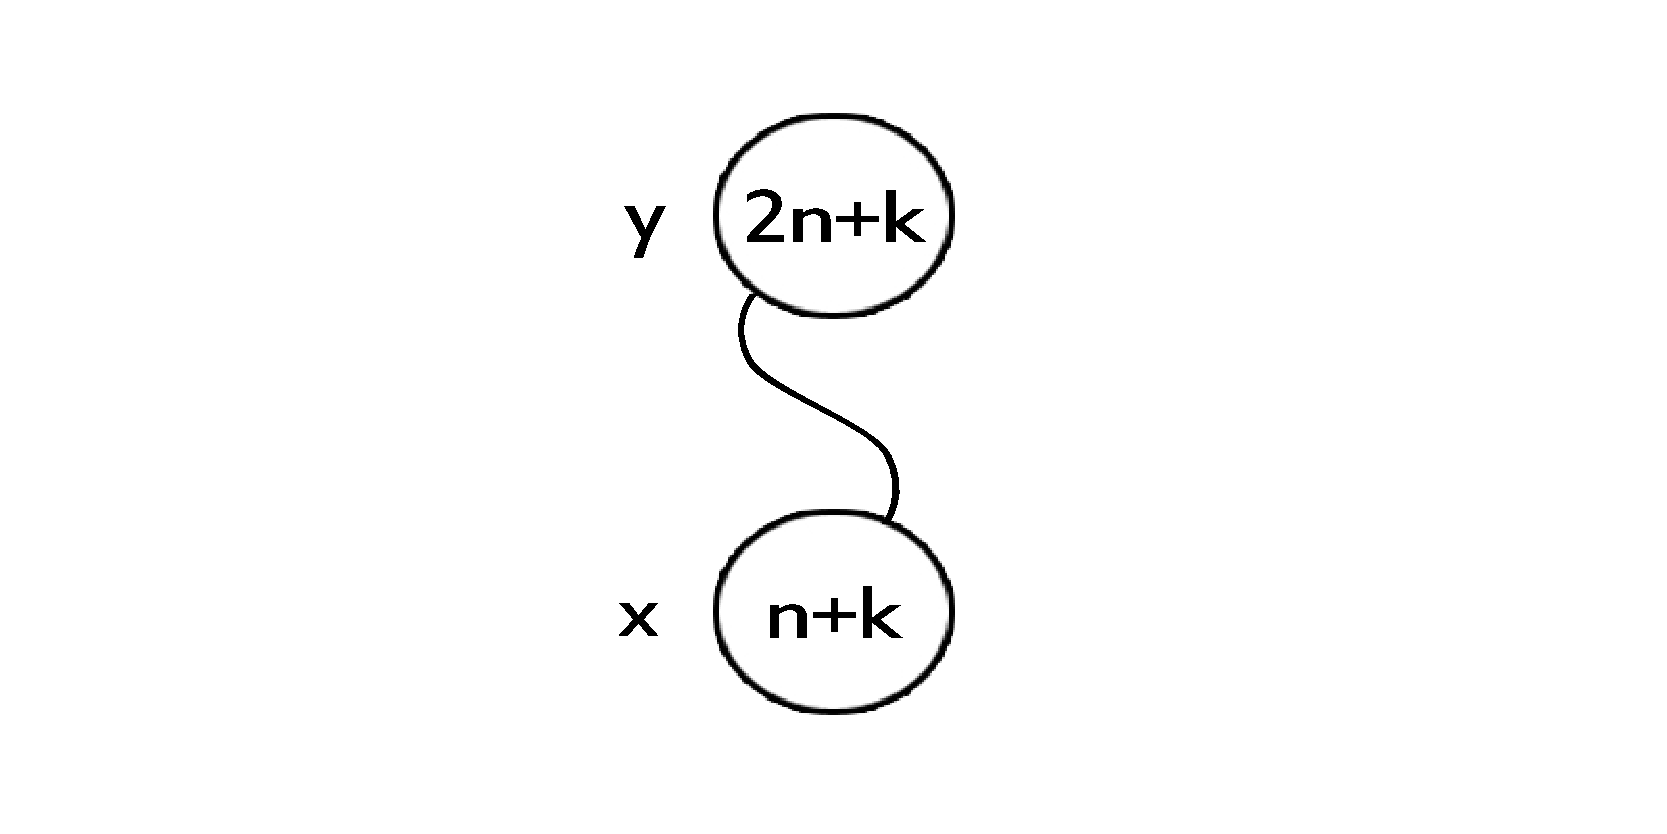
\includegraphics[width=0.3\textwidth]{figures/12.pdf}
%\caption{\small Diagram of $C(g)$.} % this figure should be some kind of staircase of suspensions to see what's going on
%\end{wrapfigure}
Now if $g$ is any map $S^{2n+k-1} \stackrel{g}{\to} S^{n+k} \to C(g)$, then we no longer have a nontrivial cup-product, but we still have $\Sq^n$, so we can define a generalized Hopf invariant $\Htwee(g)$ by $\Sq^n x = \Htwee(g) y$, giving $\Htwee: \pi_{2n+k-1}S^{n+k} \to \Z_2$.  The fact that $\Sq^n$ commutes with suspensions means
\begin{cjointikzcd}
\diagram
   f\dar[mapsto] \\
   \Sigma^kf
%
\diagram
    \pi_{2n-1}S^n\rar["H"]\dar & \Z\dar\\
    \pi_{2n+k-1}S^{n+k}\rar["\Htwee"] &\Z/2
\end{cjointikzcd}
commutes.  $\pi_{2n+k-1} S^{n+k}$ is independent of $k$ for $k \ge 1$; in other words we have turned the unstable question into a related stable one.

Recall next another fact we had, more directly related to the vector field problem: if $S^{n-1}$ has $(k-1)$ everywhere linearly independent vector fields, then $nL \onto \RP^{k-1}$ is fiber homotopy trivial, and this in turn implies the existence of a ``coreduction''
\begin{ctikzcd}
T(nL\downarrow\RP^{k-1}) \hskip-2ex\rar[phantom,"\cong"] &\hskip-2ex \Sigma^n \RP^{k-1}_+ \rar & S^n \\
S^n \uar \ar[urr,"\simeq"',end anchor={south west}]
\end{ctikzcd}
Now we're in a position to study, using the squares, the question of when we can split off the $S^n$ from $T(nL)$.  Remember that we found
\[
T(nL\downarrow\RP^{k-1}) = \RP^{n+k-1}/\RP^{n-1} =: \RP^{n+k-1}_n
,\]
called ``stunted projective space''.  Its mod 2 cohomology is $\Htwee^*(\RP^{n+k-1}_n) = \langle x^n, x^{n+1}, \ldots, x^{n+k-1} \rangle$, where $|x^i| = i$, and it comes in an obvious way from the cohomology of $\RP^{n+k-1}$.  Now the coreduction above implies that the class $x^n$ in $\Htwee^n \RP^{n+k-1}_n$ pulls back from the generator of $\Htwee^n S^n$.  Thus $\Sq^i$ for $i > 0$ is trivial on $x^n$ since it is on $S^n$. That is, $\Sq x^n=x^n$.  Now $x \in \Htwee^1 \RP^{n+k-1}$ is a 1-dimensional class, so $\Sq x = x + x^2 = x(1+x)$, and as $\Sq$ is a homomorphism, $\Sq x^n = x^n(1+x)^n$. %and we have shown that the fiber homotopy triviality of $nL \onto \RP^{k-1}$ implies that we've calculated this same square another way:
\[
\Sq x^n = x^n(1 + x)^n = x^n
,\]
which implies that $(1+x)^n \equiv 1 \pmod{x^k}$.  Write $n = \sum_{i \in I} 2^i$, a sum of distinct powers $i \in I$ of 2.  Then $\nu(n)$ is the smallest $i$ occuring in $I$ (where $n=\textup{odd}\cdot2^{\nu(n)}$ as above), and
\[
(1+x)^n = \prod_{i \in I} (1 + x)^{2^i} = \prod_{i \in I} (1 + x^{2^i}) = 1 + x^{2^\nu} + \hbox{higher powers}
.\]
That $(1 + x)^n \equiv 1 \pmod{x^k}$ implies that $2^\nu \ge k$.  Recall that our goal is to show that $\rho(n) - 1$, the number of linearly independent vector fields on $S^{n-1}$ which we constructed using Clifford algebras, is equal to the actual number of linearly independent vector fields on $S^{n-1}$ by bounding it above.  Here's a table of $\nu(n)$, $2^{\nu(n)}$, and $\rho(n)$ for some small $\nu(n)$:
\[
\begin{array}{c|cccccc}
\nu(n) & 0 & 1 & 2 & 3 & 4 & 5 \\
\hline
2^{\nu(n)} & 1 & 2 & 4 & 8 & 16 & 32 \\
\hline
\rho(n) & 1 & 2 & 4 & 8 & 9 & 10.
\end{array}
\]
For $\nu(n) \le 3$, then, we have obtained an exact answer, but asymptotically, we're doing pretty badly.

There's another approach to this sort of calculation with Thom spaces and squares.  Suppose that $E$ is an $S^{n-1}$-bundle over a base $B$, which we will always assume to be connected. There is an inclusion into the fiberwise mapping cone $C_B E$, a disk bundle:
\begin{ctikzcd}
S^{n-1}\rar&E\rar[hook]\dar&C_BE\dar&D^n\lar\\
&B\rar[equal]&B
\end{ctikzcd}
and $T(E) = C_B E / E$.  So $\Htwee^* (T(E)) = H^*(C_B E, E)$.  Now we can use the relative Serre spectral sequence to get a spectral sequence
\[
E_2^{s,t}=H^s(B, \{H^t(D^n, S^{n-1})\}) \Rightarrow \Htwee^{s+t}( T(E))
.\]
But this spectral sequence has $E_2^{s,t}\neq0$ only when $t=n$, so that that everything collapses by the $E_2$ page, and we obtain isomorphisms $H^*(B, \{H^n(D^n, S^{n-1})\}) \cong \Htwee^{*+n} (T(E))$.  In general $B$ is not simply connected, so we need twisted coefficients.  If the system of local coefficients is trivial, then this isomorphism is the Thom isomorphism.  An orientation of $E$ is then just that: a choice of trivialization of this local coefficient system.

Working over $\Z_2$ coefficients, this coefficient system is already canonically trivial, so the concern about orientation doesn't mean anything, and we get $H^*(B; \Z_2) \cong \Htwee^{*+n} (T(E))$ anyway.  For example, in the case of $nL \onto \RP^{k-1}$ we see trivially that the isomorphism comes from multiplication by $x^n$.  This comes out in general from the multiplicative structure of the spectral sequence, as follows.

First, $1\in H^0 (B)$ corresponds under the Thom isomorphism to some $u \in \Htwee^n (T(E))$, called the ``Thom class''.  Now $\Htwee^* (T(E)) = H^*(C_B E, E)$ is a module over $H^* (B)$ via the ``cup product'' pairing, the composite:
\begin{ctikzcd}
H^*(B) \otimes H^*(C_B E, E)\rar["p^*\otimes1"]&H^*(C_B E) \otimes H^*(C_B E, E)\rar["\smile"]& H^*(C_B E, E)
\end{ctikzcd}
We justify calling this a cup product because $C_BE$ is a disk bundle and $p^*$ is an isomorphism, so we can suppress the pullback part of the operation. The Thom isomorphism says that cup-product by the Thom class $u$ is an isomorphism $\smile u: H^* (B) \cong \Htwee^* (T(E))$.

This enables us to talk about $\Htwee^* (T(E))$ without much reference to $T(E)$ beyond the Thom class.  For example, suppose we wished to calculate $\Sq y$ for some $y\in \Htwee^*( T(E))$. Now $y=xu = x \smile u$, for some unique $x \in H^* B$, and $\Sq y = (\Sq x)(\Sq u)$ by the Cartan formula, so all we need to know is $\Sq u$.  Again using the Thom isomorphism, we write $\Sq^k u = w_k u$, where $w_k \in H^k B$. We call $w_k = w_k(E)$ the ``$k$th Stiefel-Whitney class of $E$'', and we write $w = \sum_{k \ge 0} w_k$, the ``total Stiefel-Whitney class of $E$''.

Of course, if $V$ is a vector bundle, we write $w(V)$ for $w(S(V))$. The following facts follow immediately:
\begin{itemize}
\item $w_k$ depends only on the fiber homotopy type of the sphere bundle.
\item $\Sq^0 u = u$, so $w_0 = 1$.
\item $w_k = 0$ for $k > n$.
\item External Whitney sum formula:\footnote{Whitney says this is the hardest theorem he ever proved, but he had the wrong definition of Stiefel-Whitney classes.} $w(E'\mathop{\widehat\ast}E''\downarrow B'\times B'')=w(E'\downarrow B')\times w(E''\downarrow B'')$ for sphere bundles $E'\downarrow B'$ and $E''\downarrow B''$.
\item Internal Whitney sum formula: $w(E'\mathop{\ast_B} E''\downarrow B)=w((E'\downarrow B)\smile w(E''\downarrow B))$ for sphere bundles $E'\downarrow B$ and $E''\downarrow B$.
In particular, $w(V'\oplus V'')=w(V')\smile w(V'')$ for vector bundles $V',V''$ over $B$.
\item Stability: One calculates $w(n\varepsilon) = 1$, so that $w(V \oplus n\epsilon) = w(V)$  (using the Whitney sum formula).
\end{itemize}
\begin{lem}\label{ThomClassLem}
Suppose that $E\downarrow B$ is an $S^{n-1}$-bundle over a connected base, and that $s:S^n\to T(E)$ is the inclusion of copy of $S^n$ over the basepoint, and that $u\in H^n(T(E))$ is the Thom class. Then $s^*(u)$ is the generator $\mathit{o}\in H^n(S^n)$ that corresponds to the standard orientation\footnote{That is, the orientation on $S^n=(D^n,S^{n-1})$ which was used to trivialise the coefficient system used in the Serre spectral sequence which provided the Thom isomorphism.} of $S^n$.
%Alternatively, $u$ is the class dual to $s_*(S^n)\in H_n(T(E))$.
\end{lem}
\begin{proof}
This follows by naturality of the Thom isomorphism for oriented maps of oriented $S^{n-1}$-bundles, once it has been checked for the trivial $S^{n-1}$-bundle $\mathcal{E}=S^{n-1}\downarrow*$ (a simple task). Consider the map of oriented $S^{n-1}$-bundles (shown at left):
\begin{cjointikzcd}
\diagram[2]
    \mathcal{E}\ar[r]\ar[d]&E\ar[d]\\
    \ast\ar[r]&B
\diagram
    \mathllap{S^n={}}T(\mathcal{E})\ar[r]&T(E)\\
    S^n\uar[equal]\ar[ur]
%
\diagram
    u_\mathcal{E}\dar[equal] &\lar[mapsto]u_E\dlar[mapsto]\\
    \mathit{o}
\end{cjointikzcd}
This map induces the commuting diagram in the middle: a map of Thom spaces relative to $S^n$. Using this commuting diagram, we can calculate $s^*(u_E)$ in two different ways (at right) to obtain the result.
\end{proof}
\begin{proof}[Proof of Whitney sum formula]
 Let $E' \downarrow B'$ be an $S^{n-1}$-bundle and $E'' \downarrow B''$ be a $S^{m-1}$-bundle; let $E\downarrow B$ be the fiberwise join, an $S^{m+n-1}$-bundle.  Now, $T(E) = T(E') \sprod T(E'')$, and moreover, $u = u' \sprod u''$. To see this, recall that the inclusion $S^{n+m}\hookrightarrow T(E)$ is the wedge of the inclusions $S^{n}\hookrightarrow T(E')$ and $S^{m}\hookrightarrow T(E'')$. Now by the characterisation of $u$ in lemma \ref{ThomClassLem}, we see that $u$ pulls back to the orientation generator in $H^{n+m}(S^n\sprod S^m)$, which is the wedge of the orientation generators in $H^n(S^n)$ and $H^m(S^m)$.

Thus, $\Sq u = \Sq(u' \sprod u'') = \Sq u' \sprod \Sq u''$. Note that the first expression models $w(E) \smile u$, while the third expression models $w(E') \sprod w(E'') \smile u' \sprod u''$.  Therefore, $w(E) = w(E') \sprod w(E'')$.
\end{proof}

Now the Thom class of $nL \onto \RP^{k-1}$, as we saw, is $x^n$.  So $w(L) = 1 + x$, and $w(nL) = (1+x)^n$.  So $nL \onto \RP^{k-1}$ is fiber homotopy trivial only if $(1+x)^n \equiv 1 \pmod{x^k}$, which is the same result we obtained before.  Now the program is to improve the results by pursuing a similar set of results in $KO$-theory.

% >>>
\fi
\begin{SummaryNote}
\Bullet Using the decomposability of $\Sq^i$ for $i\neq2^j$, there can only be an element of Hopf invariant one in $\pi_{2n-1}(S^n)$ if $n=2^j$.

\Bullet $\Sq x^n=x^n(1+x)^n$, where $x^n\in\Htwee^n(\RP^{n+k-1}_n)$. If there is a coreduction, then $\Sq x^n$ must equal $x^n$. Thus, a necessary condition for $k-1$ fields on $S^{n-1}$ is that $(1+x)^n\equiv 1$ in $\Z_2[x]/(x^k)$, which implies $2^{\nu(n)}\geq k$.

\Bullet For an oriented $S^{n-1}$-bundle $E$, $\Htwee^*(T(E))$ is an $H^*(B)$-module under ``$\smile$'':
\begin{ctikzcd}
H^*(B) \otimes H^*(C_B E, E)\rar["p^*\otimes1"]&H^*(C_B E) \otimes H^*(C_B E, E)\rar["\smile"]& H^*(C_B E, E)
\end{ctikzcd}

\Bullet Defined the Thom class $u\in H^n(T(E))$ such that $\smile u$ is the Thom isomorphism $H^*(B)\to\Htwee^{*+n}(T(E))$.

\Bullet The Stiefel-Whitney classes $w_i(E)\in H^i(B)$ are defined by $w(E)\smile u=\Sq u$. They vanish for $i>n$, and $w_0=1$. They satisfy the Whitney sum formula $w(V\oplus W)=w(V)\smile w(W)$, and are stable: $w(V\oplus \epsilon)=w(V)$.
\end{SummaryNote}



\section{Structure on \texorpdfstring{$K$}{K}-theory} % <<<
\label{StructureOnKtheory}
\ifx\OutputStructureOnKtheory\undefined\else
This isn't a course about $K$-theory, it's a course that uses $K$-theory.  So we're not going to see proofs of lots of basic theorems of $K$-theory; in particular I'm not going to prove the periodicity theorem.  However, we will need some facts which we'll review now.

Recall that we previously defined the group $\KOtwee(X)$, and by doing the same constructions using complex vector bundles we get $\Ktwee(X)$.  Let's see what $\Ktwee S^2$ is.  $S^2$ splits into contractible hemispheres $D_\pm$ over which any vector bundle is trivial, $D_\pm \times \C^n$.  The construction of a vector bundle on $S^2$ therefore amounts to choosing over each point on the equator $S^1$ a linear isomorphism $\C^n \to \C^n$ in a continuous manner, i.e., a map $S^1 \to GL_n(\C)$.  So, $\Vect_{n,\C}(S^2) \cong \pi_1 GL_n(\C)$.  This way of constructing vector bundles is called the ``clutching construction.''  There are compatible deformation retractions
%
\begin{ctikzcd}
\cdots\rar[hook] & GL_n(\C)\rar[hook]\dar &GL_{n+1}(\C)\rar[hook]\dar&\cdots\\
\cdots\rar[hook] & U(n)\rar[hook]&U(n+1)\rar[hook]&\cdots\\
\end{ctikzcd}
%
and hence we may assume all our maps have codomain $U(n)$ instead.\footnote{The existence of such a retract implies that there is a functorial way to assign Hermitian inner products to complex vector bundles.}  Each inclusion on the bottom row occurs as the fiber of a bundle\footnote{Note that $U(n+1)$ acts on $S^{2n+1}$. Choosing a basepoint $b\in S^{2n+1}$, the map $U(n+1)\to S^{2n+1}$ given by $x\mapsto xb$ is a fibration with fiber the stabiliser of $b$. Of course, the stabiliser is $U(n)$.} $U(n+1) \to S^{2n+1}$, and hence we calculate using the long exact sequence of homotopy groups that $\pi_1 U(n) \cong \pi_1 U(n+1)$ induced by these inclusions for $n \ge 1$. In particular, $\pi_1 U(1) \cong \pi_1 S^1 = \Z$, so that $\pi_1 U(n)\simeq \Z$, where homotopy class corresponding to $k\in \Z$ is that of the map $z\mapsto\textup{diag}(z^k,1,1,\ldots)$ for $z\in S^1=U(1)$.

Now if $V_{n,k}$ is the $n$-dimensional complex bundle obtained by clutching along the element of $\pi_1 U(n)$ corresponding to $k\in\Z$, it is not hard to see that $V_{n,k}\oplus V_{n',k'}$ is isomorphic to $V_{n+n',k+k'}$. From this we see that $\Ktwee(S^2) \cong \Z$, generated by $[V_{1,1}]-1$.

Now we have represented the generator of $\pi_1 U(1)$ as the identity, which as a clutching function represents $\bundle{L} \onto \CP^1 \simeq S^2$, the tautological (complex) line bundle.  Hence, a generator of $\Ktwee S^2$ is $[\bundle L] - 1$.  Similarly, since all the unitary groups are connected, $\Ktwee(S^1) = 0$.

\begin{fact}
In the real case, we have $\KOtwee(S^8) = \Z$, generated by the tautological Cayley $\mathbb{H}$-line bundle, considered as a 4-dimensional real bundle over $\mathbb{H}P^2 \simeq S^8$. (What happens if we use octonions?) % is this last bit right?  and what about the octonions?
\end{fact}

\begin{thm}[Bott periodicity]
\begin{align*}
\Ktwee (X) \otimes \Ktwee (S^2) & \stackrel{\cong}{\to} \Ktwee(X \sprod S^2) \\
\KOtwee (X) \otimes \KOtwee (S^8) & \stackrel{\cong}{\to} \KOtwee(X \sprod S^8).
\end{align*}
\end{thm}

A word on this tensor product: an element of $\Ktwee (X)$ is a ``virtual vector bundle'' $V - m$, where $m$ is the trivial bundle of dimension $m = \dim V$.  If $V - m \in \Ktwee(X)$ and $W - n \in \Ktwee(S^2)$, then we define earlier their exterior tensor product over $X \times S^2$ in the obvious way: $(V - m)\hat\otimes(W - n) = V \hat\otimes W - m \hat\otimes W - V \hat\otimes n + m \hat\otimes n$.  Consider now what this bundle looks like over $X \vee S^2 \subseteq X \times S^2$: on $X \times \ptspace$, $W$ is trivial, so we get $V \hat\otimes n - m \hat\otimes n - V \hat\otimes n + m \hat\otimes n = 0$; on $\ptspace \times S^2$ we see that $V$ is trivial, so we get $m \hat\otimes W - m \hat\otimes W - m \hat\otimes n + m \hat\otimes n = 0$.  Hence, the bundle $(V - m) \hat\otimes (W - n)$ is trivial over $X \wsum S^2$, and so pulls back from a vector bundle over $X \sprod S^2$.  This at least exhibits the map above.

Next let's see how the periodicity theorem can be used to make $KO$ and $K$ the $0^\textup{th}$ groups of periodic generalized cohomology theories with periods $8$ and $2$ respectively.  The first thing we observe is that $\KOtwee$ is representable; recall that $\KOtwee(X)$ is given by pointed homotopy classes of maps $X \to BO \times \Z$, denoted $[X, BO \times \Z]$ (we'll start writing $B$ for $BO \times \Z$).  Cued by the suspension isomorphism from singular cohomology, for $n \ge 0$ we define:
\begin{align*}
\qquad\qquad\qquad
\KOtwee^{-n} (X) & = \KOtwee(\Suspend^n X)\hbox{\ for $n\geq0$}, \\
\KOtwee^n(X) & = \KOtwee(\Suspend^{8k-n}X) \hbox{\ for any $k$ with $8k > n$}, \\
KO^*(X) &= \KOtwee^* X_+, \\
KO^*(X, A) & = \KOtwee^*(X \cup CA) \textup{\ when $A\hookrightarrow X$ is a cofibration.}
\end{align*}

For this to be considered a cohomology theory we need some long exact sequences.  Now its a general fact that for a map of pointed spaces $f: A \to X$ if we take the mapping cone $A \stackrel{f}{\to} X \to X \cup_f CA = C(f)$, then the sequence
\[
[A, B] \from [X, B] \from [X \cup CA, B]
\]
is exact.  Moreover, when $B$ is an $H$-space then the induced homomorphisms of groups are exact.  Now we can continue; that is, take the mapping cone of $X \to X \cup_f CA$:
\[
A \stackrel{f}{\to} X \stackrel{i}{\to} X \cup_f CA \to (X \cup_f CA) \cup_i CX \to \cdots
\]

%\begin{wrapfigure}{r}{0.4\textwidth}
%\centering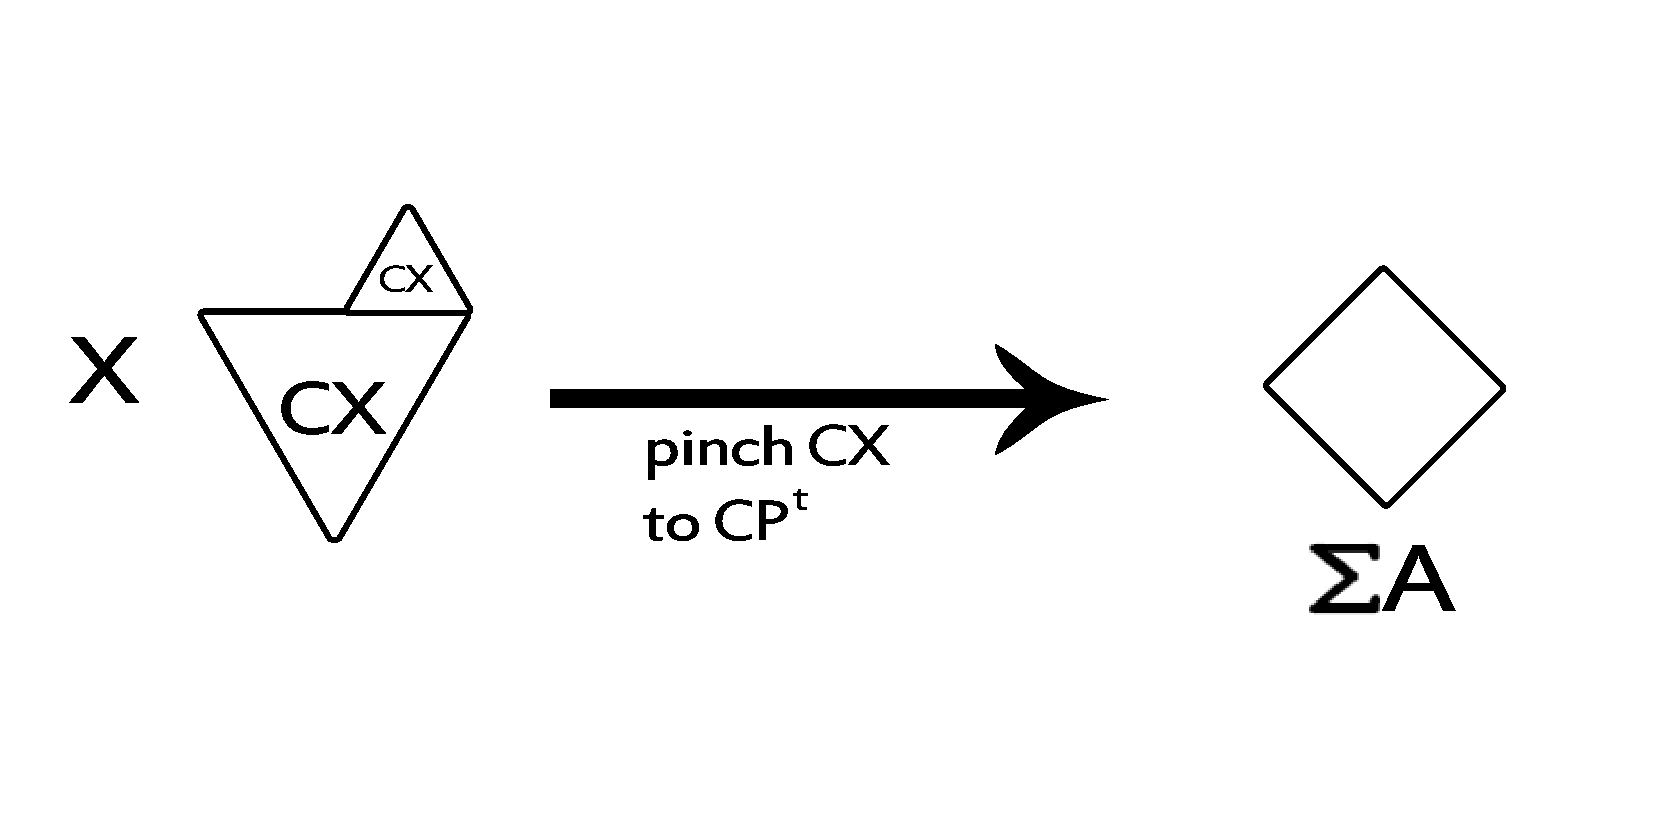
\includegraphics[width=0.3\textwidth]{figures/13.pdf}
%\caption{\small The going-around quotient.}
%\end{wrapfigure}
Now, if $f$ is nice enough, $X \cup CA$ will be homotopic to $X / A$.  Certainly $(X \cup CA) \cup CX \simeq (X \cup CA)/X$, so the sequence becomes
\[
A \to X \to X \cup CA \to \Suspend A \to \Suspend X \to \cdots
,\]
and moreover the map $\Suspend A \to \Suspend X$ can in fact by given by $\Sigma f$ up to homotopy.  This sequence is called the ``Barratt-Puppe'' sequence.  We can then apply the Hom-functor $[-, B]$ to get a long exact sequence\footnote{Applying $[-, Z]$ will give a long exact sequence of pointed sets for any $X$.  Since our $Z = B$ is an $H$-group, this gives a long exact sequence of groups.}
\[
[A, B] \from [X, B] \from [X \cup CA, B] \stackrel{\delta}{\from} [\Suspend A, B] \from [\Suspend X, B] \from \cdots
.\]
Identifying groups as above, we produce a long exact sequence
\[
\KOtwee^0 (A) \from \KOtwee^0(X) \from KO^0(X, A) \from \KOtwee^{-1}(A) \from \KOtwee^{-1}(X) \from \cdots
,\]
and via periodicity we have the full long exact sequence
\[
\cdots \from KO^1(X, A) \from \KOtwee^0 (A) \from \KOtwee^0(X) \from KO^0(X, A) \from \KOtwee^{-1}(A) \from \KOtwee^{-1}(X) \from \cdots
.\]
This justifies our choice of definition of $\KOtwee^*$ above.  This whole setup works similarly for complex $K$-theory.

Now it's an important fact about $\Ktwee^* (X)$ that it's a commutative ring: we calculated $\Ktwee^0 (S^1) = 0$ and $\Ktwee^0 (S^2) = \Z$ with generator $(\bundle{L} - 1)$, which gives a generator $p \in \Ktwee^{-2} (S^0) = K^{-2} (\ptspace)$, called the ``periodicity element.''  So $K^* \eqdef K^* (\ptspace) = \Z[p^{\pm 1}]$, the Laurent series ring, where $|p| = -2$.  Similarly, there is a ring structure for $KO^*$:
\[
\begin{array}{c|ccccccccc}
n & 0 & 1 & 2 & 3 & 4 & 5 & 6 & 7 & 8 \\
\hline
KO^{-n} (\ptspace) & \Z & \Z_2 & \Z_2 & 0 & \Z & 0 & 0 & 0 & \Z \\
\mathrm{generator} & 1 & \eta & \eta^2 & & q & & & & p,
\end{array}
\]
with relations $2\eta = 0$, $\eta^3 = 0$, $\eta q = 0$, $q^2 = 4p$, where $p$ is the periodicity element. For example, $KO^{-10}(\ptspace) = \langle p\eta^2 \rangle \cong \Z_2$ and $KO^{6}(\ptspace) = \langle p^{-1}\eta^2 \rangle \cong \Z_2$, so that $KO^*$ is the ring with generators $\eta,q,p^{\pm1}$ and the given relations.

Unfortunately, we shall need more than just the ring structure; we'll need operations.  One way to get operations in $K$-theory is to look for operations on vector spaces, apply these fiber-wise to get operations on vector bundles, and then squeeze out operations on $K$-theory.  The most useful of these is $V \mapsto \Lambda^k(V)$, the $k$th exterior power.  By means of this method we get a $k^\textup{th}$ exterior power bundle $\Lambda^k E \downarrow B$ from a bundle $E\downarrow B$.  Unfortunately extending to $K$-theory is hard because $\Lambda^k$ is not additive.

There is, however, a natural isomorphism $\Lambda^k(V \oplus W) = \bigoplus_{i+j = k} \Lambda^i V \otimes \Lambda^j W$.  This (which looks like a Cartan formula) inspires the definition $\Lambda_t(V) = \sum_{i \ge 0} t^i \Lambda^i(V)$.  Now $\Lambda_t(V \oplus W) = \Lambda_t(V) \cdot \Lambda_t(W)$, so the operation still isn't additive, but it's exponential --- it takes sums to products.  That's good enough, as it turns out.  So $\Lambda_t$ induces a homomorphism of commutative monoids $\Lambda_t: \Vect(X) \to 1 + t\,KO(X)\llbracket t \rrbracket$, where the target is the group (under multiplication) of formal power series in $t$ with coefficients in $KO(X)$ and constant term one.

By definition of $KO(X)$, there is a group homomorphism $\lambda_t: KO(X) \to 1+t\,KO(X) \llbracket t \rrbracket$ such that the map $\Lambda_t$ factors:
\begin{ctikzcd}
\Vect(X)\rar["\Lambda_t"]\dar & 1+t\,KO(X)\llbracket t \rrbracket\\
KO(X)\urar["\lambda_t"']
\end{ctikzcd}
That $\lambda_t$ is a group homomorphism is to say that
%\[
$\lambda_t(A + B) = \lambda_t(A) \cdot \lambda_t(B)$
%,\]
for $A, B \in KO(X)$. This behaviour is like that of total Steenrod operations.  Of course if $E$ is a vector bundle, then $\lambda^j(E) = \Lambda^j(E) = 0$ for $j > \dim E$ (where $\lambda^j$ is defined, of course, by $\lambda_t(E) = 1 + \sum_{k \ge 1} t^k \lambda^k(E)$.)

The $\lambda$ operations are all very well, but they are hard to work with because they depend on the ring structure of $KO(X)$.  We really want an additive ``power operation,'' so one thing to try is to take a logarithm, in search of a family of operations $\psi^k$ such that on line bundles we get $\psi^k(L) = L^{\otimes k}$.  Once again, we start with a generating function $\psi_t(x) = \sum_{k \ge 1} \psi^k(x) t^k$, then our conditions on $\psi^k$ become:
\begin{align*}
\psi_t(x + y) & = \psi_t (x) + \psi_t (y), \\
\psi_t(L) & = \sum_{k \ge 1} L^k t^k = \frac{Lt}{1 - Lt}.
\end{align*}
The first obvious candidate is \[\log \lambda_t(x) = \sum_{i=0}^\infty (-1)^i \frac{(\lambda_t(x) - 1)^i}{i} = (\lambda_t(x) - 1) - \frac{(\lambda_t(x) - 1)^2}{2} + \frac{(\lambda_t(x) - 1)^3}{3} - \cdots,\] but unfortunately this has denominators,\footnote{Check the $t^2$ coefficient!} and we don't know what $1/n$ means in $KO(X)$.  Our next guess is $\frac{d}{dt} \log \lambda_t(x) = \frac{\frac{d}{dt} \lambda_t(x)}{\lambda_t(x)}$ (and $\lambda_t(x)^{-1}$ exists), and so we have additivity, the first property.  Now for $L$ a line bundle,
\[
\frac{d}{dt} \log (1 + tL) = \frac{L}{1 + tL}
.\]
Replace $t$ with $-t$ to get $\frac{d}{dt} \log(1 - tL) = \frac{-L}{1 - tL}$.  And, to normalize, multiply by $-t$ to get $\frac{tL}{1 - tL} = \sum_{k \ge 1}^\infty t^k L^k$.  We define the $k^\textup{th}$ ``Adams operation'' applied to $E$, $\psi^k(E)$, to be the coefficient of $t^k$ in \[\frac{-t \frac{d}{dt} \lambda_{-t}(E)}{\lambda_{-t}(E)}.\]
Of course, this construction could be carried out on $K(X)$ as opposed to $KO(X)$.

We seek to prove the following properties of the Adams operations, and will do so by constructing them from another perspective in lecture \ref{BuildingKtheoryOperatorsFromRepTheory}:
%\begin{thm}\textbf{False claim:}
%There exist unique operations $\psi^k: KO(X) \to KO(X)$ such that:
\begin{itemize}
\item $\psi^k$ is a ring homomorphism for each $k$,
\item $\psi^k \psi^l = \psi^{kl}$, and
\item $\psi^k(L) = L^{\otimes k}$ for line bundles $L$ (which we already know).
\end{itemize}
%\end{thm}
\noindent\textbf{Do the properties above characterise the Adams operations on $K(X)$?}

% >>>
\fi
\BoxedNote{
\Bullet $\Ktwee(S^2)=\Z\langle[\bundle L]-1\rangle$ where $\bundle L\downarrow \CP^1$ is the tautologous $\C$-line bundle.

\Bullet $\KOtwee(S^8)=\Z\langle[\bundle L]-4\rangle$, with $\bundle L\downarrow \mathbb{H}P^2$ the tautologous $\mathbb{H}$-line bundle.

\Bullet $\Ktwee(X)$ is extended to a cohomology theory via $K^{-n}X \eqdef K(\Sigma^nX)$ ($n\geq0$) and via periodicity for $n<0$. $\Ktwee^*(\ptspace)=\Z[p^{\pm1}]$ for $p=\bundle L-1\in \Ktwee^{-2}(\ptspace)$ the periodicity element. The same story holds for $\KOtwee$, but it's more complicated.

\Bullet As $\Lambda^t(V\oplus W)\cong\oplus \Lambda^{t_1}(V)\otimes\Lambda^{t_2}(W)$, defining $\Lambda_t(V) \eqdef \sum t^i\Lambda^t(V)$ we get $\lambda_t:KO(X)\to1+t\,KO(X)\llbracket t \rrbracket$ taking sum to product.

\Bullet Using the generating function $-t\frac{d}{dt}\log \lambda_{-t}(E)=\sum t^k\psi^k(E)$, we obtain additive operations on $KO(X)$ such that $\psi^k(L)=L^{\otimes k}$, the ``Adams operations''.

\Bullet \textbf{False claim:} The Adams operations are characterised by three properties:\\\phantom{space}(i) they are ring homomorphisms; (ii) $\psi^k\psi^l=\psi^{kl}$; and (iii) $\psi^k(L)=L^{\otimes k}$.
}
\section{\texorpdfstring{$K$}{K}-theory operations via representation theory} % <<<
\label{BuildingKtheoryOperatorsFromRepTheory}
\ifx\OutputBuildingKtheoryOperatorsFromRepTheory\undefined\else
Previously, we discussed the ring $KO^* = KO^* \ptspace$ and said it was
\[
KO^* = \Z[\eta, q, p^{\pm 1}], |\eta| = -1, |q| = -4, |p| = -8
,\]
along with the relations $2 \eta = 0$, $\eta q = 0$, $\eta^3 = 0$, and $q^2 = 4p$.  Furthermore we defined operations $\psi^k$ on $KO(X)$ which \textbf{(will be shown to have the following properties)} are ring homomorphisms and satisfy $\psi^k \psi^l = \psi^{kl}$ and, for line bundles $L$, $\psi^k L = L^{\otimes k}$.  In order to get a better handle on these, we need some character theory, which belongs to the broader field of representation theory.

Let $G$ be a compact Lie group (e.g., $G=U(n)$, the group of $n\times n$ unitary matrices).  A representation of $G$ is a finite-dimensional complex vector space $V$ together with a linear action of $G$.  Two representations $V$ and $V'$ are isomorphic if and only if there is a $G$-equivariant linear isomorphism $\alpha: V \stackrel{\cong}{\to} V'$.

Choose any Hermitian inner product on $V$.  By averaging over the group,\footnote{As $G$ is a compact Lie group it admits a Haar measure, so we can `average'.} we can form a $G$-invariant inner product $\langle - , - \rangle$. Then $G$ acts by unitary transformations on $V$, that is $\langle gx, gy \rangle = \langle x, y \rangle$, for all $g\in G$.  Picking an orthonormal basis gives each $g\in G$ as a unitary matrix, and the representation becomes a map $\rho: G \to U(n)$, where $\rho$ is a continuous homomorphism.  With these data, an isomorphism of representations looks like a matrix $M$ in terms of these bases such that $\rho'(g) = M \rho(g) M^{-1}$ for all $g \in G$.

Once we have matrices it makes sense to talk about the trace; define $\chi_V(g) = \tr(\rho(g))$.  This gives a function $\chi_V: G \to \C$, called the ``character of $V$.''  We call $\chi_V$ a ``class function'' because it is constant on conjugacy classes\footnote{The trace is invariant under cyclic permutations.} in $G$.  In particular if two representations $V$ and $V'$ are isomorphic, then $\chi_V = \chi_{V'}$.
Using characters is by far the easiest way to understand representations, and in fact they tell us everything, as we will see in fact \ref{chiisinjectivo}.

Define $\Rep_n(G) \eqdef \Hom(G, U(n)) /\textup{conjugacy}$.  Then $\Rep(G) \eqdef \coprod_n \Rep_n G$ is a semiring with addition given by $\oplus$ and multiplication by $\otimes$.\footnote{$G$ acts diagonally on the tensor produuct of $G$-modules.} Applying the Grothendieck construction to $\Rep(G)$ we obtain the ``representation ring'' of $G$, denoted $R(G)$.  The map $V \to \chi_V$ induces a map $\chi: R(G) \to \{\hbox{class functions $G \to \C$}\}$.

\begin{fact}
$\chi_{V \oplus W} = \chi_V + \chi_W$, and $\chi_{V \otimes W} = \chi_V \chi_W$.
\end{fact}
The second fact is true because $\tr(A \otimes B) = \tr A \tr B$ for matrices $A$ and $B$.\footnote{If $A \in U(m) \cong \operatorname{Isom} \C^m$ and $B \in U(n) \cong \operatorname{Isom} \C^n$, then $A \otimes B \in U(mn) \cong \operatorname{Isom} (\C^m \otimes_\C \C^n)$. Note that here we implicity choose an identification of $\C^m\otimes_\C\C^n$ with $\C^{mn}$ --- there is a ``standard'' way to do so in which $A\otimes B$ is represented by the Kronecker product of matrices $A$ and $B$.}  Indeed, any unitary matrix has a diagonalization\footnote{``This is the deepest fact of the lecture.''} and if $\{x_1, \ldots, x_m\}$ and $\{y_1, \ldots, y_n\}$ are bases of eigenvectors for $A$ and $B$, then $\{x_i \otimes y_j\}$ is a basis of eigenvectors for $A \otimes B$, and the eigenvalue for $x_i \otimes y_j$ is the product of the eigenvalues for $x_i$ in $A$ and $y_j$ in $B$.

\begin{fact}\label{chiisinjectivo}
$\chi$ is injective, and in fact $R(G) \otimes_\Z \C \stackrel{\cong}{\to} \{\hbox{class functions}\}$.
\end{fact}
Recall that the first construction of the Adams operations used an operation on vector spaces to yield an operation on bundles, and then finally an operation on $K$-theory.  Now we shall use representations to construct new vector bundles out of old ones.  First we will need the notion of the principal bundle associated to a vector bundle: if $E \downarrow X$ is an $n$-dimensional complex vector bundle and $X$ is paracompact, you can pick a Hermitian metric on $E$ and get an orthonormal basis on each fiber (meaning, a continuously varying choice of orthonormal basis).  Let $P(E)$ be the set of all ordered orthonormal bases on fibers.  Another way to think about it is that each point in $P(E)$ is a linear isometry $\C^n \cong E_x$.  Now there is a projection $P(E) \to X$; there is a fiberwise action of $U(n)$ on $P(E)$ given by composition: if $\alpha \in P(E)$ determines $\alpha: \C^n \stackrel{\cong}{\to} E_x$, then for $g \in U(n)$ there is a triangle of isomorphisms:
\begin{ctikzcd}[column sep=tiny]
\C^n\ar[rr,"\alpha"] & & E_x\\
 & \C^n \ular["g"]\urar["\alpha g"']
\end{ctikzcd}
It is clear that this action gives $P(E) \downarrow X$ the structure of a principal $U(n)$-bundle, the ``associated principal bundle to $E$.''

Now the construction of $P(E)$ involved the choice of a Hermitian metric $\langle - , - \rangle$ for $E \downarrow X$.  But if $\langle -, - \rangle'$ is another Hermitian metric for $E \downarrow X$, then so\footnote{A Hermitian inner product is required to satisfy $\langle x, x \rangle > 0$ for $x \ne 0$; this provides the non-degeneracy of $\langle - , - \rangle_t$.} is $t \langle -, - \rangle' + (1-t) \langle -, - \rangle = \langle - , - \rangle_t$ for $0 \le t \le 1$. Thus we obtain a metric for the bundle $E \times I \downarrow X \times I$.
Now the restriction of $P(E \times I) \downarrow X \times I$ to $X \times \{0\}$ is $P_{\langle-,-\rangle}(E)$, while the restriction to $X \times \{1\}$ is $P_{\langle-,-\rangle'}(E)$, so that $P_{\langle-,-\rangle}(E) \cong P_{\langle-,-\rangle'}(E)$ as $U(n)$-bundles.

Now let $V$ be a representation of $U(n)$.  Then from a complex vector bundle $E \downarrow X$, we can form the bundle $\alpha_V(E) = (P(E) \times_{U(n)} V) \downarrow X$, yielding a new vector bundle with fiber $V$.

Now fix an $n$-dimensional vector bundle $E$. Clearly $\alpha_{V \oplus W}(E) = \alpha_V(E) \oplus \alpha_W(E)$, so that $V \mapsto \alpha_V(E)$ defines an additive homomorphism $\Rep(U(n)) \to \Vect(X) \to K(X)$. By the universality property of the Grothendieck construction this extends to $R (U(n))$:
\begin{ctikzcd}
\Rep(U(n))\dar\rar["\alpha_-(E)"] &|[inner ysep=0.2em]| K(X)\\
R(U(n))\urar["\theta\mapsto\theta(E)"{sloped, anchor=north}]
\end{ctikzcd}

Turning this around, a fixed $\theta \in R (U(n))$ assigns to an $n$-dimensional vector bundle $E \downarrow X$ a well-defined element $\theta(E)$ of $K(X)$; what we really want is to assign to an element $E$ of $K(X)$ another element of $K(X)$.  In particular, we have to worry about different values of $n$; moreover, we want to get an additive homomorphism.

It will suffice to choose $\theta_n \in R(U(n))$ for $n \ge 0$ in such a way that $\theta_m (E^m) \oplus \theta_n (F^n) = \theta_{m+n}(E \oplus F)$ in $K(X)$. This data can then be used to define an additive homomorphism $\theta:\coprod_n\! \Vect_n(X) \to K(X)$, which (by universality) extends to an operation $\theta:K(X)\to K(X)$.

Taking the direct sum of representations gives a homomorphism $R(U(m)) \times R(U(n)) \stackrel{\oplus}{\to} R(U(m) \times U(n))$. One way to view this is that the projections $U(m) \stackrel{\pi_1}{\from} U(m) \times U(n) \stackrel{\pi_2}{\to} U(n)$ induce pullbacks
\[R(U(m))\stackrel{\pi_1^*}{\to}R(U(m) \times U(n))\stackrel{\pi_2^*}{\from}R(U(n))\textup{ which induces } R(U(m)) \oplus R(U(n)) \stackrel{\oplus}{\to} R(U(m) \times U(n)).\]
On characters, the map $\oplus$ is defined by $\chi_{\theta_m \oplus \theta_n}(M, N) = \chi_{\theta_m}(M) + \chi_{\theta_n}(N)$.  On the other hand, the inclusion
\[U(m) \times U(n) \stackrel{\sigma}{\to} U(m+n)\text{ given by }(M, N) \mapsto \left[\begin{array}{c|c}M & 0 \\ \hline 0 & N\end{array}\right]
\textup{ induces }\sigma^*: R(U(m+n)) \to R(U(m) \times U(n)).\]
On characters, $\sigma^*$ is defined by $\chi_{\sigma^* \theta_{m+n}}(M, N) = \chi_{\theta_{m+n}}\left(\sigma(M,N)\right)$.

We define $\theta = \{\theta_n \in R(U(n)), n \ge 0\}$ to be an ``additive sequence'' when $\theta_m \oplus \theta_n = \sigma^* \theta_{m+n}$ for all $m, n \ge 0$. That is, when for all $m,n\geq0$, we have an equality:
%\[\theta_{m+n}\mapsto \sigma^*\theta_{m+n}=\theta_m\oplus\theta_n\mapsfrom(\theta_m,\theta_n) \textup{ under } R(U(m+n)) \stackrel{\sigma^*}{\to} R(U(m) \times U(n))\stackrel{\oplus}{\from}R(U(m))\oplus R(U(n)).\]
\begin{ctikzcd}[row sep=tiny]
\theta_{m+n}\rar[mapsto] & \sigma^*\theta_{m+n}=\theta_m\oplus\theta_n &\lar[mapsto](\theta_m,\theta_n)\\
R(U(m+n))\rar["\sigma^*"] & R(U(m)\times U(n)) & \lar["\oplus"'] R(U(m))\oplus R(U(n))
\end{ctikzcd}
For clarity, we give two equivalent definitions of ``additive'':
\begin{itemize}
\item View $\theta_j$ as a virtual representation of $U(j)$. Then $\theta$ is additive if $\theta_m\oplus\theta_n$ is isomorphic as a virtual representation of $U(n)\times U(m)$ to the restriction of $\theta_{m+n}$ along the inclusion $U(n)\times U(m)\to U(m+n)$.
\item View each $\theta_j$ as a class function on $U(j)$. Then $\theta$ is additive if $\theta_m(U(M))+\theta_n(U(N))=\theta_{m+n}(M\oplus N)$ for all $M\in U(m)$ and $N\in U(n))$, where $M\oplus N$ is the block diagonal matrix containing $M$ and $N$.
\end{itemize}
\begin{claim}
If $\theta$ is additive then $\theta_m (E^m) \oplus \theta_n (F^n) = \theta_{m+n}(E^n \oplus F^m)$.
\end{claim}
\begin{proof}[Sketch of proof]
We'll pretend that $\theta_m$ corresponds to a genuine representation $V_m$, in which case we have $\theta_{m+n}(E \oplus F) = P(E \oplus F) \times_{U(m+n)} V_{m+n}$.  Now it takes some thought, but it is in fact true that
\begin{align*}
P(E \oplus F) & = (P(E) \times_X P(F)) \times_{U(m) \times U(n)} U(m + n)\\
\intertext{Using this, we calculate:}
\theta_{m+n}(E \oplus F) & = (P(E) \times_X P(F) \times_{U(m) \times U(n)} U(m+n)) \times_{U(m+n)} V_{m+n} \\
%& = P(E) \times_X P(F) \times_{U(m) \times U(n)} V_{m+n}|_{U(m)\times U(n)} \\
& = P(E) \times_X P(F) \times_{U(m) \times U(n)} \sigma^* V_{m+n} \\
& = P(E) \times_X P(F) \times_{U(m) \times U(n)} (V_m \oplus V_n) \\
& = (P(E) \times_{U(m)} V_m) \oplus (P(F) \times_{U(n)} V_n) \\
& = \theta_m (E) \oplus \theta_n (F)
\end{align*}
\end{proof}
So an additive sequence $\theta$ defines an additive homomorphism $\coprod_n\! \Vect_n(X) \to K(X)$, and so extends to give an operation $\theta:K(X)\to K(X)$.
This is how we shall present the Adams operations $\psi^k$. Next time, we will prove:
\begin{thm}
For $k \ge 1$, there is a unique\footnote{The uniqueness assertion is false for real $KO$-theory.  See the note at the end of last lecture.} additive sequence $\psi^k = \{\psi^k_n \in R(U(n))\}$ such that $\psi_1^k$ is the $k^\textup{th}$ power map, i.e., $\chi_{\psi^k_1}(z) = z^k$, where $z \in U(1)$.
\end{thm}
\begin{rem}
Note that additivity implies that $\theta_0 = 0$.
\end{rem}

% >>>
\fi
\begin{SummaryNote}
\Bullet Given a $d$-dimensional representation $V$ of $U(m)$, we obtain an additive operation on $\Vect_m(X)\to\Vect_d(X)$ via $X\mapsto P(X)\times_{U(m)}V$.

\Bullet Given a sequence $\theta_n\in R(U(n))$ of virtual representations of unitary groups, we can define a function $\theta:\coprod_n\!\Vect_n(X)\to K(X)$ by the above construction.

\Bullet The function $\theta$ is an additive homomorphism (and so gives an operation on $K(X)$) when the sequence $\theta$ is ``additive'': when viewing $\theta_m\oplus\theta_n$ as a (virtual) representation of $U(n)\times U(m)$, it coincides with the restriction $\theta_{m+n}|_{U(n)\times U(m)}$.
\end{SummaryNote}

\section{Building the Adams power operations} % <<<
\label{BuildingTheAdamsPowerOperations}
\ifx\OutputBuildingTheAdamsPowerOperations\undefined\else
Recall that for a compact Lie group $G$ we identified a representation of $G$ with a continuous homomorphism $\rho: G \to U(n)$ which allowed us to speak of the class function $\chi_\rho$, the ``character'' of the representation.  The induced map $R(G) \into \{\hbox{class functions $G \to \C$}\}$ is injective, so we identify $\rho$ with its image under $\chi$.  Recall also that a sequence of virtual representations $\theta_* = \{\theta_n \in R(U(n))\}$ is ``additive'' if $\theta_m \oplus \theta_n = \sigma^* \theta_{m+n}$.

The additional fact to bring to bear now is that any $M \in U(m+n)$ is conjugate to a diagonal matrix, and this diagonal matrix is in the image of $U(m) \times U(n) \into U(m+n)$.  It follows that $\theta_{m+n}$ (thought of as a class function) is determined by $\theta_1$, when $\theta$ is additive!

Now $\theta_1 \in R(U(1))$ and $R(U(1)) \cong \Z[x^{\pm 1}]$ is a Laurent series ring on the tautological representation of $U(1)$.  So we start by defining $\psi_1^k$ (as a class function on $U(1)$) by $(z)\mapsto z^k$, for each $k > 0$.  It is now fairly clear how to go about proving:
\begin{thm}
There is a unique additive sequence $\psi^k$ with $\psi^k_1(z) = z^k$. Moreover, if $M\in U(n)$ has eigenvalues $z_1,\ldots,z_n$, then $\psi_n^k(M)=\sum_{j=1}^n z^k_j=\tr(M^k)$.
\end{thm}
\begin{proof}
Uniqueness is assured by the above comments, so we only need to describe $\psi_n^k(M)$. Now $M \in U(n)$ is conjugate to a diagonal matrix with diagonal entries $z_1, \ldots, z_n$, so by additivity:
\[\psi^k_n(M) = \psi^k_n \left( \textup{diag}(z_1,\ldots,z_n)\right) = \sum_j \psi^k_1 [z_j] = \sum_{j=1}^n z_j^k = \tr(M^k).\]
Now it is clear that the definition $\psi^k_n(M) \eqdef \tr(M^k)$ is additive: to check this is to check that the class functions $(M,N)\mapsto \tr(M^k)+\tr(N^k)$ and $(M,N)\mapsto \tr(\sigma(M,N))$ are the same on $U(m)\times U(n)$, which is obvious.
\end{proof}
The first thing to notice is that $\psi^k_n(M)$ is symmetric in the eigenvalues $z_j$ of $M$, so we should think about symmetric polynomials. The $n^\textup{th}$ symmetric group $\Sigma_n$ has a canonical action on $\Z[z_1, \ldots, z_n]$, and it's a fact that the invariants have the famous form $\Z[z_1, \ldots, z_n]^{\Sigma_n} = \Z[\sigma_1, \ldots, \sigma_n]$, where the $\sigma_i$ are determined by:
\[\prod_{j=1}^n (1+z_j x) = \sum_{j=0}^n \sigma_j x^j,\textup{ so that }
\sigma_j = \sum_{ 1\leq i_1 < \cdots < i_j\leq n }z_{i_1}\cdots z_{i_j}\text{ is homogeneous of degree $j$.}\]
Now we want to show that these $\sigma_i$ are real characters, i.e., that they come from genuine representations.  In fact, $\sigma_j = \chi_{\Lambda^j}$, where $\Lambda^j$ is the $j^\textup{th}$ exterior
power of the canonical representation.
For if a matrix $M$ has eigenvalues $\lambda_1, \ldots, \lambda_n$, then the above expression gives $\sigma_j(M) = \sum_{1 \le i_1 < \cdots < i_j \le k} \lambda_{i_1} \cdots \lambda_{i_j}$.  On a basis of corresponding eigenvectors, we then have that $\{v_{i_1} \wedge \cdots \wedge v_{i_j} \mid 1 \le i_1 < \cdots < i_j \le n\}$ are a basis of eigenvectors for the induced action of $M$ on the $j^\textup{th}$ exterior power of the representation, and these have eigenvalues $\lambda_{i_1} \cdots \lambda_{i_j}$.

As $\psi^k_n(M)$ is a symmetric polynomial, there is a polynomial $s_k$ in $n$ variables\footnote{The $s_k$ are the so called ``Newton polynomials''. It's good entertainment to work out a few.} such that:
\[\psi^k_n(M)=\sum_{j=1}^n z_j^k=s_k(\sigma_1,\ldots,\sigma_n).\]
Note that $s_k$ will in general involve subtractions, so it is not true that $\psi^k_n$ comes from a genuine representation, but it does come from $s_k(\Lambda^1, \ldots, \Lambda^k)$.  This is comforting, since the definition of the Adams operations from before used the exterior product and its properties in an essential way.

%Before going on, we should check that $\psi^k$ is additive, but that's easy; we only have to do it for diagonal matrices, and there we have
%\begin{align*}
%\psi^k_{m+n}(M) & = \psi^k_{m+n} \left[ \begin{array}{ccc} z_1 \\ & \ddots \\ & & z_{m+n}\end{array} \right] \\
%& = \sum_{i \le m} z_i^k + \sum_{i > m} z_i^k \\
%& = \psi^k_m \left[ \begin{array}{ccc} z_1 \\ & \ddots \\ & & z_m\end{array}\right] + \psi^k_n \left[ \begin{array}{ccc}z_{m+1} \\ & \ddots \\ & & z_{m+n} \end{array} \right].
%\end{align*}
So now we're where we were with the last definition of $\psi^k$, but we know $\psi^k$ well enough to attack the product structure of $K(X)$.  $R(U(m)) \otimes R(U(n)) \stackrel{\otimes}{\to} R(U(n) \times U(m))$ is defined by $\theta_m \otimes \theta_n(M, N) = \theta_m(M) \theta_n(N)$.  Moreover, there is a map $R(U(mn)) \stackrel{\tau^*}{\to} R(U(m) \times U(n))$ induced by a map $\tau: U(m) \times U(n) \to U(mn)$ by identifying $\C^{mn}$ with $\C^m \otimes_\C \C^n$ and hence $\Aut \C^{mn}$ with $\Aut (\C^m \otimes_\C \C^n)$.  Note that $\tau$ is only well-defined up to conjugacy, since these identifications depend on a choice of ordering of the basis $e_i \otimes f_j$ corresponding to bases $e_i$ for $\C^m$ and $f_j$ for $\C^n$.  But $\tau^*$ is well-defined on class functions.  Note that if $M$ and $N$ have eigenvalues $s_1, \ldots, s_m$ and $t_1, \ldots, t_n$, then $\tau(M, N)$ has eigenvalues $s_i t_j$.

A sequence $\theta_m \in R(U(m))$ is called multiplicative if $\theta_m \otimes \theta_n = \tau^* \theta_{mn}$.  In other words, we are following a line of argument analogous to that we just did for additive structure, and an analogous result holds:
\begin{thm}
If $\theta$ is additive and multiplicative, then it defines an operation $K(X) \to K(X)$ which is a ring homomorphism.
\end{thm}
\begin{proof}
The proof is exactly analogous, depending this time on the identification $P(E \otimes F) = (P(E) \times_X P(F)) \times_{U(m) \times U(n)} U(mn)$.
\end{proof}

And, luckily,
\begin{lem}
$\psi^k$ is multiplicative.
\end{lem}
\begin{proof}Suppose $M$ and $N$ have eigenvalues $s_1, \ldots, s_m$ and $t_1, \ldots, t_n$ as above. Then:
\begin{align*}
\tau^* \psi^k_{mn}(M, N) & = \psi^k_{mn} \tau(M, N) \\
& = \sum_{i, j}(s_i t_j)^k \\
& = \left( \sum_i s_i^k \right) \left( \sum_j t_j^k \right) \\
& = \psi^k_m(M) \psi^k_n(N).\qedhere
\end{align*}
\end{proof}

Summarizing, given an additive and multiplicative sequence $\theta_n \in R(U(n))$, $n \ge 0$, we get a ring homomorphism $\hat \theta: K(X) \to K(X)$, defined, when $E \in K(X)$ is in fact an $n$-dimensional bundle and $\theta_n$ corresponds to a genuine representation $V_n$, by $\hat \theta(E) = P(E) \times_{U(n)} V_n$.  Moreover, we have $\psi^k$ additive and multiplicative sequences, defined in terms of their images under $\chi: R(U(n)) \to \{\hbox{class functions on $U(n) \to \C$}\}$, satisfying $\psi^k_1(z) = z^k$.  Note that for a line bundle $L$, it follows that $\hat \psi^k(L) = L^{\otimes k}$, since $\psi^k_1$ corresponds to the $k^\textup{th}$ power of the canonical representation of $U(1)$.  So we have nearly all the properties of the Adams operations listed two lectures back; we still need to show the compositional property $\psi^k \psi^l = \psi^{kl}$.

Now if $\varphi$ and $\theta$ are additive sequences they define operations $\hat \varphi$ and $\hat \theta$ on $K(X)$; certainly $\hat \varphi \circ \hat \theta$ is another one.  But in order to pursue the program here, we must realize $\hat \varphi \circ \hat \theta$ as $\hat \xi$, i.e., induced by some additive sequence $\xi$.  In other words, how can we compose $\psi (\theta)$ to give another additive sequence $\xi$?

%Suppose that $\varphi$ is an additive sequence, and that $\theta=\theta_1-\theta_2\in R(G)$, where for $i=1,2$, $\theta_i$ corresponds to a genuine representation $\rho_i:G\to U(n_i)$. Then there are induced maps
%\[\rho_i^*:R(U(n_i))\to R(G),\text{ and we define }\varphi(\theta)\eqdef\rho_1^*(\varphi_{n_1})-\rho_2^*(\varphi_{n_2}).\]
%
Suppose that $\varphi$ is an additive sequence, and that $\theta\in \Rep(G)$ (and so corresponds to a genuine representation $\Theta:G\to U(n)$). Then there is an induced map:
\[\Theta^*:R(U(n))\to R(G),\text{ and we define }\varphi(\theta) \eqdef \Theta^*(\varphi_{n}).\]

%If we start with an additive sequence $\varphi = \varphi_n$ and a $\theta \in R(G)$, then where $\theta$ corresponds to a genuine representation $\rho: G \to U(n)$, there is an induced map $R(G) \stackrel{\rho^*}{\from} R(U(n))$.
\begin{claim}
This assignment $(\theta\mapsto \varphi(\theta))$ gives an additive map $\varphi:\Rep(G) \to R(G)$. By universality, this extends to an additive map $\varphi:R(G)\to R(G)$.
\end{claim}
\begin{proof}
It's a matter of working through the definitions.  If $\Theta_m: G \to U(m)$ and $\Theta_n: G \to U(n)$ represent members of $\Rep(G)$, then the action on $\C^m \oplus \C^n \cong \C^{m+n}$ defines $\Theta_m + \Theta_n \in \Rep_{m+n}(G)$.  Then for $g\in G$:
\begin{align*}
\Theta^*_m \varphi_m(g) + \Theta_n^* \varphi_n(g) & = \varphi_m(\Theta_m (g)) + \varphi_n(\Theta_n (g)) \\
& = \varphi_{m+n} \left[ \begin{array}{c|c} \Theta_m (g) & 0 \\ \hline 0 & \Theta_n (g) \end{array} \right] \\
& = (\Theta_m + \Theta_n)^* \varphi_{m+n} (g).\qedhere
\end{align*}
\end{proof}
\noindent In particular, if $\varphi = \{\varphi_n\}$ is an additive sequence and $\theta = \{ \theta_n \}$ is another additive sequence, then we can form the sequence $\varphi(\theta) \eqdef \{ \varphi(\theta_n) \in R(U(n))\}$. Fortunately:
\begin{lem}\hfil
\begin{enumerate}
\item[\textup{1}.] $\varphi(\theta)$ is an additive sequence.
\item[\textup{2}.] As operators on $K$-theory, $\widehat{\varphi(\theta)} = \hat \varphi \circ \hat \theta$.
\item[\textup{3}.] $\psi^k(\psi^l_n) = \psi^{kl}_n$, so $\psi^k \psi^l = \psi^{kl}$.
\end{enumerate}
\end{lem}
\begin{proof}[Proof sketch]\leavevmode

\begin{enumerate}
\item It is easiest to think of $\theta$ as a sequence of group representations, and $\varphi$ as a sequence of class functions. Pretend that $\theta_n$ and $\theta_m$ come from real representations, thought of as Lie group maps $\Theta_n:U(n) \to U(n')$ and $\Theta_m:U(m)\to U(m')$. Pretend also that $\theta_{m+n}$ comes from a real representation, which then must be of the form $\Theta_{m+n}:U(m+n)\to u(m'+n')$, by additivity of $\theta$. For $M \in U(m)$ and $N \in U(n)$, it follows from the additivity of $\theta$ that there is some $P\in U(m'+n')$ such that:
\[\Theta_{m+n}(\sigma(M,N))=P\,\sigma(\Theta_mM,\Theta_nN)\,P^{-1}.\]
Thus:
\begin{align*}
\sigma^* \varphi(\theta_{m+n})(M, N) & = \varphi_{m'+n'} (\Theta_{m+n}(\sigma(M,N))) \\
& = \varphi_{m'+n'} (P\,\sigma(\Theta_mM,\Theta_nN)\,P^{-1}) \\
& = \varphi_{m'+n'} (\sigma(\Theta_mM,\Theta_nN)) \\
& = \varphi_{m'} (\Theta_m M) + \varphi_{n'} (\Theta_n N) \textup{\qquad(by additivity of $\varphi$)}\\
& = (\varphi(\theta_m) \oplus \varphi(\theta_n)) (M, N).
\end{align*}
%
%
%\item Once again, pretend that $\theta_n$ comes from a real representation, and think of it as a Lie group map $U(n) \to U(n)$.  For $M \in U(m)$ and $N \in U(n)$,
%\begin{align*}
%\sigma^* \varphi(\theta_{m+n})(M, N) & = \varphi(\theta_{m+n}) \left[ \begin{array}{c|c} M & 0 \\ \hline 0 & N\end{array}\right] \\
%& = \varphi_{m+n} \left\{ \theta_{m+n} \left[ \begin{array}{c|c} M & 0 \\ \hline 0 & N\end{array}\right] \right\} \\
%& = \varphi_{m+n} \left\{ \left[ \begin{array}{c|c} \theta_m M & 0 \\ \hline 0 & \theta_n N \end{array}\right] \right\} \\
%& = \varphi_m (\theta_m M) + \varphi_n (\theta_n N) \\
%& = \varphi(\theta_m) \oplus \varphi(\theta_n) (M, N).
%\end{align*}
\item Pretend that $\theta_{n}$ comes from a genuine representation $\Theta_n:U(n) \to U(n_1)$ of $U(n)$ on $\C^{n_1}$, and that $\varphi_{n_1}$ comes from a genuine representation $\Phi_{n_1}:U(n_1) \to U(n_2)$ of $U(n_1)$ on $\C^{n_2}$. Then by definition, for an $n$-dimensional vector bundle $E$, $\hat \theta_n(E) = P(E) \times_{U(n)} C^{n_1}$, and for an $n_1$-dimensional vector bundle $F$, $\hat \varphi_{n_1}(F) = P(F) \times_{U(n_1)} C^{n_2}$.

Now a bundle is determined by its transition functions with respect to some open cover; the point of this construction is that the bundle $E$ having transition functions $g_{\alpha \beta}: V_\alpha \cap V_\beta \to U(n)$ w.r.t.\ $\{V_\alpha\}_{\alpha \in I}$ is replaced by the bundle with transition functions $V_\alpha \cap V_\beta \stackrel{g_{\alpha \beta}}{\to} U(n) \stackrel{\Theta_n}{\to} U(n_1)$ w.r.t.\ the same cover.
From this point of view it is clear that $\hat \varphi (\hat \theta(E)) = P(P(E) \times_{U(n)} \C^{n_1}) \times_{U(n_1)} \C^{n_2}$ is the bundle with transition functions \[V_\alpha \cap V_\beta \stackrel{g_{\alpha \beta}}{\to} U(n) \stackrel{\Theta_n}{\to} U(n_1) \stackrel{\Phi_{n_1}}{\to} U(n_2),\] which is the same as  $P(E) \times_{U(n)} \C^{n_2}$, where $U_n$ acts on $\C^{n_2}$ via the composite $\Phi_{n_1}\circ\Theta_n$. This coincides with $\widehat{\varphi(\theta)} (E)$, as $\varphi(\theta_n) \eqdef \Theta_n^*\varphi_{n_1}$, which is the same representation of $U(n)$ on $\C^{n_2}$ as $\Phi_{n_1}\circ\Theta_n$.





%\item Now, pretend $\theta_n$ and $\varphi_n$ both come from genuine representations and think of these as Lie group maps $U(n) \to U(n)$.  Denote by $\theta_n^* \C^n$, for example, the vector space equipped with this action, i.e., think of $\C^n$ as the tautological representation of $U(n)$, and for $v \in \theta_n^* \C$ and $g \in U(n)$, let $g(v) = \theta(g) \cdot v$.  Then by definition, for a vector bundle $E$, $\hat \theta_n(E) = P(E) \times_{U(n)} \theta_n^* \C^n$.
%
%Now a bundle is determined by its transition functions with respect to some open cover; the point of this construction is that the bundle $E$ having transition functions $g_{\alpha \beta}: V_\alpha \cap V_\beta \to U(n)$ with respect to some open cover $\{V_\alpha\}_{\alpha \in I}$ is replaced by the bundle with transition functions $V_\alpha \cap V_\beta \stackrel{g_{\alpha \beta}}{\to} U(n) \stackrel{\theta_n}{\to} U(n)$.  From this point of view it is clear that $\hat \varphi \circ \hat \theta(E) = P(P(E) \times_{U(n)} \theta^*_n \C^n) \times_{U(n)} \varphi^* \C^n$ is the bundle with transition functions \[V_\alpha \cap V_\beta \stackrel{g_{\alpha \beta}}{\to} U(n) \stackrel{\theta_n}{\to} U(n) \stackrel{\varphi_n}{\to} U(n),\] which is the same as $\widehat{\varphi(\theta)} (E) = P(E) \times_{U(n)} \varphi^*_n \theta^*_n \C^n$.
\item $\psi^k(\psi^l_n)$ is hard to compute directly because, for arbitrary $n$, $\psi^l_n$ does not come from a real representation.  However, $\psi^l_1$ is a representation, and \[\psi^k(\psi^l_1)(z) = \psi^l_1 \psi^k_1(z) = z^{lk} = \psi^{kl}_1(z).\]  Since an additive sequence is determined by its first element, and since $\psi^k(\psi^l)$ are $\psi^{kl}$ are both additive it follows that $\psi^k \psi^l = \psi^{kl}$.\qedhere
\end{enumerate}
\end{proof}
\begin{claim}
The Adams operations on $K$-theory defined as coefficients of the generating function
\[-t \frac{d}{dt}\log \lambda_{-t}(E)\textup{, where }\lambda_t(E)=\sum_{i=0}^\infty t^i\Lambda^i(E)\text{ for } E\in\Vect(X)\]
coincide with those defined using the additive sequences $\psi^k_n$.
\end{claim}
\begin{proof}
Fix $k$. Let $\psi^k$ be the Adams operation as defined using additive sequences, and let $\xi^k$ be that defined using the generating function. Now $\xi^k$ takes any $E\in\Vect_n(X)$ to a certain linear combination of bundles formed by taking tensor products and direct sums of various of the exterior powers of $E$. We can take exactly the same combination of tensor products and direct sums of the exterior powers of the canonical representation of $U(n)$, to obtain an element $\xi^k_n\in R(U(n))$. Of course, $\xi^k_n$ defines an operation $E\mapsto \gamma_n(E) \eqdef P(E)\otimes_{U(n)}\xi^k_n$ from $\Vect_n(X)\to K(X)$. It is not hard to see that $\xi^k(E)=\xi^k_n(E)$. Thus $\xi^k$ actually comes from a sequence $\xi^k_n\in R(U(n))$, which we do not know to be additive or multiplicative.

We can show directly though that $\xi^k_n=\psi^k_n$, viewing each as a class function on $U(n)$. Supposing that $M\in U(n)$ has eigenvalues $z_1,\ldots,z_n$, we saw that the character of $M$ on the $j^\textup{th}$ exterior power of the canonical representation is $\sigma_j$, the $j^\textup{th}$ elementary symmetric polynomial in $n$ variables $z_1,\ldots,z_n$. So, to calculate the character $\xi^k_n$, we should substitute $\sigma_j$ for $\Lambda^j(E)$ in the generating function, and take the $t^k$ coefficient.
% Suppose that in the above generating function, we substitute the $j^\textup{th}$ elementary symmetric polynomial in $n$ variables $z_1,\ldots,z_n$ for $\Lambda^i(E)$, for all $i$. Then the generating function becomes $\sum_{i=1}^\infty t^ip_i $, where $p_i=\sum_{j=1}^n z_j^i$ is $i^\textup{th}$ power sum symmetric polynomial.
Now by definition of the elementary symmetric polynomials, we obtain:
\[-t\frac{d}{dt}\log\sum_{i=0}^\infty t^i\sigma^i
=-t\frac{d}{dt}\log\prod_{j=1}^n(1-t z_j)=-t\sum_{j=1}^n\frac{-z_j}{1-tz_j}=t\sum_{j=1}^n \left(z_j+tz_j^2+t^2z_j^3+\cdots\right)=\sum_{k=1}^\infty t^k \sum_{l=1}^nz_l^k.\]
As the $t^k$ coefficient is exactly $\psi^k_n$, this completes the proof.
\end{proof}
So now we have all the facts about operations in complex $K$-theory; however, we don't know about the situation for $KO$ yet.  In fact, we note that the real Adams operations are not uniquely characterized by $\psi^k(L) = L^{\otimes k}$ for line bundles $L$, additivity, and $\psi^{kl} = \psi^k \psi^l$.  In $KO$-theory, one can define:
\[\psi^k(E) = \begin{cases} E & \hbox{$k$ is odd}, \\ \psi^0(E) & \hbox{$k$ is even}, \end{cases}\] where $\psi^0(E)$ is the trivial bundle of dimension equal to the dimension of $E$ over the basepoint of $X$.  This works, since for a real line bundle we have $L^* \cong L$, and we get $L^{\otimes 2} \cong L \otimes L^* \cong \Hom(L, L) \ni 1$, which is a section of the bundle and so $L^{\otimes 2}$ is trivial.

Adams operations in $KO$ can be obtained from the complex case: use $O(n)$, and for a compact Lie group $G$ use $RO(G)$ the ring of virtual real representations.  Complexification of real representations gives a map $c: RO(G) \to R(G)$ which is monic, and the diagram
\begin{ctikzcd}
RO(G) \rar[hook,"c"]\dar[hook,"\chi"] & R(G)\dar[hook,"\chi"] \\
\{\hbox{$\R$-class functions}\} \rar[hook] & \{\hbox{$\C$-class functions}\}
\end{ctikzcd}
commutes.  Moreover, there is the inclusion $i: O(n) \into U(n)$ which induces $i^*: R(U(n)) \to R(O(n))$.  The real Adams operations come from the following additive $RO$-sequences $\{\psi^k_{\R, n}\in RO(O(n)), n \ge 0\}$:
\begin{ctikzcd}[column sep=large,row sep=small]
& RO(O(n))\dar[hook,"c"] \mathrlap{\ni \psi^k_{\R, n}\eqdef{}} & s_k(\Lambda^1, \ldots, \Lambda^n)\ar[mapsto,ddl] \\[1em]
R(U(n)) \rar["i^*"] & R(O(n)) \\
\psi^k_n \rar[mapsto] & i^* \psi^k_n
\end{ctikzcd}

% >>>
\fi
\BoxedNote{
\Bullet There is a unique additive sequence $\psi^k$ with $\psi^k_1(z) = z^k$. Moreover, if $M\in U(n)$ has eigenvalues $z_1,\ldots,z_n$, then $\psi_n^k(M)=\sum_{j=1}^n z^k_j=\tr(M^k)$.

\Bullet $\sum_{j=1}^n z^k_j=s_k(\sigma_1,\ldots,\sigma_n)$, and the elementary symmetric polynomial $\sigma_j$ represents the $j^\textup{th}$ exterior power of the canonical rep of $U(n)$.

\Bullet Using this fact we can see that the operations defined by this sequence on $K$-theory coincide with those defined previously using a generating function.

\Bullet The sequences $\psi^k$ are additive and multiplicative, so define ring endomorphisms of $K$-theory. Of course, $\psi^k(L)=L^{\otimes k}$, since $\psi^k_1(z)=z^k$.

\Bullet By observing that we can compose additive sequences, we prove $\psi^k\psi^l=\psi^{kl}$.

\Bullet We produce operations on $KO$ by mimicking the complex case.
}
\section{Proof of the Hopf invariant 1 theorem} % <<<
\label{ProofOfHopfInvariantOne}
\ifx\OutputProofOfHopfInvariantOne\undefined\else
Okay, today we prove Hopf invariant 1.  First, note this fact about the Adams operations:
\begin{lem}\label{frobeniuslemma}
For $p$ prime, $\psi^p(x) \equiv x^p \pmod{p}$ in $K(X)$ (so think of $\psi^p$ as an improvement of the Frobenius endomorphism of a characteristic $p$ commutative ring).
\end{lem}
\begin{proof}
Suppose $x$ is a vector bundle $E$.  We saw last time $\psi^p(E) = s_p(\Lambda^1 (E), \ldots, \Lambda^p (E))$. We can write
\[s_p(\sigma_1, \ldots, \sigma_n) = \sum_{i=1}^n z_i^p = \sigma_1^p + p \cdot r(\sigma_1, \ldots, \sigma_n),\]
for some polynomial $r$, as $\sum_{i=1}^n z_i^p - \sigma_1^p$ is symmetric and divisible by $p$.  Thus:
\begin{align*}
\psi^p(E) & = s_p(\Lambda^1 (E), \ldots, \Lambda^n (E)) \\
& = (\Lambda^1 (E))^p + p \cdot r(\Lambda^1 (E), \ldots, \Lambda^n (E)) \\
& \equiv E^p \pmod p.
\end{align*}
To extend this to formal differences $E-F\in K(X)$ is easy, by the standard Frobenius argument:
\[\psi^p(E - F)  = \psi^p(E) - \psi^p(F)
\equiv E^p-F^p\equiv(E-F)^p \pmod{p}.\qedhere\]
\end{proof}

Now we have to talk about products for a while.  Spaces will have basepoints, and $i:*\to X$ will stand for the inclusion. We'll identify $K(\ptspace)$ with $\Z$ by taking dimensions, so that for $x\in K(X)$, $i_*x$ will stand for the (possibly negative) integer which takes the dimension of $x$ at the basepoint.  We'll also think of $\Ktwee(X)$ as $\ker K(X) \stackrel{i^*}{\to} K(\ptspace)$, giving a short exact sequence:
\begin{ctikzcd}
0\rar& \Ktwee(X)\rar&K(X) \rar["i^*"]& \Z \rar & 0
\end{ctikzcd}
This splits canonically , as the map $K(\ptspace) \to K(X)$ induced by $X \to \ptspace$ gives a section of $i^*$. So we can think of this as a sequence (where we denote $n\epsilon$ by $n$ for $n\in\Z$):
\begin{ctikzcd}[row sep=0em]
0\rar& \Ktwee(X)\rar&\Ktwee(X)\oplus\Z \rar["i^*"]& \Z \rar & 0\\
&x\rar[mapsto]& (x,0)\\
&& (x',n)\rar[mapsto] & n
\end{ctikzcd}
Tensoring the first two terms of this sequence with the same terms for another space $Y$, one can check that the following sequence is short exact:
\begin{ctikzcd}[row sep=0em]
0\ar[r]&\Ktwee(X) \otimes \Ktwee(Y)\ar[r]& (\Ktwee(X) \oplus \Z) \otimes (\Ktwee(Y) \oplus \Z)\rar["\alpha"]&\Ktwee(X) \oplus \Ktwee(Y) \oplus \Z\ar[r]&0\\
& (x,y) \rar[mapsto] & (x,0)\otimes (y,0) \\
&&(x',n)\otimes(y',m)\rar[mapsto] & (mx',ny', nm)
\end{ctikzcd}
The map $\alpha$ takes the dimension components in $K(X)$ and $K(Y)$ to their product, which is the dimension of the tensor product of the elements sitting over the wedge in $K(X \times Y)$.  In fact, $\alpha$ is the map that makes this square commute (to check this, we write $\xtwee$ and $\ytwee$ for elements in $\Ktwee(X)$ and $\Ktwee(Y)$ and choose $n,m\in\Z$):
\begin{cjointikzcd}
\diagram
    K(X)\otimes K(Y) \rar["\alpha"] \ar[dd,"\times"] & \Ktwee(X)\oplus \Ktwee(Y)\oplus\Z\dar[equal]\\
    & \Ktwee(X\vee Y)\oplus \Z\dar[equal]\\
    K(X\times Y)\rar & K(X\vee Y)
%
\diagram \\\intertext{on elements:}\\
%
\diagram
    (\xtwee + n) \otimes (\ytwee + m) \rar[mapsto]\ar[dd,mapsto] & (m\xtwee,n\ytwee,nm)\dar[mapsto]\\
    &(m\xtwee\vee n\ytwee,nm)\dar[mapsto]\\
    (\xtwee+n)\times(\ytwee+m)\rar[mapsto] & m\xtwee\vee n\ytwee+mn
\end{cjointikzcd}
Because $\alpha$ is surjective, the map on the bottom row of this square is also surjective. We would like to determine its kernel. Now we claim that the map $X\vee Y\to X\times Y$ splits after one suspension. That is, there is a commuting diagram:
\begin{ctikzcd}
\Sigma(X\times Y)\rar["p"]&\Sigma(X\times Y)\vee \Sigma(X\times Y)\rar["\Sigma s_1\vee\Sigma s_2"]&[1.8em]|[inner ysep=0pt]|\Sigma (X\vee Y)\\
\Sigma(X\vee Y)\ar[u]\ar[urr,end anchor={south west},"\simeq"']
\end{ctikzcd}
Here $s_1:X\times Y\to X\vee Y$ and $s_2:X\times Y\to X\vee Y$ are defined by $s_1(x,y)=x$ and $s_2(x,y)=y$, and
$p$ is the pinch map given by
\def\pathjoin#1#2{\begin{cases}\mathrlap{#1}\hphantom{[2(1-t),(x,*)]}&t\leq1/2\\{#2}&t\geq1/2\end{cases}}
\[[t,(x,y)]\mapsto\pathjoin{[2t,(x,y)]_1}{[2(1-t),(x,y)]_2}\]
%
The diagonal composite is given by:
\begin{align*}
(t, x) &\mapsto {[t, (x, *)]}  \\
&\mapsto\pathjoin{[2t,(x,*)]}{[2(1-t),(x,*)]}\\
&\mapsto\pathjoin{[2t,x]}{*}\\[10pt]
(t, y) &\mapsto \pathjoin{*}{[2(1-t),y]}
\end{align*}
We can define a homotopy $[0,1/2]\times \Sigma(X\vee Y)\to \Sigma(X\vee Y)$ from this composite to the identity, given on the two summands $X$ and $Y$ as:
\begin{align*}
(r,t,x)&\mapsto \begin{cases}{[t/(1/2+r),x]}&t\leq1/2+r\\{*}&t\geq1/2+r\end{cases}\\
\intertext{and}
(r,t,y)&\mapsto \begin{cases}{*}&t\leq1/2-r\\{[(1-t)/(1/2+r),y]}&t\geq1/2-r\end{cases}
\end{align*}
This implies that $\Ktwee(X \times Y) \to \Ktwee(X \wsum Y)$ splits, giving a split short exact sequence:
\begin{ctikzcd}
0 \rar & \Ktwee(X \sprod Y) \rar & K(X \times Y) \rar & K(X \wsum Y) \rar & 0.
\end{ctikzcd}
We now have all of the solid maps in the following commuting diagram, in which the rows are exact.
\begin{ctikzcd}
0\ar[r] & \Ktwee(X) \otimes \Ktwee(Y)\rar[r] \dar[dashed,"\wedge"]& K(X) \otimes K(Y)\rar["\alpha"]\dar["\times"]&\Ktwee(X) \oplus \Ktwee(Y) \oplus \Z\dar[equal]\rar&0\\
0\ar[r]&\Ktwee(X \sprod Y)\rar["c^*"]&K(X\times Y)\ar[r]&K(X\vee Y)\ar[r]&0
\end{ctikzcd}
The dashed map $\wedge:\Ktwee(X) \otimes \Ktwee(Y) \to \Ktwee(X \sprod Y)$ is the external product which appears in the statement of Bott periodicity, and which we (sort of) defined.
\begin{lem}\label{smashprodcommadams}
The external product $\wedge:\Ktwee(X) \otimes \Ktwee(Y) \to \Ktwee(X \sprod Y)$ commutes with Adams operations, in that $\psi^k(x)\wedge\psi^k(y)=\psi^k(x\wedge y)$ for $x\in \Ktwee(X)$ and $y\in \Ktwee(Y)$.
\end{lem}
\begin{proof}
Suppose $x\in \Ktwee(X)$ and $y\in \Ktwee(Y)$ and write $\pi_1:X\times Y\to X$ and $\pi_2:X\times Y\to Y$ for the projections:
\begin{alignat*}{2}
\psi^k(x \times y) & = \psi^k(\pi_1^* x \cdot \pi_2^* y) &\qquad&\textup{(by definition of $\times$)} \\
& =  \psi^k(\pi_1^*x) \cdot  \psi^k(\pi^*_2y)&&\textup{($\psi^k$ is a ring morphism)}\\
& = \pi_1^* \psi^k(x) \cdot \pi^*_2 \psi^k(y)&&\textup{(by naturality of $\psi^k$)}\\
&= \psi^k(x)\times \psi^k(y)
\end{alignat*}
In particular, $c^*(\psi^k(x)\wedge\psi^k(y))=\psi^k(x\times y)=\psi^k(c^*(x\wedge y))=c^*(\psi^k(x\wedge y))$, yet $c^*$ is injective.
\end{proof}

A few words on relative $K$-theory.  Suppose $x \in A \subseteq X$ and the inclusion is a cofibration.  Then $K(X, A) \stackrel{\mathrm{def}}{=} \Ktwee(X / A)$.  There is a product
\begin{ctikzcd}[column sep = small]
K(X, A) \otimes K(Y, B) \rar[equal] & \Ktwee(X / A) \otimes \Ktwee(Y / B) \rar["\sprod"] & \Ktwee(X/A \sprod Y/B) \rar[equal] & K(X \times Y, X \times B \cup A \times Y).
\end{ctikzcd}
\begin{figure}[h!]
\centering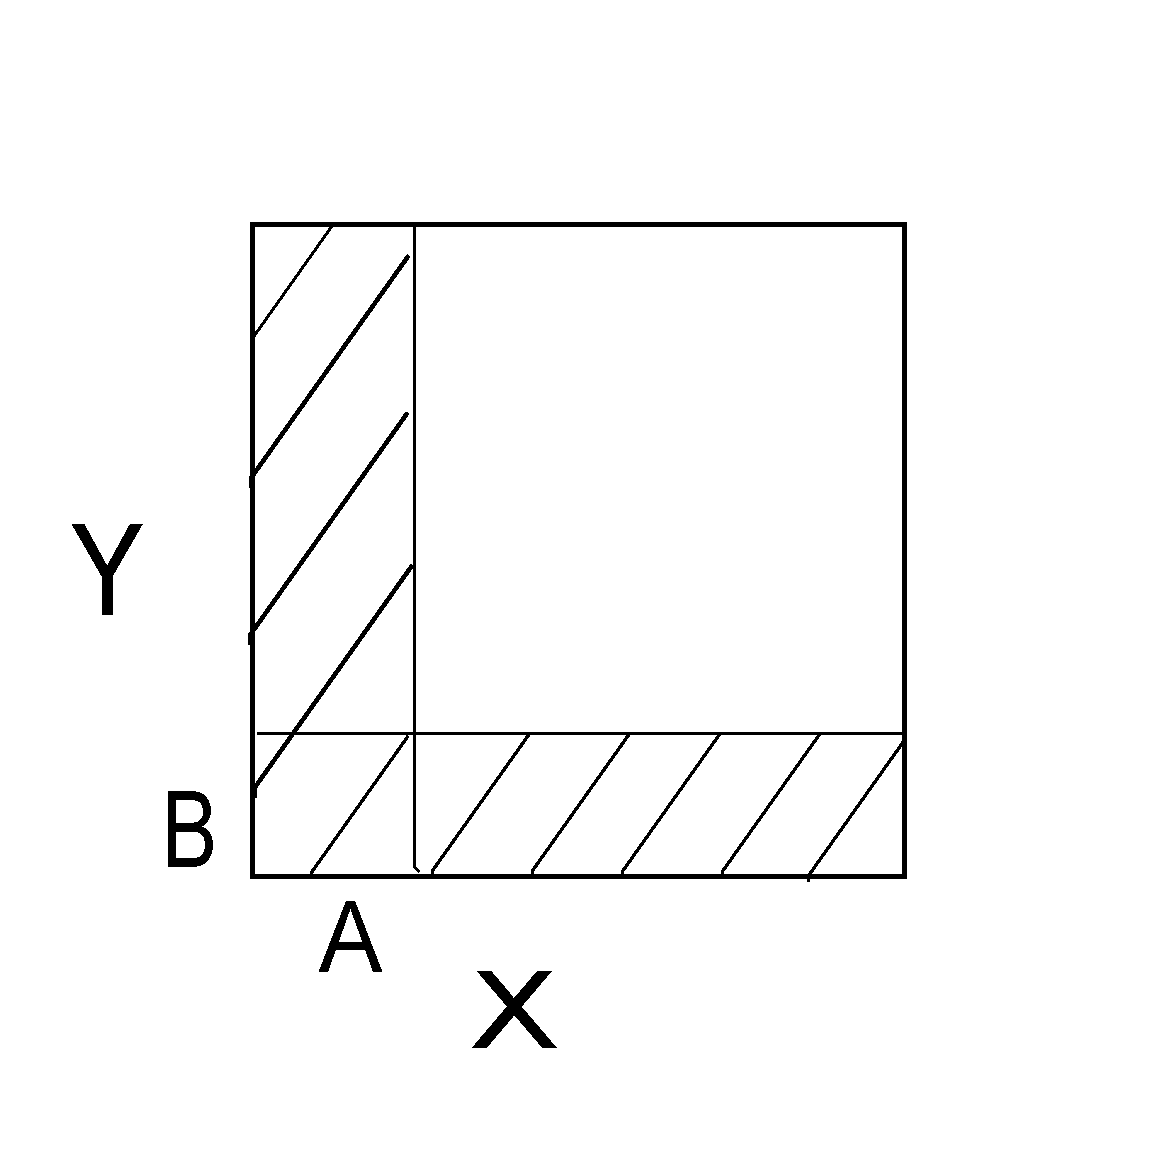
\includegraphics[width=0.2\textwidth]{figures/15.pdf}
\caption{\small Diagram of a relative product, for that last equality.}
\end{figure}

Now suppose $X = Y$; then we have a diagonal map $\Delta: (X, A \cup B) \to (X \times X, X \times B \cup A \times X)$ which induces a relative cup product:
\begin{ctikzcd}
K(X, A) \otimes K(X, B)\dar[equal] \rar["\smile"] & K(X, A \cup B) \\
\Ktwee(X/A) \otimes \Ktwee(X/B) \rar & K(X \times X, X \times B \cup A \times X)\uar["\Delta^*"]
\end{ctikzcd}
When $A \simeq \ptspace \simeq B$ we obtain
\begin{ctikzcd}
K(X, A) \otimes K(X, B)\dar[equal] \rar["\smile"] & \Ktwee(X,A\cup B)\rar &\Ktwee(X)\\
\Ktwee(X) \otimes \Ktwee(X) \rar & \Ktwee(X\sprod X)\uar["\Delta^*"]
\end{ctikzcd}
Where the map $\Ktwee(X,A\cup B)\to \Ktwee(X)$ is pulling back along the inclusion $(X,\ptspace)\to (X,A\cup B)$. This composite map $\Ktwee(X)\otimes \Ktwee(X)\to \Ktwee(X)$ is the product on reduced $K$ theory.
If in addition $A \cup B = X$, we get $K(X, A \cup B) = 0$, so the smash product map is trivial.  We have shown
\begin{lem}
If $X = A \cup B$ and $A \simeq \ptspace \simeq B$, then $\Ktwee(X)^2 = 0$; e.g., any suspension has this property.
\end{lem}
\begin{lem}
For all $n$, $K(S^{2n})=\Z[x_n]/x_n^2$, and $\psi^k(x_n)=k^nx_n.$
\end{lem}
\begin{proof}
\noindent By the previous lemma, $\Ktwee S^2 = \Z \langle \bundle{L} - 1 \rangle$ is subject to the relation $(\bundle{L} - 1)^2 = 0$.  So $K(S^2) = \Z[x_1]/x_1^2$. Now $\bundle{L}$ is a line bundle, so $\psi^k (\bundle{L}) = \bundle{L}^k$.  Thus
\[\psi^k(x)  = \psi^k(\bundle{L} - 1) = \bundle{L}^k - 1=(1+x_1)^k-1=kx_1.\]
By Bott, again, we have $\Ktwee(S^{2n}) \stackrel{\cong}{\from} \Ktwee(S^2)^{\otimes n}$, sending $x^{\otimes n}$ to $x_n=x_1^{\wedge n}$, so $K(S^{2n}) \cong \Z[x_n]/x_n^2$.

By lemma \ref{smashprodcommadams},
$\psi^k(x_n) = \psi^k(x_1^{\wedge n}) = \psi^k(x_1)^{\wedge n} = (kx_1)^{\wedge n} = k^n x_n$.
\end{proof}
\noindent
In particular, the Adams operations detect the dimension of an even-dimensional sphere!

\begin{wrapfigure}{r}{0.3\textwidth}
\centering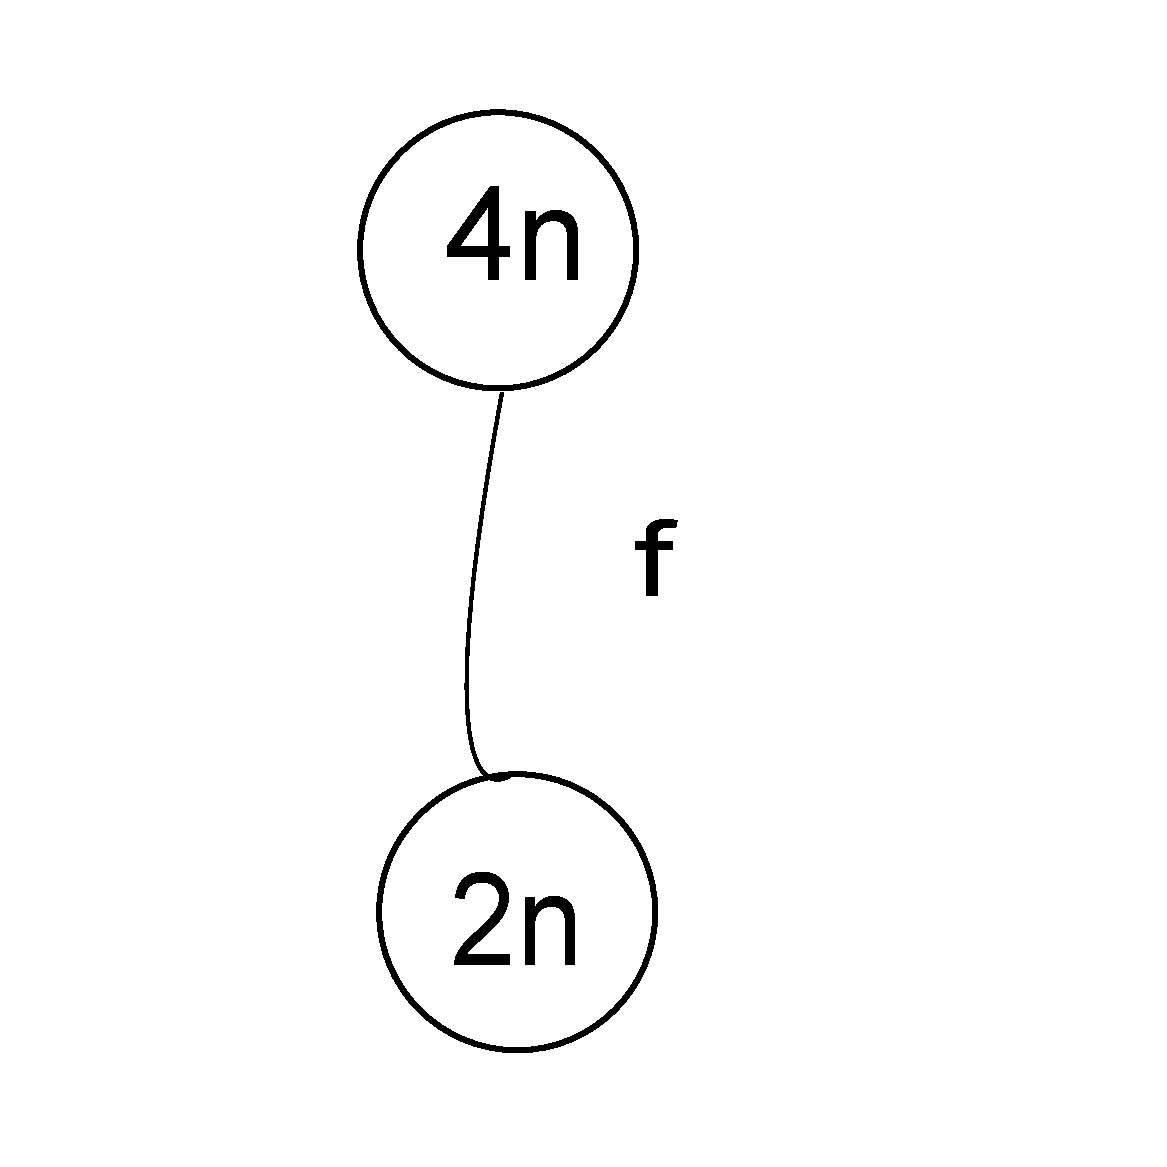
\includegraphics[width=0.2\textwidth]{figures/16.pdf}
\caption{\small Set-up for the Hopf invariant 1 problem.}
\end{wrapfigure}
OK, so now we can use all this equipment to prove that Hopf-invariant 1 problem. That is, we want to show that there is no element of Hopf invariant one in $\pi_{4n-1}(S^{2n})$ for $n\neq1,2,4$. Remember the set up:
\begin{ctikzcd}
S^{4n-1}\rar["f"] & S^{2n} \rar["i"] & X \rar["k"] & S^{4n}
\end{ctikzcd}
Here, $k$ is obtained by collapsing $X=C(f)$ onto its $4n$-cell, i.e.\ by continuing the cofiber sequence. As $f$ is 0 in $K$-theory, the long exact sequence obtained from the cofiber sequence $S^{2n}\to X\to S^{4n}$ degenerates into a short exact sequence of reduced $K$-groups, which splits $\Ktwee(X)$ into $\Z\langle x\rangle\oplus\Z\langle y\rangle$ (as $\Ktwee(S^{2n})$ is free):
\begin{ctikzcd}[row sep=0em]
0&\lar\Ktwee(S^{2n})&\lar["i^*"]\Ktwee(X)&\lar["j^*"]\Ktwee(S^{4n})&\lar0\\
 & x_n & \lar[mapsto]x \\
 && y  & \lar[mapsto] x_{2n}
\end{ctikzcd}
%So there is an $x \in \Ktwee(X)$ such that it pulls back to $x_n$.
Now $y^2=j^*(x_{2n})^2=0$, $i^*(x^2)=x_n^2=0$ and $i^*(xy)=x_n\cdot0=0$. Thus, for some $a,b\in\Z$, we have
\[K(X)=\Z\langle1,x,y\rangle\text{ with multiplication }y^2=0,\ x^2=ay,\ xy=by.\]
%In addition, $\Ktwee(X) \stackrel{j^*}{\from} \Ktwee(S^{4n})$ is injective, so $y^2 = j^* x_{2n}^2 = 0$.  This $K(X)$ has three generators, $\langle 1, x, y \rangle$, and the relations $y^2 = 0$, $x^2 = ay$.  ($x^2 = ay + bx$, but $b = 0$ since $0 = x_n^2 = i^* x^2 = b x_n$.)
\begin{claim}
$a$ is the Hopf invariant.
\end{claim}
\begin{proof}
There are a variety of ways to justify this claim; for example, you could use the Chern character, which provides a ring homomorphism $K(X) \to H^*(X; \Q)$.  Also the Atiyah-Hirzebruch spectral sequence works nicely: $E_2^{s, t} = H^s(X; K^t(\ptspace)) \Rightarrow K^*(X)$.  $X$ is very simple, so we can write this down easily:
\[E_2^{s,t}=0\text{ unless $t$ is even and $s=0,2n,4n$, otherwise $E_2^{s,t}\equiv\Z$.}\]
In particular, as every nonzero entry has even total dimension, there can be no differentials, and the spectral sequence collapses by $E_2$ page. In particular, we can identify the $E_2$ and $E_\infty$ pages.

Let $1\in H^{0}(X;K^0(\ptspace))$, $u\in H^{2n}(X;K^0(\ptspace))$ and $v\in H^{4n}(X;K^0(\ptspace))$ be generators. Then, if $p\in K^{-2}(\ptspace)$ is the periodicity element, $E_2^{2n,-2n}=\Z\langle p^nu\rangle$ and $E_2^{4n,-4n}=\Z\langle p^{2n}v\rangle$.
Now the total degree zero line computes $K(X)$, so that
\[K(X)=
\Z\langle1\rangle\oplus
\Z\langle p^nu\rangle\oplus
\Z\langle p^{2n}v\rangle\]
Now because the product on the $E_\infty$ page is induced by that on $K^*(X)$, we must have $(p^nu)\cdot(p^nu)=\pm a(p^{2n}v)$, and thus $u\cdot u=\pm av$. Finally, the product structure on $E_2^{*,0}$ is just the normal cup product structure of $H^*(X)$, showing that $a$ is the Hopf invariant.
%
%But everything in the $E_2$ term happens in even dimensions, so there are no differentials.  And since the spectral sequence is nice with respect to all the algebraic structure in sight, clearly the $x$ and $y$ represent the generators of $\Ktwee(X)$, and $a = H(f)$.
\end{proof}
\begin{thm}
The Hopf invariant $a$ cannot be odd unless $n = 1, 2, 4$.
\end{thm}
\begin{proof}
We'll start by assuming that $a$ is odd.
Firstly, for each $k$, $i^*(\psi^k(x))=\psi^k(x_n)=k^nx_n$. Moreover, $\psi^k(y)=\psi^k(j^*(x_{2n}))=j^*(\psi^kx_{2n})
=j^*(k^{2n}x_{2n})=k^{2n}y$. Thus, for some $b_k\in\Z$:
\[\psi^k(x)=k^nx+b_ky;\textup{ \ and \ }\psi^k(y)=k^{2n}y.\]
Now using lemma \ref{frobeniuslemma}, and writing $\equiv$ for congruence mod 2:
\[0\not\equiv ay=x^2\equiv\psi^2(x)=2^nx+b_2y.\]
Examining $y$ coefficients, we see that $b_2$ must be odd. Now we calculate:
\begin{align*}
\psi^3 \psi^2(x) & = \psi^3(2^n x + b_2 y) = 2^n(3^n x + b_3 y) + b_2 3^{2n} y, \\
\psi^2 \psi^3(x) & = \psi^2(3^n x + b_3 y) = 3^n(2^n x + b_2 y) + b_3 2^{2n} y.
\end{align*}
Again examining $y$ coefficients gives an equation $b_3(2^{2n} - 2^n) = b_2(3^{2n} - 3^n)$.  $2^n$ divides the left hand expression, and $b_2$ is odd, so $2^n$ must divide $3^n - 1$. The result follows from the next claim.
\end{proof}
\begin{claim}
$2^n$ can only divide $3^n - 1$ when $n=1,2,4$.
\end{claim}
\begin{proof}
Writing $\nu(m)$ for the largest number $r$ such that $2^r$ divides $m$, so that $2^n|3^n-1$ iff $\nu(3^n-1)\geq n$. If one can prove the following formula, the result is immediate:
\[
\nu(3^n-1) = \begin{cases} 1 & \hbox{$n$ odd}, \\ \nu(n) + 2 & \hbox{$n$ even}.\end{cases}
\]
To make this calculation, we have the following argument, due to David Anick. For any $e\geq0$:
\begin{alignat*}{3}
3^{2e+1} - 1 &= 9^e \cdot 3 - 1 &&\equiv 2 \pmod 8,\textup{ \ so that \ }&\nu(3^\textup{odd} - 1)&=1;\\
3^{2e+1} + 1 &= 9^e \cdot 3 + 1 &&\equiv 4 \pmod 8,\textup{ \ so that \ }&\nu(3^\textup{odd} + 1)&=2;\\
3^{2e} + 1 &= \ \ 9^e + 1 &&\equiv 2 \pmod 8,\textup{ \ so that \ }&\nu(3^\textup{even} + 1)&=1.
\end{alignat*}
If $n$ is odd, we are done. Else, write $n=2^{\nu(n)}d$ for $d$ odd, and factorise:
\[
3^n-1=3^{2^{\nu(n)} d} - 1 = (3^d + 1) (3^d - 1) (3^{2d} + 1) \cdots (3^{2^{{\nu(n)}-1}d} + 1).
\]
We count exactly $2+1+1+\cdots+1=\nu(n)+2$ factors of two in this expression, as advertised.
\end{proof}

% >>>
\fi
\begin{SummaryNote}
\Bullet In $K(X)$, $\psi^p(x) \equiv x^p \pmod{p}$  for $p$ prime.

\Bullet The dashed external smash product is induced by the solid vertical morphisms in the following diagram. It commutes with Adams operations. The lower short exact sequence appears because $X\vee Y\to X\times Y$ splits after one suspension.
\begin{ctikzcd}[column sep=small]
0\ar[r] & \Ktwee(X) \otimes \Ktwee(Y)\rar[r] \dar[dashed,"\wedge"]& K(X) \otimes K(Y)\rar["\alpha"]\dar["\times"]&\Ktwee(X) \oplus \Ktwee(Y) \oplus \Z\dar[equal]\rar&0\\
0\ar[r]&\Ktwee(X \sprod Y)\rar["c^*"]&K(X\times Y)\ar[r]&K(X\vee Y)\ar[r]&0
\end{ctikzcd}

\Bullet Products on $K(X)$ vanish if $X$ is the union of contractible subsets (e.g.\ $X=S^{n}$).

\Bullet  $K(S^{2})=\Z[x_1]/x_1^2$. Since $x_1+1$ is a line bundle, $\psi^k(x_1)=(x_1+1)^k-1=kx_1$.


\Bullet For all $n$, $K(S^{2n})=\Z[x_n]/x_n^2$, and $\psi^k(x_n)=k^nx_n$, as the smash product map commutes with $\psi^k$. Thus the Adams operations detect the $n$ in $S^{2n}$!%dimension of an even-dimensional sphere!

\Bullet This all comes together to prove Hopf invariant one.
\end{SummaryNote}


\newcommand{\HopfDiagram}[6]{
    %#1: left  bar color -> green
    %#2: right bar color -> green
    %#3: accepts: BlackBeard;
    %             WhiteBeard;   Any of these three will produce SZ,
    %             ArrowBeard;     with various colourings of the arrows
    %#4: x-offset
    %#5: y-offset
    %#6: accepts: cone;         Includes the cone on X*Y
    %             nojoin;       Does not display any X or Y
    %             BottomBar
    %             LeftBar
    \ifthenelse{\equal{#1}{on}}
    {\colorlet{LeftBar}{green}}
    {\colorlet{LeftBar}{black}}
    \ifthenelse{\equal{#2}{on}}
    {\colorlet{BottomBar}{green}}
    {\colorlet{BottomBar}{black}}
    \ifthenelse{\equal{#1}{on}\OR \equal{#2}{on}}
    {\colorlet{TheDot}{green}}
    {\colorlet{TheDot}{black}}
    \ifthenelse{\equal{#3}{BlackBeard}}
    {\colorlet{GlueColor}{black}}
    {\colorlet{GlueColor}{red}}
    \ifthenelse{\equal{#3}{WhiteBeard}}
    {\colorlet{GlueColor}{white}}
    {}

    \ifthenelse{\equal{#6}{cone}}
    {\foreach \i in {0,...,9}
    {\draw (#4+0,.1*\i+#5) -- (#4+1-.1*\i,1+#5);}
    \foreach \i in {1,...,9}
    {\draw (#4+.1*\i,0+#5) -- (#4+1,1-.1*\i+#5);}
    \draw (#4+1,0+#5) -- (#4+1,1+#5);
    \draw (#4+0,1+#5) -- (#4+1,1+#5);
    }{}

    \ifthenelse{\equal{#3}{WhiteBeard}}{}
    {
    \ifthenelse{\equal{#6}{nojoin}}{}
    {
    \ifthenelse{\equal{#6}{BottomBar}}{}
    {\draw[ultra thick,LeftBar] (#4+0,0+#5) -- (#4+0,1+#5);}
    \ifthenelse{\equal{#6}{LeftBar}}{}
    {\draw[ultra thick,BottomBar] (#4+0,0+#5) -- (#4+1,0+#5)};
    \fill[TheDot] (#4+0,0+#5) circle (3.42pt);
    }
    }

    \ifthenelse{\equal{#3}{ArrowBeard}\OR \equal{#3}{BlackBeard}\OR \equal{#3}{WhiteBeard}}
    {
    \ifthenelse{\equal{#6}{BottomBar}}{}
    {\draw[ultra thick,LeftBar] (#4+-.5,-.5+#5) -- (#4+-.5,1+#5);}
    \ifthenelse{\equal{#6}{LeftBar}}{}
    {\draw[ultra thick,BottomBar] (#4+-.5,-.5+#5) -- (#4+1,-.5+#5);}
    \fill[TheDot] (#4+-.5,-.5+#5) circle (3.4pt);
    \foreach \i in {0,2,4,6,8,10}
    {\draw[->,GlueColor] (#4+-.1+.11*\i,-.1+#5) -- (#4+-.4+.14*\i,-.4+#5);}
    \foreach \i in {2,4,6,8,10}
    {\draw[->,GlueColor] (#4+-.1,-.1+.11*\i+#5) -- (#4+-.4,-.4+.14*\i+#5);}
    }{}%end \foreach then end \ifthenelse
} 

\section{The James construction} % <<<
\label{TheJamesConstruction}
\ifx\OutputTheJamesConstruction\undefined\else
First, remember the group $J(X)$.  This was the quotient of $KO(X)$ by the equivalence generated on the level of bundles by $V \simeq_J W$ if and only if $S(V \oplus n \varepsilon) \simeq_\textup{f.h.e.} S(W \oplus n \varepsilon)$.  An immediate consequence of the vector field problem is:\footnote{Note that theorem \ref{KOtoJofRPm} is part of theorem \ref{AdamsKORPn} (Adams), and theorem \ref{AdamsKORPn} solves the vector field problem.}
\begin{ConfusedNote}
\textbf{Is this the point?}
Suppose that it is known that $\widetilde{KO}(\RP^m)\simeq\Z/a_m\Z$, and that it is generated by $[\bundle{L}]-1$ (this is the first part of theorem \ref{AdamsKORPn}). Then we can prove the rest of theorem \ref{AdamsKORPn} (i.e.\ theorem \ref{KOtoJofRPm}) using the discussion in lecture \ref{UsingTheSquaresAndThomSpaces}. Recall that theorem \ref{AdamsKORPn} implies the solution of the vector fields problem.
\begin{thm} \label{KOtoJofRPm}
The surjection $\widetilde{KO}(\RP^m) \onto \widetilde J(\RP^m)$ is an isomorphism.
\end{thm}
\begin{proof}
$n(\bundle{L} - 1) \mapsto 0$ means $n \bundle{L}$ is stably fiber homotopy trivial; this implies a (stable) splitting:
%\begin{ctikzcd}
%\RP^{m+n}_n \rar & S^n \\
%S^n\uar\urar["simeq"]
%\end{ctikzcd}
But we know from lecture \ref{UsingTheSquaresAndThomSpaces} that this implies that $\nu(n)\geq m+1$, and since $m\geq \varphi_m$, $a_k=2^{\varphi_m}$ divides $n$, so $n(\bundle{L} - 1)$ was already zero in $\widetilde{KO}(\RP^m)$.\footnote{Homework: compute $\widetilde J(S^n)$.}
\end{proof}
\end{ConfusedNote}

Relations to problems in unstable homotopy are often mediated by the EHP sequence, so the next topic will be to construct it.  Our starting point will be a theorem of Bott and Samelson about $H_*(\Loops \Suspend X)$; for a proof see Whitehead~\cite{Whitehead}.  There is a map $\alpha: X \to \Loops \Suspend X$ which embeds $X$ as the ``straight loops'': $\alpha$ is adjoint to $\textup{Id}_{\Sigma X}$, and sends $x\in X$ to the loop $t\mapsto [t,x]$.
%\begin{figure}[h!]
%\centering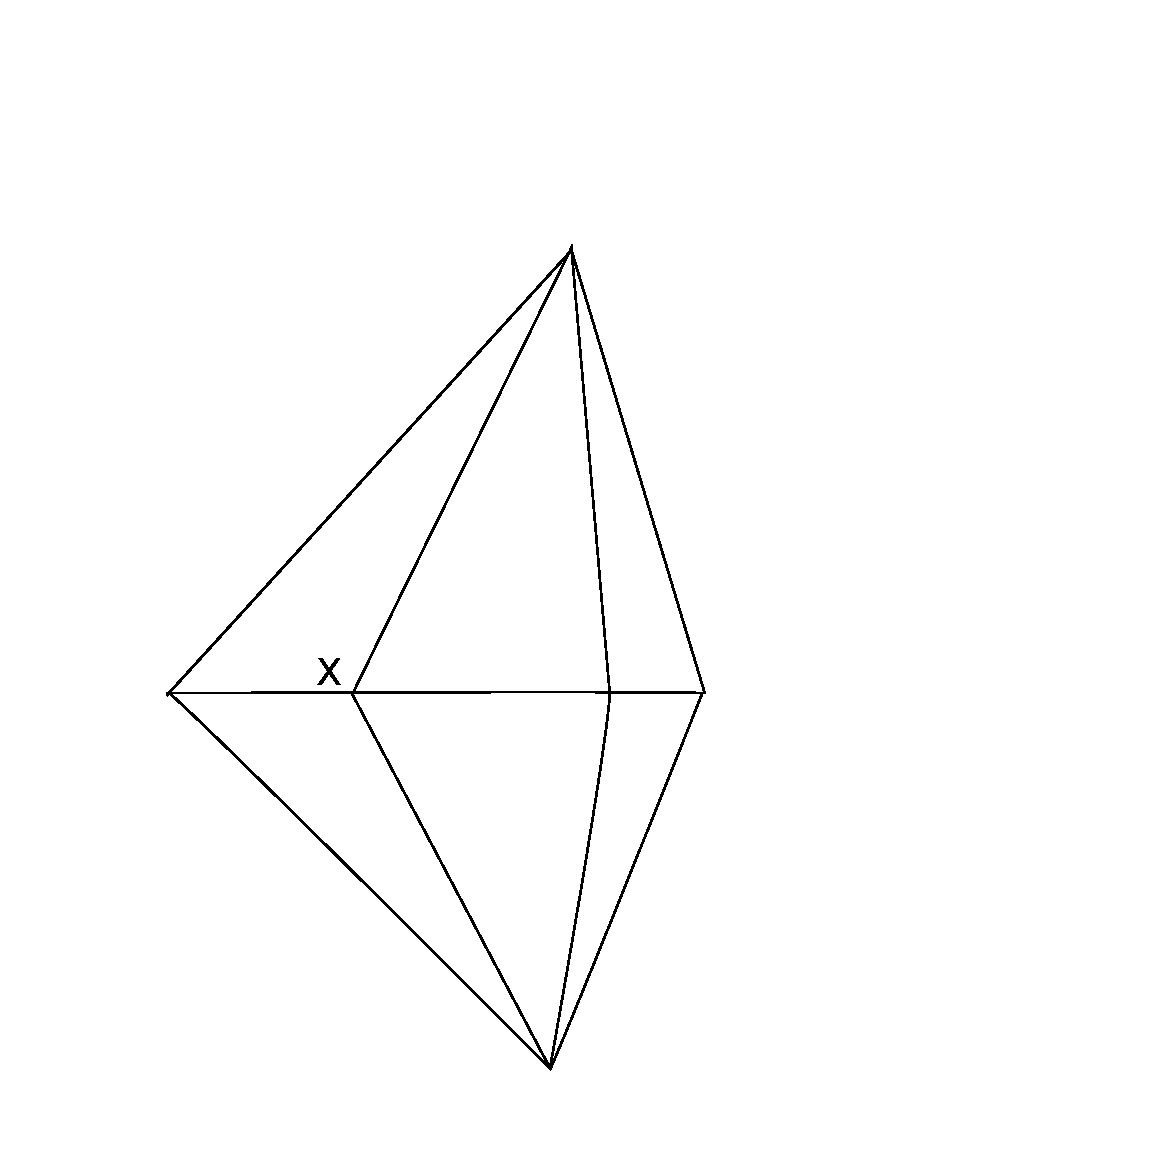
\includegraphics[width=0.3\textwidth]{figures/17.pdf}
%\caption{\small The image of $x$ under $\alpha$.}
%\end{figure}
Choose a coefficient ring $R$.
The loop structure makes $H_* (\Loops \Suspend X)$ into an algebra, so $\alpha_*: \Htwee_*(X) \to H_* (\Loops \Suspend X)$ yields a unique extension to the tensor algebra $\T(\Htwee_*(X;R))$ on the $R$-module $\Htwee_*(X;R)$ (here, tensor products are over $R$):
\begin{ctikzcd}
\T(\Htwee_*(X;R))\rar["\overline\alpha"]&H_*(\Omega\Sigma X;R)\\
\uar[equal]\bigoplus_{k\geq0}\Htwee_*(X;R)^{\otimes k}& \Htwee_*(X;R)\lar[hook']\uar["\alpha_*"']
\end{ctikzcd}
%
\begin{thm}
If $X$ is connected, $R$ is a principal ideal domain, and $H_*(X; R)$ is torsion-free, then $\T(\Htwee_*(X; R)) \stackrel{\overline \alpha}{\to} H_*(\Loops \Suspend X; R)$ is an isomorphism.
\end{thm}
Now since $H_*(X; R)$ is torsion-free:
\[\bigoplus_{k \ge 0} \Htwee_*(X;R)^{\otimes k} \cong \bigoplus_{j \ge 0} \Htwee_* (X^{(k)};R) \cong \Htwee_*{\left(\textstyle\bigvee_{k \ge 0} X^{(k)};R\right)},\]
so you might hope idealistically that $\Suspend \Loops X$ splits as a wedge of smash powers of $X$.  Of course that's not true, but amazingly enough, it \emph{does} split after one suspension:
\begin{thm}[James, probably]
When $X$ is a connected CW-complex, there is a homotopy equivalence
\[
\Suspend \Loops \Suspend X \simeq \bigvee_{k \ge 1} \Suspend X^{(k)}
.\]
Moreover, this equivalence realises the isomorphism $\overline\alpha$ above.
\end{thm}
\begin{proof}[Proof sketch. \textbf{Come back to this!}]
First, as $X$ is connected, $\Suspend X^{(k)}$ and $\Suspend \Loops \Suspend X$ are simply connected.  If we produce a map giving an isomorphism in homology, then by the Hurewicz theorem we have a weak equivalence.  Then if you believe that both spaces are CW-complexes and some version of the Whitehead theorem, then we're done.

Now, $[\bigvee_{k \ge 1} \Suspend X^{(k)}, \Suspend \Loops \Suspend X]_* = \prod_{k \ge 1}[\Suspend X^{(k)}, \Suspend \Loops \Suspend X]_*$, which is to say that the wedge is the coproduct in the category of pointed spaces and homotopy classes of maps.  So we construct a map on $\Suspend X^{(k)}$ for $k \ge 1$:
\begin{ctikzcd}
\Suspend X^{(k)} \rar["(1)"'] & \Suspend X^k \rar["(2)"',"\Suspend \alpha^k"] & \Suspend(\Loops \Suspend X)^k \rar["(3)"',"\Suspend \mu"] & \Suspend \Loops \Suspend X.
\end{ctikzcd}
\begin{enumerate}
\item We've seen this before in the case $k = 2$: we produced a map
\begin{ctikzcd}[column sep=large]
\Suspend (X \times Y) \rar["\textup{pinch}"] & \Suspend (X \times Y) \wsum \Suspend(X \times Y) \rar["\Suspend(pr_1 \wsum pr_2)"] &[1.3em] \Suspend X \wsum \Suspend Y \\
\Suspend(X\vee Y)\uar[hook]\urar["\simeq"]
\end{ctikzcd}

On the other hand the sequence $\Suspend(X \wsum Y) \to \Suspend(X \times Y) \to \Suspend(X \sprod Y)$ combines to provide
\begin{ctikzcd}
\Suspend(X \wsum Y)\dar["\simeq"'] \rar & \Suspend(X \times Y)\dar \rar & \Suspend(X \sprod Y)\dar["\simeq"'] \\
\Suspend X \wsum \Suspend Y \rar & \Suspend(X \sprod Y) \wsum \Suspend X \wsum \Suspend Y \rar & \Suspend(X \sprod Y)
\end{ctikzcd}
The two horizontal lines give exact sequences in homotopy, so by the five lemma and assuming $X$ and $Y$ are CW-complexes, we get a map going back, $\Suspend(X \sprod Y) \wsum \Suspend X \wsum \Suspend Y \to \Suspend (X \times Y)$.  Now the composite $\Suspend(X \sprod Y) \to \Suspend(X \sprod Y) \wsum \Suspend X \wsum \Suspend Y \stackrel{\simeq}{\to} \Suspend(X \times Y)$ gives the first map $\Suspend X^{(k)} \to \Suspend X^k$ in the overall diagram; from its construction we see that it splits the homology of $\Suspend X^k$ as a sum $H_* \Suspend X^{(k)} \oplus H_* ((\Suspend X)^{\wsum k})$ \textbf{incorrect expression}.
\item The second map in the overall diagram is the suspension of the ``straight loops'' embedding that spawned this whole discussion, repeated $k$ times.
\item The third map in the overall diagram is the suspension of the loop multiplication map.  Note that loop multiplication is not strictly associative due to parameterization problems, but it is associative up to homotopy.
\end{enumerate}
Now the Bott-Samelson theorem says that the product of these composities as $k$ ranges over the positive integers is an isomorphism in homology.
\end{proof}

Now note that the Bott-Samelson theorem required that $H^*(X; R)$ be torsion-free and $R$ a principal ideal domain.  However, the claim is that this theorem of James holds for arbitrary coefficients, in particular with $\Z$-coefficients; in fact, we have a general proposition:
\begin{lem}
If $X \to Y$ induces an isomorphism on homology $H_*(X; F) \stackrel{\cong}{\to} H_*(Y; F)$ for $F$ either $\Z/(p)$ or $\Q$, then $H_*(X; \Z) \stackrel{\cong}{\to} H_*(Y; \Z)$.
\end{lem}
\begin{proof}
Use the universal coefficient theorem many times.  First, for any $p$, $f$ induces a map of long exact sequences induced by the short exact sequence
\begin{ctikzcd}
0 \rar & \Z/(p) \rar & \Z/(p^2) \rar & \Z(p) \rar & 0
\end{ctikzcd}
of coefficients. By the five lemma, $H_*(f;\Z/(p^2))$ is an isomorphism. Similarly, using induction on $n$,
\begin{ctikzcd}
0 \rar & \Z/(p^n) \rar & \Z/(p^{n+1}) \rar & \Z/(p) \rar & 0
\end{ctikzcd}
shows that $H_*(f;\Z/(p^n))$ is an isomorphism for all $n$.

Now the limit $\Z_{p^\infty} = \cdots \into \Z/(p^n) \into \Z/(p^{n+1}) \into \cdots = \bigcup \Z/(p^n)$ is called the ``Pr\"ufer group''. As homology commutes with direct limits, $H_*(f;\Z_{p^\infty})$ is an isomorphism.  Finally, as $\Q/\Z \cong \bigoplus \Z_{p^\infty}$, the sum being taken over all primes $p$,\footnote{View the Pr\"ufer group $\Z_{p^\infty}$ as the quotient in the short exact sequence $0 \to \Z \to \Z[1/p] \to \Z[1/p]/\Z \to 0$. Define a map $\Q\to\Z_{p^\infty}$ by $a/b+c/p^d\mapsto c/p^d$ whenever $b$ is coprime to $p$. Now note that the induced map $\Q\to\prod\Z_{p^\infty}$ factors through the inclusion of $\bigoplus\Z_{p^\infty}$, that this factorisation is surjective, and that it has kernel $\Z$.}
we are done.
\end{proof}

Now the proof of the James' Theorem relied on some heavy stuff: Bott-Samelson, the Hurewicz theorem, and the JHC Whitehead theorem.  You may think that's too slick, and you would be right, because we skipped over the ``James construction.''  The biggest difficulties above were caused by the nonassociativity of loop composition.  The idea is to replace $\Loops X$ with a homotopy equivalent space, the ``Moore loops,'' where composition is associative.

The space of ``Moore loops'' on $X$ is simple: since scaling caused trouble, don't scale!  A Moore loop is a map $\omega: [0, T] \to X$, $T \ge 0$, with $\omega(0) = \omega(T) = *$.  Loop multiplication of a Moore loop $\omega: [0, T] \to X$ and another Moore loop $\tau: [0, S] \to X$ gives a loop $\tau \cdot \omega: [0, T + S] \to X$.  We'll call this space $\Loops X$ too.  It comes with a basepoint $*$, the path of length 0, and has a strictly associative product with a strict unit *.  We get a map $\alpha: X \to \Loops \Suspend X$ in the same way. The old $\Omega X$ embeds in the Moore loops $\Omega X$ as the subspace of paths with length 1.

Now $\alpha$ factors
\begin{ctikzcd}[column sep=tiny]
X \ar[rr,"\alpha"]\drar & & \Loops \Suspend X \\
& \urar["\tilde \alpha"'] J(X)
\end{ctikzcd}
through the space $J(X)$,\footnote{``J'' for ``James''.} the ``free monoid'' on $X$:
\[
J(X) = \coprod_{k \ge 0} X^k / \sim,
\]
where $\sim$ is generated by $x \cdot * = x$.  And the ``real'' theorem is:
\begin{thm}
When $X$ is a connected CW complex, $\tilde \alpha$ is a homotopy equivalence.
\end{thm}
Notice that this gives a map back, and so a way of constructing maps out of a loop space.  In general, this is hard to do; adjointness is no help for maps \emph{out} of a loop space.  For example, $J(X)$ is filtered by $J_n = \coprod_{j \le n} X^k / \sim$, and we fill out the following commutative diagram with the obvious maps:
\begin{ctikzcd}[column sep=small]
X^n\rar\ar[rrrd,start anchor=south east] & J_n(X)\rar & J_n(X)/J_{n-1}(X) \rar[equal] & X^n/F_{n-1}X^n\dar[equal]\\
&&& X^{(n)}
\end{ctikzcd}
%
On the other hand, suspending once we get
\begin{ctikzcd}
\Suspend X^{(n)} \rar\ar[dd,"\text{split map}"'] & \Suspend \Loops \Suspend X \\
&\Suspend J(X)\uar["\simeq"]\\
\Suspend X^n\rar & \Suspend J_n(X)\uar\rar &\Suspend X^{(n)}
\end{ctikzcd}
so after one suspension $J_n(X)$ splits as $\Suspend J_n(X) \simeq \bigvee_{k \le n} \Suspend X^{(k)}$.

\textbf{Everything above here should be rewritten}

Finally, notice that we have a map $\hhat_m$:
\begin{ctikzcd}
\bigvee_{\!k \ge 0} \Suspend X^{(k)} \dar["\Suspend(\text{collapse})"'] \rar["\simeq",yshift=0.25em] & \lar["\exists",yshift=-0.25em] \Suspend \Omega \Suspend X\dlar["\hhat_m"] \\
\Suspend X^{(m)}
\end{ctikzcd}
Its adjoint $h_m: \Loops \Suspend X \to \Loops \Suspend X^{(m)}$ is called the $m$th (James-)Hopf invariant.  When $X = S^n$ and $m = 2$, we have the map:
\[h_2:\Loops S^{n+1} \to \Loops \Suspend (S^n)^{(2)} = \Loops S^{2n+1}.\]
%; then $h_2$ is a map $\Loops S^{n+1} \to \Loops \Suspend (S^n)^{(2)} = \Loops S^{2n+1}$.
This is a piece of the EHP sequence; the rest comes from taking the homotopy fiber and looking at the long exact sequence in homotopy. To compute $H_n (\Loops S^{n+1})$, we use Bott-Samelson:
\[H_* (\Loops S^{n+1}) = \Trm(\Htwee_* (S^n)) = \Trm[u_1]\text{ \ where $|u_1| = n$. }\]
So $h_2$ induces a degree preserving map $\Trm[u_1] \to \Trm[u_2]$, which consequentially cannot be an algebra map.  We'd better try cohomology.

\ConfusedBox{
The following has become some kind of aside:

Alternatively, to compute $H_n(\Omega S^{n+1})$, you could use the path fibration $\Loops S^{n+1} \to PS^{n+1} \to S^{n+1}$, $(n > 0)$, and the Serre spectral sequence gives... (draw it).

\textit{Note that if you try to remember grading then $u^2 = (-1) u u$ for $u$ odd, so you lose commutativity by trying to remember grading, which is the reverse somehow of the usual situation. \textbf{I don't really get this.}}
}
\begin{thm}\label{ThmAlgStrucLoopsSphere}
With coefficients in a principal ideal domain \textup{\textbf{(should this say `field'?)}}, there are isomorphisms:
\begin{alignat}{2}
H^* (\Loops S^{2n+1}) & \cong \Gamma[x_{2n}]&\qquad&\text{as Hopf algebras}, \label{FirstIsoEqn}\\
H^* (\Loops S^{2n}) & \cong \Lambda[x_{2n-1}] \otimes \Gamma[x_{4n-2}]&&\text{as algebras}, \label{SecondIsoEqn}\\
H_* (\Loops S^{2k}) & \cong H_*( S^{2k-1}) \otimes H_* (\Loops S^{2k-1})&&\text{as coalgebras, not as algebras.}\label{ThirdIsoEqn}
\end{alignat}
Here, $\Gamma$ stands for the divided polynomial algebra.
\end{thm}
We digress a bit to explain the theorem statement.  First, there is always a diagonal map $\Delta: X \to X \times X$.  Assuming that $X$ is nice enough (or that the coefficients are nice enough), the external product $H_*(X) \otimes H_*(X) \to H_*(X \times X)$ is an isomorphism, so there's a map going backwards as well.  We call the composite of $\Delta_*$ with this inverse map a ``coproduct'', denoted $\Delta$:
\begin{ctikzcd}
H_*(X)\ar[rd,"\Delta_*"']\ar[rr,"\Delta"] &&H_*(X)\otimes H_*(X)\ar[ld,"\cong"]\\
&H_*(X\times X)
\end{ctikzcd}
The coproduct map $\Delta$, along with the obvious map $H_* (X) \to R= H_* (\ptspace)$ gives $H_* (X)$ the structure of a coalgebra.

What is a coalgebra?  Well, you reverse the diagrams for an algebra; i.e., you have maps $\Delta: C \to C \otimes_R C$ and $\epsilon: C \to R$ satisfying coassociativity, counitality, and cocommutativity, corresponding to the following three diagrams:
\begin{cjointikzcd}[diagram sep=1.5em]
\diagram
    C \rar["\Delta"] \dar["\Delta"'] & C \otimes_R C \dar["\Delta \otimes 1"]\\
    C \otimes_R C \rar["1 \otimes \Delta"] & C \otimes_R C \otimes_R C
\diagram[3]
    & C\dlar["\cong"']\drar["\cong"]\dar["\Delta"'] \\
    R \otimes_R C & \lar["\epsilon \otimes 1"'] C \otimes_R C \rar["1 \otimes \epsilon"] & C \otimes_R R
\diagram[5em]
    &[-2em]C\dlar["\Delta"']\drar["\Delta"] &[-2em] \\
    C\otimes_R C \ar[rr,"T"]&& C\otimes_R C
\end{cjointikzcd}
Here $T$ is the graded commutative twist map: on a homogenous element we have $T(x\otimes y)=(-1)^{|x||y|} y\otimes x$.

Suppose that $X$ is connected, so $H_0(X) = R$, and there's a well-defined class $1$ in $H_0(X)$.  Then if $x \in H_n(X)$ where $n > 0$, $\Delta x = 1 \otimes a + \cdots + b \otimes 1$, where any omitted terms have positive degree both in the left- and right-hand factor.  Then $a = b = x$ by the counit axiom.  If $H_p (X)$ vanishes for $p < n$, then $ \Delta x = 1 \otimes x + x \otimes 1$, and $x$ is called ``primitive.''  Note that $\Delta 1 = 1 \otimes 1$.  If $\Delta x=x\otimes x$, the element $x$ is called group-like.\footnote{This terminology comes from the example $R[G]$; see below.}

In the example of $\Loops X$, the $H$-space structure says that $\mu: \Loops X \times \Loops X \to \Loops X$ fits into the following two homotopy commutative diagrams:\footnote{Some people call this an associative $H$-space.}
\begin{cjointikzcd}
\diagram
\ptspace \times \Loops X \drar \rar & \Loops X \times \Loops X \dar["\mu"] & \dlar\lar \Loops X \times \ptspace \\
& \Loops X
\diagram
\Loops X \times \Loops X \times \Loops X \dar["\mu\times 1"']\rar["1 \times \mu"] & \Loops X \times \Loops X\dar["\mu"'] \\
\Loops X \times \Loops X \rar["\mu"] & \Loops X
\end{cjointikzcd}
Over field coefficients, this induces the diagram
\begin{ctikzcd}
H_*(Y) \otimes H_* (Y) \dar["\cong"]\rar["\psi"] & H_* (Y) \\
H_*(Y \times Y)\urar["\mu_*"']
\end{ctikzcd}
where the isomorphism is of coalgebras.  (We omit the proof; you have to think about what the tensor product of coalgebras ought to be.)  The map $\psi$ is called the Pontrjagin product.

What does this mean, though?  It means that $H_* (Y)$ is a Hopf algebra.  So what's a Hopf algebra?  Well, it's a bunch of structure.  We have maps $\eta: R \to H$ and $\mu: H \otimes H \to H$ that give $H$ an algebra structure and maps $\epsilon: H \to R$ and $\Delta: H \to H \otimes H$ that give $H$ a coalgebra structure.  In addition, $\eta$ and $\mu$ are coalgebra maps, so they give commutative diagrams of the form:
\begin{cjointikzcd}
\diagram
    H\otimes H \dar["\Delta\otimes\Delta"]\ar[dd,bend right=60,"\Delta_{H\otimes H}"'{yshift=-0.6em}]\rar["\mu"] & H\ar[dd]\\
    H\otimes H\otimes \mathrlap{H\otimes H}\dar["1\otimes T\otimes 1"]\\
    H\otimes H\otimes H\otimes H \rar["\mu\otimes\mu"] & H\otimes H]
%
\diagram
    H\otimes H \dar["\epsilon\otimes\epsilon"]\ar[dd,bend right=50,"\epsilon_{H\otimes H}"'{yshift=-0.4em}]\rar["\mu"] & H \ar[ddl,"\epsilon"] \\
    R\otimes R\dar\\
    R
%
\diagram
    &[-2em]R\dlar[equal]&[-2em]\\
    R \ar[rr,"\eta"]\dar["\Delta"]&&H\ular["\epsilon"]\dar["\Delta"]\\
    R\otimes R\ar[rr,"\eta\otimes\eta"] && H\otimes H
\end{cjointikzcd}
Now you can check that the commutativity of these diagrams implies that $\Delta$ and $\epsilon$ are algebra maps, so the symmetric conditions are equivalent.

Another important example of a Hopf algebra is the group algebra $R[G]$ for $R$ a ring and $G$ a group. As an $R$-module, $R[G]$ is free on $G$ considered as a set. The product is generated by $[g][h] = [gh]$.  The coalgebra structure is given by $\Delta[g] = [g \otimes g]$ and $\epsilon[g] = 1$ for $g \in G$.  Notice that this explains the terminology ``group-like.''  In fact, if $R$ is of characteristic zero, the set of group-like elements of $R[G]$ is exactly $G$.  The coalgebra structure enables us to recover the generators!

Turning to the Bott-Samelson theorem: if $X$ is connected, $R$ is a principal ideal domain, and $H_* (X)$ is torsion-free, the theorem gave us an algebra isomorphism $\Trm (\Htwee_n(X))  \cong H_* (\Loops \Suspend X)$.  Now that we have established that $H_n (\Loops \Suspend X)$ is a Hopf algebra, the natural question is what the Hopf algebra structure on $\Trm (\Htwee_* (X))$ ought to be in order to make the isomorphism a Hopf algebra map.  In particular, we need a coproduct map $\Delta: \Trm \to \Trm \otimes \Trm$.  It has to be an algebra map, so by the universal property of $\Trm$ all we need is a suitable map $\widetilde{\Delta}: \Htwee_*(X) \to \Trm \otimes \Trm$, whose extension $\Delta$ is a coproduct map:
\begin{ctikzcd}
\Trm(\Htwee_* (X)) \rar["\Delta"] & \Trm (\Htwee_* (X)) \otimes \Trm (\Htwee_* (X)) \\
\Htwee_* (X) \uar \rar["\widetilde{\Delta}"] & \Htwee_* (X) \otimes \Htwee_* (X)\uar
\end{ctikzcd}
It works out that $\widetilde{\Delta} x$ is the obvious thing. For $x \in \Htwee_n (X)$, the map $\widetilde{\Delta}$ is given by:
\[\Delta x = x \otimes 1 + \widetilde{\Delta} x + 1 \otimes x\]


Returning at last to theorem \ref{ThmAlgStrucLoopsSphere}, let's compute the coalgebra structure of $H_* (\Loops S^{n+1}) =\Trm[u_1]$:
\begin{alignat*}{2}
\Delta u_1 & = u_1 \otimes 1 + 1 \otimes u_1,&\qquad&\textup{(as there is no room for middle terms)} \\
\Delta u_1^k & = (u_1 \otimes 1 + 1 \otimes u_1)^k,&&\textup{(as $\Delta$ is an algebra map)}
\end{alignat*}
In particular, as the product in $\Trm[u_1]\otimes \Trm[u_1]$ is $(\mu\otimes\mu)\circ (1\otimes T\otimes1)$, where $T(a\otimes b)=(-1)^{|a||b|}(b\otimes a)$:
\begin{align*}
\Delta u_1^2&=(-1)^{0\cdot n}u_1^2\otimes1+(-1)^{0\cdot0}u_1\otimes u_1+(-1)^{n\cdot n}u_1\otimes u_1+(-1)^{n\cdot 0}\otimes u_1^2\\
&=u_1^2\otimes1+(1+(-1)^{n})(u_1\otimes u_1)+1\otimes u_1^2
\end{align*}
\begin{itemize}
\item When $n$ is even, we could go on to prove that $\Delta u_1^k = {\displaystyle\sum_{i + j = k}} \binom{i+j}{i} u_1^i \otimes u_1^j$.
\item When $n$ is odd, we get that $u_1^2$ is primitive. As $u_1^2$ has even degree:
\begin{align*}
\Delta u_1^{2k} & = \sum_{i+j=k} {\textstyle\binom{i+j}{i}} u_1^{2i} \otimes u_1^{2j}, \text{ \ and}\\
\Delta u_1^{2k+1} & = (\Delta u_1^{2k})(\Delta u_1) \\
& = \sum_{i+j=k} {\textstyle\binom{i+j}{i}} (u_1^{2i+1} \otimes u_1^{2j} + u_1^{2i} \otimes u_1^{2j+1}).
\end{align*}
\end{itemize}
So $H_* (\Loops S^{2k} )\cong H_*( S^{2k-1}) \otimes H_* (\Loops S^{4k-1})$ as coalgebras, though certainly not as algebras giving (\ref{ThirdIsoEqn}).

Now consider $H^* (\Loops S^{n+1})$.  With any coefficients, the group structure is
\[
H^q(\Loops S^{n+1}; R) = \begin{cases} R \langle z_i \rangle & q=ni\textup{ \,(for each $i\geq0$)}, \\ 0 & \mathrm{otherwise}. \end{cases}
\]
Now with field coefficients, let's compute the ring structure.  We can use in this case the pairing of cohomology and homology, so picking $n$ to be even to start, we get
\begin{alignat*}{2}
\langle z_i z_j, u_1^{i+j} \rangle & = \langle \Delta^*(z_i \otimes z_j), u_1^{i+j} \rangle&\qquad& \\
& = \langle z_i \otimes z_j, \Delta_* u_1^{i+j} \rangle \\
& = \left\langle z_i \otimes z_j, \sum_{i'+j'=i+j} {\textstyle\binom{i'+j'}{i'}} u_1^{i'} \otimes u_1^{j'} \right\rangle&&\text{\ (as $n$ is even)} \\
& = {\textstyle\binom{i+j}{i}} = \left\langle {\textstyle\binom{i+j}{i}} z_{i+j}, u_1^{i+j} \right\rangle,
\end{alignat*}
In particular, $z_i z_j = \binom{i+j}{i} z_{i+j}$. This algebra is called the divided polynomial algebra on $z_1$, denoted $\Gamma[z_1]$, and we get $H^* (\Loops S^{2k+1}) \cong \Gamma[x_{2k}]$ as Hopf algebras, which is (\ref{FirstIsoEqn}).

Similarly, the pairing for the odd case gives (\ref{SecondIsoEqn}):
\begin{align*}
H^* (\Loops S^{2k}) & \cong H^* (S^{2k-1}) \otimes H^* (\Loops S^{4k-1}) \\
& \cong \Lambda[x_{2k-1}] \otimes \Gamma[x_{4k-2}],
\end{align*}
but now since the homology isomorphism was only one of coalgebras, this is only an isomorphism of algebras.

% >>>
\fi
\BoxedNote{
Let $X$ be a connected CW-complex, and $X\stackrel{\alpha}{\to} \Omega\Sigma X$ be the inclusion of $X$ as the straight loops of length one in the space of Moore loops on $X$.

\Bullet If $R$ is a PID, and $H_*(X; R)$ is torsion-free, then $\alpha$ induces an isomorphism $\Trm (\Htwee_*(X; R)) \stackrel{\overline \alpha}{\to} H_*(\Loops \Suspend X; R)$.

\Bullet There is an equivalence
$\Suspend \Loops \Suspend X \simeq \bigvee_{\!k \ge 1} \Suspend X^{(k)}$ which realises $\overline\alpha$.

\Bullet The extension of $\alpha$ to $J(X)\stackrel{\tilde\alpha}{\to}\Omega\Sigma X$ is a homotopy equivalence. $\Sigma J(X)$ splits as $\bigvee_{\!k \ge 1} \Suspend X^{(k)}$. We define the $m^\text{th}$ James-Hopf invariant $h_m$ via:
\[\hhat_m:\left\{\Sigma\Omega\Sigma X\to{\textstyle\bigvee_{\!k \ge 0}} \Suspend X^{(k)}\to\Sigma X^{(m)}\right\}\text{ with adjoint }h_m:\Omega\Sigma X\to\Omega\Sigma X^{(m)}\]

\Bullet When $n$ is even, the Hopf algebra $H_*(\Omega S^{n+1})$ is the tensor algebra $\Trm[u_1]$, with comultiplication given by $\Delta u_1^k = {\displaystyle\sum_{i + j = k}} \binom{i+j}{i} u_1^i \otimes u_1 ^j$.

\Bullet With PID coefficients, there are isomorphisms:
\begin{alignat*}{2}
H^* (\Loops S^{2n+1}) & \cong \Gamma[x_{2n}]&\qquad&\text{as Hopf algebras}, \\
H^* (\Loops S^{2n}) & \cong \Lambda[x_{2n-1}] \otimes \Gamma[x_{4n-2}]&&\text{as algebras}, \\
H_* (\Loops S^{2k}) & \cong H_*( S^{2k-1}) \otimes H_* (\Loops S^{2k-1})&&\text{as coalgebras, not as algebras.}
\end{alignat*}
}

\section{The maps \texorpdfstring{$e$ and $h$}{e and h} in the EHP long exact sequence} % <<<
\label{TheMapsEandHinTheEHPLES}
\ifx\OutputTheMapsEandHinTheEHPLES\undefined\else
The march to the EHP sequence continues.
\ConfusedBox{
    \textbf{Keep?} Recall for a connected CW complex $X$ the James construction gave a homotopy equivalence
    \[
    \bigvee_{k \ge 0} \Suspend X^{(k)} \stackrel{\simeq}{\to} \Suspend \Loops \Suspend X
    ,\]
    so in particular we have a map going back.  The map
    \[
    \bigvee_{k \ge 0} \Suspend X^{(k)} \to \Suspend X^{(m)}
    \]
    given by smashing everything else to a point gives a composite
    \begin{diagram}
    \bigvee_{k \ge 0} \Suspend X^{(k)} & \pile{\lTo^\simeq \\ \rTo_{\hbox{Bott-Samelson-James}}} & \Suspend \Loops \Suspend X \\
    \dTo & \ldTo_{\hhat_m} \\
    \Suspend X^{(m)}
    \end{diagram}
    whose adjoint $h_m: \Loops \Suspend X \to \Loops \Suspend X^{(m)}$ is the $m^\textup{th}$ James-Hopf invariant.
}
Applying the James-Hopf invariant construction when $X = S^n$ and $m = 2$ gives a map $h_2: \Loops S^{n+1} \to \Loops S^{2n+1}$.  The EHP sequence comes from the long exact sequence of the homotopy we get from taking the homotopy fiber of this map.  To start finding out the fiber, we computed the cohomology algebra of $\Loops S^{n+1}$:
\[
H^* (\Loops S^{n+1}) = \begin{cases} \Lambda[x_1] \otimes \Gamma[x_2] & \hbox{when $n$ is odd}, \\ \Gamma[x_1] & \hbox{when $n$ is even}, \end{cases}\textup{\ \ (where $|x_i| = ni$).}
\]


Now the adjoint of the James-Hopf map factors:
\begin{ctikzcd}[column sep=tiny]
\Suspend \Loops S^{n+1} \drar["\Suspend h_2"']\ar[rr,"\hhat_2"] && S^{2n+1} \\
& \urar["\beta"'] \Suspend \Loops S^{2n+1}
\end{ctikzcd}
which is just the expression of adjointness\footnote{%
    Here, suppose that $F:\mathscr{D}\longleftrightarrow\mathscr{C}:G$ is an adjunction, that $X\in \mathscr{D}$ and $Y\in\mathscr{C}$, and that $\hhat:X\to GY$ and $h:FX\to Y$ are adjoint. The commuting diagram on the left induces the other commuting diagram, by naturality of the Hom-set isomorphisms:
    \[\xymatrix@R=2em{
    \ar[d]_{\hhat}X\ar[r]_{\hhat}&GY\ar[d]^{G(\text{Id}_Y)}\\
    GY\ar[r]^{\text{Id}}&GY
    }
    \raisebox{-1.7em}{\textup{\qquad induces\qquad}}
    \xymatrix@R=2em{
    \ar[d]_{F(\hhat)}FX\ar[r]_{h}&G\ar[d]^{\text{Id}}\\
    FGY\ar[r]^{\ \ \hat{\text{Id}}=\text{`$\beta$'}}&Y
    }\]
    %\begin{cjointikzcd}[intertext,diagram sep=3em, row sep=tiny]
    %\diagram
    %    X\dar["\hhat"']\rar["\hhat"] & GY\dar["G(\Id_Y)"]\\
    %    GY \rar["\Id"] & GY
    %\diagram \intertext{induces}
    %\diagram
    %    FX \dar["F(\hhat)"']\rar["F(\hhat)"] & GY \dar["\Id"]\\
    %    FGY \rar["\widehat{\Id}=\beta"] & Y
    %\end{cjointikzcd}
}
 between $\Loops$ and $\Suspend$. $\hhat_2$ came from a splitting, so it splits:
\begin{ctikzcd}
S^{2n+1} \dar[hook]\rar["\simeq\Id"] & S^{2n+1}\\
\edgellap{\bigvee\limits_{\!k\geq0}}\Suspend (S^n)^{(k)} \rar["\text{James}"{xshift=-0.2em,yshift=0.2em}] & \Suspend\Loops S^{n+1}\uar["\hhat_2"']
\end{ctikzcd}
Thus $\hhat_2$ is surjective in homology. As $H_{2n+1}(\Sigma\Omega S^{2n+1})\cong\Z$, the surjective map $H_{2n+1}(\hhat_2):\Z\to\Z$ must be an isomorphism. Then the universal coefficients theorem shows that $H^{2n+1}(\hhat_2)$ is an isomorphism.\footnote{Recall that the reduced homology of $\Sigma\Omega S^{n+1}$ consists of a copy of $\Z$ in degrees $n+1$, $2n+1$, $3n+1$, etc.} In particular, $H^{2n+1}(\Suspend h_2)$ is an isomorphism, so that $H^{2n}( h_2)$ is an isomorphism.
To finish computing the map on cohomology induced by $h_2:\Omega S^{n+1}\to \Omega S^{2n+1}$, there are two cases:
% I don't really care for this itemize thing. Probably should replace it with a subheading or something
% Or at least fix it so that there is no indentation.
\begin{itemize}
\item First, assume $n$ to be odd. Then $x_1\mapsto u_2$ under $h_2^*$:
\begin{cjointikzcd}[intertext,row sep=-0.1em]
\diagram
    H^*(\Loops S^{n+1}) \dar[equal] & \lar["h_2^*"'] H^*(\Loops S^{2n+1}) \dar[equal]\\
    \Lambda[u_1]\otimes \Gamma[u_2] & \lar \Gamma[x_1]
\diagram \intertext{where:}
\diagram
    {}|x_1|=2n,\edgerlap{\text{ and}}\\
    {}|u_i|=ni
\end{cjointikzcd}
Because $h_2^*$ is an algebra map, $k!x_k = x_1^k \mapsto u_2^k = k! u_{2k}$, hence $h_2^*: x_k \mapsto u_{2k}$.  %In this case $H^* \Loops S^{n+1} = \Lambda[u_1] \otimes \Gamma[u_2]$, so we should study the fate of $u_1$ in the
A simple argument (see claim \ref{SerreSSEHPfiberArg}) using the Serre spectral sequence of the homotopy fibration $F \to \Loops S^{n+1} \to \Loops S^{2n+1}$
%Moreover there can't be anything else in the fiber, because such a thing couldn't survive to $E_\infty$, but on the other hand isn't allowed to hit anything.
shows that $H^*(F; \Z) = \Lambda[u_1]$ with $|u_1| = n$. That is, $F$ has the same cohomology algebra as $S^n$. On the other other hand, we have a map $\alpha: S^n \to \Loops S^{n+1}$ (the map from the Bott-Samelson theorem).  We produce the diagram
\begin{cjointikzcd}[intertext,diagram sep=0em]
\diagram[3]
    & S^n \dlar["\gamma"',dashed]\dar["\alpha"]\drar["\text{null}"]\\
  F \rar["j"]& \Omega S^{n+1} \rar["h_2"] & \Omega S^{2n+1}
%
\diagram \intertext{where $j^*(u_1)=u_1$ and $\alpha^*(u_1)$ generates $H^n(S^n)$.}
\end{cjointikzcd}
The rightmost diagonal map is null-homotopic,\footnote{Simply because $\Omega S^{2n+1}$ is $(2n-1)$-connected.} so the dotted map $\gamma$ exists.  Moreover, $\gamma^*$ is an isomorphism in cohomology.  if $n > 1$, then $\pi_1 (F) = 0$ and $\gamma$ is a homotopy equivalence by the Whitehead theorem.  In case $n = 1$, the long exact homotopy sequence shows $\pi_1 (F) \cong \pi_1 (\Loops S^2) = \Z$, so $\gamma$ is an isomorphism on $\pi_1$.  Now $\gamma$ lifts to a map of universal covering spaces
\begin{ctikzcd}
\Ftwee \dar\rar["\tilde\gamma"] & \R\dar["e^{i\theta}"]\\
F \rar["\gamma"] & S^1
\end{ctikzcd}
which \emph{are} homotopic by the Whitehead theorem; since $\tilde \gamma$ is equivariant with respect to deck transformations, $\gamma: F \to S^1$ is a homotopy equivalence (\textbf{I do not understand this}).  So now for n odd we have the homotopy fibration $S^n \to \Loops S^{n+1} \to \Loops S^{2n+1}$ whose long exact sequence is the EHP sequence
\[
\cdots \to \pi_i (S^n) \stackrel{e}{\to} \pi_{i+1} (S^{n+1}) \stackrel{h}{\to} \pi_{i+1} (S^{2n+1}) \stackrel{p}{\to} \pi_{i-1} (S^n) \stackrel{e}{\to} \pi_i (S^{n+1}) \to \cdots
\]
\item The case when $n$ is even is even more interesting. Then $x_1\mapsto u_2$ under $h_2^*$:
\begin{cjointikzcd}[intertext,row sep=-0.1em]
\diagram
    H^*(\Loops S^{n+1}) \dar[equal] & \lar["h_2^*"'] H^*(\Loops S^{2n+1}) \dar[equal]\\
    \Gamma[u_1] & \lar \Gamma[x_1]
\diagram \intertext{where:}
\diagram
    {}|x_1|=2n,\edgerlap{\text{ and}}\\
    {}|u_1|=n
\end{cjointikzcd}
Now, however, $u_2$ is not this bottom class of the divided polynomial algebra, so it is no longer true that $u_2^k = k! u_{2k}$; instead,
\[u_2^k=\left(\frac{u_1^2}{2}\right)^k=\frac{(2k)!}{2^k}u_{2k}.\]
This is a pretty awful number, but at the prime $2$ it's not so bad:
\[
\frac{(2k)!}{2^k} = 1 \cdot \frac{2}{2} \cdot 3 \cdot \frac{4}{2} \cdot \cdots \cdot \frac{2k}{2} = k!\cdot(1\cdot3\cdot\ldots\cdot(2k-1))
,\]
so over $\Z_{(2)}$ this is $k!$ times a unit.  So working over $\Z_{(2)}$, $h_2^* : x_k \mapsto (\textup{unit})\cdot u_{2k}$.  So the Serre spectral sequence over $\Z_{(2)}$ looks the same as it did in the odd case, and $H_*(\alpha; \Z_{(2)})$ is an isomorphism.  So $\gamma: S^n \to F$ isn't a homotopy equivalence, but it is an isomorphism on $\pi_*$ localized at 2, by Serre's mod-$\mathscr{C}$ theory.
\begin{thm}
Let $\alpha: X \to Y$ be a map of simply connected spaces.  If $\alpha_*: H_*(X; \Z_{(p)}) \to H_*(Y; \Z_{(p)})$ is an isomorphism, then $\alpha_*: \pi_* (X) \otimes \Z_{(p)} \stackrel{\cong}{\to} \pi_* (Y) \otimes \Z_{(p)}$ is too.
\end{thm}
So for $n$ even, the $2$-local homotopy groups are the same; we have no idea about the unlocalised homotopy groups, but for present purposes we don't care: we get the same EHP sequences for $n$ even, but now localized at 2.
\end{itemize}
\begin{claim}\label{SerreSSEHPfiberArg}
When $n$ is odd, the cohomology of the fiber $F$ of $h_2$ has the same cohomology algebra as $S^n$, and $F\to \Omega S^{n+1}$ is an isomorphism on $H^n$. When $n$ is even, the same holds after localising at $(2)$.
\end{claim}
\begin{proof}
Let $R$ denote $\Z$ when $n$ is odd, and $\Z_{(2)}$ when $n$ is even. We always use coefficients in $R$, and write $E=\Omega S^{n+1}$ and $B=\Omega S^{2n+1}$. Whether $n$ is even or odd, we know that:
\begin{itemize}
\item The cohomology algebra $H^*(E)$ has a copy of $R$ in each degree which is a multiple of $n$.
\item The cohomology algebra $H^*(B)$ has a copy of $R$ in each degree which is a multiple of $2n$, and the map $h_2^*:H^{2kn}(B)\to H^{2kn}(E)$ is an isomorphism (for all $k\in\N$).
\item If $a\in H^{n}(E)$ and $b\in H^{2kn}(E)$ are generators (for any $k\in\N$), then $ab$ generates $H^{(2k+1)n}(E)$.\footnote{If $n$ is odd, $H^*(E)=\Lambda[u_1]\otimes \Gamma[u_2]$, and this is obvious. If $n$ is even, we are using coefficients in $\Z_{(2)}$, and $H^*(E)=\Gamma[u_1]$. We calculate $u_1u_{2k}=\binom{2k+1}{1}u_{2k+1}=(2k+1)u_{2k+1}$, and $2k+1$ is a unit in $\Z_{(2)}$.}
\end{itemize}
%Whether $n$ is even or odd, we know that the cohomology algebra of $E=\Omega S^{n+1}$ has a copy of $R$ in each degree which is a multiple of $n$. We also know that if $a\in H^{n}(E)$ and $b\in H^{2kn}(E)$ are generators (for $k\in\N$), then $ab$ generates $H^{(o+e)n}(E)$.\footnote{If $n$ is odd, $H^*(E)=\Lambda[u_1]\otimes \Gamma[u_2]$, and this is obvious. If $n$ is even, we are using coefficients in $\Z_{(2)}$, and $H^*(E)=\Gamma[u_1]$. We calculate $u_1u_{2k}=\binom{2k+1}{1}u_{2k+1}=(2k+1)u_{2k+1}$, and $2k+1$ is a unit in $s\Z_{(2)}$.} Finally, the cohomology algebra of $B=\Omega S^{2n+1}$ has a copy of $R$ in each degree which is a multiple of $2n$, and we showed above that $H^{2kn}(h_2)$ is an isomorphism for all $k$.

As the maps $H^{2kn}(h_2)$ are isomorphisms, no differentials can ever hit the entries $E^{2kn,0}$ of the associated Serre spectral sequence\footnote{To understand this, consider the edge homomorphism.}, and $E^{2kn,0}_\infty$ is identified isomorphically with $H^{2kn}(E)$.
Thus, the only nonzero $E_\infty$ term with total degree $2kn$ is $E_\infty^{2kn,0}$.

Now no differentials out of the entries $E^{0,j}$ for $j\leq n$ can possibly be nonzero, so that all of the $E_2^{0,j}$ for $j<n$ are zero, and $E_2^{0,n}\simeq R$. Then $E_2^{0,n}=E_\infty^{0,n}$ is identified isomorphically with $H^n(E)$.

Now (for each $k$) we have identified the places where the generators $a\in H^n(E)$ and $b\in H^{2kn}(E)$ appear on the $E_{\infty}$ page --- at $E_\infty^{0,n}$ and $E_\infty^{2kn,0}$ respectively. Thus, the generator $ab\in H^{(2k+1)n}(E)$, must appear in $E_{\infty}^{2kn+i,n-i}$ for some $i\leq n$ (see Subtlety \ref{EinftyProductSubtlety}).
These groups are zero for $i>0$, so that $ab$ appears in $E_{\infty}^{2kn,n}$, which is thus identified isomorphically with $H^{(2k+1)n}(E)$.

Moreover, as $E_2^{2kn,n}\simeq R$ surjects onto $E_\infty^{2kn,n}=R$ as $R$-modules, this map is an isomorphism, so no differentials can ever hit position $E^{2kn,n}$.

% Moreover, the groups $E_\infty^{2kn+r,n-r}$ are zero for $1\leq r\leq n$, so that $E_{\infty}^{2kn,n}$ is identified with a subgroup of $H^{(2k+1)n}(E)$. Thus $E_\infty^{2kn,n}$ is identified isomorphically with $H^{(2k+1)n}(E)$ for each $k$.
%
%OLD: Now that we have identified the places where the generators of $H^n(E)$ and $H^{2kn}(E)$ appear on the $E_{\infty}$ page, we know that the generator of $H^{(2k+1)n}(E)$ must appear in $E_{\infty}^{2kn,n}$. Moreover, the groups $E_\infty^{2kn+r,n-r}$ are zero for $1\leq r\leq n$, so that $E_{\infty}^{2kn,n}$ is identified with a subgroup of $H^{(2k+1)n}(E)$. Thus $E_\infty^{2kn,n}$ is identified isomorphically with $H^{(2k+1)n}(E)$ for each $k$.

To summarise, the groups $E_2^{2kn,0}$ and $E_2^{2kn,n}$ are all equal to $R$, these entries are never hit by any differentials, and never support nonzero differentials, and only these entries are nonzero at $E_\infty$. Thus, none of the $E_2^{0,j}$ can be nonzero except when $j=n$, for if $j$ is chosen minimally amoungst exceptions to this rule, then $E_\infty^{0,j}\neq0$, a contradiction.
%This implies that no differentials out of the entries $E^{0,k}$ for $k<3n-1$ can be nonzero. In particular, all of these groups are zero except for $E_2^{0,n}$, which is a copy of $\Z$.
%
%Now suppose $d^{2n}:E_{2k}^{0,3k-1}\to E_{2k}^{2k,k}$ is nonzero. This differential must be surjective, as otherwise torsion would survive in $E_\infty^{2k,k}$, and  $H^{3k}(E)\simeq\Z$ would have a torsion subgroup, which is absurd.
%%(On the other hand, it would have to be injective, otherwise $E^{0,3k-1}_\infty\neq0$. --- who cares?)
%In particular, the entry $E_2^{0,3k}$ would have to be a copy of $\Z$, which for dimension reasons would survive to $E_\infty$.
%
%At this point we uncover an inconsistency. We know that if $a$ generates $H^n(E)$ and $b$ generates $H^{2n}(E)$, that $ab\neq0$. However, the elements on the $E_\infty$ page corresponding to these elements lie in $E_\infty^{0,n}$ and $E_\infty^{2n,0}$ respectively. Their product lies in $E_\infty^{2n,n}$. However, this group is zero, contradicting the compatibility between multiplication in $H^*(E)$ and on $E_\infty$. Thus, it must be that $E_2^{0,3k-1}=0$.
%
%State why there's nothing in $E_2^{0,3k}$. State that the argument continues ad infinitum.
\end{proof}
\begin{subtlety}\label{EinftyProductSubtlety}
In the Serre spectral sequence, suppose that $x\in E^{s,t}_\infty$ detects $u\in H^{s+t}(E)$ and $y\in E^{p,q}_\infty$ detects $v\in H^{p+q}(E)$. That is, writing $F_sH^{s+t}(E)$ for the $s^\text{th}$ subgroup in the associated decreasing filtration of $H^{s+t}(E)$:
\[u\in F_sH^{s+t}(E)\setminus F_{s+1}H^{s+t}(E)\text{ and }v\in F_pH^{p+q}(E)\setminus F_{p+1}H^{p+q}(E).\]
Then certainly $uv\in F_{s+p}H^{s+p+t+q}(E)$, but it is not necessarily the case that $uv\notin F_{s+p-1}H^{s+p+t+q}(E)$. In particular, $uv$ could be detected on the $E_\infty$ page at any of the positions $E_\infty^{s+p+r,t+q-r}$ for $r\geq0$.
\end{subtlety}

Well now there's lots to do.  Each of these maps has its own personality, so we'll take each in turn.  $e$ is most familiar, so we'll start with it. In fact, $e:\pi_i(S^n)\to\pi_{i+1}(S^{n+1})$ is simply the suspension homomorphism: from the above calculations of $h_2^*$, we see that $e$ is induced by $\alpha:S^n\to \Omega\Sigma S^n$.

You could think of the rest of the maps as the obstruction to $e$ being an isomorphism: since $\pi_{i+1} (S^{2n+1}) = 0$ for $i \le 2n-1$, we have the following excerpts of the EHP sequence:
\begin{ctikzcd}[row sep=0pt]
  &    \pi_{2n-1} (S^n) \rar[two heads,"e"] & \pi_{2n} (S^{n+1}) \rar & 0 \\[-0.7em]
  &       \vdots                  & \vdots \\
0 \rar& \rar \pi_i (S^n)      \rar["e"]  & \pi_{i+1} (S^{n+1}) \rar & 0,&\text{for $i\leq 2n-2$}
\end{ctikzcd}
so $e: \pi_i (S^n) \to \pi_{i+1} (S^{n+1})$ is epic if $i = 2n-1$ and an isomorphism if $i < 2n-1$.  This is precisely the statement of the Freudenthal suspension theorem for $S^n$, so the homotopy groups $\pi_k (S^{2n+1})$ and the $h$ and $p$ maps are the obstructions to extending the Freudenthal suspension theorem to higher dimensions.

By the way, earlier we studied the Hopf invariant 1 problem; there were two main results: using $\Sq^n$ we found that if there is an element of Hopf invariant 1 in $\pi_{2n-1} (S^n)$, then $n$ is a power of $2$.
Similarly, we defined a stable version of the Hopf invariant, a homomorphism $\pi_{2n+i-1}(S^{n+i})\to\Z_2$, in which $\Sq^n$ takes the place of the cup square.

Since $\Sq^n$ commutes with suspension, this is a stable result: if $K=S^{n+i}\cup_f e^{2n+i}$ for $f\in\pi_{2n+i-1}(S^{n+i})$, and if $H^{n+i}(K;\Z_2)=\Z_2\langle x\rangle$ and $H^{2n+i}(K;\Z_2)=\Z_2\langle y\rangle$, then $\Sq^n x = y$ implies that $n$ is a power of $2$.  Using $K$-theory we showed that if the (unstable) Hopf invariant is one, then $n$ must be 1, 2, 4, or 8.  This result is not obviously stable from $K$-theory because the Adams operations are not stable.  But now the EHP sequence tells us that
\begin{ctikzcd}
\pi_{2n-1}(S^n) \rar[two heads, "e^i"] & \pi_{2n-1+i} (S^{n+i})
\end{ctikzcd}
is surjective so no new elements are born after suspending any number of times.  This is an example of how the EHP sequence turns unstable information into stable information.

Now we move up one row and look at $h$:
\begin{ctikzcd}
\pi_{2n+1} (S^{n+1}) \rar["h"] & \pi_{2n+1} (S^{2n+1}) \simeq \Z
\end{ctikzcd}
We also have the Hopf invariant $H: \pi_{2n+1} (S^{n+1}) \to \Z$.  To keep them straight, $h$ is the ``James-Hopf invariant'' and $H$ is the ``Hopf Hopf invariant.'' We will show in lemma \ref{HopfisHopfLemma} that the two coincide.
\begin{claim}
If $f:S^{2n+1}\to S^{n+1}$ is an element of $\pi_{2n+1} (S^{n+1})$, then $h(f)=\deg\left\{\fhat:S^{2n}\to\Omega\Sigma S^n\right\}$, where $\fhat$ is the adjoint of $f$, and by $\deg\{\fhat\}$ we mean the degree of $H_{2n}(\fhat):\Z\to\Z$, defined only up to sign.
\end{claim}
\begin{proof}
$h(f)$ is the degree of $\hat q$, the adjoint of the composite
\begin{ctikzcd}
S^{2n}\rar["\fhat"]\ar[rr,bend right=15,"q"']&\Omega\Sigma S^n\rar["h_2"]&\Omega\Sigma S^{2n}
\end{ctikzcd}
Now there are commuting diagrams
\begin{cjointikzcd}[column sep=tiny]
\diagram
    \Sigma S^{2n} \ar[rr,"\qhat"] \ar[rd,"\Sigma q"'] && \Sigma S^{2n}\\
    & \Sigma\Omega\Sigma S^{2n}\urar["\epsilon"']
%
\diagram
    \Sigma\Omega\Sigma S^n\ar[rr,"\Sigma h_2"] \ar[rd,"\hhat_2"'] && \Sigma\Omega\Sigma S^{2n}\\
    &\Sigma S^{2n} \ar[ru,"\eta"']
\end{cjointikzcd}
From the left diagram,  $h(f)=\deg\hat q=(\deg q)(\deg\epsilon)=\deg q=(\deg\fhat)(\deg h_2)$, where the reader can figure out what we mean each time we write $\deg$. However, from the right diagram, $\deg h_2=\deg\hhat_2=1$ (as $\hhat_2$ is a collapse map). Note that we have used that $\epsilon$ and $\eta$ both have degree one in the appropriate sense.
\end{proof}
\begin{lem}\label{HopfisHopfLemma}
$h(f)=\pm H(f)$ for all $f\in\pi_{2n+1} (S^{n+1})$, so that the names are well-chosen.
\end{lem}
\begin{proof}
We'll calculate $h(f)=\pm H(f)$ for $f\in\pi_{2n+1} (S^{n+1})$. Moreover, we'll write $H$ for $H(f)$ and $h$ for $h(f)$.

First take the case $n$ is even.  Then $H$ is calculated by squaring an odd dimensional cohomology class, so that $H = 0$.
Now let $g$ generate $H_{2n}(S^{2n})$, and write $u_2$ as usual for the generator of $H_{2n}(\Omega S^{n+1})$. By the claim, $\fhat_*(g)=h\cdot u_2$ (up to sign). Now $\fhat_*$ is a coalgebra map, and we have computed the Hopf algebra structure on $H_*(\Omega S^{n+1})=\T[u_1]$, so there is a compatibility:
%\begin{diagram}
%g & \rMapsto^{\fhat_*} & h u_1 \\
%\dMapsto & &\rdMapsto>\Delta \\
%g \otimes 1 + 1 \otimes g & \rMapsto & h(u_2 \otimes 1 + 1 \otimes u_2) & \lEqualto u_2 %\otimes 1 + 2 u_1 \otimes u_1 + 1 \otimes u_2.
%\end{diagram}
\begin{ctikzcd}
g\rar[mapsto,"\fhat_*"]\dar[mapsto,"\Delta"'] & h\cdot u_2\drar[mapsto,"\Delta"]\\
g\otimes1+1\otimes g\rar[mapsto,"\fhat_*\otimes\fhat_*"{yshift=0.2em}] & h\cdot(u_2\otimes1+1\otimes u_2)\rar[equal] & h\cdot(u_2\otimes1+2u_1\otimes u_1+1\otimes u_2)
\end{ctikzcd}
But this equality can hold only if $h = 0$, so we are done when $n$ is even.

In the case that $n$ is odd,\footnote{Note that the argument showing that $h = 0$ no longer applies since now $u_2 = u_1^2$ \emph{is} primitive; recall that there is a coalgebra isomorphism $H_* (\Loops S^{2k}) \cong H_* (S^{2k-1}) \otimes H_* (\Loops S^{4k-1})$ in this case.} there are two steps; first we show $h \mid H$, then that $H \mid h$.  To show that $h \mid H$, study these two Barratt-Puppe sequences and the associated exact sequences in cohomology:
\begin{cjointikzcd}[intertext]
\diagram \\\\ \intertext{$H^{n+1}$:}\\\intertext{$H^{n+2}$:}
%
\diagram
S^{2n+1}\dar[equal]\rar["f"] & S^{n+1} \rar & C(f) \rar & S^{2n+2}\dar[equal] \rar & S^{n+2}\\
S^{2n+1} \rar["\Suspend \fhat"] & \Suspend \Loops S^{n+1}\uar["\beta"] \rar& \Sigma C(\fhat)\uar["\chi"]\rar & S^{2n+2} \rar["\Sigma^2\fhat"] & \Sigma^2\Loops S^{n+1}\uar["\Sigma\beta"]\\[-1em]
%
0 \dar[equal]& \lar["f"'] \Z\dar["\beta^*"',"\simeq"]  & \lar \dar \Z\langle x\rangle & \lar 0\dar[equal]\\
0 & \lar["\Suspend\fhat"'] \Z & \lar \Z\langle\xbar\rangle & \lar 0\\[-1em]
%
& 0\dar["\beta^*"'] & \lar \Z\langle y\rangle\dar & \lar \Z\dar[equal] & \lar \dar 0\\
& 0                & \lar \Z/(h)\langle \ybar \rangle & \lar \Z &\lar["\cdot h"']\Z
\end{cjointikzcd}
Now we may choose the generators $\xbar$ and $\ybar$ such that $x\mapsto \xbar$ and $y\mapsto\ybar$. In particular, $x^2=Hy$ then implies that $\xbar^2=H\ybar$. However, as $\Sigma C(\fhat)$ is a suspension,\footnote{Cup products vanish in any cohomology theory on any suspension.} we have $H\ybar=0$, so that $h|H$.

To show that $H \mid h$, we study the map $\Loops k$, where $k$ is the cofiber map $k:S^{n+1}\to C(f)$. We wish to show that $\Omega S^{n+1}\to\Omega C(f)$ induces a map on $H_{2n}$ of the form $\Z\onto\Z_H$. For then, if we look at the Barratt-Puppe sequence:
\begin{cjointikzcd}[intertext, diagram sep=large]
\diagram
    \Omega S^{2n+1}\rar["\Omega f"] & \Omega S^{n+1}\rar & \Omega C(f)\\
    S^{2n}\uar["\alpha"]\ar[ur,"\fhat"']
%
\diagram  \intertext{on $H_{2n}(\text{---})$:}
%
\diagram
    \Z\rar["(\Omega f)_*"] &[0.6em] \Z \rar[two heads] & \Z/(H)\\
    \Z\uar["\simeq"] \urar["\cdot h"']
\end{cjointikzcd}
In particular, as the composite $S^{2n}\to \Omega C(f)$ is null, $h\mapsto 0$ under $\Z\onto\Z_H$, so that $H|h$.

% First we want to show that $H_{2n} (\Loops C (f)) = \Z_H$.
In the rational cohomology spectral sequence for the fibration $\Loops C(f) \to PC(f) \to C(f)$, we compute a crucial differential (marked $(\star)$):
\begin{center}
\begin{tikzpicture}
    %Axes
	\path (-1,1.5) node {$\Omega S^{n+1}$};
	\path (+3.5,-.76) node {$S^{n+1}$};
    \draw[->] (-0.2,0) -- (5.25,0);
    \draw[->] (0,-0.2) -- (0,2.5);
    %Horizontal ticks
    \draw (.5,.05) -- (.5,-.05) node[below] {$0$};
    \draw (2.5,.05) -- (2.5,-.05) node[below] {$n+1$};
    \draw (4.5,.05) -- (4.5,-.05) node[below] {$2n+2$};
    %Vertical Ticks
    \draw (.05,.5) -- (-.05,.5) node[left] {$0$};
    \draw (.05,2) -- (-.05,2) node[left] {$n$};
    %Points
    \path (.5,.5) node (v00) {$\Q$};
    \path (2.5,.5) node (v10) {$\Q\langle x\rangle$};
    \path (4.5,.5) node (v20) {$\Q\langle y\rangle$};
    \path (.5,2) node (v01) {$\Q$};
    \path (2.5,2) node (v11) {$\Q$};
    \path (4.5,2) node (v21) {$\Q$};
    %Arrow
    \draw [->] (v01) edge (v10);
    \draw [->,font=\scriptsize] (v11)
		edge node[left]{$(\star)$} (v20);
    \path (v00) ++(.3,.3) coordinate (v00ur);
    \path (v10) ++(.3,.3) node (v10ur) {$x$};
    \path (v20) ++(.3,.3) node (v20ur) {$Hy$};
    \path (v01) ++(.3,.3) node (v01ur) {$u$};
    \path (v11) ++(.3,.3) node (v11ur) {$xu$};
    \path (v21) ++(.3,.3) coordinate (v21ur);
%    \path (v11ur) node {$ux$};
%    \path (v20ur) node {$Hux$};
%    \path (v01ur) node {$u$};
%    \path (v10ur) node {$x$};
	\draw [|->] (v01ur) edge (v10ur);
	\draw [|->] (v11ur) edge (v20ur);
	\path (6.5, 1.25) node {\phantom{$d_{n+1}(xu)=dx\cdot u+x\cdot du = x^2=Hy$}{$d_{n+1}(xu)=dx\cdot u+x\cdot du = x^2=Hy$}};
\end{tikzpicture}
\end{center}
Because there is no torsion in these two groups, the integral cohomology spectral sequence embeds in the rational cohomology spectral sequence, and is dual to the homology spectral sequence.  So the same differential is multiplication by $H$ in the integral homology spectral sequence (drawn at right):

\begin{center}
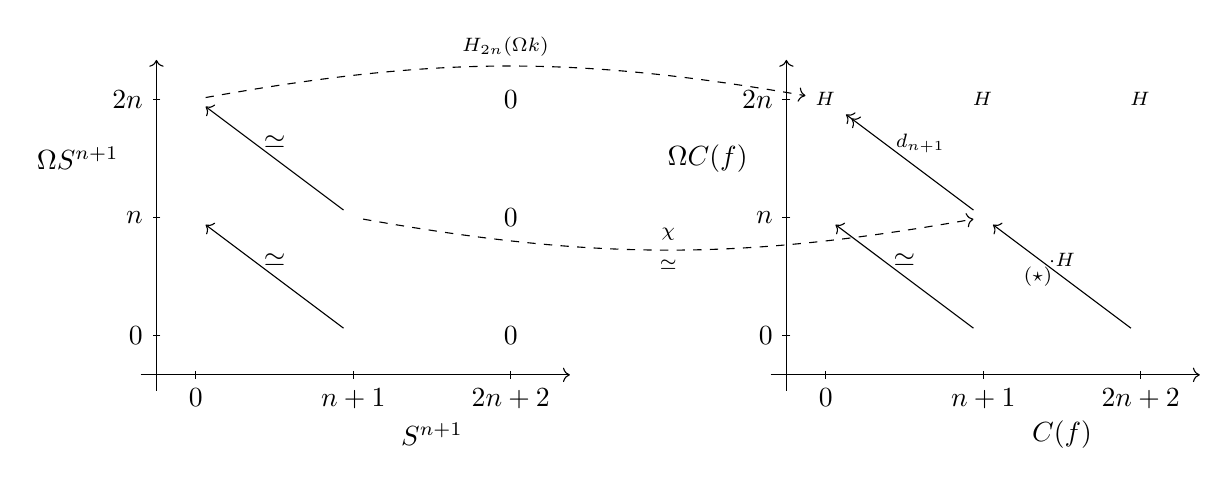
\begin{tikzpicture}
    %Axes
	\path (-1,2.75) node {$\Omega S^{n+1}$};
	\path (+3.5,-.76) node {$S^{n+1}$};
    \draw[->] (-0.2,0) -- (5.25,0);
    \draw[->] (0,-0.2) -- (0,4);
    %Horizontal ticks
    \draw (.5,.05) -- (.5,-.05) node[below] {$0$};
    \draw (2.5,.05) -- (2.5,-.05) node[below] {$n+1$};
    \draw (4.5,.05) -- (4.5,-.05) node[below] {$2n+2$};
    %Vertical Ticks
    \draw (.05,.5) -- (-.05,.5) node[left] {$0$};
    \draw (.05,2) -- (-.05,2) node[left] {$n$};
    \draw (.05,3.5) -- (-.05,3.5) node[left] {$2n$};
    %Points
    \path (.5,.5) node (v00) {$\Z$};
    \path (2.5,.5) node (v10) {$\Z$};
    \path (4.5,.5) node (v20) {$0$};
    \path (.5,2) node (v01) {$\Z$};
    \path (2.5,2) node (v11) {$\Z$};
    \path (4.5,2) node (v21) {$0$};
    \path (.5,3.5) node (v02) {$\Z$};
    \path (2.5,3.5) node (v12) {$\Z$};
    \path (4.5,3.5) node (v22) {$0$};
    %Arrow
    \draw [->] (v10) edge node[above]{$\simeq$} (v01);
    \draw [->] (v11) edge node[above]{$\simeq$} (v02);

%	\draw[dashed,->] (5.5,2) -- (7,2);
%	\draw[dashed,->] (5.5,2+1.5) -- (7,2+1.5);
%	\draw[dashed,->] (5.5,2-+1.5) -- (7,2-1.5);



    %Axes
	\path (8-1,2.75) node {$\Omega C(f)$};
	\path (8+3.5,-.76) node {$C(f)$};
    \draw[->] (7.8,0) -- (13.25,0);
    \draw[->] (8,-0.2) -- (8,4);
    %Horizontal ticks
    \draw (8.5,.05) -- (8.5,-.05) node[below] {$0$};
    \draw (10.5,.05) -- (10.5,-.05) node[below] {$n+1$};
    \draw (12.5,.05) -- (12.5,-.05) node[below] {$2n+2$};
    %Vertical Ticks
    \draw (8.05,.5) -- (8+-.05,.5) node[left] {$0$};
    \draw (8+.05,2) -- (8+-.05,2) node[left] {$n$};
    \draw (8+.05,3.5) -- (8+-.05,3.5) node[left] {$2n$};
    %Points
    \path (8+.5,.5) node (w00) {$\Z$};
    \path (8+2.5,.5) node (w10) {$\Z$};
    \path (8+4.5,.5) node (w20) {$\Z$};
    \path (8+.5,2) node (w01) {$\Z$};
    \path (8+2.5,2) node (w11) {$\Z$};
    \path (8+4.5,2) node (w21) {$\Z$};
    \path (8+.5,3.5) node (w02) {$\Z_H$};
    \path (8+2.5,3.5) node (w12) {$\Z_H$};
    \path (8+4.5,3.5) node (w22) {$\Z_H$};
    %Arrow
    \draw [->] (w10) edge node[above]{$\simeq$} (w01);
%    \draw [->] (w20) edge node[above right]{$\cdot H$} (w11);
    \draw [->,font=\scriptsize] (w20)
		edge node[left]{$(\star)$} node[above]{$\cdot H$} (w11);
    \draw [->>,font=\scriptsize] (w11) edge node[above] {\ \ $\;d_{n+1}$} (w02);%node[above]{$\simeq$} (w02);
%    \draw [->] (w21) edge node[above]{$a$} (w12);

	\draw[dashed,->,font=\scriptsize]  (v02) edge [bend left=10] node[above] {$H_{2n}(\Omega k)$} (w02);
	\draw[dashed,->,font=\scriptsize]  (v11) edge [bend right=10] node[above] {$\chi$}node[below] {$\simeq$} (w11);
\end{tikzpicture}
\end{center}
As the right hand sequence converges to $H_*(\ptspace)$, we deduce that $H_{2n}(\Omega C(f))=\Z_H$, and the differential $d_{n+1}:E^{n+1}_{n+1,n}\to E^{n+1}_{0,2n}$ is the quotient map $\Z\to\Z_H$.

Now the map $k:S^{n+1}\to C(f)$ induces a morphism of spectral sequences,  from that of the fibration $\Loops S^{n+1} \to PS^{n+1} \to S^{n+1}$ to that of $\Loops C(f) \to PC(f) \to C(f)$, as drawn above. Moreover, the map of interest, $H_{2n}(\Omega k)$, is one of the two dashed arrows. The other dashed arrow, $\chi$, is an isomorphism, as it is induced by the isomorphisms $H_{n+1}(k):H_{n+1}(S^{n+1})\to H_{n+1}(C(f))$ and $H_{n}(\Omega k):H_n(\Omega S^{n+1})\to H_n(\Omega C(f))$. Consideration of the commuting square in the above diagram reveals that $H_{2n}(\Omega k)$ is surjective, and completes the proof.
\end{proof}

Maybe now we should show that there exists an element of Hopf invariant 1; all the results we have proven so far have been negative.  Let's see that an $H$-space structure $S^{n-1}$ yields an element of Hopf invariant one on $S^n$, then real, complex, quaternionic, and Cayley multiplication will provide elements of Hopf invariant one on $S^1$, $S^2$, $S^4$, and $S^8$.

We will construct such elements using the ``Hopf construction''; to understand this construction, it helps to look at it in extreme generality.  Remember from the beginning of the course that this takes a ``multiplication'' $\mu: X \times Y \to Z$ and yields a map $H\mu: X \ast Y \to \Suspend Z$.  The construction (see lecture \ref{IntroductionToVectorFieldsOnSpheres}) is by forming a morphism of pushout diagrams, pictured on the left and right faces of the following cube:
\def\therowsep{6.5em}
\def\thecolumnsep{12em}
\begin{ctikzcd}
X\times Y    \ar[rr,"\mu"]\ar[dd] && Z\ar[dd]\\
& CX\times Y \ar[rr,crossing over] &&[0.5em] CY\ar[dd] \\
X\times CY   \ar[rr]     && CZ \\
& X\ast Y    \ar[rr,"H(\mu)"]\ar[from=uu,crossing over]     && \Suspend Z
\drar[from=1-1, to=2-2]\drar[from=1-1, to=2-2,yshift=-\therowsep-0.2em, xshift=0.2em]
\drar[from=1-1, to=2-2,xshift=\thecolumnsep+0.1em,yshift=0.2em]\drar[from=1-1, to=2-2,xshift=\thecolumnsep,yshift=-\therowsep]
\end{ctikzcd}
To explain this pictorially, we represent $X$, $Y$ and $Z$ each as a single point, so that $X\ast Y$ is represented as an ``L'' shape:
\begin{center}
\begin{tikzpicture}
\path (1.25-6,0) node[below,font=\scriptsize] {$C_+X$};
\path (-6,0) node[below left,font=\scriptsize] {$X$};
\HopfDiagram{}{}{}{-6}{0}{BottomBar}
\path (-3,.75) node[left,font=\scriptsize] {$C_-Y$};
\path (-3,0) node[below left,font=\scriptsize] {$Y$};
\HopfDiagram{}{}{}{-3}{0}{LeftBar}
\HopfDiagram{}{}{}{0}{0}{}
\path (0,.75) node[left,font=\scriptsize] {$X\times C_-Y$};
\path (1.25,0) node[below,font=\scriptsize] {$C_+X\times Y$};
\path (0,0) node[below left,font=\scriptsize] {$X\times Y$};
\path (1.,.6) node {$X\ast Y$};
\end{tikzpicture}
\end{center}
Moreover, we represent $\Sigma Z$ as another $L$ shape, drawn a little larger (below, to the left). The map $H(\mu)$ can then be represented pictorially as in the center below. Finally, we observe that the cone on $X\ast Y$ is in fact simply $C_+X\times C_-Y$, as drawn on the right below.
\begin{center}
\begin{tikzpicture}
\HopfDiagram{}{}{WhiteBeard}{-3}{0}{nojoin}
\path (0-3.5,.75) node[left,font=\scriptsize] {$C_-Z$};
\path (1.25-3.5,-.5) node[below,font=\scriptsize] {$C_+Z$};
\path (0-3.5,-.5) node[left,font=\scriptsize] {$Z$\ };
\path (-2-.5,.3) node {$\Sigma Z$};

\HopfDiagram{}{}{BlackBeard}{0}{0}{}
\path (1,0) node[right,font=\scriptsize] {$X\ast Y$};
\path (1,-.5) node[right,font=\scriptsize] {$\Sigma Z$};


\HopfDiagram{}{}{}{3}{0}{cone}
%\path (4,.75) node[right,font=\scriptsize] {$C(X\ast Y)$};
%\path (4,.25) node[right,font=\scriptsize] {$C_+X\times C_-Y$};
\path (5.,.5) node[above,font=\scriptsize] {$C(X\ast Y)$}
node[below,font=\scriptsize] {{$C_+X\times C_-Y$}}
node[font=\scriptsize] {\rotatebox{90}{$=$}};
\end{tikzpicture}
\end{center}
For brevity, write $j$ for $H(\mu)$. Now we will be interested in the Hopf invariant of $j$, when $X=Y=Z=S^{n-1}$. In particular, we should consider the cofiber $C(j)$. We already understand $C(X\ast Y)$, and can represent this cofiber pictorially (below, left), where the red arrows indicate gluing. Moreover, since the composite $X \ast Y \to \Suspend Z \to C(j)$ is null-homotopic, it extends to a  map $k:C(X\ast Y)\to C(j)$
In fact, we obtain a map $k$ for every nullhomotopy of this composite, and the obvious choice of nullhomotopy gives rise to the obvious map $k$.
In fact, $k$ is a relative homeomorphism $(C(X\ast Y),X\ast Y)\to (C(j),Z)$. It is drawn below, on the right, where the subspaces that form the data of a pair of spaces are drawn in green:
\begin{center}
\begin{tikzpicture}
\HopfDiagram{}{}{ArrowBeard}{-3}{0}{cone}
\HopfDiagram{on}{on}{}{1.75}{0}{cone}
\HopfDiagram{on}{on}{ArrowBeard}{5}{0}{cone}
\path [->,font=\scriptsize] (3,0.5) edge node[above]{$k$} (4.25,0.5);
\end{tikzpicture}
\end{center}
%
%
%;
%That is, we have a commutative diagram:
%\[\xymatrix{
%X \ast Y  \ar[d]\ar[r]^j & \Suspend Z\ar[d] \\
%C(X \ast Y)  \ar[r]^{k} \ar[d]& C(j)\ar[d]\\
%C(X\ast Y)/(X\ast Y)\ar[r]^{\ \ \ \ \ \cong}&C(j)/\Sigma Z
%}\]
Now we have the following commuting diagram of relative diagonal maps of pairs of spaces.\footnote{Recall that for any pair $(W,A\cup B)$, there is a relative diagonal map $(W,A\cup B)\to (W,A)\times (W,B)\eqdef(W\times W,A\times W\cup W\times B)$.} Here, we still draw the subspace $A$ in a pair $(W,A)$ in green, and still indicate gluing by drawing red arrows.
\begin{center}
\begin{tikzpicture}
\HopfDiagram{}{on}{}{1}{0}{cone} %bottom left
\HopfDiagram{on}{}{}{2.5}{0}{cone}
\path (2.25,-.75)
node[above] {$(C_+X\times C_- Y,C_+X\times Y)$}
node {$\times$}
node[below] {$(C_+X\times C_- Y,X\times C_-Y)$};
\path (7.25,-1) node {$(C(j),C_+Z)\times(C(j),C_-Z)$};
\path (12.75,-1) node {$C(j)\times C(j)$};

\path (2.25,4.35) node {$(C_+X\times C_- Y,X\ast Y)$};
\path (7.25,4.35) node {$(C(j),\Sigma Z)$};
\path (12.75,4.35) node {$C(j)$};

\HopfDiagram{}{on}{ArrowBeard}{6}{0}{cone}
\HopfDiagram{on}{}{ArrowBeard}{8}{0}{cone}
\HopfDiagram{}{}{ArrowBeard}{11.5}{0}{cone}
\HopfDiagram{}{}{ArrowBeard}{13.5}{0}{cone}

\HopfDiagram{on}{on}{}{1.75}{3}{cone}
\HopfDiagram{on}{on}{ArrowBeard}{7}{3}{cone}
\HopfDiagram{}{}{ArrowBeard}{12.5}{3}{cone}

\path[->] (3.75,.5) edge (5.25,.5);
\path[->] (10.75,.5) edge (9.25,.5);
\path[->] (3,3.5) edge  node[above] {$k$}(6.25,3.5);
\path[->] (11.75,3.5) edge (8.25,3.5);
\path[->] (2.25,2.75) edge (2.25,1.25);
\path[->] (7.25,2.25) edge (7.25,1.25);
\path[->] (7.25+5.5,2.25) edge (7.25+5.5,1.25);

\path (2.25,.5) node {$\times$};
\path (7.25,.5) node {$\times$};
\path (12.75,.5) node {$\times$};
\end{tikzpicture}
\end{center}
We are particularly interested in the case where $X=Y=Z=S^{n-1}$. In this case, restricting $\mu$ to $S^{n-1}\times\{x_0\}$ gives a self map of $S^{n-1}$, whose degree we denote $a$. Similarly, we denote by $b$ the degree of the restriction to $\{x_0\} \times S^{n-1}$.
%\[\xymatrix{
%S^{n-1} \times \{x_0\}\ar[d]
%\ar[rd]^(.6){\ \ a=\deg\left(\mu|_{S^{n-1}\times\{x_0\}}\right)} \\
%S^{n-1}\times S^{n-1}\ar[r]^{\qquad\mu}&S^{n-1}
%&\ar@{~>}[r]&&S^{2n-1}\ar[r]^j& S^n\\
%\{x_0\} \times S^{n-1}\ar[u]
%\ar[ru]_(.6){\ \ b=\deg\left(\mu|_{\{x_0\} \times S^{n-1}}\right)} \\
%}\]
The claim is:
\begin{lem}
The Hopf invariant of $H(\mu):S^{2n-1}\to S^n$ is $\pm ab$.
\end{lem}

\begin{proof}
We use the above diagram of relative diagonal maps. Then the cofiber $C(j)$ of $j=H(\mu):S^{2n-1}\to S^n$ has only an $n$-cell and a $2n$-cell, so we can write $H^n(C(j))=\Z\langle x\rangle$ and $H^{2n}(C(j))=\Z\langle y\rangle$.

Now the inclusion of $C(j)$  in the pair $(C(j),C_+Z)$ is an isomorphism on $H^n$, and we will write $x\in H^n(C(j),C_+Z)$ for the element mapping to $x\in H^n(C(j))$. We'll do the same for $(C(j),C_-Z)$. Consider the element $x\otimes x\in H^{2n}((C(j),C_+Z)\times(C(j),C_-Z))$, in the context of the above diagram. We have:
\begin{ctikzcd}
ab\,x^{\sprod 2} & \lar[mapsto,"k^*"'] Hy \rar[mapsto,"2."] &  Hy\\
b\,x\otimes a\,x \uar[mapsto,"4."] & \lar[mapsto,"3."'] x\otimes x \rar[mapsto] & x\otimes x\uar[mapsto,"1."]
\end{ctikzcd}
with the following explanations:
\begin{enumerate}
\item This diagonal \emph{defines} the cup product on $C(j)$, so $x\otimes x\mapsto x\smile x=Hy$.
\item The inclusion $C(j)\hookrightarrow (C(j), S^n)$ is an isomorphism on $H^{2n}$.
%\item $k^*$ is an isomorphism on $H^*$ because $k$ is a relative homeomorphism.
\item We can do this one factor at a time. On the left factor, we must consider the effect of the inclusion $i:(C_+X\times C_-Y,C_+X\times Y)\to (C(j),C_+Z)$ on $H^n(\text{---,---})$. We have a diagram, in which the vertical arrows are inclusions inducing isomorphisms on $H^n(\text{---,---})$ (when $X=Y=Z=S^{n-1}$):
\begin{center}
\begin{tikzpicture}
\path (1.5,.5) node[left] {$(x_0\times C_-Y,x_0\times Y)$};
\path (6.75,.5) node[right] {$(C_-Z,Z)$};
\path (1.5,3.5) node[left] {$(C_+X\times C_- Y,C_+X\times Y)$};
\path (6.75+1.5,3.5) node[right] {$(C(j),C_+ Z)$};

\HopfDiagram{}{on}{}{1.75}{3}{cone}
\HopfDiagram{}{on}{ArrowBeard}{7}{3}{cone}
\HopfDiagram{}{on}{}{1.75}{0}{LeftBar}
\HopfDiagram{}{on}{WhiteBeard}{7}{0}{LeftBar}

\path[->,font=\scriptsize] (2,.5) edge node[above] {map of cones induced by $\mu|_{x_0\times Y}$}
node[below] {degree $b$ on $H^n(\text{---,---})$} (6.25,.5);
\path[->,font=\scriptsize] (3,3.5) edge node[above]{$i$} (6.25,3.5);
\path[->]  (1.75,1.25)edge (1.75,2.75);
\path[->] (6.5,1.25) edge (6.5,2.25);
\end{tikzpicture}
\end{center}
Note that we use the following commuting diagram to understand that the lower map has degree $b$:
\begin{ctikzcd}
H^n(x_0 \times C_-Y, x_0 \times Y) \dar["\cong","\partial"'] & \lar H^n(C_-Z, Z)\\
H^{n-1}(x_0\times Y) & \lar["(\mu|_{x_0\times Y})^*"',"\cdot b"] H^{n-1} (Z)\uar["\cong","\partial"']
\end{ctikzcd}
In particular, $i^*(x)$ is $b$ times a generator (and we call this generator $x$ as well).
\item This relative diagonal \emph{defines} the smash product map.
\end{enumerate}
Thus, $k^*(Hy)=ab\,x^{\sprod2}$, and as $k$ is a relative homeomorphism, this shows that $H=\pm ab$.
\end{proof}
\begin{cor}
There is a map of Hopf invariant one in $\pi_{2n-1}(S^n)$ for $n=1,2,4,8$.
\end{cor}
\begin{proof}
Apply the previous lemma to the Hopf construction $j=H(\mu)$ where $\mu:S^{n-1}\times S^{n-1}\to S^{n-1}$ is the H-space multiplication on $S^{n-1}$ given by viewing $S^{n-1}$ as the unit sphere in $\R$, $\C$, $\H$, or $\O$.
\end{proof}
% >>>
\fi
\BoxedNote{
\Bullet Under $\Sigma\Omega\Sigma S^n=\bigvee_{\!k\geq0}\Sigma S^{kn}$, we have a map $h_2:\Omega S^{n+1}\to\Omega S^{2n+1}$. Moreover, $H^{2n}(h_2)$ is an isomorphism. We can calculate all of $H^*(h_2)$ as we know the algebra structure on $\Omega S^k$.

\Bullet If $n$ is odd, or if $n$ is even and we localise at $(2)$, then a SSS argument shows that $F(h_2)$ has the same cohomology as $S^n$. Now the counit $\alpha:S^n\to \Omega S^{n+1}$ is an isomorphism on $H^n$, and $h_2\alpha$ is null,  so $\alpha$ can be taken to be the fiber.

\Bullet The fiber sequence $S^n\to\Omega S^{n+1}\to\Omega S^{2n+1}$ has a LES of homotopy, the EHP sequence. The tail end exactly proves the Freudenthal suspension theorem.

\Bullet A map $h:\pi_{2n+1}(S^{n+1})\to\pi_{2n+1}(S^{2n+1})\cong\Z$ appears. We prove that it is precisely the Hopf invariant.

\Bullet We examine more closely the Hopf construction, taking $\mu:X\times Y\to Z$ and returning $j=H(\mu):X\ast Y\to\Sigma Z$. If $X=Y=Z=S^{n-1}$, we prove that $j$ has Hopf invariant $ab$, where $a$ and $b$ are the degrees of the restrictions to each factor. This constructs a map of Hopf invariant one on $S^n$ for $n=1,2,4,8$.
}
\section{Whitehead products and the EHP spectral sequence} % <<<
\label{WhiteheadProductsAndTheEHPSS}
\ifx\OutputWhiteheadProductsAndTheEHPSS\undefined\else
OK, so now we'll go back to the EHP sequence, and conclude this look at the map $h$ by seeing what we get from the existence of elements of Hopf invariant 1.  Last time we constructed maps $\tau: S^{2n+1} \to S^{n+1}$ of Hopf invariant one (for $n=0,1,3,7$)\footnote{These maps are often denoted $\eta$, $\nu$ and $\sigma$ respectively.}, by applying the Hopf construction to H-space multiplications $\mu:S^n \times S^n \to S^n$.  We'll consider this map when $n=1,3,7$. To see this phenomenon in the EHP sequence, we view $\tau$ as an element of $\pi_{2n}(\Omega S^{n+1})$, examining the $\pi_{2n}$ level of the long exact sequence of the fibration $S^{n} \to \Loops S^{n+1} \stackrel{h}{\to} \Loops S^{2n+1}$.  We can fit $\tau$ into this picture:
\begin{ctikzcd}
S^n\rar & \Omega S^{n+1} \rar[wavy,"h"] & \Omega S^{2n+1}\\
\Omega S^{2n+1} \urar[wavy,"\Omega \tau"] & S^{2n} \lar["\alpha"']\uar["\overline\tau"']\urar[dashed,"q"']
\end{ctikzcd}
We have decorated this diagram for readability only. The dashed map $q$ is defined to be the composite $h\overline\tau$. The wavy maps are highlighted, as their composite is a self map of $\Omega S^{2n+1}$ which we would like to show is a homotopy equivalence. The diagram commutes, as the left triangle simply expresses that $\overline\tau$ is adjoint to $\tau$.

Now because $\tau$ has Hopf invariant one, and $h$ detects the Hopf invariant, $q$ must be homotopic to $\pm\alpha$ (where $\alpha$ is the adjoint of $\textup{Id}_{\Sigma S^{2n}}$). Now $\pi_{2n}(\alpha)$ is an isomorphism, so by the Hurewicz theorem, so is $H_{2n}(\alpha)$, and by universal coefficients, so is $H^{2n}(\alpha)$. In particular, the wavy composite induces an automorphism $H^{2n}(\Omega S^{2n+1})$. As $H^*(\Omega S^{2n+1})$ is a divided polynomial algebra, it follows that the wavy composite is a cohomology isomorphism, and (by the Whitehead theorem) a homotopy self-equivalence
%(WTF\footnote{By the Whitehead theorem, even when $n=0$, as the spaces involved are \emph{simple} --- $\pi_1$ acts trivially on $\pi_n$ for all $n$.})
of $\Omega S^{2n+1}$.

This is amazing: it means that $\Loops S^{n+1}$ splits, and so the long exact sequence for this fibration splits into split short exact sequences:
\begin{ctikzcd}
0 \rar & \pi_j(S^n) \rar["e"] & \pi_{j}(\Loops S^{n+1})\rar[yshift=0.3em,"h"] & \pi_j(\Loops S^{2n+1}) \lar[wavy,yshift=-0.3em,"(\Omega\tau)_*"] \rar & 0
\end{ctikzcd}
Now addition on $\pi_j(\Omega S^{n+1})$ is induced\footnote{Note that from this fact, (i.e.\ that if $X$ is a connected H-space then addition on $\pi_*(X)$ is induced by the multiplication), it follows that the fundamental group of an H-space is abelian.} by the loop multiplication $\mu$ on $\Omega S^{n+1}$, so that the composite
\begin{ctikzcd}
S^n\times \Loops S^{2n+1} \rar["e\times \Loops \tau"]\ar[rr,bend right=10,yshift=-0.3em,"C"'] & \Loops S^{n+1}\times \Loops S^{n+1}\rar["\mu"] & \Loops S^{n+1}
\end{ctikzcd}
induces the following composite on homotopy groups, which is an isomorphism:
\begin{ctikzcd}
\pi_j(S^n\times \Loops S^{2n+1})\rar[equal] &[-0.5em] \pi_j(S^n)\times\pi_j(\Omega S^{2n+1}) \rar["e\times (\Omega\tau)_*"{yshift=0.1em}]
    &[1em] \pi_j(\Omega S^{n+1})\times \pi_j(\Omega S^{n+1})\rar["\text{add}"{yshift=0.1em}] & \pi_j(\Omega S^{n+1})
\end{ctikzcd}

Thus $C$ is a homotopy equivalence,\footnote{By the Whitehead theorem. Note that this agument applies when $n=1$, as both spaces involved are \emph{simple} spaces. A simple space is one in which the action of $\pi_1$ on $\pi_n$ is trivial for all $n$. Note that all H-spaces are simple, as all Whitehead products are zero in an H-space. See below.} and this \emph{never} happens for other $n$, as it is equivalent to the existence of an element of Hopf invariant one. To re-emphasise, on homotopy groups we have isomorphisms:
\begin{ctikzcd}[row sep=tiny]
\pi_j( S^n) \times \pi_{j+1} (S^{2n+1} ) \rar["\cong"] & \pi_{j+1} (S^{n+1}) \\
(\alpha, \beta) \rar[mapsto] & e \alpha + \tau_*(\beta)
\end{ctikzcd}
OK, now let's talk about the ``P'' part of the EHP sequence; ``P'' stands for product, I guess, so first let's take a step back and talk about Whitehead products.  I'm not going to prove everything; for more information, refer to George Whitehead's novel~\cite{Whitehead}.

The Whitehead product is a map $\pi_p (X) \times \pi_q (X) \to \pi_{p+q-1} (X)$, which is easiest to describe in terms of its universal example, a map $W: S^{p+q-1} \to S^p \wsum S^q$. With $W$ understood, then for $\alpha \in \pi_p (X)$, $\beta \in \pi_q (X)$, we define the Whitehead product $[\alpha, \beta] \in \pi_{p+q-1} (X)$ to be the composite:
\begin{ctikzcd}
S^{p+q-1} \rar["W"] & S^p \wsum S^q \rar["\alpha \wsum \beta"] & X \wsum X \rar["\Phi"] & X.
\end{ctikzcd}

The map $W$ is constructed as follows: $S^p \times S^q$ has three non-zero cells; the first two compromise the axes $S^p \wsum S^q$, and the third is a $(p+q)$-cell whose attaching map is the map $W: S^{p+q-1} \to S^p \wsum S^q$.
\ConfusedBox{\textbf{I've removed a bunch of pictures that aren't looking too good. Maybe some of them will get replaced a little later.}

\textbf{I don't really see the correctness/usefulness of the following statement:} So the top dimensional cell is the mapping cone of $W$.}
%\begin{wrapfigure}{r}{0.3\textwidth}
%\centering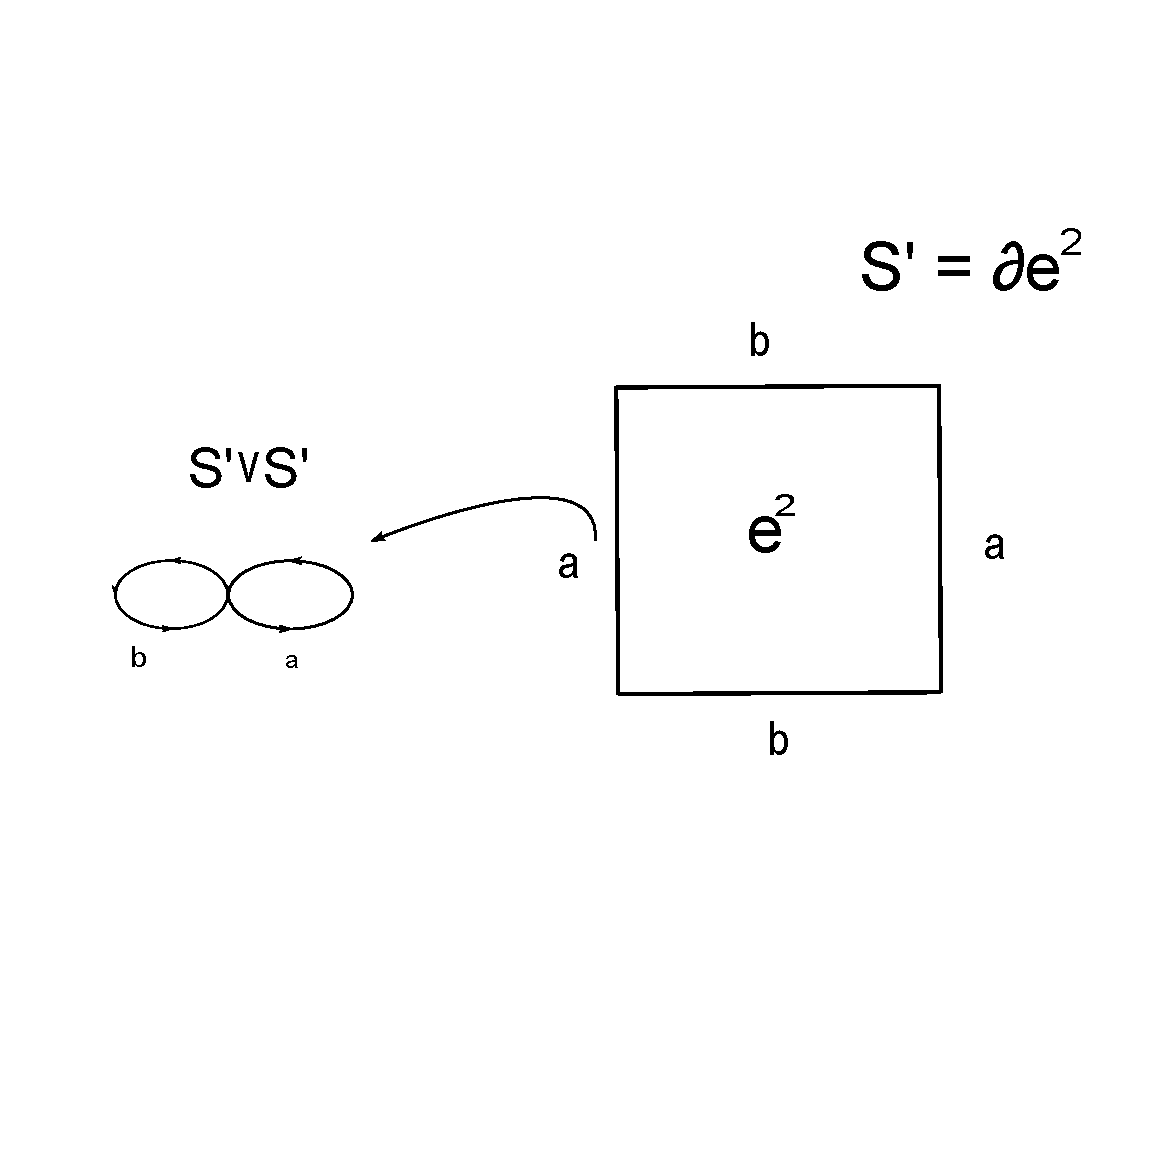
\includegraphics[width=0.3\textwidth]{figures/22.pdf}
%\caption{\small The example $S^1 \times S^1$.}
%\end{wrapfigure}
%\begin{figure}[h!]
%\centering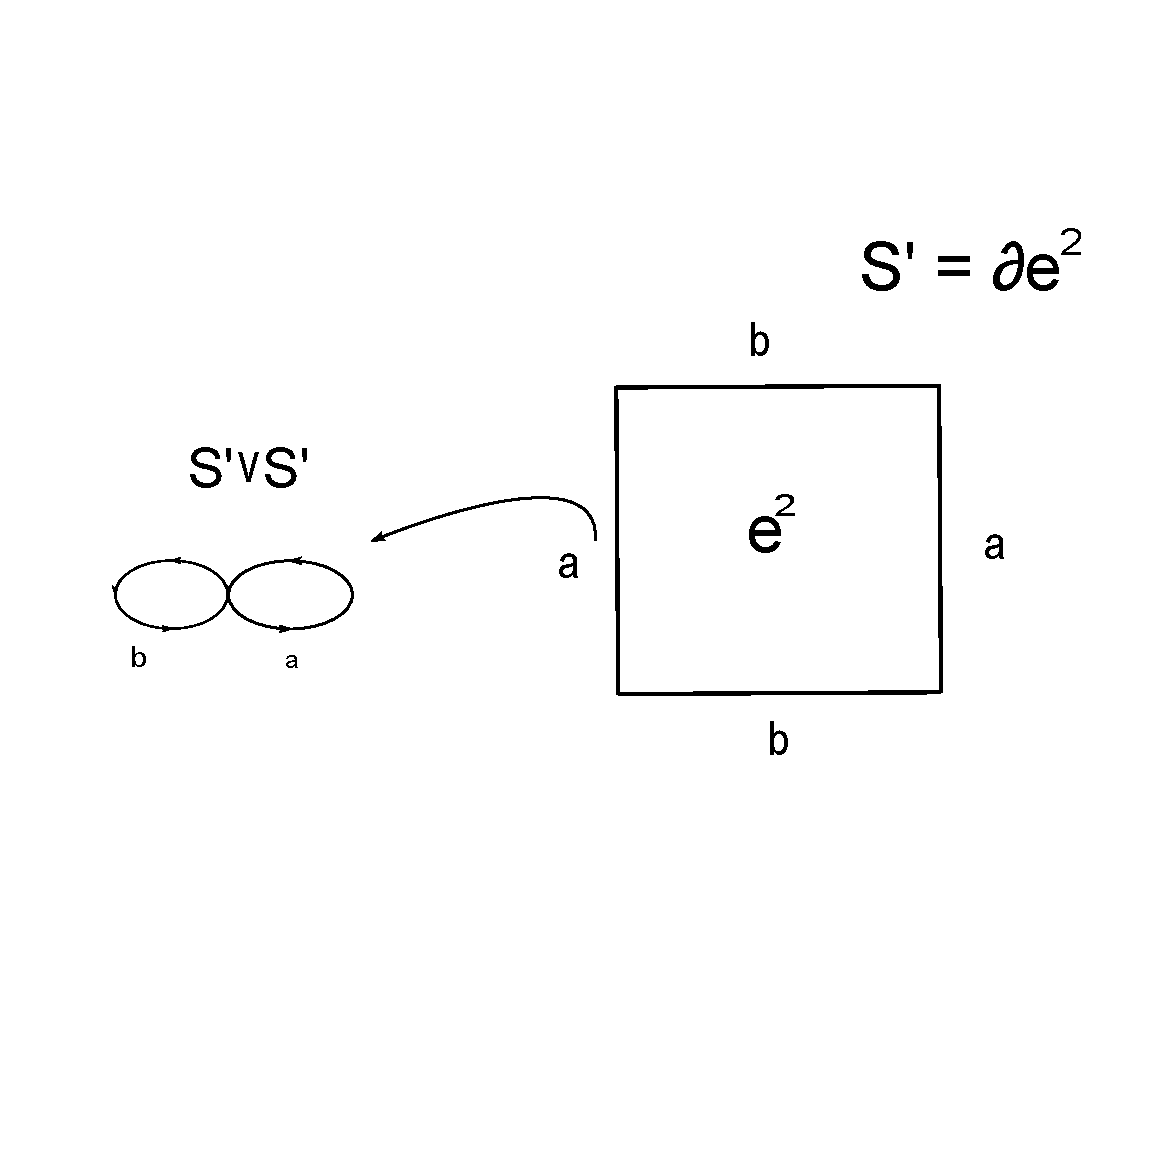
\includegraphics[width=0.3\textwidth]{figures/22.pdf}
%\caption{\small The example $S^1 \times S^1$.}
%\end{figure}
Another way to think about $W$ is as follows. $S^{p}\times S^{q}$ is a quotient of $e^p\times e^q$, under the product of the quotient maps $\pi:e^p\to S^p$ and $\pi':e^q\to S^q$ given by collapsing boundaries. In fact, this quotient map is part of a pushout diagram (drawn on the left):
\begin{cjointikzcd}[intertext,row sep=small]
\diagram
    e^p\times e^q \rar["\pi\times \pi'"] & S^p\times S^q\\
    \edgellap{S^{p+q-1}=}\partial(e^p\times e^q) \uar[hook] \rar["W"] & S^p\vee S^q \uar[hook]
%
\diagram \intertext{where}
%
\diagram
    e^p\rar["\pi"] & S^p \vee S^q & \lar["\pi'"] e^q\\
    e^p\times S^{q-1} \uar["\textup{pr}_1"] \rar[hook] & \partial(e^p\times e^q) \uar["W"] & \lar[hook'] S^{p-1} \uar["\textup{pr}_2"']
\end{cjointikzcd}
\ConfusedBox{I could probably put the diagram from my notes here.}
Facts about the Whitehead product: once again, for real proofs, see Whitehead's book.
\begin{enumerate}
\item In the case $p = q = 1$ it is a map $\pi_1 (X) \times \pi_1 (X) \to \pi_1 (X)$, given by $[\alpha, \beta] = \alpha \beta \alpha^{-1} \beta^{-1}$, as can be seen by considering the attaching map of the top cell of the torus. This justifies the bracket notation.  In the case $p = 1$ and $q \ge 1$, this product gives the natural action of $\pi_1 (X)$ on $\pi_q (X)$.
\item Skew commutativity: $[\beta, \alpha] = (-1)^{|\alpha||\beta|}[\alpha, \beta]$.
\item The Jacobi identity: for $\alpha \in \pi_p (X)$, $\beta \in \pi_q (X)$, $\gamma \in \pi_r (X)$:
\[
(-1)^{(r-1)p}[\alpha, [\beta, \gamma]] + (-1)^{(p-1)q}[\gamma, [\alpha, \beta]] + (-1)^{(q-1)r}[\beta, [\gamma, \alpha]] = 0
.\]
\item Interaction with the Hurewicz map.  One way to straighten out the degree shift is to write all the homotopy groups in terms of $\Loops X$; then the Whitehead product is a map $\pi_p (\Loops X) \times \pi_q (\Loops X) \to \pi_{p+q} (\Loops X)$.  On the other hand there is the Hurewicz map $h: \pi_* (\Loops X) \to H_* (\Loops X)$ (and $H_*(\Loops X)$ is a noncommutative algebra with Pontryagin product). Then $h([\alpha, \beta]) = h(\alpha)h(\beta) - h(\beta)h(\alpha)$, i.e., $h$ is a map of Lie algebras.
\item The suspension $\Suspend [\alpha, \beta] = 0$.  We know this fact, that $X \wsum Y \to X \times Y$ splits after one suspension, so that $\Suspend W$ is nullhomotopic.
\item If $X$ is an H-space, then $[\alpha, \beta] = 0$.  This follows from the commutative diagram:
\begin{ctikzcd}
S^{p+q-1} \drar \rar["W"] & S^p \wsum S^q \dar\rar["\alpha \wsum \beta"] & X \wsum X \dar\rar["\Phi"] & X \\
& S^p \times S^q \rar["\alpha \times \beta"] & X \times X\urar["\mu"']
\end{ctikzcd}
\end{enumerate}

Now consider the Whitehead product in the case $p = q = n$; here the most interesting case is the ``Whitehead square'' $[\alpha, \alpha]$.  It can be computed in terms of its universal example $[\iota_n, \iota_n] = w_n$, where $\iota_n$ is the fundamental class in $\pi_n (S^n)$. That is, for $\alpha\in\pi_p(X)$, $[\alpha,\alpha]\in\pi_{2p-1}(X)$ is the composite $\alpha \circ w_n$:
\begin{ctikzcd}[column sep=0pt]
S^{2p-1} \ar[rr,"w_n"]\ar[dr,"W"'] && S^p \ar[rr,"\alpha"] &[0.5em]& X\\
 & S^p\vee S^p \ar[ur,"\Phi"'] \ar[rr,"\alpha\vee \alpha"'{yshift=-0.1em}] && X\vee X \urar["\Phi"']
\end{ctikzcd}
Now before, we saw that $W$ was part of a pushout square, drawn on the left below. We also have it that $\Phi$ is part of an adjoining pushout square, drawn at the right:
\begin{ctikzcd}
e^p\times e^p\rar["\pi\times\pi'"]&S^p\times S^p\rar&J_2(S^p)\\
\edgellap{S^{2p-1}=}\partial(e^p\times e^p)\uar[hook]\rar["W"]&S^p\vee S^p\uar[hook]\rar["\Phi"] &S^p\ar[u]
\end{ctikzcd}
Now the outer square is a pushout diagram, and the inclusion of $S^{2p-1}$ in the contractible space $e^p\times e^p$ is a cofibration, so that $J_2(S^n)$ is the mapping cone $C(w_n)$.
%But this all means that the mapping cone $C(W_n) = J_2 S^n$, the second filtration of the free monoid on $S^n$, $JS^N$, from the James construction.

Now $w_n \in \pi_{2n-1} (S^n)$ so we should compute its Hopf invariant, and the inclusion $J_2(S^n)\hookrightarrow J(S^n)\simeq\Omega S^{n+1}$  induces an isomorphism on cohomology algebras up to degree $2n$.\footnote{Recall that after one suspension, $J_2(S^n)$ splits as $\Sigma J_2(S^n)=\bigvee_{\!k\leq2}S^{nk+1}$, compatibly with the splitting $\Sigma J_2(S^n)=\bigvee_{\!k}S^{nk+1}$. In particular, the inclusion $J_2(S^n)\to J(S^n)$ is an isomorphism on homology and cohomology up to degee $2n$.\label{Fottnoteofold}} Moreover, % and we already have a good start since we know that $C W_n = J_2 S^n$.  Now from the James construction we know that $J_2 S^n \into \Loops S^{n+1}$, and moreover
\[
H^* (\Loops S^{n+1} )\cong \begin{cases} \Gamma[x_1] & \hbox{$n$ even} \\ E[x_1] \otimes \Gamma[x_2] & \hbox{$n$ odd} \end{cases}
\raisebox{-.0cm}{\ \ \  which shows that\ \ \ }
H (w_n)= \begin{cases}2 & \hbox{$n$ even} \\ 0 & \hbox{$n$ odd}\end{cases}
\]
Well, this is pretty nice, in fact it's pretty amazing: what we've done is look at
\[
\pi_{2n-1} (S^n) \stackrel{h}{\to} \pi_{2n-1}(S^{2n-1}) = \Z
\]
and show that the image contains $2\Z$ is $n$ is even. Thus there is a short exact sequence
\[0\to \ker (h)\to\pi_{2n-1}(S^n)\to\left(\im(h)\cong\Z\right)\to0.\]
As $\Z$ is free, this sequence splits, and $\pi_{2n-1}(S^n)\simeq\ker(h)\oplus\Z$. This, and $\pi_n (S^n) = \Z$ are in fact the only free abelian summands in higher homotopy groups!  Now if you're away from $2$, $2$ is as good as one; in other words a corollary of the above and our calculation of $H^* (\Loops S^{n+1})$ is:
\ConfusedBox{\textbf{Don't we also need to be away from all the other primes, so that the EHP sequence is a fiber sequence? I.e. Doesn't this need to be done rationally?} Wait, maybe not! `the above' may simply refer to what's a couple of lines above this box.}
\begin{cor}
For $n$ even, away from $2$, $\Loops S^n \simeq S^{n-1} \times \Loops S^{2n-1}$, i.e.:
\[\pi_{*+1} (S^n) \otimes \Z[\nicefrac{1}{2}] \cong (\pi_* (S^{n-1}) \oplus \pi_{*+1} (S^{2n-1})) \otimes \Z[\nicefrac{1}{2}].\]
\end{cor}
Now remember the $h$ map appeared in the long exact sequence
\begin{ctikzcd}
\pi_{k+n} (S^n) \rar["e"] & \pi_{k+n+1} (S^{n+1})\rar["h"]&\pi_{k+n+1} (S^{2n+1}) \\
\end{ctikzcd}
as the obstruction to desuspending a class in $\pi_{k+n+1} (S^{n+1})$, so that:
\begin{cor}
For $n$ odd, $w_{n-1} \in \pi_{2n-3} (S^{n-1})$ doesn't desuspend, and for $n$ even it desuspends at least once.
\end{cor}
Now $w_{n-1}$ might desuspend more times; you might ask where  it was ``born'' in the sequence
%\[
%\cdots \stackrel{e}{\to} \pi_{k+n} S^n \stackrel{e}{\to} \pi_{k+n+1} S^{n+1} \stackrel{e}{\to} \pi_{k+n+2} S^{n+2} \stackrel{e}{\to} \cdots
%\]
\begin{ctikzcd}
\cdots \rar &\pi_{2n-6}(S^{n-4}) \rar["e"] & \pi_{2n-5}(S^{n-3}) \rar["e"] & \pi_{2n-4}(S^{n-2}) \rar["e"] &\pi_{2n-3}(S^{n-1})
\end{ctikzcd}
And here we see the (as yet) mysterious rebirth of the vector field problem:
\begin{thm}
$w_{n-1} \in \pi_{2n-3} (S^{n-1})$ desuspends to an element in $\pi_{2n-\rho(n)-2}(S^{n-\rho(n)})$ and no further. That is, $w_{n-1}$ desuspends exactly $\rho(n)-1$ times.\footnote{Recall that $\rho(n)$ was the number from the vector field problem (see lecture \ref{IntroductionToVectorFieldsOnSpheres}):
$
\begin{array}{c|cccccccc}
n & 1 & 2 & 4 & 8 & 16 & 32 & 64 & \cdots \\
\hline
\rho(n) & 1 & 2 & 4 & 8 & 9 & 10 & 12 & \cdots
\end{array}
$}
\end{thm}
Now in order to prove this theorem, we have to relate $w_n$ to the EHP sequence; here's one way:
\begin{thm} The Whitehead square factors as:
\begin{ctikzcd}
S^{2n-1}\drar["\pm w_n"']\rar["e^2"] & \Loops^2S^{2n+1}\dar["p"]\\
 & S^n
\end{ctikzcd}
In particular, under $p:\pi_k (S^{2n+1}) \to \pi_{k-2} (S^n)$ we have $e^2 \alpha\longmapsto \pm w_n \circ \alpha$ \textup{(}for any $\alpha\in\pi_{k-2}(S^{2n-1})$\textup{)}.  This is why the $p$ map is called the ``Whitehead product''.\footnote{However, the behavior of $p$ on a class which is not a double suspension is more erratic.}
\end{thm}
\begin{proof}
Starting with the undecorated arrows in the following diagram, we obtain the wavy arrow since $e\circ w_n$ is null, and the dotted arrow by exactness of
\begin{tikzcd}
\pi_{2n+1}(S^{2n+1})\rar["p"] & \pi_{2n-1}(S^n)\rar["e"]& \pi_{2n}(S^{n+1}):
\end{tikzcd}
%
\begin{ctikzcd}[row sep=2.4em]
S^{2n-1} \dar[dashed]\rar["w_n"] & S^n\dar[equal]\rar & C(w_n)\dar[wavy]\\
\Loops^2S^{2n+1} \rar["p"] & S^n \rar["e"] & \Loops S^{n+1}
\end{ctikzcd}
%
All we need to show is that the dashed map is $\pm e^2$. By the Hurewicz theorem, it is enough to show that it induces an epimorphism on $H_{2n-1}$. This follows from the diagram
\begin{ctikzcd}
\Htwee_{2n} (C (w_n)) \rar["(1)","\cong"'] & \Htwee_{2n} (\Loops S^{n+1}) \\
%
H_{2n}(S^n, w_n (S^{2n-1})) \rar \uar["\cong"']\dar["\cong","\partial"']
& H_{2n}(S^n, p(\Loops^2 S^{2n+1}) )\uar["\cong"',"(2)"]\dar["\cong","\partial"']\\
%
H_{2n-1} (S^{2n-1}) \rar[dashed] & H_{2n-1} (\Loops^2 S^{2n+1})
\end{ctikzcd}
if we verify that the maps (1) and (2) are isomorphisms.  We showed that (1) is an isomorphism in a previous footnote.$^\text{\ref{Fottnoteofold}}$
\todo{Remove this from the footnote.}
That (2) is an isomorphism follows from the following argument involving the spectral sequence of the fibration $\Loops^2 S^{2n+1} \to S^n \to \Loops S^{n+1}$. For ease of reading, write $F\to E\to B$ for the three terms of this fibration. Then the transgression $E^{2n}_{2n,0}\to E^{2n}_{0,2n-1}$ must be an isomorphism, however, there can be no other nonzero differentials in or out of $E_{2n,0}$ and $E_{0,2n-1}$. Now the following diagram defines the transgression:
\begin{ctikzcd}
H_{2n-1}(F)&\ar[l]H_{2n}(E,F)\ar[r,"(2)"]&H_{2n}(B,*)&%\ar[r]& &&%H^n(\Omega B)\ar@{=}[r]&H^{n+1}(\Sigma\Omega B)&\ar[l]
H_{2n}(B)\ar[l]
\end{ctikzcd}
If (2) were not an isomorphism, then the transgression could not be either.
\end{proof}
One consequence of this is
\begin{cor}
$\iota_{2n+1} \mapsto \pm w_n$ under $p:\pi_{2n+1}(S^{2n+1})\to\pi_{2n-1}(S^n)$.
\end{cor}
And so we get
\begin{thm}[G.\ Whitehead]
The kernel of \begin{tikzcd}\pi_{2n-1}(S^n)\rar["e"]&\pi_{2n}(S^{n+1})\end{tikzcd}\!\! is
%
%In the exact sequence
%$\xymatrix{\pi_{2n+1}(S^{2n+1})\ar[r]^{\ p}&\pi_{2n-1}(S^n)\ar[r]^e&\pi_{2n}(S^{n+1})}$\!,
\[
\ker(e) = \begin{cases} 0 & \hbox{when $n = 1, 3, 7$} \\ \Z_2 \langle w_n \rangle & \hbox{$n$ odd, $n\neq1,3,7$} \\ \Z \langle w_n \rangle & \hbox{$n$ even}. \end{cases}
\]
\end{thm}
\begin{proof}
We'll focus on the excerpt
\begin{tikzcd}
\pi_{2n+1}(S^{n+1})\rar["h"] & \pi_{2n+1}(S^{2n+1})\rar["p"] & \pi_{2n-1}(S^n)\rar["e"]&\pi_{2n}(S^{n+1})
\end{tikzcd}.
We can describe $\ker(e)=\im(p)$ as the subgroup generated by $\pm p(\imath_{2n+1})=w_n$.

When $n=1,3,7$, there is an element of Hopf invariant one in $\pi_{2n+1}(S^{n+1})$, so that $h$ is surjective, and $p=0$. In particular, $w_n=0$.

When $n\neq1,3,7$ is odd, there is an element of Hopf invariant two in $\pi_{2n+1}(S^{n+1})$, but no element of Hopf invariant one, so that $\im(h)$ has index two in $\pi_{2n+1}(S^{2n+1})$.

When $n$ is even, $w_n$ has hopf invariant two, and so has infinite order.
\end{proof}

Now we want to address the desuspension problem, and in order to do that we'll link up all the EHP sequences. Here they are:
\begin{ctikzcd}
S^n \rar["e"] & \Loops S^{n+1}\rar["h"] & \Loops S^{2n+1};
\end{ctikzcd}
apply $\Loops^n$ to get
\begin{ctikzcd}
\Loops^n S^n \rar["e"] & \Loops^{n+1} S^{n+1} \rar["h"] & \Loops^{n+1} S^{2n+1}.
\end{ctikzcd}
Now these link together:
\begin{ctikzcd}
\ptspace \rar["e"] & \Loops S^1 \dar["h"]\rar["e"] & \Loops^2 S^2 \dar["h"]\rar["e"] & \Loops^3 S^3 \dar["h"]\rar["e"] & \cdots \rar & \bigcup \Loops^n S^n = QS^0 \\
& \Loops S^1 & \Loops^2 S^3 & \Loops^3 S^5,
\end{ctikzcd}
Here, $e:\Omega^{n}S^{n}\to\Omega^{n+1} S^{n+1}$ can be viewed as the
$n$-fold looping of the inclusion of the straight loops $S^{n}\to\Omega S^{n+1}$. In particular, each $e$ realises the suspension homomorphism on homotopy. Moreover, $QS^0$ is given the quotient (a.k.a.\ direct limit) topology, and as such (as $S^k$ is compact):
\[\pi_k(QS^0)=[S^k,\varinjlim\Omega^n S^n]=\varinjlim[S^k,\Omega^n S^n]=\varinjlim\pi_{k+n}(S^n)=\Pi_k.\]
We also note that the map $\pi_k(\Omega^n S^n)\to\Pi_k$ induced by mapping $\Omega^n S^n\to QS^0$ is the stabilisation map.

In particular, this sequence has filtered the stable homotopy groups of spheres by unstable homotopy groups.  But each leg is a fibration, and the corners match, so if you apply homotopy something wonderful happens: you get a sequence of exact triangles whose ends match up (the maps $p$ have degree $-1$ on $\pi_*$).
\begin{ctikzcd}
\pi_*(\ptspace) \rar["e"] & \pi_*(\Loops S^1) \dar["h"]\rar["e"] & \pi_*(\Loops^2 S^2) \dar["h"]\rar["e"] & \pi_*(\Loops^3 S^3) \dar["h"]\rar["e"] & \cdots \rar & \Pi_* \\
& \pi_*(\Loops S^1)\ular["p"] & \pi_*(\Loops^2 S^3)\ular["p"] & \pi_*(\Loops^3 S^5)\ular["p"],
\end{ctikzcd}
This is an \emph{exact couple}, so you get a spectral sequence converging to $\pi_* (Q S^0)=\Pi_*$, whose $E_1$ page consists of the bottom line of the above diagram:
\[
E^1_{s, t} = \pi_{s+t}(\Loops^{s+1} S^{2s+1}) = \pi_{2s+1+t} (S^{2s+1})
\]
so the columns of the spectral sequence are homotopy groups of odd spheres.  So here it is:
\missingfigure{$E_1$ page of the EHPSS}
The differentials $d_r: E^r_{s, t} \to E^r_{s-r, t+r-1}$, of total degree $-1$, are like the differentials in the usual homology spectral sequence. They are `defined' by the `formula' $d_r=he^{-(r-1)}p$, that is:
\begin{ctikzcd}[row sep=large]
\pi_{s+t-1}(\Omega^{s-r+1}S^{s-r+1})\dar["h"]\rar["\text{r-1}","\text{desuspensions}"'] &[width("desuspensions")-\pgfmatrixcolumnsep] \pi_{s+t-1}(\Omega^s S^s)\\
\edgellap{E^1_{s-r,t+r-1}=}\pi_{s+t-1}(\Loops^{s-r+1}S^{2s-2r+1}) && \mathllap{E^1_{s,t}=}\pi_{s+t}(\Omega^{s+1}S^{2s+1})\ular["p"]
\end{ctikzcd}
Of course, this `definition' does not make sense on the groups $E^1_{s,t}$. Instead, it makes sense on the subquotients $E^r_{s,t}$ of the $E^1_{s,t}$. In fact, we may define, for $0\leq r\leq\infty$:\footnote{One should check that this definition gives $E^1_{s,t}=\pi_{s+t}(\Omega^{s+1}S^{2s+1})$, and that can be made to make sense when $r=\infty$. By convention, we regard $\Omega^n S^n$ to be the one point space when $n<0$.}
\begin{alignat*}{2}
Z_{st}^r\eqdef&\left\{x\in \pi_{s+t}(\Omega^{s+1}S^{2s+1})\ \middle|\ p(x)\in\im(e^{r})\right\}\\
=&\left\{x\ \middle|\ \text{$p(x)\in\pi_{s+t-1}(\Omega^s S^s)$ desuspends to an element of $\pi_{s+t-1}(\Omega^{s-r} S^{s-r})$}\right\}.\\
B_{st}^r\eqdef&\left.h(\ker(e^r))\right.\\
=&\left\{h(y)\ \middle|\ y\in \pi_{s+t}(\Omega^{s+1}S^{s+1}),\ e^r(y)=0\in \pi_{s+t}(\Omega^{s+r+1}S^{s+r+1})\right\}\\
=&\left\{\text{James-Hopf invariants $h(y)$ of classes $y$ vanishing after $r$ suspensions}\right\}.\\
E_{st}^{r+1}\eqdef&\left.Z_{st}^r/B_{st}^r.\right.
\end{alignat*}
Given this definition, and the above definition of the differentials $d_r$, it is an exercise in diagram chasing to check that we have given the data of a spectral sequence.

For each $s,t\geq0$, let $e_{st}:\pi_{s+t}(\Loops^{s+1} S^{s+1})\to \Pi_{s+t}$ be the stabilisation homomorphism. Then there is an increasing filtration on $\Pi_{s+t}$ defined by $F_{s}\Pi_{s+t}\eqdef\im(e_{st})$. Let $\Gr_{st}$ be the subquotient $F_{s}\Pi_{s+t}/F_{s-1}\Pi_{s+t}$:
%\[\Gr_{st}\eqdefF_{s}h_{s+t}(E)/F_{s-1}h_{s+t}(E).\]
%With this notation:
\[
\Gr_{st}\eqdef\frac{\im\bigl(\pi_{s+t}(\Omega^{s+1} S^{s+1})\rightarrow \Pi_{s+t}\bigr)}{\im\bigl(\pi_{s+t}(\Omega^s S^{s})\rightarrow \Pi_{s+t}\bigr)}.\text{\ \ \ Note also:\ \ }
Z_{st}^\infty=
h(\pi_{s+t}(\Omega^{s+1}S^{s+1}));\text{\ and\ }
B_{st}^\infty=h(\ker (e_{st})).
\]
The spectral sequence converges to $\Pi_{s+t}$, in that there are isomorphisms $E_{st}^\infty\to \Gr_{st}$ defined by:
\[[h(y)]\longmapsto [e_{st}(y)]\text{ for $y\in \pi_{s+t}(\Omega^{s+1}S^{s+1})$}\]
Now if $z\in F_s\Pi_{s+t}$, then there is some $\overline z\in \pi_{s+t}(\Omega^{s+1} S^{s+1})$ such that $e_{st}(\overline z)=z$. The inverse isomorphism $\Gr_{st}\to E_{st}^\infty$ is then given by:
\[[z]\longmapsto [h(\overline z)].\]
That is to say the following. Given an element $z\in\Pi_n$ in the stable $n$-stem, desuspend $z$ as far as possible to an element of $\overline z\in\pi_{n}(\Omega^{s+1}S^{s+1})$, then $h(\overline z)\in \pi_{n}(\Omega^{s+1}S^{2s+1})=:E^1_{s,n-s}$ is a permanent cycle detecting $z$. One could summarise by stating that $z$ is recorded by the James-Hopf invariant of a maximal desuspension.

Now an obvious question is this: if you think of a spectral sequence as a way of computing the $E^\infty$ term from the $E^1$ term, well, why isn't this game hopeless?  We have a spectral sequence converging to stable homotopy whose input is \emph{unstable} homotopy, which could very well be more difficult to compute.  But one really neat feature of this game is that in
\begin{ctikzcd}
\ptspace \rar["e"] & \Loops S^1 \dar["h"]\rar["e"] & \Loops^2 S^2 \dar["h"]\rar["e"] & \Loops^3 S^3 \dar["h"]\rar[equal] & \Loops^3 S^3\dar \rar[equal]& \cdots\\
& \Loops S^1 & \Loops^2 S^3 & \Loops^3 S^5 & 0
\end{ctikzcd}
we can just \emph{stop} the exact couple anywhere, and get an identical spectral sequence to the one we just saw except that we'll have zeroes in the columns beyond where we stop; otherwise, the picture is the same.  And the spectral sequence we get will converge to the homotopy of the sphere in the last column; in the case above, for example, $\pi_* (\Loops^3 S^3)$.  So actually we have a whole family of spectral sequences converging to the input of our original spectral sequence.

Well, that still doesn't sound very good, except that you can play all of these facts off each other and often you can get pretty far.  For example, let's look at $d_1$, the composite:
\begin{ctikzcd}
E^1_{s,t}= \pi_{s+1}(\Loops^{s+1}S^{2n+1}) \rar["p"] & \pi_{s+t-1}(\Loops^s S^s) \rar["h"] & \pi_{s+t-1}(\Omega^sS^{2s-1})=E^1_{s-1,t}
\end{ctikzcd}
On the bottom row (when $t=0$), $E^1_{s,t}$ and $E^1_{s-1,t}$ are both isomorphic to the integers. We only need to know what happens to the generator $\imath_{2s+1}$:
\[\imath_{2s+1}=e^2\imath_{2s-1}\overset{p}{\longmapsto}\pm \imath_{2s-1}\circ w_{s}=w_s\overset{h}{\longmapsto} \pm h(w_s)=\begin{cases}2\imath_{2s-1},&\text{$s$ even,}\\0,&\text{$s$ odd.}\end{cases}\]
Thus we have calculated the $d_1$ differential on the bottom row.
% we only need to know what happens to $\iota_{2s+1} \in \pi_s \Loops^{s+1} S^{2s+1} = \pi_{2s+1} S^{2s+1} = \Z \langle \iota_{2s+1} \rangle$.  But we already computed that considering that $\iota_{2s+1} \in \pi_{2s-1} \Loops^2 S^{2s+1}$, we get $p(\iota_{2s-1}) = w_s$, $p: \pi_{2s-1} \Loops^2 S^{2s+1} \to \pi_{2s-1} S^s$.  $d_1(\iota_{2s+1})$ is thus $h(w_s) \in \pi_{2s-1} (S^{2s-1})$, which is $\pm 2 \iota_{2s-1}$ when $s$ is even or $0$ when $s$ is odd.  So in fact we can write INKSCAPE

But we can get more out of this information: notice that this is the \emph{only} differential \emph{into} the bottom row, and the only differential \emph{out} of the bottom row for columns $s \le 2$.  So we can truncate this spectral sequence and nothing more happens. This spectral sequence computes $\pi_* (\Loops^3 S^3)$, so we have found that $\pi_4 (S^3) \cong \Z_2$.  But by the Freudenthal theorem, for stem degree $1$, $S^3$ is already in the stable range.  So in fact $\pi_{n+1} (S^n) = \Z_2$ for $n \ge 3$.  And this in turn lets us fill in a whole row of the original spectral sequence.

%\ConfusedBox{
%\textbf{On Repeat:}

%Last time we saw the introduction of the EHP spectral sequence.  Remember the $E^1$ term looked like this: INKSCAPE
Now earlier we claimed that introducing the EHP spectral sequence would help to attack the theorem about desuspending $w_n$.  In order to see why this might be true, let's take a look at how to interpret the differentials in the spectral sequence. Note that this discussion will apply in general to any spectral sequence arising from an exact couple.
Two lessons are of great importance in sorting everything out:
\begin{enumerate}
\item We can truncate the sequence of triangles anywhere we want, obtaining a spectral sequence, compatible in some sense with the first, that converges to the homotopy of a finite sphere. To be explicit, for any $M<\infty$, we have a diagram of fibrations:
\begin{ctikzcd}
\ptspace \rar & \Loops S^1 \dar\rar & \Loops^2 S^2 \dar\rar & \Loops^3 S^3 \dar\rar&[-1em]\cdots \rar &[-1em] \Loops^{s+1} S^{s+1}\dar \rar &[-1em]\cdots \rar &[-1.7em]\Loops^{M} S^{M}\dar\\
& \Loops S^1 & \Loops^2 S^3 & \Loops^3 S^5 & & \Loops^{s+1}S^{2s+1} && \Loops^{M}S^{2M-1}
\end{ctikzcd}
The corresponding spectral sequence has exactly $M$ nonzero columns ($0\leq p <M$), and converges to the stem $\pi_{s+t}(\Omega^{M}S^{M})$ of $S^{M}$. Now $E^1_{st}=0$ for $s\geq M$, and:
\[E_{st}^1=\pi_{s+t}(\Omega^{s+1}S^{2s+1})=\pi_t(\Omega^{2s+1}S^{2s+1})\text{ which is in the stable range when $t< 2s$}.\]

\item The second lesson concerns how an element of $\pi_* (S^M)$ is recorded in the truncated spectral sequence (and therefore in the big spectral sequence if you take $M$ large enough).  Since everything is recorded in terms of its James-Hopf invariant, and this is the obstruction to desuspending an element of $\pi_* (\Loops^M S^M)$, the recipe is
\begin{enumerate}
\item Desuspend as far as possible, and then
\item compute the James-Hopf invariant $h$;
\end{enumerate}
this is the filtration at which a given element appears. In fact, if an element $z$ of $\pi_{s+t}(\Omega^MS^M)$ has a maximal desuspension $\overline z$ in $\pi_{s+t}(\Omega^{s+1}S^{s+1})$, then it is the class of $h(\overline z)$ in $E^{\infty}_{s,t}$ which detects $z$. Of course, when you study this at the $E^1$ level, viewing $h(\overline z)$ as an element of $\pi_{s+t}(\Omega^{s+1}S^{2s+1})$, there is an indeterminancy in the value of $h(\overline z)$ associated with the choice of desuspension $\overline z$ of $z$. Evidently, this indeterminacy is exactly $B_{st}^\infty$, but $B_{st}^\infty$ precisely corresponds to the various differentials coming into the target group from elsewhere.

Now the group $\pi_{s+t}(\Omega^{s+1}S^{2s+1})$ in which $h(\overline z)$ resides lies in the stable range when $t<2s$. So unless the element $z$ can be desuspended sufficiently many times that $t\geq2s$, $h(\overline z)$ is a stable homotopy class of sphere.

Moreover, if $z$ desuspends so few times that $t=0$, (i.e.\ $z\in\pi_s(\Omega^M S^M)$ desuspends to $\pi_s(\Omega^{s+1} S^{s+1})$ and no further\footnote{It must desuspend at least this far, by the Freudenthal suspension theorem! Alternatively, it must desuspend at least this far, as all the groups $E_{st}^1$ with $t<0$ are zero, by the same connectivity considerations which were used to prove the suspension theorem using the EHP long exact sequence.}), then $h(\overline z)$ takes values in $\pi_{s}(\Omega^{s+1}S^{2s+1})=\Z$ (with indeterminacy $B_{s0}^\infty$) As we have seen, $h(\overline z)=\pm H(\overline z)$, where $H$ is the standard Hopf invariant.
%\item When $q$ is $0$, $h_*\sigma$ is an element of the stable $0$-stem, and thus a genuine integer, which happily equals the old-fashioned Hopf invariant. More generally, when $q\leq 2p-2$, $h_*\sigma$ lands in the stable $q$-stem, so terms on the $E^\infty$ page which lie below a line of slope two are recorded by a `Hopf invariant' which lies in a stable homotopy group of spheres.
\end{enumerate}



Now in the $E^1$ context, what do the differentials mean?\footnote{I want to advertise this as a great way to understand how various homotopy groups interact.}  Recall that $d_1 = hp$, $d_2 = he^{-1} p$, $d_3 = he^{-1} e^{-1} p$, and so on.  So a description of the differential $d_r$ is this: take the class in $\pi_* (\Loops^{s+1} S^{2s+1})$, apply $p$; then desuspend $r-1$ times and record the result in the agreed way, that is, by taking the James-Hopf invariant. The collection of the $d_r$ together can be understood as the obstruction to lifting an element of $\pi_*(\Loops^{s+1} S^{2s+1})$ to an element of $\pi_*(\Loops^{s+1} S^{s+1})$ (using the map $h$).

Before we go on, note that this helps explain why this spectral sequence might be useful in studying how far we can desuspend $w_n$. Explicitly, $p(\iota_{2n+1}) = \pm w_n$, so studying how far you can desuspend $w_n$ is the same as looking for the first non-zero differential in the EHP spectral sequence on the fundamental class in $\pi_n (\Loops^{n+1} S^{2n+1})=E^1_{n,0}$.

Now usually when you attack a problem like desuspending a class, a standard approach is to convert the problem to a stable one and hope that things become more cohomological.  Now suspension gives homomorphisms
\[E_{st}^1=\pi_{s+t}(\Omega^{s+1}S^{2s+1})\overset{e^2}{\longrightarrow}\pi_{s+1+t}(\Omega^{s+2}S^{2s+3})=E_{s+1,t}^1\]
which provide a horizontal operation on the EHP spectral sequence which is an isomorphism when $t<2s$.  So there is a line of slope $2$ on the $E^1$ term beneath which the columns are the same and in fact represent stable homotopy.  So this grid maps (via repeated application of the stabilisation map) to a grid whose columns are stable homotopy and the map is an isomorphism below the line of slope 2.  The question is: is this the $E^1$ term of some spectral sequence which is compatible with the first?  Our next goal is to construct this spectral sequence and the map of spectral sequences.  Then we can play off the differentials on either side, and learn about desuspending the Whitehead square.


% >>>
\fi
\BoxedNote{}


% -*- root: haynes-notes.tex -*-

\section{The stable category} % <<<
\label{TheStableCategory}
\ifx\OutputTheStableCategory\undefined\else
In order to set up the spectral sequence alluded to above, whose $E^1$ page consists of the stable homotopy groups of spheres in each column, it's a good idea to talk about stable homotopy a bit; for more information, see Adams' blue book~\cite{Adams}.  The notation $[X, Y]$ will mean pointed homotopy classes of point maps.  There is a map $\Suspend: [X, Y] \to [\Suspend X, \Suspend Y]$, and the idea is to study this game in detail.\todo{``game''?}

One nice thing about suspending is that when you suspend you get a group: $[\Suspend X, Z]$ is a group naturally in $X$ and $Z$, and $[\Suspend^2 X, Z]$ is abelian.  The group structure comes from
\begin{ctikzcd}[column sep = 2.7em]
(g_1 + g_2): \Suspend X \rar["\textup{pinch}"] &  \Suspend X \wsum \Suspend X \rar["g_1 \wsum g_2"] &  Z \wsum Z \rar["\textup{fold}"] & Z
\end{ctikzcd}
``Naturally in $Z$'', for example, means that given $f: Z \to Y$, in
\begin{ctikzcd}
\Suspend X \rar["g_1",yshift=0.3em] \rar["g_2"',yshift=-0.3em] & Z \rar{f} & Y
\end{ctikzcd}
we have $f_*(g_1 + g_2) = f_* (g_1) + f_* (g_2)$ in $[\Suspend X, Y]$. This holds because the fold map is a natural transformation from $X\mapsto X\vee X$ to the identity functor, and so the following diagram commutes:
\begin{ctikzcd}[column sep = 2.7em]
&&&[-1/2\pgfmatrixcolumnsep]Y\vee Y\drar["\textup{fold}"anchor=south, sloped]&[-1/2\pgfmatrixcolumnsep]\\
%
\Suspend X \rar["\textup{pinch}"]\ar[drrr,"g_1+g_2"'anchor=north, sloped, yshift=-0.1em ] &
\Suspend X\vee \Suspend X \rar["g_1\vee g_2"]\ar[urr,start anchor={[yshift=0.1em]north east},end anchor= west,"(fg_1)\vee (fg_2)"anchor=south,sloped]  &
Z\vee Z \urar["f\vee f"{anchor=south,xshift=-0.4em}, sloped]\drar["\textup{fold}"anchor=south, sloped]
&& Y\\
%
&&&Z\urar["f"]
\end{ctikzcd}
The top path is the map $f_*(g_1)+f_*(g_2)$ and the bottom, the map $f_*(g_1+g_2)$.

Note, however, that the group structure on $[\Suspend X, Z]$ is not natural in $\Suspend X$.
As an example, consider the Whitehead square\footnote{Essentially, we are showing that the \emph{map} $w_n$ is not in the image of the suspension map $[S^{2n-2}, S^{n-1}] \to [S^{2n-1}, S^n].$}
\begin{ctikzcd}
S^{2n-1} \rar{w_n}& S^n.
\end{ctikzcd}
The induced function $w_n^* = [S^n, S^n] \to [S^{2n-1}, S^n]$ is not a homomorphism for $n$ even.  To see this, recall that $w_n = [\iota_n, \iota_n] \in \pi_{2n-1} (S^n)$ is defined by
\begin{ctikzcd}
S^{2n-1} \drar["W"']\rar{w_n} & S^n \\
& S^n \wsum S^n\uar["\textup{fold}"'],
\end{ctikzcd}
where $W$ is the attaching map for $S^{2n-1} \xrightarrow{W} S^n \wsum S^n \to S^n \times S^n=C(W)$. The following diagram commutes, by definition of $2 \iota_n$:
\begin{ctikzcd}[column sep=large]
S^{2n-1} \drar["W"']\rar{w_n} & S^n  \rar["2\iota_n"]& S^n \\
& S^n \wsum S^n\uar["\textup{fold}"']\rar["2\iota_n\wsum2\iota_n"]& S^n \wsum S^n\uar["\textup{fold}"'],
\end{ctikzcd}

The top row represents $(\iota_n + \iota_n) \circ w_n = w_n^*(2 \iota_n)$, the lower composite represents $[2\iota_n, 2\iota_n] = 4[\iota_n, \iota_n]$ (by bilinearity of the Whitehead product), which is equal to $4 w_n$ or $4 w_n^*(\iota_n)$, and the diagram is a witness to \[w_n^*(2 \iota_n) = 4 w_n^* \iota_n.\]  So $w_n^*$ cannot be a homomorphism unless $w_n = w_n^* \iota_n$ has finite order in $\pi_{2n-1}(S^n)$.  But for $n$ even, $h(w_n) = 2 \iota_n$, so the image of $w_n$ under the Hopf map is infinite cyclic!

The way to get around the presence of non-homomorphic maps is by suspending more.  In what follows we take $X$ and $Y$ to be finite complexes.  Then we define $\{X, Y\} = [\Suspend^n X, \Suspend^n Y]$ for $n$ much larger than 0. In particular, the following theorem shows that for $n$ sufficiently large $[\Suspend^n X, \Suspend^n Y] \cong [\Suspend^{n+1} X, \Suspend^{n+1} Y]$, and we define $\{X, Y\}$ to be this ``stable'' group, the ``stable homotopy classes of maps'' between $X$ and $Y$.
\begin{thm}[Freudenthal suspension theorem]
If $Y$ is an $(n-1)$-connected CW-complex, and $X$ is a finite dimensional CW-complex of dimension $d$, then $\Sigma:[X,Y]\to[\Sigma X,\Sigma Y]$ is surjective when $d\leq2n-1$ and an isomorphism when $d<2n-1$.
\end{thm}
Now composition gives a product
\begin{ctikzcd}
\{X, Y\} \times \{Y, Z\} \rar & \{X, Z\}
\end{ctikzcd}
which is bilinear since we can assume all maps involved are in the image of $\Suspend$.

So we get a category whose objects are finite complexes and whose morphisms are stable homotopy classes of pointed maps.  Some important properties of this category are:
\begin{enumerate}
\item We've just seen that the category is pre-additive.
\item It has coproducts: if $X$ and $Y$ are finite complexes, $X \wsum Y$ is the coproduct in this category: \[\{X \wsum Y, Z\} = \{X, Z\} \times \{Y, Z\}.\]  This is true because of the homotopy equivalence $\Suspend^n(X \wsum Y) \simeq \Suspend^n X \wsum \Suspend^n Y$.
\item Well, these two facts together mean that now $X \wsum Y$ is the \emph{product} on our category as well!  Using the collapse maps out of $X \wsum Y$ to $X$ and $Y$, we have to show that $\{W, X \wsum Y\} \to \{W, X\} \times \{W, Y\}$ is an isomorphism.
\begin{enumerate}
\item Surjectivity.  If $f: \Suspend^n W \to \Suspend^n X$ and $g: \Suspend^n W \to \Suspend^n Y$ represent an element of $\{W, X\} \times \{W, Y\}$, then $\Suspend^n W \to \Suspend^n W \wsum \Suspend^n W  \xrightarrow{f \wsum g} \Suspend^n X \wsum \Suspend^n Y$ pushes forward to $(f, g)$.
\item Injectivity. Suppose that $f\in\{W,X\vee Y\}$ maps to zero under the above map. Then noting that $[\Suspend^n W, \Suspend^n X] \times [\Suspend^n W, \Suspend^n Y] \cong [\Suspend^n W, \Suspend^n X \times \Suspend^n Y$], the composite $kf$ is null:
\begin{ctikzcd}
\Suspend^n W\ar[r]{f} & \Suspend^n X \wsum \Suspend^n Y\ar[r]{k} & \Suspend^n X \times \Suspend^n Y
\end{ctikzcd}
%\begin{diagram}[height=2em]
%\Suspend^n W & \rTo_f & \Suspend^n X \wsum \Suspend^n Y \\
%\dInto & \ruDashto & \dTo_k \\
%C \Suspend^n W & \rTo^H & \Suspend^n X \times \Suspend^n Y
%\end{diagram}
%To show that $f$ is stably null, we have to lift $H$ to the dashed arrow, by taking $n$ large enough.
In particular, $f$ lifts to the fiber $F(k)$. Now the fiber is $(2n-1)$-connected, so when $n > \dim W$, the lifting must be null,\footnote{Recall that by CW-approximation, a $(2n-1)$-connected CW-complex is homotopic to a complex with no nonzero cells of dimension less than $2n$. By CW-approximation, all maps $C(\Sigma^n W)\to \Sigma^nX\vee\Sigma^n Y$ will be null when $n>\dim W$.} and we're done.
\end{enumerate}
\end{enumerate}

So the wedge is the product in this category.  Now let's add ``formal desuspensions.''  The point is that now that $\Sigma:\{X, Y\}\to\{\Suspend X, \Suspend Y\}$ is an isomorphism, we've really obliterated the difference between the morphism sets here, and $\Suspend$ has become a fully faithful functor.  Now we'll make it into an isomorphism.  To fix it up, we'll simply put in formal desuspensions.

The new category, the $S$-category, has as objects pairs $(X, n)$, where $X$ is a finite complex and $n$ is an integer, the ``formal $n$-fold suspension of $X$.''  And $\Hom\{(X, m), (Y, n)\} = [\Suspend^{m+k} X, \Suspend^{n+k} Y]$ for $k$ much larger than 0, namely $k$ big enough that $ m+k\geq0$, $n+k\geq0$, and larger still so that one is in the stable range.

Note that $(X, 1) \xrightarrow{\cong} (\Suspend X, 0)$, i.e., the ``formal suspension'' is isomorphic to the informal suspension.  So we write $(X, n)$ and $\Suspend^n X$ and $\Hom\{(X, m), (Y, n)\}$ as $\{\Suspend^m X, \Suspend^n Y\}$.  But now we have the object $(X, -1) = \Suspend^{-1} X$.  And so we talk about objects like $\{S^0, S^{-1}\}=[S^k, S^{k-1}]$ for $k$ sufficiently large, which we know to be $\Zbb_2$.

As an example of how things work, remember earlier we studied the group $J(X)$ which had to do with stable fiber homotopy equivalence.  Let $V\downarrow X$ be an $(n-1)$-sphere bundle.  In lecture \ref{FactsAboutThomSpaces}, we saw that if $V\downarrow X$ is fiber homotopy trivial, there is a splitting
\begin{ctikzcd}
T(V) \rar & S^n \\
S^n\uar\urar["\simeq"].
\end{ctikzcd}
Also we found out that such a coreduction meant that $S^0 \ast_X V \to X$ is fiber-homotopy trivial.\footnote{$S^0 \ast_X V \to X$
is the fiberwise suspension of $V$. If $V$ is the sphere bundle of a vector bundle, fiberwise suspension corresponds to adding a trivial bundle.
}
And so now in our new category we find
\begin{lem}
$V\downarrow X$ is stable fiber homotopy trivial if and only if $S^n \to T(V)$ has a stable retraction.
\end{lem}
In the $S$-category, the left--hand condition is $T(V) \simeq \Suspend^n (\Xpt)$ and the right--hand condition is that $T(V) \simeq S^n \wsum (\mathrm{something})$, and these agree.

Now earlier we also sketched a proof of Atiyah that $\widetilde J(X)$ is finite over a finite complex; so for any $V\downarrow X$ there is an $n$ so $V^{\ast n}\downarrow X$ is stably fiber homotopy trivial.  So that says that in the $S$-category, $\{T(V^{\ast k})\}$ is periodic up to suspension.  This is ``James periodicity.''

As a final remark, note that now we can talk about the Thom space of certain virtual bundles: \[T(V - \varepsilon_n) = \Suspend^{-n} T(V).\]

% >>>
\fi
\BoxedNote{}







\section{Homotopical algebra and duality} % <<<
\label{HomotopicalAlgebraAndDuality}
\ifx\OutputHomotopicalAlgebraAndDuality\undefined\else
Well, let's continue with the discussion of stable homotopy, and really enter the stratosphere at this point, at least for a short while.  So remember last time we ended with the notion of a category $\Ccat$, the $S$-category of finite complexes.  In this category there is an important notion of ``exact triangles'': $X \to Y \to Z \to \Suspend X$ is an exact triangle if it is homotopy equivalent to $X \xrightarrow{f} Y \to Cf \to \Suspend X$ on the level of spaces, perhaps after suspending a lot.  Two important facts about exact triangles are
\begin{enumerate}
\item A sequence $X \to Y \to Z \to \Suspend X$ is exact iff it remains exact after application of $\{W, -\}$ for all $W \in \Ccat$.\todo{We should be careful and distinguish function spaces from the set of stable homotopy classes.}
\item $Y \xrightarrow{g} Z \to \Suspend X \xrightarrow{\Suspend f} \Suspend Y$ is an exact triangle iff $X \xrightarrow{f} Y \xrightarrow{g} Z \to \Suspend X$ is an exact triangle.
\end{enumerate}
This is somehow reminiscent of (co)homology. To make that hint precise, consider a category $\Scat$, the ``stable category of spectra'', with the following properties:
\begin{itemize}
\item It contains the category $\Ccat$.
\item $\Scat$ has exact triangles, and the inclusion of $\Ccat$ into $\Scat$ takes exact triangles to exact triangles.
\item $\Scat$ is additive: it has products $\prod$ and coproducts $\coprod$, and finite products and finite coproducts coincide.
\item The equivalence $\Suspend$ on $\Ccat$ extends to one on $\Scat$.
\item $\Scat$ has smash products with nice properties, e.g.: $W \sprod: \Scat \to \Scat$ preserves exact triangles; $S^0 \sprod$ is a unit.
\item ``Brown representability'' holds.
\item ``Whitehead representability'' holds.
\end{itemize}

What do these last two mean?  They have to do with cohomology and homology, so we'd better know what those are: a function $E^0: \Scat^{op} \to \Ab$ is cohomological if
\begin{enumerate}
\item $E^0$ sends exact triangles to exact sequences.
\item $\Scat$ is going to contain infinite complexes, so we'd better know what $E^0$ does to colimits, e.g., wedges. It must satisfy the ``Milnor axiom'', that the following natural map is an isomorphism:
\[
E^0\left({\bigvee}_\alpha X_\alpha\right) \xrightarrow{\cong} \prod_\alpha E^0 X_\alpha
.\]
\end{enumerate}
If $E^0$ is cohomological, we define $E^q (X) := E^0 (\Suspend^{-q} X)$. ``Brown representability'' states that any cohomological functor (a.k.a.\ cohomology theory) of $\Scat$ is representable: there is a spectrum $E$ such that the functors $E^0$ and $\{\textup{---}, E\}$ are naturally isomorphic.\footnote{Note that in this context, the restriction of $E^0$ to spaces always refers to \emph{reduced} $E$-cohomology, so usually the twiddle is left out.}  Analogously, $E_0: \Scat \to \Ab$ is homological if
\begin{enumerate}
\item $E_0$ sends exact triangles to exact sequences, and
\item The Milnor axiom holds: the natural map $\bigoplus_\alpha E_0 X_\alpha \xrightarrow{\cong} E_0(\bigvee_\alpha X_\alpha)$ is an isomorphism.
\end{enumerate}
Whitehead representability says any homology theory is representable: there is a spectrum $E$ so that $E_0$ is naturally isomorphic to the functor $\{S^0, \text{---} \sprod E\} \cong \pi^S_0(\text{---} \sprod E)$.  If you look at Adams' blue book~\cite{Adams}, you'll see how to construct $\Scat$, with lots of technical details.  For now, we'll just see what an object, i.e., a spectrum, is.  One construction takes a spectrum to be a sequence $\ldots, E_{n-1}, E_n, E_{n+1}, \ldots$ of pointed spaces, with pointed maps $\Suspend E_n \to E_{n+1}$.  Two examples:
\begin{enumerate}
\item Take $X$ a pointed space, define a spectrum $\SuspendS X$ by \[(\SuspendS X)_n =\begin{cases} \Suspend^n X,&n\geq0\\\ptspace,&n<0.\end{cases}\]
This gives a name to the inclusion functor from the homotopy category of pointed spaces to $\Scat$, which has an adjoint function $\LoopsS$ that goes the other way.  in particular, there are maps
\begin{ctikzcd}
X \rar{\alpha} & \LoopsS \SuspendS X, \\
E & \lar["\beta"'] \SuspendS \LoopsS E.
\end{ctikzcd}
\item Fix an abelian group $A$; define the spectrum $HA$
\[(HA)_n =\begin{cases} K(A,n),&n\geq0\\\ptspace,&n<0.\end{cases}\]
The map $\Suspend K(A, n) \to K(A, n+1)$ is given by the adjoint of the identity $K(A, n) \to \Loops K(A, n+1)$.
\end{enumerate}

Now let's talk about a notion of duality that makes sense in the context of spectra.  This is where we lift off a bit; Michael Artin says this is the hardest thing in the world to write down.  A duality is a map $\alpha: X \sprod Y \to S^0$ such that for all $W \in \Scat$, the composite \[\{W, Y\} \xrightarrow{X \sprod} \{X \sprod W, X \sprod Y\} \xrightarrow{\alpha_*} \{X \sprod W, S^0\}\] is an isomorphism. In other words, given a map $f: W \to Y$, we can form the composite:
\[X\wedge W \xrightarrow{1_X \wedge f} X\wedge Y\to S^0,\]
and we require that this assignment on Hom-sets is an isomorphism.
\todo{Address this ConfusedBox.}
\ConfusedBox{Do we need another axiom here? I once saw:

A map $u:S\to A\wedge A^\perp$ is called a duality if for all $E$, the maps
%\[[A,E]\to[S,E\wedge A^\perp],\qquad (A\to E)\mapsto (S\to A\wedge A^\perp\to
\begin{alignat*}{2}
u_E:[A,E]\to[S,E\wedge A^\perp],&\qquad &
(A\to E)\mapsto (S\to A\wedge A^\perp\to E\wedge A^\perp)\\
u^E:[A^\perp,E]\to[S,A\wedge E],&\qquad &
(A^\perp\to E)\mapsto (S\to A\wedge A^\perp\to A\wedge E)
\end{alignat*}
are isomorphisms. Duality is symmetric, as smash product is homotopy
commutative. Moreover, given two dualities, we have isomorphisms
$[A,B]\longrightarrow[S,B\wedge A^\perp]\longleftarrow[B^\perp,A^\perp]$, so
that we can define the adjoint $f^\perp:B^\perp\to A^\perp$ of a map $f:A\to B$.}

The first thing to note is that these dualities exist:
\begin{thm}
For all $X$ there is a $Y$ with a duality $X \sprod Y \to S^0$.
\end{thm}
\begin{proof}
$W \mapsto \{X \sprod W, S^0\}$ is a cohomology theory, so it has a representing spectrum $Y$; hence there is a natural isomorphism $\{X \sprod W, S^0\} \cong \{W, Y\}$.  The map $\alpha$ comes from taking for $W$ the spectrum $Y$ itself: $\{X \sprod Y, S^0\} \cong \{Y, Y\}$.  Let $\alpha$ be the element of $\{X \sprod Y, S^0\}$ corresponding to the identity.  The naturality of Brown representability gives us that the isomorphism comes in the manner described in the definition of duality: for any $W \in \Scat$, $\gamma \in \{W, Y\}$:
\begin{ctikzcd}
|[xshift=-2em]|\gamma \ar[r,mapsto] & \id\sprod \gamma \rar[mapsto] & ? \ar[r,mapsto] &|[xshift=2em]| \gamma\\[-1em]
%%
 \{W, Y\} \rar{X \sprod} & \{X \sprod W, X \sprod Y\} \rar{\alpha_*} & \{X \sprod W, S^0\} \rar["BR", "\cong"'] & \{W, Y\} \\
 \{Y, Y\} \rar{X \sprod}\uar["\gamma^*"'] & \{X \sprod Y, X \sprod Y\} \rar{\alpha_*} \uar["\gamma^*"'] & \{X \sprod Y, S^0\} \uar["\gamma^*"']\rar["BR", "\cong"'] & \{Y, Y\} \uar["\gamma^*"'] \\[-1em]
%%
|[xshift=-2em]|\id\ar[uuu,mapsto,bend left=15]\ar[mapsto,r] & \id\rar[mapsto]& \alpha\ar[r,mapsto] &|[xshift=2em]| \id\ar[uuu,mapsto,bend right=15]
\end{ctikzcd}


The first two squares obviously commute; the third commutes by naturality of Brown representability.
\end{proof}

In fact there's more to be had from this use of Brown representability: the correspondence $X \leadsto Y = DX$ can be made into a contravariant functor in such a way that $X \sprod DX \xrightarrow{\alpha_X} S^0$ is a natural transformation.  That is, we can construct a functor $D:\Scat^\text{op}\to\Scat$ and a natural collection $\alpha_X:X\wedge D(X)\to S^0$ for $X\in\Scat$ of dualities. By ``natural'', we mean that for any map\todo{Put a footnote explaining this dinaturality or whatever it's called.} %\IncorrectFootnote{$\alpha$ is a natural transformation of functors $\Scat\times\Scat^\text{op}\to\Scat$, where $S^0$ is the functor whose image is the object $S^0$ and its identity morphism.} For
$f: X \to Y$, the following diagram commutes:
\begin{ctikzcd}
X \sprod DY\dar["f\sprod 1"'] \rar{1 \sprod Df} & X \sprod DX\dar["\alpha_X"] \\
Y \sprod DY \rar{\alpha_Y} & S^0
\end{ctikzcd}
To make the dualities this way, we first use the axiom of choice to pick a dual $DX$ for each object $X$, and we obtain maps $\alpha_X$ in the manner described above.  Now for any map $f: X \to Y$ we get, for any $W \in \Scat$, a map $\gamma$ via
\begin{ctikzcd}
\{W, DY\}\dar[equal,"BR"] \rar{\gamma} & \{W, DX\}\dar[equal,"BR"] \\
\{Y \sprod W, S^0\} \rar{(f \sprod 1)^*} & \{X \sprod W, S^0\}.
\end{ctikzcd}
Take $W = DY$, then define $Df: \{DY, DY\} \to \{DY, DX\}$ by $1 \mapsto Df$.  Then we have
\begin{ctikzcd}
Df \rar[mapsto] & 1 \sprod Df \rar[mapsto] & \alpha_X \circ (1 \sprod Df) \rar[mapsto]  & |[xshift=2.5em]|Df \\[-1em]
%%
\{DY, DX\} \rar{X \sprod} & \{X \sprod DY, X \sprod DY\} \rar{\alpha_{X*}} & \{X \sprod DY, S^0\} \rar["BR", "\cong"'] & \{DY, DX\} \\
\{DY, DY\} \rar{Y \sprod} & \{Y \sprod DY, Y \sprod DY\} \rar{\alpha_{Y*}} & \{Y \sprod DY, S^0\} \uar["(f\sprod1)^*"']\rar["BR", "\cong"'] & \{DY, DY\} \uar["\gamma"']\\[-1em]
%%
\id \rar[mapsto] & \id \rar[mapsto] & \alpha_Y \rar[mapsto] & |[xshift=2.5em]| 1\ar[uuu,mapsto,bend right=15],
\end{ctikzcd}
where the vertical map sends $\alpha_Y$ to $\alpha_Y \circ (f \sprod 1)$.  The maps in the rows are determined by the construction of the dualities involved; the last square commutes by definition of $Df$, and the two composites at $\{X \sprod DY, S^0\}$, which are equal, are the two ways of going around the square that we wanted to show commutes.

All right, enough, let's see what having $D$ does for us.
\begin{lem}
\begin{itemize}
\item We can choose $DS^0 = S^0$.
\item $D \Suspend X = \Suspend^{-1} D X$.
\item $X \to Y \to Z \to \Suspend X$ an exact triangle means that $DX \from DY \from DZ \from \Suspend^{-1} DX$ is an exact triangle.
\end{itemize}
\end{lem}
\begin{cor}
A finite complex is built out of spheres using exact triangles, so we get
\begin{itemize}
\item $D$ of a finite spectrum is finite.
\item If $K$ is finite, then $D(K \sprod X) \simeq DK \sprod DX$ (but not if $K$ is infinite; in general $D$ isn't nice when there are limits around).
\item If $K$ is finite, then $K$ can be taken for $DDK$.
\end{itemize}
\end{cor}
\ConfusedBox{The whole function spectrum spiel had been omitted, I took the following remark from the end of the next chapter, where it had been misplaced.}
\begin{rem}
The defining property of $D$ was $\{W, DX\} \cong \{X \sprod W, S^0\}$.  Now there's nothing particularly special about $S^0$: if $Y$ is any spectrum, $W \mapsto \{X \sprod W, Y\}$ is a cohomology theory for $W$, so it's represented by a spectrum $F(X, Y)$.  If you think of $X \sprod W$ as a tensor product, $F(X, Y)$ is a like a hom-space.  So think of $F(X, Y)$ as a ``function spectrum,'' and $DX = F(X, S^0)$.  It doesn't come to us the way that function spaces normally do; we get it out of Brown representability.

Notice that there is a map $f: DX \sprod Y \to F(X, Y)$ defined by
\begin{ctikzcd}[column sep=tiny]
\{X \sprod (DX \sprod Y), Y\} \dar[equal]\ni &[-\columnsep-0.6em] (X \sprod DX \sprod Y \ar[rr,"\alpha_*\sprod1"]&\dar[mapsto]& S^0 \sprod Y \ar[r,"\id"]&[1em] Y) \\
\{DX \sprod Y, F(X, Y)\} & &f.
\end{ctikzcd}
\todo[noline]{Can we make this diagram suck less?}
Now we'd like $f$ to be an equivalence; this isn't always true, but given some reasonable condition, say $X$ or $Y$ a finite complex, then it is.
\end{rem}
% >>>
\fi
\BoxedNote{}






\section{Dualities} % <<<
\label{Dualities}
\ifx\OutputDualities\undefined\else
We were talking about duality; the last thing mentioned was the ``function spectrum'' $F(X, Y)$ satisfying $\{W, F(X, Y)\} \cong \{X \sprod W, Y\}$ for all $W \in \Scat$.  If $X$ is finite then $F(X, Y) = (DX) \sprod Y$.  Now call $Y = E$, take $W = S^n$, and assume $X$ is finite. Then,
\begin{ctikzcd}
\pi_n(DX\wedge E)\dar[equal]\rar[equal]&\{S^n,DX\wedge E\}\rar{\cong}&\{\Sigma^nX,E\}\dar[equal]\\
E_n(DX)\ar[rr,"\cong"',"\text{duality}"]&&E^{-n}(X)
\end{ctikzcd}
We want to relate this duality to other familiar dualities.  For example, how can we recognize a duality?  Suppose $X$ is finite and we have a map $\fhat: X \sprod Y \to S^0$; then $\fhat$ corresponds to a map $f: Y \to DX$ which makes the following triangle commute.
\begin{ctikzcd}
& X \sprod DX\dar["\alpha_X"] \\
X \sprod Y\urar["1\sprod f"]  \rar["\fhat"'] & S^0.
\end{ctikzcd}
 One could ask whether $f$ is an equivalence. Given a spectrum $E$ consider the following diagram:
\begin{ctikzcd}[column sep=-1.3em]
\mathclapph{E^{-n}(X)}{E_n(Y)} \ar[dd,"\fhat/"']\rar[equal] & \{S^n, Y\wedge E\} \dar\rar["(f\sprod 1_E)_*"] &[-\columnsep+5.5em] \{S^n,DX\sprod E\} \dar\rar[equal] & E_n(DX)\ar[dd,"\cong"]\\
& \{X\sprod S^n,X\sprod Y\sprod E\}\dar["(\fhat\sprod 1_E)_*"] \rar["(1_X\sprod f\sprod 1_E)_*"] & \{X\sprod S^n,X\sprod DX\sprod E\}\dar["(\alpha_X\sprod 1_E)_*"]\\
E^{-n}(X)\rar[equal] & \{X\sprod S^n,E\} \rar[equal] & \mathclapph{\{S^n,DX\sprod E\}}{\{X\sprod S^n,E\}}\rar[equal]& E^{-n}(X)
\end{ctikzcd}

In light of this diagram, if the obvious construction using $\fhat:X\wedge Y\to S^0$ actually produces an isomorphism $\fhat/$, then $f$ is an $E$-homology equivalence. That is, $f_*: E_n (Y) \to E_n (DX)$ is an isomorphism.

Note that if $X$ and $Y$ are finite spectra, and $f: X \to Y$ is an isomorphism on $H_*(-; \Zbb)$, then $f$ is an equivalence (there's no $\pi_1$ problem here).  So taking $E = H(-; \Zbb)$ will be enough.  That's what the standard duality theorems give you.

%\begin{wrapfigure}{r}{0.25\textwidth}
%\centering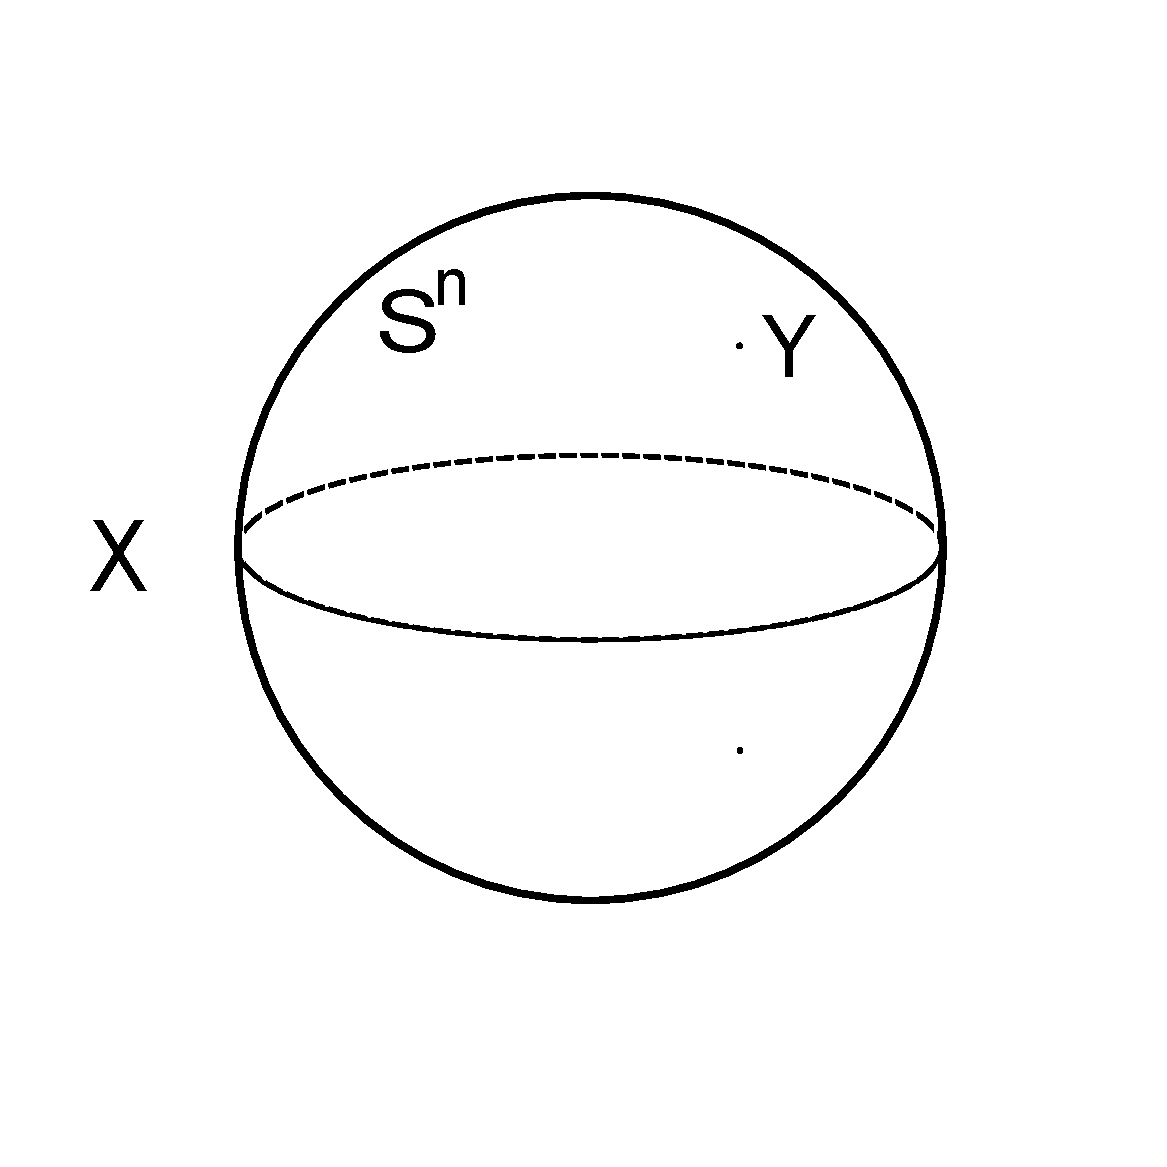
\includegraphics[width=0.2\textwidth]{figures/25.pdf}
%\caption{\small $X$ and $Y$ embedded in $S^n$.}
%\end{wrapfigure}
\subsection*{Alexander duality}
Let $X$ be a finite complex embedded in $S^n$; let $Y$ be another complex disjoint from $X$ in $S^k$. Fix a point $p$ not in $X$ or $Y$, and consider the stereographic projection $\textup{St}_p:S^n\setminus\{p\}\to\Rbb^n$.  Consider the map
\begin{cjointikzcd}
\diagram  X \times Y  \rar & S^{n-1}
%
\diagram \intertext{defined by}
%
\diagram (x, y)  \rar[mapsto] & \frac{\textup{St}_p(x)-\textup{St}_p(y)}{\|\textup{St}_p(x)-\textup{St}_p(y)\|}
\end{cjointikzcd}
%\begin{align*}
%X \times Y & \to S^{n-1} \\
%(x, y) & \mapsto \frac{x-y}{\|x-y\|}
%\end{align*}
and apply the Hopf construction to get a map
\begin{ctikzcd}
\Sigma(X\wedge Y)\rar["\simeq"] & X\ast Y \rar & S^n.
\end{ctikzcd}
In the category $\Scat$ we get a map $\fhat: X \sprod \Suspend^{1-n} Y \to S^0$.  Alexander duality says
\begin{thm}
If $Y \simeq S^n - X$ then $\fhat$ is a duality; $DX \simeq \Suspend^{1-n} Y$.
\end{thm}
\noindent The proof consists of showing that $\fhat/: \widetilde H_i (\Suspend^{1-n} Y) \xrightarrow{\cong} \widetilde H^i (X)$ is an isomorphism for $i \in \Zbb$.
\begin{rem}
If you think of $X$ and $Y$ as embedded in $\Rbb^n$ instead of $S^n$ and $Y \simeq \Rbb^n - X$, then $Y \simeq S^n - \Xpt$, so $D(\Xpt) \simeq \Suspend^{1-n} Y$.
\end{rem}

\subsection*{Milnor-Spanier duality}
%\begin{wrapfigure}{r}{0.3\textwidth}
%\centering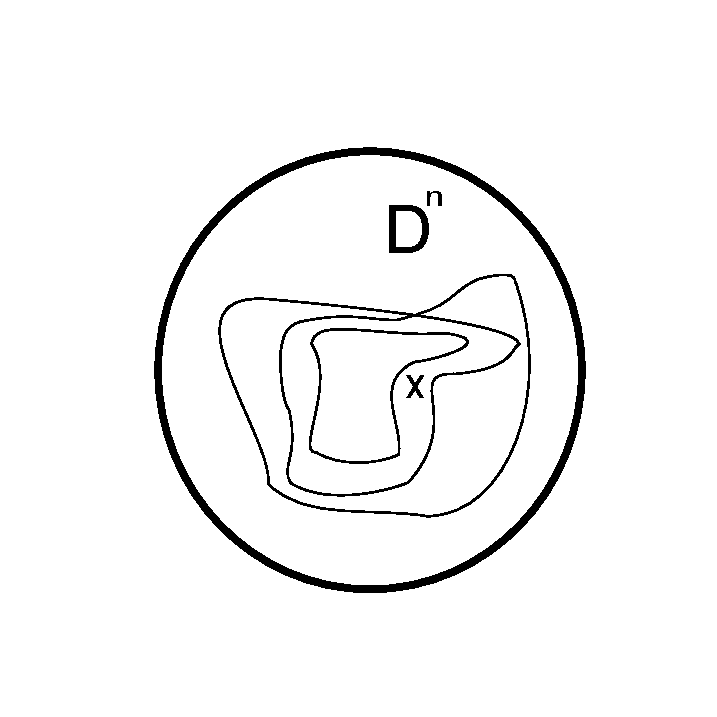
\includegraphics[width=0.2\textwidth]{figures/26.pdf}
%\caption{\small Set-up for Milnor-Spanier duality.}
%\end{wrapfigure}
Take $X \subseteq \mathrm{int}(D^n) \cong \Rbb^n$, and suppose $N \subseteq \mathrm{int}(D^n)$ is a regular neighborhood,\footnote{If you embed a finite complex into a Euclidean space, any sufficiently small
open neighborhood admits a deformation retraction back to the complex
 --- this is a `regular neighborhood'. If the complex is a manifold,
you can identify the normal bundle of the embedding with a regular
neighborhood. } so that the inclusion $X \xrightarrow{\simeq} N$ is a homotopy equivalence.  Then $D(\Xpt) \simeq \Suspend^{1-n}(D^n - N)$, by Alexander duality.
The virtue of the regular neighborhood is that you can identify what the suspension of the complement is: all you need to find the suspension is an inclusion into a contractible space, which we have, giving a degenerate cofiber sequence:
\begin{ctikzcd}
(D^n - N) \rar & D^n \rar &  D^n/(D^n - N) \rar["\simeq"] & \Suspend(D^n - N)\rar & \Sigma D^n
\end{ctikzcd}
Thus, as $D^n/(D^n-N)$ is homeomorphic to $\overline N/\partial\overline N$,
\[D(X_+)\simeq\Suspend^{1-n}(D^n - N) \simeq \Suspend^{-n}(D^n / (D^n-N)) \simeq \Suspend^{-n}(\bar N / \partial \bar N).\]
This is most useful when you can say something about $N$.  If $X$ is a $d$-dimensional manifold without boundary, then the normal bundle $\nu$ of the inclusion $X \into D$ is $(n-d)$-dimensional and $N$ is homotopy equivalent to the disk bundle of $\nu$.  It follows that $\bar N / \partial \bar N$ models the Thom complex $T (\nu)$, so $D(\Xpt) \simeq \Suspend^{-n} T(\nu) \simeq T(\nu - n \varepsilon)$.  This is called ``Milnor-Spanier duality'' (although it's not called that very often).  In (co)homology,
\[
E^{-i}(\Xpt) = E_i (D(\Xpt)) = E_{i+n} (T (\nu)).
\]
Observe also that $\nu + \tau = n \varepsilon$ where $\tau$ is the tangent bundle, so $D(\Xpt) = T(\nu - n \varepsilon) = T(-\tau)$, giving
\[
E^{-i}(\Xpt) = E_i (D(\Xpt)) = E_{i} (T (-\tau)).
\]
\subsection*{Poincar\'e duality}
If $\nu$ (or equivalently, $\tau$) is oriented for $E$ in the Milnor-Spanier setup, then the Thom isomorphism says $E_{i+n} (T (\nu)) \cong E_{i+d} (\Xpt)$. Thus:\footnote{More abstractly: the Thom isomorphism gives $E_{i-d}(T(-\tau))\cong E_i(X_+)$, and $E^{d-i}(X_+)\cong E_{i-d}(T(-\tau))$ by Milton-Spanier.}
\[E^{-i} (\Xpt) \cong E_{i+d} (\Xpt).\]
This gives standard Poincare duality, recalling that $E$ stands for the \emph{reduced} cohomology theory.

\subsection*{Atiyah duality}
%\begin{wrapfigure}[13]{r}{0.3\textwidth}
%\centering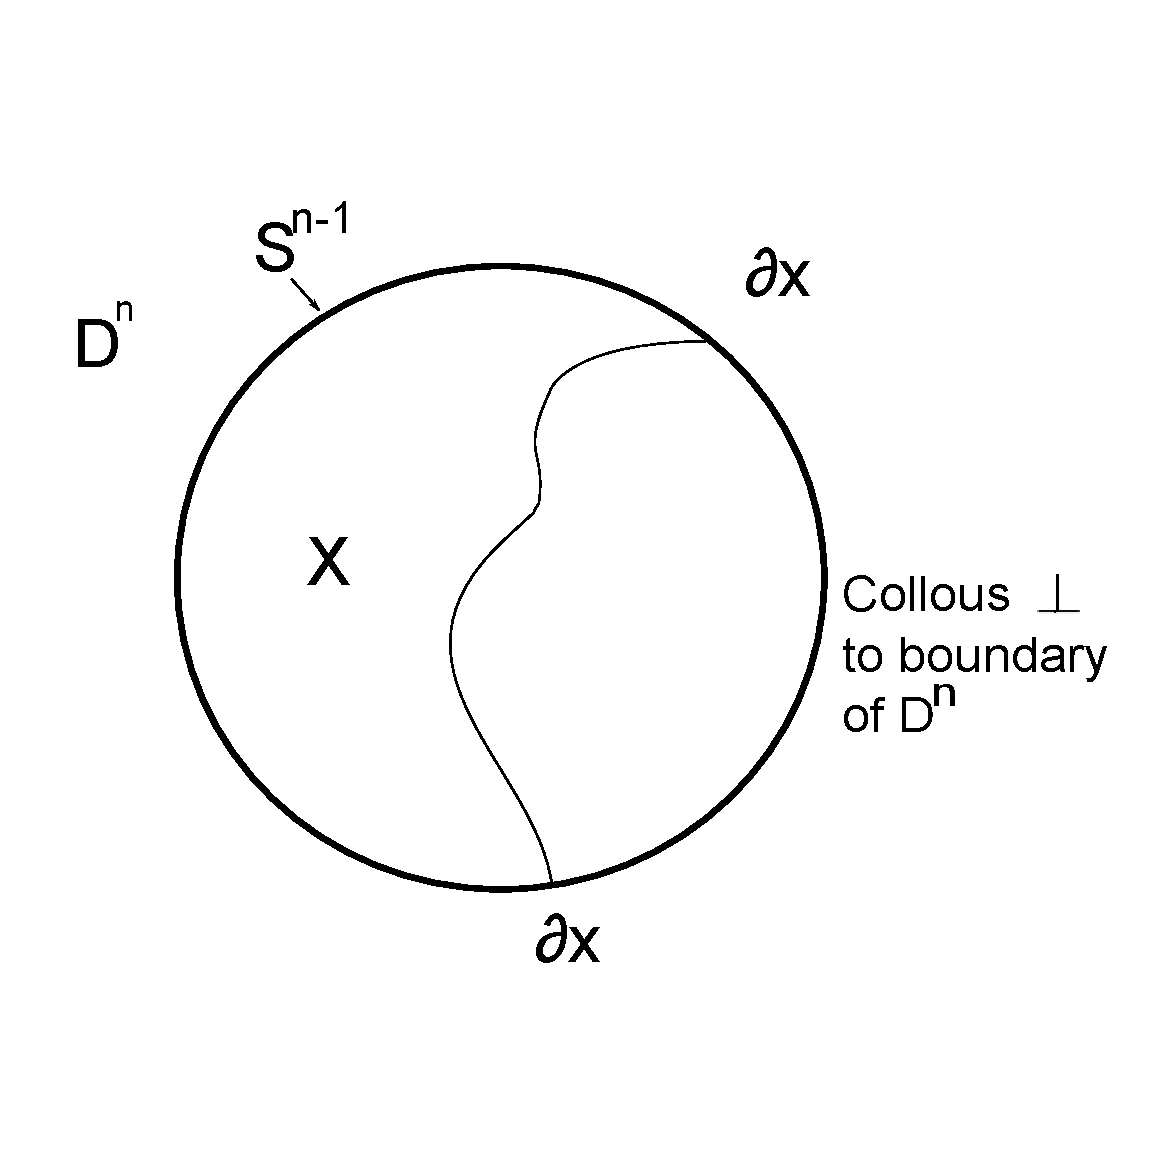
\includegraphics[width=0.3\textwidth]{figures/28.pdf}\vspace{-1cm}
%\caption{\small Diagram of Atiyah duality.}
%\end{wrapfigure}
This is a little mystical, so perhaps we should look at it more closely in the context of what's called Atiyah duality (for this, readers should look at Atiyah's exposition~\cite{Atiyah}).  Here we take for a change $(X, \partial X)$ to be a manifold with boundary.  You have to be careful about interpreting the tangent bundle of a manifold with boundary; $\tau_X$ is best defined to be $d$-dimensional everywhere, but with an identified $(d-1)$-dimensional subbundle on the boundary.  %Referencing the figure, this isn't quite what we had before.

Now suppose that $X$ is embedded in $D^n$ such that $\partial X$ lies in $\partial D^n=S^{n-1}$, and moreover that $X$ is transverse to $S^{n-1}$ wherever they coincide. Suppose also that $N$ is an open neighborhood of $X$ in $D^n$ such that $N\cap S^{n-1}$ is a regular open neighborhood of $\partial X$ in $S^{n-1}$. Then, we take the cone on this situation, as in figure \ref{AtiyahDuality}.
\begin{figure}[ht!]
\centering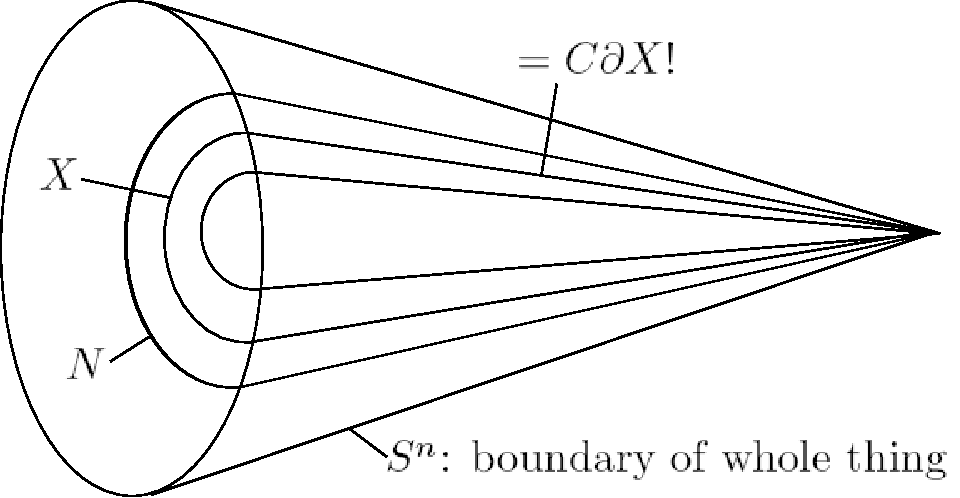
\includegraphics[width=0.4\textwidth]{figures/figure29.pdf}
\caption{\small Atiyah duality.}\label{AtiyahDuality}
\end{figure}

Now, $X / \partial X$ is homotopic to  $Y = X \cup C \partial X$, which is a subcomplex of $\partial(CD^n)\cong S^n$.  Moreover, $Y$ has $N \cup C(N \cap S^{n-1})$ as a regular neighborhood in $S^n$, and its complement is $K=S^n - (N \cup C(N \cap S^{n-1}))$.  Finally, $K$ deformation retracts onto $(D^n-N)$, as the tip of the cone does not lie in $K$. So, applying Alexander duality to $Y\subseteq S^n$ gives
\begin{align*}
D(X / \partial X) & \simeq D(Y) \\
& \simeq \Suspend^{1-n}(K) \\
& \simeq \Suspend^{1-n}(D^n - N) \\
& \simeq \Suspend^{-n}(\bar N / \partial \bar N) \\
& \simeq \Suspend^{-n} T (\nu)\\
& = T(-\tau),
\end{align*}
and this is Atiyah duality.

Now suppose $X$ is a compact closed manifold and $\xi \downarrow X$ is a smooth vector bundle; then $(D(\xi), S(\xi))$ is a compact manifold with boundary.  Atiyah duality says
\begin{align*}
D(T(\xi))
& \simeq T(-\tau_{D(\xi)}) \\
& \simeq T(-\pi^*(\tau_X \oplus \xi)) \\
& = T(-\tau_X - \xi),
\end{align*}
where $\pi$ is the projection $D(\xi) \to X$ (a homotopy equivalence).
\subsection*{Lefschetz duality}
Now suppose that $X$ is oriented for $E$, i.e., that there is a Thom isomorphism $E_i(X_+)\cong E_{i-d}(T(-\tau))$. Then from Atiyah duality we derive Lefschetz duality: $E_i (X_+) \simeq E^{d-i}(X, \partial X)$.
\subsection*{Stunted projective space}
Here's an example: take $X = \RP^{k-1}$ and $\xi = n \bundle{L}$. % (we'll take $n \ge 0$ for the moment; we'll see it doesn't make any difference soon).
Then, we saw in lecture \ref{BuildingThomSpaces} (at least for $n\geq0$) that \[T(n \bundle{L}) = \RP^{n+k-1} / \RP^{n-1} =: \RP^{n+k-1}_n.\]
More generally, we can define, whenever $t+b\geq1$:
\[\RP^{t-1}_{-b}:= T(-bL\downarrow\RP^{t+b-1}),\]
a spectrum with cells in every dimension from $-b$ to $t-1$, inclusive.

Moreover, it happens\footnote{To see this, one argues as follows. View $\bundle{L}$ as a subbundle of $\RP^{k-1}\times \Rbb^k$, where $\RP^{k-1}$ is viewed as the set of lines $\Rbb\{x\}$ in $\Rbb^k$, for nonzero $x\in\Rbb^k$. Then we can produce a bundle isomorphism $\Hom(\bundle{L},\bundle{L}^\perp)\to\tau(\RP^{k-1})$ by sending $h:\Rbb\{x\}\to \Rbb\{x\}^\perp$ to the germ at $0$ of the path $t\mapsto \Rbb\{x+t\cdot h(x)\}$ in $\RP^{k-1}$. Noting that $\Hom(\bundle L,\bundle L)$ is a line bundle with a nonvanishing section, it is trivial, so $\tau(\RP^{k-1})+\Rbb=\Hom(\bundle L,\bundle L^\perp\oplus\bundle L)=\Hom(\bundle L,\Rbb^k)=\Hom(\bundle L,\Rbb)^k=\bundle L^k$.}\todo{I find this footnote very hard to read.} that $\tau(\RP^{k-1}) + \varepsilon = k \bundle{L}$.
%\begin{enumerate}
%\item $T(n \bundle{L}) = \RP^{n+k-1} / \RP^{n-1} \simeq \RP^{n+k-1}_n$, (see lecture); and
%\item $\tau(\RP^{k-1}) + \varepsilon = k \bundle{L}$.\footnote{To see this, one argues as follows. View $\bundle{L}$ as a subbundle of $\RP^{k-1}\times R^k$, where $\RP^{k-1}$ is viewed as the set of lines $\Rbb\{x\}$ in $\Rbb^k$, for nonzero $x\in\Rbb^k$. Then we can produce a bundle isomorphism $\Hom(\bundle{L},\bundle{L}^\perp)\to\tau(\RP^{k-1})$ by sending $h:\Rbb\{x\}\to \Rbb\{x\}^\perp$ to the germ at $0$ of the path $t\mapsto \Rbb\{x+t\cdot h(x)\}$ in $\RP^{k-1}$. Noting that $\Hom(\bundle L,\bundle L)$ is a line bundle with a nonvanishing section, it is trivial, so $\tau(\RP^{k-1})+\Rbb=\Hom(\bundle L,\bundle L^\perp\oplus\bundle L)=\Hom(\bundle L,\Rbb^k)=\Hom(\bundle L,\Rbb)^k=\bundle L^k$.}
%\end{enumerate}
By Atiyah duality, $D(T(n\bundle{L})) \simeq T(-n \bundle{L} - \tau)$, so that
\[D(\RP^{n+k-1}_n) = D(T(n\bundle{L})) \simeq T(-n \bundle{L} - \tau) = T(-n \bundle{L} + \varepsilon -k \bundle{L}) = \Suspend T(-(n+k)\bundle{L}) =: \Suspend \RP^{-n-1}_{-n-k}.\]
Summarizing:
\[D(\RP^{t-1}_{-b}) \simeq \Suspend (\RP^{b-1}_{-t})\text{ for }t+b\geq1.\]
% $D(\RP^{t-1}_{-b}) \simeq \Suspend \RP^{b-1}_{-t}$, for $b, t \in \Zbb$, $t-1 \ge -b$ (and taking $b = -n$, $t = n+k$ in the above.  The condition $t-1 \ge -b$ requires that $\RP^{t-1}_{-b}$ has a cell.) or $\RP^{t-1}_b = T(-b \bundle{L} \downarrow \RP^{t+b-1})$.

By the way, if you don't like these somewhat ethereal spaces, you can use James Periodicity: let $a$ be the periodicity of $\bundle{L}$ in $\widetilde J(\RP^{t+b-1})$.  Then $T((ja-b)\bundle{L}) \simeq \Suspend^{ja} T(-b \bundle{L})$; for $j$ big enough, $T((ja-b)\bundle{L})$ is an actual stunted projective space!

% >>>
\fi
\BoxedNote{}












\section{The structure of stunted projective space} % <<<
\label{TheStructureOfStuntedProjectiveSpace}
\ifx\OutputTheStructureOfStuntedProjectiveSpace\undefined\else
Today we look at the attaching maps for stunted projective spaces.  In fact, the attaching maps we're going to look at are the ``stable relative attaching maps,'' so perhaps we should begin by saying what that means.  Suppose $X$ is a CW complex; then it has a skeletal filtration $\Sk_* (X)$.  The $(k+1)$-skeleton is obtained from the $k$-skeleton by attaching $(k+1)$-cells as in the following pushout square:
\begin{ctikzcd}
\Sk_k (X) \rar[hook] & \Sk_{k+1} (X) \\
\bigvee S^k \uar\rar[hook] & \bigvee D^{k+1}\uar.
\end{ctikzcd}
Although the attaching maps $S^k \to \Sk_k (X)$ are to the $k$-skeleton, it's certainly possible that an attaching map pulls back to a lower skeleton.  A ``relative attaching map'' for a $(k+1)$-cell (attached via $r$) is a factorization of this kind through the lowest possible skeleton; that is, the map $a'$ below:
\begin{ctikzcd}[column sep=large]
\Sk_{k-j-1} (X) \rar[into] & \Sk_{k-j} (X)  \rar[hook,"\cdot\,\cdot\,\cdot" description] & \Sk_k (X) \rar[into] & \Sk_{k+1} (X)\\
&S^k\ular[dashed,"\nexists" scale=1.5]\uar["a'"]\urar[yshift=0.2em,"r"]\rar[into]&\bigvee S^k\uar\rar[into]&\bigvee D^{k+1}\ar[u]
\end{ctikzcd}
A ``stable relative attaching map'' is a stable one of these.  That is, the cells of the $(k+2)$-skeleton of $\Suspend X$ are the suspension of the cells of the $(k+1)$-skeleton of $X$,
so one could ask how far down an attaching map factors, perhaps after suspending very often (ignoring the wavy arrow for the moment):
\begin{ctikzcd}[column sep=large, decoration={markings, mark connection node=dots, mark=at position .5 with {\node (dots) {$\cdots$};}}]
&\bigvee S^{k-j+n}\mathrlap{=C(\imath)}\\
\Sk_{k-j+n-1} (X) \rar[into] & \Sk_{k-j+n} (X) \uar[wavy,"b"'] \rar[hook,"\cdot\,\cdot\,\cdot" description] & \Sk_{k+n} (X) \rar[into] & \Sk_{k+n+1} (X)\\
&S^{k+n}\ular[dashed,"\nexists" scale=1.5]\ar[u,"a'"]\urar[yshift=0.1em,"r"]\rar[into]&\bigvee S^{k+n}\uar\rar[into]&\bigvee D^{k+n+1}\ar[u]
\end{ctikzcd}
The inclusion $\imath$ of one skeleton in the next is a cofibration, and stably, the corresponding cofibration sequence (drawn with the wavy arrow $b$) is also a fibration sequence.
Thus, if $a$ does not factor stably through a lower skeleton the composite $ba$ defines a nonzero element of $\pi_{k+n}^S \left( \bigvee S^{k-j+n} \right) = \bigoplus \pi_j^S$.\footnote{Warning: there's indeterminacy in how you factor the attaching map, so the element you get may not be well-defined.}

In any case, we want to understanding the stable relative attaching maps for $\RP^\infty$ using the standard cell structure, with one cell in each dimension. We'll format the diagrams a little differently now. Let $\pi$ be the attaching map for a particular cell in dimension $k$  and let $c$ be the collapse map from $\RP^{k-j}$ onto its top cell.

In the following diagram we ask for the largest value of $j$ such that the stable attaching map factors, and also what the compression $c\overline\pi$ of the stable attaching map onto the top cell is as an element of $\pi^S_j$.
\begin{ctikzcd}[column sep = 4.5em,row sep=2.3em]
\RP^{k-j-1}\ar[from=drrr,dashed,"\nexists" {very near end, scale=1.5}]\rar[hook,"\imath"] & \RP^{k-j}\dar[crossing over, "c"' pos=0.6]\rar[hook,"\cdot\,\cdot\,\cdot" description] & \RP^k \rar[hook] & \RP^{k+1}\\
&S^{k-j}&&\ar[ull,"\overline\pi"' pos=0.53]S^{k}\ar[ul,"\pi"']\ar[ll,"c\overline\pi"]
\end{ctikzcd}

%\begin{ctikzcd}[row sep=large, column sep = 4em]
%\RP^{k-j-1}\ar[from=drr,dashed,"\nexists" {near end, scale=1.5}]\rar[hook,"\imath"] & \RP^{k-j}\dar[crossing over,"c" pos=0.4]\rar[hook,] & \RP^k \rar[hook] & \RP^{k+1}\\
%&S^{k-j}&\ar[ul,"\overline\pi"']S^{k}\ar[u,"\pi"']\ar[l,"c\overline\pi"]
%\end{ctikzcd}

The answer will come out in terms of the image of the $J$-homomorphism --- actually its stable version $j: \pi_{*-1}(O) \to \pi_{*-1}(QS^0) = \pi_{*-1}^S$.  Remember $\pi_{*-1}(O) = \pi_* (BO) = \KOtwee^{-*}$.  Here's a table, leaving out degrees where $\KOtwee^{-*} = 0$:

\[
\begin{array}{cc|ccl}
i=\nu(2^i) & *=\rho(2^i) & \KOtwee^{-*}=\pi_{*-1}(O) &&j_i:=j(g_i)\in\pi_{*-1}^S \\
\hline
0 & 1 & {\Zbb_2 \anglebrace{g_0}} && j_0=-2 \iota \\
1 & 2 & {\Zbb_2 \anglebrace{g_1}} && j_1=\eta \\
2 & 4 & {\phantom{_2}\Zbb \anglebrace{g_2}} && j_2=\nu\ %\{
\smash{\Biggr \}
\raisebox{-1.1ex}{\small\shortstack{Hopf invariant\\one elements}}}\\
3 & 8 & {\phantom{_2}\Zbb \anglebrace{g_3}} && j_3=\sigma \\
4 & 9 & {\Zbb_2 \anglebrace{g_4}} && j_4=\eta \sigma \\
5 & 10 & {\Zbb_2 \anglebrace{g_5}} && j_5=\eta^2 \sigma
\end{array}
\]

Implicit in the organization of this table is the observation that the coefficient groups $\KOtwee^{-*}$ are all cyclic, and nonzero only when $*=\rho(2^e)$. Thus we write $g_i$ for a generator of the $(i+1)^\text{st}$ nonzero coefficient group, and $j_i$ for its image $j(g_i)$ under the stable $J$-homomorphism.

Note that $g_0$ has order two, but $j_0:=j(g_0)$ has infinite order, so that $j:\pi_0(O)\to\pi^S_0$ cannot be a homomorphism. However, it is a homomorphism in higher degrees.\todo{This remark will go away when we replace $QS^0$ with $BGL_1 \Sbb^0$.}

Our discussion of the attaching maps will begin where the answer is, which may seem like a funny place at first, so have patience.  Recall the following facts:
\[\KOtwee(\RP^k)=\Zbb_{a_k}\anglebrace{\bundle L-1},\text{ defining }\begin{array}{c|cccccccc}
k&0&1&2&3&4&5&6&7\\\hline
a_k&1&2&4&4&8&8&8&8
\end{array}\text{ and }a_{k+8}=16a_k,\]
so that, $a_k|n$ exactly when $k\leq\rho(n)-1$. Thus when $k = \rho(n) - 1$ we have $a_k=2^{\nu(n)}$ and $a_{k+1}=2^{\nu(n)+1}$. Just to reiterate the above, this gives
\begin{align*}
\KOtwee \left( \RP^{\rho(n) - 1} \right) & = \Zbb_{2^{\nu(n)}} \anglebrace{\bundle L - 1 } \\
\KOtwee \left( \RP^{\rho(n)} \right) & = \Zbb_{2^{\nu(n) + 1}} \anglebrace{\bundle L - 1 }.
\end{align*}
Now note that $\imath^*(\bundle L)=\bundle L$, where $i$ is the inclusion in the cofiber sequence
\begin{tikzcd}[column sep=scriptsize]
\RP^{\rho(n) - 1} \rar[into,"\imath"]& \RP^{\rho(n)} \ar[r,"b"]& S^{\rho(n)}
\end{tikzcd}.
We then examine the exact sequence
\begin{ctikzcd}
\KOtwee \left( \RP^{\rho(n) - 1} \right) & \lar["\imath^*"'] \KOtwee \left( \RP^{\rho(n)} \right) & \lar["b^*"'] \KOtwee (S^{\rho(n)})\\
\Zbb_{2^{\nu(n)}} \anglebrace{\bundle L - 1 }\uar[equal] & \lar[onto,"\imath^*"']\Zbb_{2^{\nu(n) + 1}} \anglebrace{\bundle L - 1 }\uar[equal] & \lar["b^*"']\anglebrace{g_{\nu(n)}}\uar[equal].
\end{ctikzcd}
By exactness, $b^*(g_{\nu(n)})=2^{\nu(n)}(\bundle L - 1)=n(1-\bundle L)$, the nonzero element\footnote{Notice that in $\Zbb_{2^{\nu(n) + 1}} \anglebrace{\bundle L - 1}$, $2^{\nu(n)}(\bundle L - 1)$ is congruent to any of its odd multiplies, and $-n$ is an odd multiple of $2^{\nu(n)}$.} of $\ker(\imath^*)\simeq\Zbb_2$.
%That is $b^*(g_{\nu(n)})=n(\bundle L-1)$.

In terms of bundles, this means that $n(1-\bundle L)$ over $\RP^{\rho(n)}$ is classified by a map into $BO$ that factors as $b$ followed by $g_{\nu(n)}$:
\begin{center}
\begin{tikzcd}
\ar[d]n(1-\bundle L) \ar[r] & E(g_{\nu(n)})\ar[d] \\
\RP^{\rho(n)}\rar["b"] & S^{\rho(n)} \rar["g_{\nu(n)}"] & BO
\end{tikzcd}
%
\quad
%
\sbox0{\Bullet $E(g_{\nu(n)})$ is the virtual bundle classified by $g_{\nu(n)}$}
\begin{minipage}{\wd0}
\Bullet $E(g_{\nu(n)})$ is the virtual bundle classified by $g_{\nu(n)}$

\Bullet $H^{\rho(n)}(b;\Zbb_2)$ is an isomorphism
\end{minipage}
%
%\fbox{\begin{minipage}{5cm}
%\Bullet $E(g_{\nu(n)})$ is the virtual bundle classified by $g_{\nu(n)}$
%
%\Bullet $H^{\rho(n)}(b;\Zbb_2)$ is an isomorphism
%\end{minipage}}
\end{center}
That's the starting point.  Now we study the Thom spaces to get stunted projective spaces.  In the $\Scat$-category, we have a map on Thom spaces (relative to $S^0$):
\begin{ctikzcd}
S^0 \dar\rar[equal] & S^0\dar\\
\Suspend^n\!\left(\RP^{\rho(n)-n}_{-n}\right)\rar["\btwee"] & T\!\left(g_{\nu(n)}\right)
\end{ctikzcd}

The first question is: ``what is $T(g_{\nu(n)})$?''  By the Thom isomorphism, $T(g_{\nu(n)})$ has a 0-cell and a $\rho(n)$-cell; the attaching map is an element of $\pi_{\rho(n)-1} (Q S^0)$.
\begin{thm}
The attaching map for $T(g_{\nu(n)})$ is $j_{\nu(n)} = j(g_{\nu(n)}) \in \pi_{\rho(n)-1}(QS^0)$.
\end{thm}
This almost has the status of a folk theorem; it's due to Toda and Adams.  We will prove it next time; for now, what else could it be?  Now we can line up two cofiber sequences vertically:
\begin{ctikzcd}
S^0 \dar\rar[equal] & S^0\dar\\
\Suspend^n\!\left(\RP^{\rho(n)-n}_{-n}\right)\dar\rar["\btwee"] & T\!\left(g_{\nu(n)}\right)\dar\\
\Suspend^n\!\left(\RP^{\rho(n)-n}_{-n+1}\right)\rar["c"] & S^{\rho(n)}
\end{ctikzcd}
Now $\Suspend^n (\RP^{\rho(n)-n}_{-n+1})$ has a cell in each dimension from 1 to $\rho(n)$ inclusive. By naturality of the Thom isomorphism $H^{\rho(n)}(\widetilde b;\Zbb_2)$ is an isomorphism in dimension $\rho(n)$,  so the 5-lemma implies that $H^{\rho(n)}(c;\Zbb_2)$ is also an isomorphism, and $c$ is the collapse map (up to sign).
\ConfusedBox{Must we localize at two to assert this about $c$?}
In other words, $\Suspend^n \RP^{\rho(n)-n}_{-n}$ has cells between dimensions $0$ and $\rho(n)$, and the map to $T(g_{\nu(n)})$ strips away the cells in between.
\begin{figure}[h!]
\centering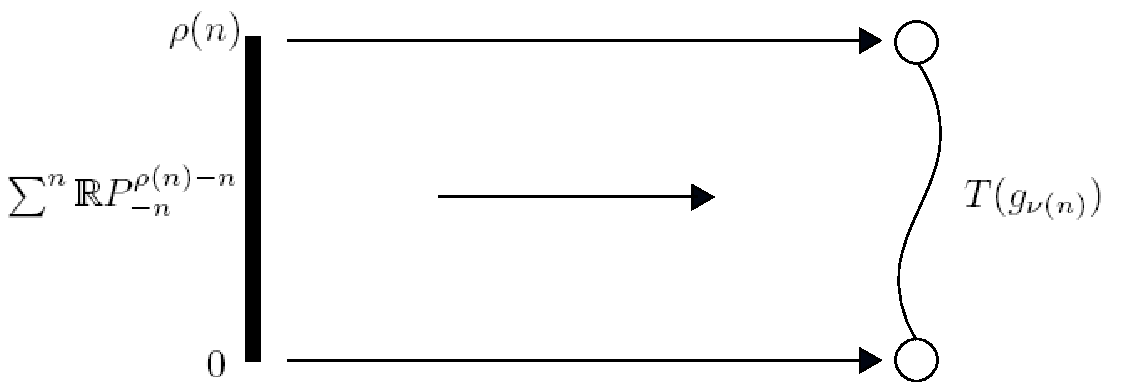
\includegraphics[width=0.4\textwidth]{figures/figure30.pdf}
\caption{\small Picture of the map $\widetilde b$.}
\end{figure}

Well that's pretty good, only attaching maps are supposed to go the other way, so let's dualize this picture.  Two facts about the Spanier-Whitehead dual we will use are that $D \RP^{t-1}_{-b} = \Suspend \RP^{b-1}_{-t}$ (see lecture \ref{Dualities}), and that the dual $D(f)$ of $f:S^p\to S^0$ is $\pm\Sigma^{-p}f:S^0\to S^{-p}$.

The only space whose dual we have left to compute is $T(g_{\nu(n)})$.  Since by the folk theorem $T(g_{\nu(n)}) = C(j_{\nu(n)})$ we have a cofiber sequence
\begin{tikzcd}[column sep=normal]
S^{\rho(n)-1} \rar["j_{\nu(n)}"] & S^0 \rar& T(g_{\nu(n)}).
\end{tikzcd}
Continuing the dual cofiber sequence:
\begin{ctikzcd}
\Sigma^{-\rho(n)+1}T(g_{\nu(n)}) & \lar S^{-\rho(n)+1}
&[-\columnsep+1em+width("${}^{\pm\Sigma^{-\rho(n)+1}j_{\nu(n)}}$")]
\lar["\pm\Sigma^{-\rho(n)+1}j_{\nu(n)}"'] S^0 & \lar D(T(g_{\nu(n)}))
\end{ctikzcd}
Thus $D(T(g_{\nu(n)}))=\Suspend^{-\rho(n)}T(g_{\nu(n)})$, so $T(g_{\nu(n)})$ is nearly self-dual. In particular, we can now write down the dual diagram to that drawn above\todo{Make it more explicit which diagram above.} (at left) and its $(n-1)$-fold suspension (at right):
\begin{cjointikzcd}[sep=large]
\diagram
    S^0 \rar[equal] & S^0\\
    \Sigma^{1-n}\RP^{n-1}_{n-\rho(n)-1}\uar& \lar["D\btwee"'] \Sigma^{-\rho(n)}C\left(j_{\nu(n)}\right)\uar\\
    \Sigma^{1-n}\RP^{n-2}_{n-\rho(n)-1}\uar & \lar["Dc"' pos=0.67] S^{-\rho(n)}\uar\\
    S^{-1}\uar \rar[equal] & S^{-1}\uar["\Sigma^{-\rho(n)}j_{\nu(n)}"]
%
\diagram
    S^{n-1} \rar[equal] &[width("$C\left(j_{\nu(n)}\right)$")] S^{n-1}\\
    \RP^{n-1}_{n-\rho(n)-1}\uar&\lar["\Sigma^{n-1}D\btwee"'] \Sigma^{n-\rho(n)-1}\edgerlap{C\left(j_{\nu(n)}\right)}\uar\\
    \RP^{n-2}_{n-\rho(n)-1}\uar & \lar["\Sigma^{n-1}Dc"'] S^{n-\rho(n)-1}\uar\\
    S^{n-2}\uar \rar[equal] & S^{n-2}\uar["\Sigma^{n-\rho(n)-1}j_{\nu(n)}"]
\end{cjointikzcd}
\todo[noline]{I think we should suppress the suspensions from the arrow names in the righthand diagram.}
Here, $\pi$ is the attaching map for $\RP^{n-2}_{n-\rho(n)-1} \to \RP^{n-1}_{n-\rho(n)-1}$; this follows because the columns are cofiber sequences. Moreover, as $\Sigma^{n-1} Dc$ is dual to the collapse map (up to sign), it is the inclusion of the bottom cell (up to sign). %  The map $j_{\nu(n)}$ might look funny, but it works out because we're dealing with spectra.
Well so we've done it: we've factored $\pi$ as $j_{\nu(n)}$ followed by inclusion of the bottom cell.
\begin{ctikzcd}
S^{n-2}\drar["j_{\nu(n)}"] \rar["\pi"] & \RP^{n-2}_{n-\rho(n)-1} \\
& S^{n-\rho(n)-1}\uar
\end{ctikzcd}
In other words, the attaching map for the top cell of $\RP^{n-1}_{n-\rho(n)-1}$ pulls all the way back to the $(n-\rho(n)-1)$-skeleton.  It goes no further: that would mean that $\pi \simeq \ptspace$, but if $\pi$ were stably nullhomotopic, then the top cell of $\RP^{n-1}_{n-\rho(n)-1}$ would stably split off. Dualizing, the bottom cell $S^0$ of $\Suspend^n \RP^{\rho(n)-n}_{-n} = T(n(1-\bundle L) \downarrow \RP^{\rho(n)})$ would split off, which would then imply that $n(1-\bundle L)$ would be stably fiber homotopy trivial. This is of course not the case, by the solution to the vector fields problem --- $\widetilde J (\RP^{\rho(n)}) = \Zbb_{2^{\nu(n)+1}} \anglebrace{\bundle L - 1 }$.

\ConfusedBox{\textbf{For some reason I find this a bit confusing. I've put in an alternative.} It goes no further: that would mean that $\pi \simeq \ptspace$, but if $\pi$ is stably nullhomotopic then we'd get
\begin{ctikzcd}[ampersand replacement=\&]
\& \& S^0\dlar["\exists"]\dar["\id"] \\
\Suspend^{-n+1} \RP^{n-2}_{n - \rho(n) - 1} \rar \& \Suspend^{-n+1} \RP^{n-1}_{n-\rho(n)-1} \rar \& S^0 \rar["\pi"] \& \Suspend^{-n+2} \RP^{n-2}_{n-\rho(n)-1},
\end{ctikzcd}
because the sequence is an exact triangle, a map going back as above.  Looking at what that means in terms of the dual, it means there is a stable splitting of the $0$-sphere \begin{tikzcd}[ampersand replacement=\&,column sep=scriptsize]
S^0 \rar[yshift=0.2em] \& \lar[yshift=-0.2em] \Suspend^n \RP^{\rho(n)-n}_{-n} = T(n(1-\bundle L) \downarrow \RP^{\rho(n)})
\end{tikzcd} which would mean that $n(1-\bundle L)$ is stably fiber-homotopy trivial, equivalently that $n\bundle L$ is stably fiber-homotopy trivial.  But by the vector field problem, it's not: $n(1-\bundle L) \ne 0$ in $\widetilde J \RP^{\rho(n)} = \Zbb_{2^{\nu(n)+1}} \anglebrace{\bundle L - 1 }$.
}
Now it's an easy matter to get back to the general case: consider $\RP^{n-1}_{-N}$, where $-N \leq n - \rho(n) - 1$.\footnote{The quantity $n - \rho(n) - 1$ is $-1$ when $n=1,2,4,8$, and positive for other $n>0$.}   Then we have a diagram with the bottom row a cofiber sequence (drawn at left):
\begin{cjointikzcd}[intertext,row sep=tiny]
\diagram
& \RP^{n-2}_{-N}\rar["\text{coll}" pos=0.65] & \RP^{n-2}_{n-\rho(n)-1}\\
\RP^{n-\rho(n)-2}_{-N} \rar[into]   & \RP^{n-\rho(n)-1}_{-N} \rar["\text{coll}" pos=0.45] \uar[hook] & S^{n-\rho(n)-1}\uar[hook]
%
\diagram[1em] \intertext{Applying $\pi_{n-2}^S(\text{---})$:}
%
\diagram[-8em] % There seems to be a bug in cjointikzcd.
& \pi\rar[mapsto] & \pi\\
? \rar[mapsto,dashed] & \overline\pi \rar[mapsto]\uar[mapsto] & j_{\nu(n)}\uar[mapsto]
\end{cjointikzcd}
From what we had before, the attaching map $\pi:S^{n-2}\to\RP^{n-2}_{-N}$ pulls back stably to a map $\overline\pi:S^{n-2}\to\RP^{n-\rho(n)-1}_{-N}$, whose compression onto the top cell $S^{n-\rho(n)-1}$ is $j_{\nu(n)}\neq0$. Thus, applying $\pi_{n-2}^S$ to the above diagram, we have elements as in the box at the right. As $j_{\nu(n)}$ is nonzero, and the bottom row is exact ($\pi_*^S$ is a homology theory) there can be no element of $\pi_{n-2}^S(\RP^{n-\rho(n)-2}_{-N})$ mapping to $\overline \pi$.
Thus:
\begin{thm}\label{RelAttachThm}
The stable relative attaching map for the $(n-1)$-cell of $\RP^{n-1}_{-N}$ can be taken to be $j_{\nu(n)}$; that is, stably, there is some $\overline \pi$ which does not pull back any further stably, and so that $c\overline\pi=j_{\nu(n)}$:
\begin{ctikzcd}[column sep = 4.5em,row sep=2.3em]
\RP^{n-\rho(n)-2}_{-N}\rar[hook,"\imath"] & \RP^{n-\rho(n)-1}_{-N}\latearrow[crossing over, "c"' pos=0.6]\rar[hook,"\cdot\,\cdot\,\cdot" description] & \RP^{n-2}_{-N}  \rar[hook] & \RP^{n-1}_{-N} \\
&S^{n-\rho(n)-1}&&\ar[ulll,dashed,"\nexists" {very near end, scale=1.5}]\ar[ull,"\overline\pi"' pos=0.53]S^{n-2}\ar[ul,"\pi"']\ar[ll,"j_{\nu(n)}"]
\end{ctikzcd}\todo[noline]{Fix the notation so that this diagram has roughly the same names as the very similar ones back a few pages. The previous set of diagrams use $k=n+2$ in place of $n$.}
%\[\xymatrix@!0@C=3.5cm@R=1.4cm{
%\RP^{n-\rho(n)-2}_{-N}\ar@{^{(}->}[r]^\imath &\ar[d] \RP^{n-\rho(n)-1}_{-N}\ar|{\ \cdot\ \cdot\ \cdot\ }@{^{(}->}[r]& \RP^{n-2}_{-N} \ar@{^{(}->}[r] & \RP^{n-1}_{-N}\\
%&\makebox[0cm][r]{$C(\imath)=$\,}S^{n-\rho(n)-1}&\ar@{^{(}->}[r]\ar[ul]_{\overline\pi}\ar@{-->}[ull]^(.75){\text{\large$\nexists$}}S^{n-2}\ar@{^{(}->}[r]\ar[u]^\pi\ar[l]^{j_{\nu(n)}}&D^{n-1}\ar[u]
%}\]
\end{thm}

It's time to draw some pictures. First, here are the stable relative attaching maps in $\RP^\infty_{-1}$:
\begin{center}
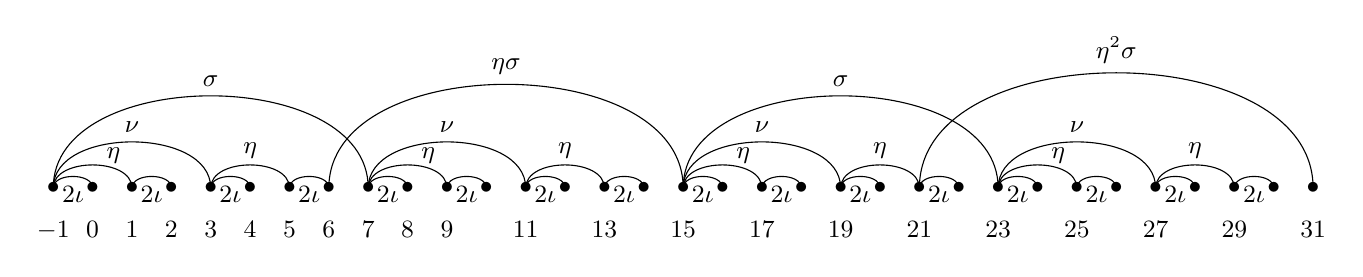
\begin{tikzpicture}[
    scale=0.5, font=\small,
    every path/.append style={out=90,in=90},
    every node/.append style={execute at begin node=$,execute at end node=$},
    every edge quotes/.style={auto=right}
]
    \foreach \x in {-1,...,9,11,13,...,31}
        \node[below] at (\x,-.6) {\x};
    \foreach \x in {-1,...,31}
        \node at (\x,0) {\Bullet};
    \foreach \x in {0,2,...,30}
		\draw (\x,0) to["2\iota"'] (\x-1,0);
    \foreach \x in {1,9,...,25}
		\draw (\x,0) to["\eta" {pos=0.465, yshift=-0.7ex}]   (\x-2,0);
    \foreach \x in {5,13,...,29}
		\draw (\x,0) to["\eta" yshift=-0.3ex]  (\x-2,0);
    \foreach \x in {3,11,...,27}
		\draw (\x,0) to["\nu"] (\x-4,0);
    \foreach \x in {7,23}
		\draw (\x,0) to["\sigma"]  (\x-8,0);
    \foreach \x in {15}
		\draw (\x,0) to["\eta\sigma"]  (\x-9,0);
    \foreach \x in {31}
		\draw (\x,0) to["\eta^2\sigma"]  (\x-10,0);
\end{tikzpicture}
\end{center}
%\begin{center}
%\begin{tikzpicture}[scale=.95]
%    \foreach \x in {-1,...,9,11,13,...,31}
%        \path (.5*\x,-.3) node[below] {\x};
%    \foreach \x in {-1,...,31}
%        \path (.5*\x,0) node {$\Bullet$};
%    \foreach \x in {0,2,...,30}
%		\draw[->] (.5*\x,0) to[out=90,in=90] node[below] {\small$2\iota$}  (.5*\x-.5,0);
%    \foreach \x in {1,5,...,29}
%		\draw[->] (.5*\x,0) to[out=90,in=90] node[right] {\small$\,\ \eta$}  (.5*\x-1,0);
%    \foreach \x in {3,11,...,27}
%		\draw[->] (.5*\x,0) to[out=90,in=90] node[above] {\small$\nu$}  (.5*\x-2,0);
%    \foreach \x in {7,23}
%		\draw[->] (.5*\x,0) to[out=90,in=90] node[below] {\small$\sigma$}  (.5*\x-4,0);
%    \foreach \x in {15}
%		\draw[->] (.5*\x,0) to[out=90,in=90] node[below] {\small$\eta\sigma$}  (.5*\x-4.5,0);
%    \foreach \x in {31}
%		\draw[->] (.5*\x,0) to[out=90,in=90] node[below] {\small$\eta^2\sigma$}  (.5*\x-5,0);
%\end{tikzpicture}
%\end{center}


%\begin{figure}[h!]
%\centering\includegraphics[width=0.8\textwidth]{figures/fig31fix.png}
%\caption{\small Stable relative attaching maps in $\RP^\infty_{-1}$.}
%\end{figure}

For example, if $n$ is odd then $\rho(n) = 1$, $\nu(n) = 0$.  So the attaching map for the top cell of $\RP^{2k}_{-N}$ is $j_0 = 2\iota$.  For $n-1 = 1$, $3$, or $7$, the relative attaching map is to the $(-1)$-cell --- so if it weren't there, stably these cells wouldn't be attached; these splittings correspond to the Hopf-invariant $1$ elements.

The next picture is a spectral sequence: the Atiyah-Hirzebruch spectral sequence for stable homotopy of $\RP^\infty_{-1}$.  The exact couple comes from:
\begin{ctikzcd}
\cdots \rar[into] & \RP^{k-1}_{-1} \rar[into]\dar["c"] & \RP^{k}_{-1} \rar[into]\dar["c"] & \RP^{k+1}_{-1} \rar[into]\dar["c"] & \cdots\\
& S^{k-1} \ular[wavy,"\pi"] & S^k \ular[wavy,"\pi"] & S^{k+1} \ular[wavy,"\pi"]
\end{ctikzcd}
Here the vertical arrows $c$ are the collapse maps,
% onto the top cells of the $\RP^k_{-1}$,
and the wavy arrows $\pi$ are the attaching maps, so drawn to indicate that they shift degree --- they are in fact map maps $\Sigma^{-1}S^k\to\RP^{k-1}_{-1}$. We can apply $\pi_*^S$ to obtain an exact couple (in which the wavy maps shift degree down by one):
\begin{ctikzcd}
\cdots \rar[into] & \pi_*^S(\RP^{k-1}_{-1}) \rar[into]\dar["c"] & \pi_*^S(\RP^{k}_{-1}) \rar[into]\dar["c"] & \pi_*^S(\RP^{k+1}_{-1}) \rar[into]\dar["c"] & \cdots\\
& \pi_*^S(S^{k-1}) \ular[wavy,"\pi"] & \pi_*^S(S^k) \ular[wavy,"\pi"] & \pi_*^S(S^{k+1}) \ular[wavy,"\pi"]
\end{ctikzcd}
From this exact couple we obtain a spectral sequence as usual. It isn't totally clear to what this spectral sequence converges.  However, the restriction principle applies, so any finite piece will converge to $\pi_*^S (\RP^N_{-1})$. The columns at $E_1$ are $\pi_*^S$. That is:
\[E^1_{pq}=\pi^S_{p+q}(S^p)=\pi^S_q.\]
As in the EHP sequence, the differentials record how far back you can pull a class.  So our stable relative attaching maps tell us about non-zero differentials in this spectral sequence.

The differential $d_r$ is defined as usual, that is, if $[x]\in E_{pq}^r$ is a class with representative $x\in\pi^S_{p+q}(S^p)$, then $\pi(x)\in\pi^S_{p+q-1}(\RP^{p-1}_{-1})$ pulls back to an element $y\in \pi^S_{p+q-1}(\RP^{p-r}_{-1})$, and $cy\in \pi^S_{p+q-1}(S^{p-r})$ represents an element of $E_{p-r,q+r-1}^r$, which is our definition of $d_r([x])$.

Consider the element $\iota\in E^1_{p-1,0}=\pi^S_{p-1}(S^{p-1})$, and its fate in the spectral sequence. Now $\pi(\iota)\in \pi^S_{p-2}(\RP^{p-2}_{-1})$ is simply the attaching map for the $(p-1)$-cell. Thus, theorem \ref{RelAttachThm} can be rephrased:
\begin{thm}
The differentials $d_r$ vanish on $[\iota]\in E_{n-1,0}^r$, for $r\leq\rho(n)-1$, and $d_{\rho(n)}[\iota]=[j_{\nu(n)}]$, a nonzero element of $E^{\rho(n)}_{n-\rho(n)-1,\rho(n)-1}$.
\end{thm}
We illustrate this theorem with the following picture of the nonzero differentials which occur on the fundamental classes on the bottom row of the spectral sequence:
\begin{center}
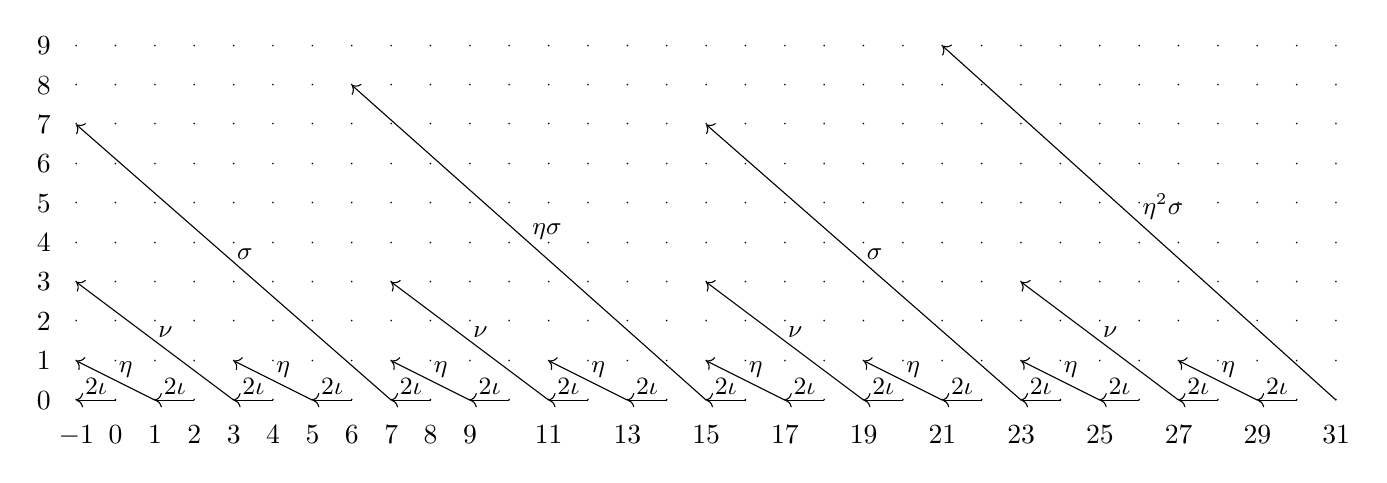
\begin{tikzpicture}[
    scale=0.5, font=\small,
    every path/.append style={->},
    every node/.append style={execute at begin node=$,execute at end node=$},
    every edge quotes/.style={auto=right,inner sep=1pt}
]
    \foreach \x in {-1,...,9,11,13,...,31}
        \node[below,font=] at (\x,-.4)  {\x};
    \foreach \y in {0,...,9}
        \node[left,font=] at (-1.4,\y) {\y};
    \foreach \x in {-1,...,31}
    \foreach \y in {0,...,9}
		\node[font=\tiny] at (\x,\y)  {\cdot};
    \foreach \x in {0,2,...,30}
		\draw (\x,0) to["2\iota" inner sep=2pt]  (\x-1,0);
    \foreach \x in {1,5,...,29}
		\draw (\x,0) to["\eta"]  (\x-2,1);
    \foreach \x in {3,11,...,27}
		\draw (\x,0) to["\nu"]  (\x-4,3);
    \foreach \x in {7,23}
		\draw (\x,0) to["\sigma"]  (\x-8,7);
    \foreach \x in {15}
		\draw (\x,0) to["\eta\sigma"]  (\x-9,8);
    \foreach \x in {31}
		\draw (\x,0) to["\eta^2\sigma"]  (\x-10,9);
\end{tikzpicture}
\end{center}

We will soon prove that there is a map of spectral sequences from the EHP sequence to the Atiyah-Hirzebruch spectral sequence constructed here and that (on the $E^1$ page) the map is induced by stabilisation. That is, ${_\text{EHP}E}^1_{pq}=\pi_{2p+1+q}(S^{2p+1})$ and ${_\text{AH}E}^1_{pq}=\pi^S_q$, and the map ${_\text{EHP}E}^1_{pq}\to{_\text{AH}E}^1_{pq}$ is just the iterated suspension map, which is an isomorphism for $q<2p$.

Since $[\iota]\in {_\text{AH}E}^1_{n-1,0}$ survives to $E^{\rho(n)}$, at which point it supports a nonzero differential, so we see that $[\iota]\in {_\text{EHP}E}^1_{n-1,0}$ must support a nonzero differential $d_r$ for some $r\leq\rho(n)$. This shows that $w_{n-1}=p\iota$ desuspends at most $\rho(n)-1$ times.

The converse holds, and could presumably be proven by constructing an explicit desuspension. That is, the first nonzero differential on $[\iota]\in {_\text{EHP}E}^1_{n-1,0}$ is exactly $d_{\rho(n)}$.
\todo{MD: What can now be said about the image of $\iota$ under the crucial differential? Is it $j(\nu(n))$ or something? I haven't thought about it.  EP: This is a good question.}
% >>>
\fi
\BoxedNote{}






\section{Matching the EHP sequence to Atiyah-Hirzebruch} % <<<
\label{MatchingTheEHPSStoAtiyahHirzebruck}
\ifx\OutputMatchingTheEHPSStoAtiyahHirzebruck\undefined\else
Last time we used a ``folk theorem'' due to Toda and Adams to the effect that the virtual bundle over $S^{\rho(n)}$ classified by $g_{\nu(n)}$ has as its Thom space the space $Cj_{\nu(n)}$ from the cofibration sequence
\begin{ctikzcd}
S^{\rho(n) - 1} \rar["j_{\nu(n)}"] & S^0 \rar & Cj_{\nu(n)}
\end{ctikzcd}
where $j_{\nu(n)}$ is the image of $g_{\nu(n)}$ under the stable version of $J$.

This is a good time to recall the definition of the $J$ homomorphism.  The action of $O(n)$ on $\Rbb^n$ restricts to a map $O(n) \times S^{n-1} \to S^{n-1}$.  If $\alpha$ represents a class in $\pi_k (O(n))$, we get
\begin{ctikzcd}
S^k \times S^{n-1} \rar{\alpha \times \id} & O(n) \times S^{n-1} \rar & S^{n-1}.
\end{ctikzcd}
Applying the Hopf construction yields a map
\begin{ctikzcd}
S^{n+k} \rar[equal] & S^k \ast S^{n-1} \rar{J\alpha} & S^n \rar[equal] & \Suspend S^{n-1},
\end{ctikzcd}
which represents a class in $\pi_{n+k}S^n$.  In proving the theorem it pays to set up the geometry very precisely.  For this purpose, define
\begin{align*}
CX & = \frac{[0, 1] \times X}{(0, x), (t, x_0)}, \\
\Suspend X & = C(X) / X.
\end{align*}
We'll study the problem in somewhat astonishing generality; our data will be a map $\varphi: A \times X \to X$ which we'll think of as a group action, although it doesn't have to be one.  The map $\varphi$ has an obvious extension $\hat \varphi: A \times CX \to CX$.  With this data we'll try to form a bundle, the first of two important constructions for today:
\begin{enumerate}
\item Associated ``bundle'' construction: This will be a ``bundle'' $p: E\varphi \to \Suspend A$ formed using $\varphi$ as the clutching map.  $E\varphi = CA \times X \coprod X / (1, a, x) \sim ax$.  The fiber is $p^{-1}(0, a) \cong X$.  Note that when $\varphi$ is a group action this construction in fact does determine an isomorphism between the fibers over the clutched coordinates, so this is genuinely a fiber bundle.  Also we can apply this construction to $\hat \varphi$, getting $E \hat \varphi$, the ``fiberwise cone on $E \varphi$;'' we'll call it $\hat E \varphi$.  Then we get
\begin{ctikzcd}
E\varphi \rar[into] & \hat E \varphi \rar & T\varphi \\
X \uar \rar[into] & CX \uar \rar & \Suspend X \uar.
\end{ctikzcd}
In our case, we had a class $g_{\nu(n)} \in \pi_{\rho(n)} BO$.  Remember though that we think of $g_{\nu(n)}$ as a class in $\pi_{\rho(n)-1}O$.  It can be thought of as a map \[S^{\rho(n)-1} \xrightarrow{g_{\nu(n)}} O(N).\]  Now $O(N)$ acts on $S^{N-1}$, so we can use this to clutch a bundle $E(g_{\nu(n)})$ over $S^{\rho(n)}$ by
\begin{ctikzcd}[column sep=0pt]
S^{\rho(n)-1} \times S^{N-1}\drar["\varphi"'] \rar{g_{\nu(n)} \times 1} &[width("$g_{\nu(n)}\times1$")+0.5em] O(N) \times S^{N-1}\dar["\mathrm{action}"] \\
 & S^{N-1}
\end{ctikzcd}
whose fiber is $S^{N-1}$.  This is the sphere bundle of the $\Rbb^N$-bundle classified by $S^{\rho(n)} \xrightarrow{g_{\nu(n)}} BO(N)$, so the Thom space we were studying last time arises from the constructions above applied to this composite, i.e., taking $A = S^{\rho(n) - 1}$ and $X = S^{N-1}$.

\item This looks very good; it looks a lot like the definition of $J$.  In order to state things correctly, we need a careful definition of the Hopf construction that matches our definition of $CX$ and $\Suspend X$.  Namely, the Hopf Construction on $\varphi$ is the quotient
\begin{ctikzcd}
A \times CX \rar{\widehat \varphi} \dar & CX \dar  \\
A \ast X \rar{J \varphi} & \Suspend X.
\end{ctikzcd}
\end{enumerate}
The theorem, then, is
\begin{thm}
There exists a homomorphism $CJ\varphi\to T\varphi$ under $\Suspend X$ making the following diagram commute:
\begin{ctikzcd}
A \ast X \rar{J \varphi} & \Suspend X \dar[into]\rar & C J \varphi \dlar["\exists"]\\
& T \varphi.
\end{ctikzcd}
\end{thm}
Note first of all that this is what we want: $\varphi$ for us is the composite
\begin{ctikzcd}
S^{\rho(n)-1} \times S^{N-1} \rar["g_{\nu(n)} \times 1"] &[-\columnsep+width("$g_{\nu(n)} \times 1$")+0.5em] O(N) \times S^{N-1} \rar & S^{N-1}
\end{ctikzcd}
and we are showing that $T\varphi$ ($ = T(g_{\nu(n)})$ from last time) = $CJ\varphi$ (= $Cj_{\nu(n)}$ from last time) relative to $\Suspend S^{N-1} = S^N$.  In fact we were interested last time in the relation between $Tg_{\nu(n)}$ and $Cj_{\nu(n)}$ stably, and we can make the fiber $S^N$ as connected as we want.  So we get a stable equivalence $Tg_{\nu(n)} \simeq Cj_{\nu(n)}$.
\begin{proof}
The hard part was parameterizing things right; now it's just a matter of drawing pictures.  In these pictures, we draw $A$ as a point and $X$ as a point.  Then we can keep track of the suspension, join, and cone coordinates.\todo{These figures need replacement.}
\begin{figure}[ht!]
\centering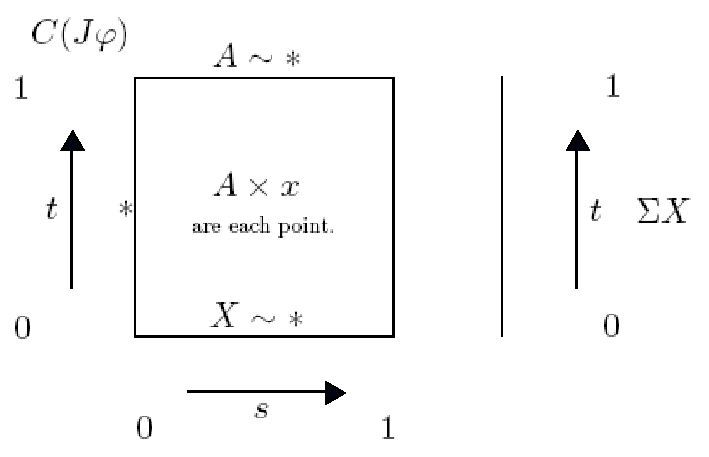
\includegraphics[width=0.3\textwidth]{figures/figure32.pdf}
\caption{\small Diagram of $CJ\varphi$.}
\end{figure}
\begin{figure}[ht!]
\centering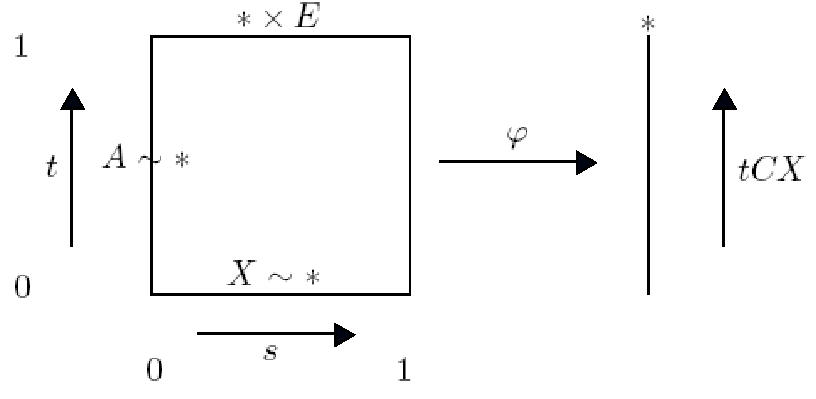
\includegraphics[width=0.3\textwidth]{figures/figure33.pdf}
\caption{\small Diagram of $T\varphi$.}
\end{figure}

So both pictures really are the same; they both look like a triangle.
\begin{figure}[ht!]
\centering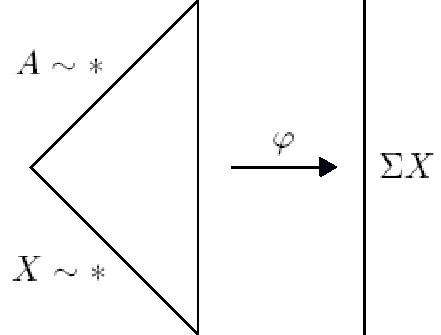
\includegraphics[width=0.2\textwidth]{figures/figure34.pdf}
\caption{\small Triangle!}
\end{figure}
And homeomorphisms with this triangle for the two spaces above are given by
\begin{align*}
f(s, a, t, x) & = \left( \frac{s - st}{1 - st}, a, st, x \right), \\
g(s, a, t, x) & = \left( s + t - st, a, \frac{t}{s + t - st}, x \right).
\end{align*}
\end{proof}

Remember how we got here: we were studying the EHP spectral sequence.  This spectral sequence has as its columns the homotopy groups of odd spheres and converged to $\pi_* QS^0 = \pi_*^S S^p$; moreover we had arranged it so that beneath a line of slope $2$, the entries in each column were the stable homotopy of spheres: \todo{INKSCAPE}  This feature suggested the question: is there a spectral sequence whose columns are the stable homotopy of spheres and a map of spectral sequences from the EHPSS to this SS such that the map is an isomorphism below the celebrated line of slope 2?

On Friday we constructed a candidate, an Atiyah-Hirzebruch spectral sequence for the attaching maps on $\RP^\infty$: $\widetilde H^*(\RP^\infty_+; \pi_*^S)$ which we hope converges to $\pi_*^S \RP^\infty_+$, whose $E^1$-term is \todo{INKSCAPE}

Sure enough, there is a spectral sequence map between these two spectral sequences which is an isomorphism below the line at $E^1$.  To see this, remember the EHP sequence: $\Loops^{n-1} S^{n-1} \to \Loops^n S^n \to \Loops^n S^{2n-1}$.  Here we looped it $(n-1)$ times as this is the form in which it went into the EHPSS.  This is a fibration, strictly if $n$ is even or localized at $2$ if $n$ is odd.  Linking these together and applying $\pi_*$ gave us the EHPSS.  On the other hand, the AHSS from Friday came from taking the cofibration sequence \[\RP^{n-2}_+ \to \RP^{n-1}_+ \to S^{n-1}_+\] and applying $\pi_*^S = \pi_* Q$.  (Recall $QX = \bigcup_k \Loops^k \Suspend^k X$.)  The sequence \[Q\RP^{n-2}_+ \to Q\RP^{n-1}_+ \to QS^{n-1}_+\] is a fibration, since $\pi_*^S$ is a homology theory and hence exact on \[\RP^{n-2}_+ \to \RP^{n-1}_+ \to S^{n-1}_+.\]  Next, note that we have \[S^{n-1}_+ \xrightarrow{e^n} \Loops^n S^{2n-1}_+ \xrightarrow{e^{\infty-n}} QS^{n-1}_+,\] and $e^{\infty-n}$ is an isomorphism on $\pi_*$ for $* < n$.

\begin{thm}
There are maps $s_n$ (``Snaith maps'' or ``Hopf-James'' maps\footnote{Oh dear.}) with
\begin{ctikzcd}
\Loops^{n-1} S^{n-1} \dar["s_{n-1}"]\rar & \Loops^n S^n \dar["s_{n}"]\rar & \Loops^n S^{2n-1} \dar["e^{\infty-n}"]\\
Q \RP^{n-2}_+ \rar & Q\RP^{n-1}_+ \rar & QS^{n-1}_+.
\end{ctikzcd}
\end{thm}
So this theorem does it.  This is a wonderful theorem; we'll try to prove it.  It was probably first proved by Nick Kuhn, although the maps are constructed by Smith.  Before we go on though, we should note two corollaries which answer an old question we've been trying to answer for a long time now.
\begin{cor}
In the portion of these sequences
\begin{cjointikzcd}[intertext,diagram sep=large]
\diagram
    \pi_{n-1} \Loops^n S^{2n-1} \dar["e^{\infty-n}"]\rar["p"] & \pi_{n-2} \Loops^{n-1} S^{n-1}\dar["s_{n+1}"] \\
    \pi_{n-1}^S S^{n-1} \rar & \pi_{n-2}^S \RP^{n-2}_+
%
\diagram \intertext{we have}
%
\diagram
    \iota \dar[mapsto] \rar[mapsto,"p"] & w_{n-1} \dar[mapsto]\\
    \iota \rar[mapsto] & \pi,
\end{cjointikzcd}
where $\pi$ is the stable homotopy class of the attaching map for the top cell in $\RP^{n-1}$ as before.
\end{cor}
\begin{proof}
The top row we've known for a while; the left leg is obvious.  The bottom row is almost as obvious; we'll have the Barratt-Puppe sequence
\begin{ctikzcd}
S^{n-1} \rar & \RP^{n-2} \rar &  \RP^{n-1} = C\pi \rar &  S^{n-1} \rar["\Suspend\pi"] & \RP^{n-2}
\end{ctikzcd}
in which the middle two maps are the cofibration on which the maps above were defined.
\end{proof}
Well, we have already deduced what happens to $\pi$ in the AHSS: the differentials on the various $\pi$ hit elements in the image of the $J$-homomorphism.
\begin{thm}
So $w_{n-1}$ desuspends to an element in $\pi_{2n-\rho(n)-2} S^{n-\rho(n)}$ and no further.
\end{thm}

% >>>
\fi
\BoxedNote{}







\section{The space of little cubes} % <<<
\label{TheSpaceOfLittleCubes}
\ifx\OutputTheSpaceOfLittleCubes\undefined\else
Today we'll examine where the Snaith maps come from, but you're going to have to believe some things.  Some references for this include May's book~\cite{May}, Cohen's paper~\cite{Cohen}, and Kuhn's paper~\cite{Kuhn}.  Remember, we're trying to construct maps
\begin{ctikzcd}
\Loops^n S^0 \rar["s_n"] & Q\RP^{n-1}.
\end{ctikzcd}
Because constructing maps out of loop spaces is hard, we'd like a tractable model for $\Loops^n S^n$.  Fortunately, there are some hints as to how to proceed.

\begin{figure}[ht!]
\centering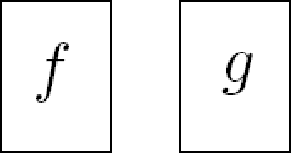
\includegraphics[width=0.2\textwidth]{figures/figure35-1.pdf}\;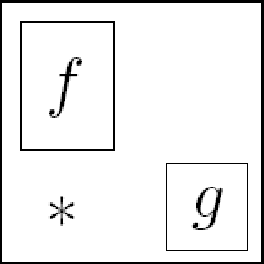
\includegraphics[width=0.2\textwidth]{figures/figure35-2.pdf}\;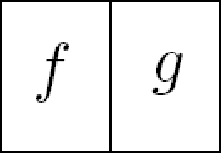
\includegraphics[width=0.2\textwidth]{figures/figure35-3.pdf}\;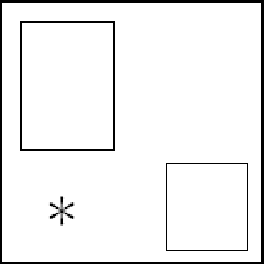
\includegraphics[width=0.2\textwidth]{figures/figure35-4.pdf}
\caption{\small $\Loops^2 X$ and the little cubes operad.}
\end{figure}
First, we do have the map $\Loops^2 X \times \Loops^2 X \to \Loops^2 X$ giving the $H$-space structure; if we represent $f \in \Loops^2 X$ and $g \in \Loops^2 X$ by the leftmost pair of boxes where the edges go to the basepoint, then their product could be represented by the second leftmost diagram, for example.  Of course, the usual representative is the second rightmost, but you have to fiddle with this any way, for example to show the product is associative or commutative up to homotopy.\todo{These figures could use repair.}  This motivates us to study spaces of rectangles.  For example, the rightmost diagram is a point in $C_2(2)$ (two rectanges in $I^2$); in general, the space $C_k(n)$ will be
\[
C_k(n) = \{ \hbox{space of $k$ disjoint parallel $n$-rectangles in $I^n$} \}
,\]
so what you're really describing is the space of embeddings $\coprod_k I^n \into I^n$.  This is called the space of ``little cubes.''  This space parameterizes the multiplication in $\Loops^n X$; namely for each $k$ we have a map $C_k(n) \times (\Loops^n X)^k \to \Loops^n X$. These piece together to give $\coprod_{k \ge 1} C_k(n) \times (\Loops^n X)^k \to \Loops^n X$.

To model the multiplicative structure you have to make some identifications:
\begin{enumerate}
\item The constant loop obliterates a cube; e.g.:
\begin{center}
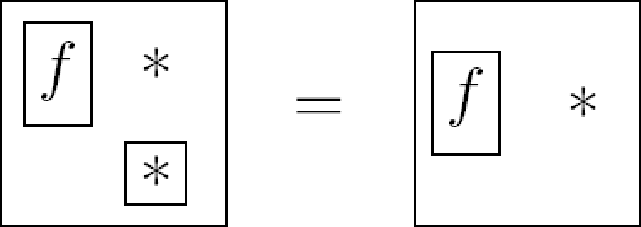
\includegraphics[width=0.2\textwidth]{figures/figure36.pdf}
\end{center}
\item The symmetric group $\Sigma_k$ acts diagonally on $C_k(n) \times (\Loops^n X)^k$, and the map is equivariant with respect to this action.
\end{enumerate}

Now if $X = \Suspend^n A$ then we have the map $\alpha: A \to \Loops^n \Sigma^n A=\Loops^n X$, and get
\begin{ctikzcd}[row sep=small]
\coprod_{k \ge 1} C_k(n) \times_{\Sigma_k} (\Loops^n X)^k / \sim \rar & \Loops^n \Suspend^n A \\
\coprod_{k \ge 1} C_k(n) \times_{\Sigma_k} A^k / \sim \uar,
\end{ctikzcd}
with the bottom $\sim$ meaning the identification in 1) above, which we won't mark down from now on.

\begin{thm}[May]
If $A$ is path-connected, this composite is a weak equivalence.
\end{thm}
This is the basic theorem in the theory of iterated loop spaces.  Note that it bears some resemblance to James' theorem.

Now you can replace each cube with its center; obviously the size of the cube doesn't affect homotopy properties.  So we get a $\Sigma_k$-equivariant equivalence
\begin{ctikzcd}
C_k(n) \rar["\simeq", "\Sigma_k"'] & F_k \Rbb^n,
\end{ctikzcd}
where $F_k(W)$ is defined to be the space of $k$-tuples in $W$ with no repeated elements.  So we have
\begin{ctikzcd}
\coprod_{k \ge 1} F_k \Rbb^n \times_{\Sigma_k} A^k / \sim & \lar["\simeq"'] \coprod_{k \ge 1} C_k(n) \times_{\Sigma_k} A^k / \sim \rar & \Loops^n \Suspend^n A.
\end{ctikzcd}
What's going on?  We're choosing $k$ many points, and rather than ordering we're labeling them with a point of $A$.  It can be constructive to think of the label as a sort of ``charge''; if the charge is zero (i.e., the point is labeled by the basepoint), we're ignoring it.  Call this space $C(\Rbb^n, A)$, following Fred Cohen's notation.

This is a pretty simple model, and we ought to be able to understand it.  Let's relate it to the James construction: so let $n = 1$.  In this case, $F_k(\Rbb^1)$ is equivalent $\Sigma_k$-equivariantly to $\{t_1 < \cdots < t_k\} \times \Sigma_k$.  In this case the God-given ordering on $\Rbb^1$ tells us the unique permutation to bring a collection of poiints into standard order.  So
\begin{ctikzcd}
C(\Rbb, A) \drar["\simeq"']\rar[equal] & \coprod_k \{t_1 < \cdots < t_k\} \times A_k / \sim \dar["\simeq"]\\
 & \coprod A^k / \sim,
\end{ctikzcd}
where $\coprod A^k / \sim$ is the James construction $J(A)$, the ``free monoid'' on $A$.  So $C(\Rbb^n, A)$ really is a generalization of the James construction.

In order to study $C(\Rbb^n, A)$, look at the obvious filtration $F(W, A)_k = \coprod_{j \le k} F_j(W) \times_{\Sigma_j} A / \sim$.  The associated quotient is
\begin{align*}
D_k(W, A) & = F_k / F_{k-1} \\
& = F_k(W) \times_{\Sigma_k} A^k / F_k(W) \times_{\Sigma_k} \{\hbox{fat wedge of} A\} \\
& = F_k(W) \times_{\Sigma_k} A^{\sprod k} / F_k(W) \times_{\Sigma_k} \ptspace.
\end{align*}
Now consider the case $A = S^q$, so that $(S^q)^{\sprod k} =_{\Sigma_k} (\Rbb^k)^q_+$, where the ``${}_+$'' denotes the $1$-point compactification.  Writing $\xi_k$ for the vector bundle $\xi_k = F_k(W) \times_{\Sigma_k} \Rbb^k$ over $B_k(W) = F_k(W) / \Sigma_k$, then $F_k / F_{k-1} = D_k(W, S^q) = T(q\xi_k \downarrow B_k(W))$.  It follows that $C(W, A)$ has a filtration whose successive quotients are Thom spaces.  In the example $W = \Rbb^n$ and $k = 2$, we have
\begin{ctikzcd}[row sep=0pt]
F_2(\Rbb^n) \rar["\cong"',"\Sigma_2"] & \Rbb^n \times (\Rbb^n \setminus \{0\}) \\
(x, y) \rar[mapsto] & \left( \frac{x + y}{2}, \frac{x - y}{2} \right),
\end{ctikzcd}
and $B_2(\Rbb^n) \cong \Rbb^{n+1} \times  \RP^{n-1}$.  We can compute $\xi_2 = 1 + L$ over $\Rbb^{n+1} \times \RP^{n-1}$, and hence \[T \xi_2 = D_2(\Rbb^2, S^q) = T(q(1+K) \downarrow \RP^{n-1}) = \Suspend^q \RP^{n+q-1}_q.\]  This is a good sign: we got a stunted projective space.

Here's another useful example: we claim that the inclusion $F_k(\Rbb^{n-1}) \into F_k(\Rbb^n)$ is null-homotopic.  A basepoint in $F_k(\Rbb^n)$ consists of a choice of $k$ distinct points, and any $k$ points in $\Rbb{n-1}$ can be smoothly moved to the fixed set of points in $\Rbb^n$ (cf., Figure \ref{ContractibilityOfFkRinfty}).
\begin{figure}%used to be [!ht]
\centering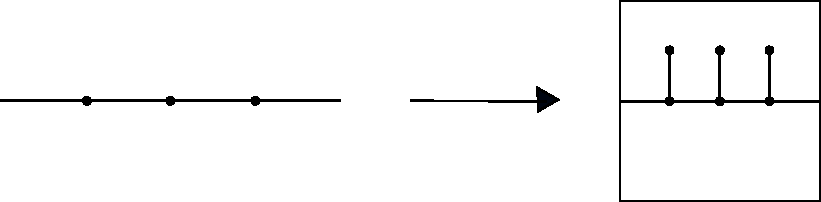
\includegraphics[width=0.35\textwidth]{figures/figure37.pdf}
\caption{\small Contractibility of $F_k \Rbb^\infty$.}\label{ContractibilityOfFkRinfty}
\end{figure}
\noindent This means that $F_k(\Rbb^\infty) = \bigcup_n F_k(\Rbb^n)$ is a contractible space with a free $\Sigma_k$-action, so it's an $E_{\Sigma_k}$ and $F_k(\Rbb^\infty) \downarrow B_k(\Rbb^\infty)$ is a universal $\Sigma_k$-bundle, and
\begin{align*}
Q(A) & = \bigcup_n \Loops^n \Suspend^n A \\
& = \bigcup_n \coprod_{k \ge 1} F_k(\Rbb^n) \times_{\Sigma_k} A^k \\
& = \coprod_{k \ge 1} E_{\Sigma_k} \times_{\Sigma_k} A^k / \sim.
\end{align*}

Let's see now how to use this to produce maps.  We're going to do this in blinding generality; namely, the map $s_k$ will be a map
\[
s_k: C(W, A) \to C(B_k(W), D_k(W, A))
\]
so a point of $C(W, A)$ is a finite subset $S \subset W$ and an assignment $f: S \to A$.  We have to take this to a finite subset $s_k S$ of points of $B_k(W)$.  The points of $B_k(W)$ are $k$-tuples in $W$, so we take for $s_k S$ the set $\{T \subseteq S : |T| = k\}$.  In addition to $s_k S$ we need an assignment $s_k f$ of points in $s_k S$ to charges in $D_k(W, A)$.  But a charge in $D_k(W, A)$ is an assignment of charges in $A$ to a $k$-element subset of $W$.  So for $T \in s_k S$, we define $s_kf(T) = f|_T$.

Now take the case $W = \Rbb^n$ and $A$ path-connected.  Then
\begin{ctikzcd}
C(W, A) \rar["\simeq","\mathrm{weak}"'] & \Loops^n \Suspend^n A \dar[into]\rar{s_k} & C(B_k(\Rbb^n), D_k(\Rbb^n, A)) \\
& C(\Rbb^N, D_k(\Rbb^n, A)) \dar[into] \\
& \Loops^N \Suspend^N D_k(\Rbb^n, A).
\end{ctikzcd}
Now when $A = S^1$ (you'd like to take $A=S^0$ but it's not connected), you get
\[
s_2: \Loops^n S^{n+1} \to \Loops^N \Suspend^N(\Suspend \RP^n)
.\]
So, looping once,
\begin{ctikzcd}
\Loops^{n+1} S^{n+1} \rar["s"] & \Loops^{N+1}\Suspend^{N+1} \RP^n \rar & Q \RP^n.
\end{ctikzcd}
There's lots of work still to be done: you have to check the compatibility of the maps and so forth.  But the model's so simple it's not hard to believe that it works.  For more information, see Kuhn's paper~\cite{Kuhn}.

% >>>
\fi
\BoxedNote{}


% -*- root: haynes-notes.tex -*-

\section{The Becker-Gottlieb transfer} % <<<
\label{TheBeckerGottliebTransfer}
\ifx\OutputTheBeckerGottliebTransfer\undefined\else
One of the advantages of a topics course is that you can change direction in midstream.  So now let's study the Adams conjecture for a while, starting with a tool by Becker and Gottlieb which enables us to get a slicker proof than the original ones of Quillen and Friedlander.  It's a construction that's of interest anyway: ``transfer.''  The basic construction is so simple that it's hard to concentrate on it long enough to appreciate how much information it contains.
\begin{enumerate}
\item Pontrjagin-Thom construction: If $X$ is a locally compact Hausdorff space and $U \subseteq X$ is an open subset, then you get a map $\pt{X} \to \pt{X} / (\pt{X} \setminus U) \simeq \pt{U}$ from the one-point compactification of $X$ to that of $U$, just by collapsing out the complement of $U$ in $\pt{X}$.  This is called the ``Pontrjagin-Thom collapse,'' and it gives a contravariance you may not have noticed before.  The construction is natural with respect to proper maps: if $f: X \to X'$ is proper, $U' \subseteq X'$, and $U = f^{-1}(U')$, then you get
\begin{ctikzcd}
\pt{X} \dar\rar["f"] & \pt{X'} \dar\\
\pt{U} \rar["f"] & \pt{U'}
\end{ctikzcd}


\item The Gysin map: Next we apply the Pontrjagin-Thom construction to the case of a smooth fibration of compact manifolds $F \to E \stackrel{p}{\to} B$.  We'd like to convert $p$ to an open embedding.  By the Whitney embedding theorem you can embed $E$ in $\Rbb^n$ for $n$ sufficiently large, and an embedding $E \into \Rbb^n$ induces an inclusion
\begin{ctikzcd}
E \dar["p"']\rar["i"] & B \times \Rbb^n \dlar\\
B
\end{ctikzcd}
Well, $i$ still isn't an open inclusion, so now consider $\nu(i)$ the normal bundle of the inclusion and get a tubular neighborhood $N$ of $E$ in $B \times \Rbb^n$.  Now the Pontrjagin-Thom collapse gives a map
\begin{ctikzcd}
\pt{(B \times \Rbb^n)} \dar[equal]\rar & N_+ \drar[equal]\rar[equal] & T(\nu(i) \downarrow E) \dar[equal]\\
T(n\varepsilon \downarrow B)\dar[equal] & & \Nbar / \partial N \\
\Suspend^n \pt{B}.
\end{ctikzcd}

Lots of Thom spaces are going to appear for a while, so perhaps we should give in and follow Atiyah's convention of writing the bundle as an exponent: $T(\nu(i) \downarrow E) = E^{\nu(i)}$.  So we have a map $B^{n\varepsilon} \to E^{\nu(i)}$.

In some sense what you're going is inverting $p$, constructing a sort of multivalued inverse.  It's instructive to think about the case that $p: E \to B$ is a finite cover.
\begin{figure}[ht!]
\centering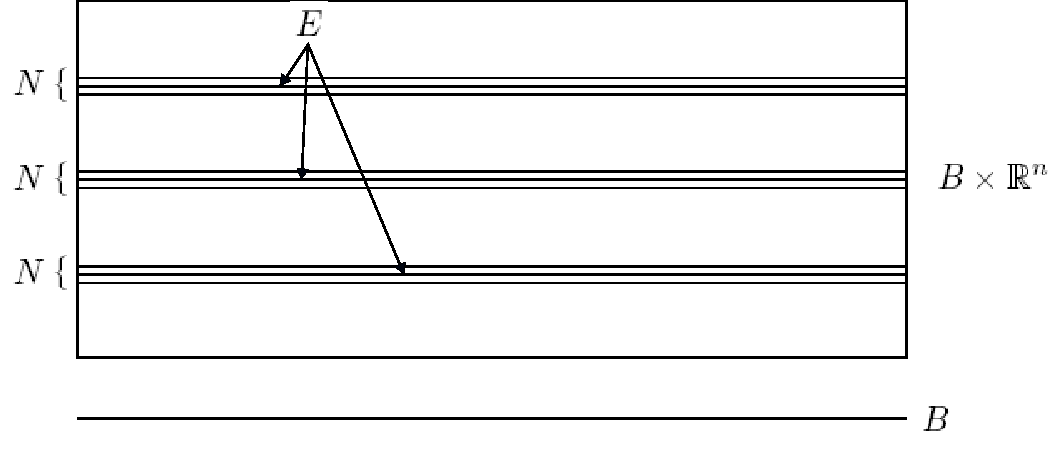
\includegraphics[width=0.4\textwidth]{figures/figure38-1.pdf}
\newline
\centering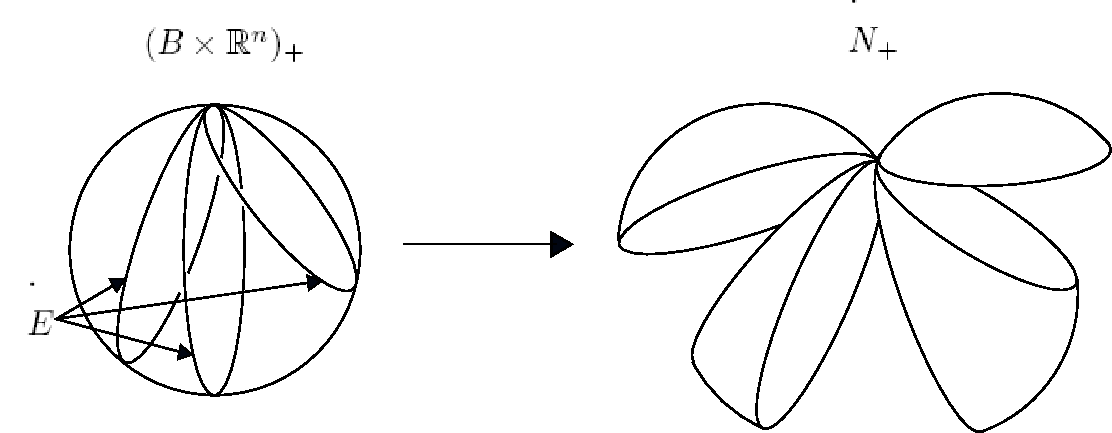
\includegraphics[width=0.4\textwidth]{figures/figure38-2.pdf}
\caption{\small Constructing the Gysin map.}
\end{figure}

The next question is: what is $\nu(i)$?  Well, $\nu(i) + \tau_E = i^*(\tau_{B \times \Rbb^n}) = p^* \tau_B + n\varepsilon_E$.  Now $\tau_E = p^* \tau_B + \tau(p)$, the ``vertical vectors'' or tangent vectors along the fiber.  So $\nu(i) + \tau(p) = n \varepsilon_E$; this is sort of a tangent bundle / normal bundle ``relative to $B$.''  So $\nu(i) = n \varepsilon - \tau(p)$, and so we get a stable map $B_+ \stackrel{p_!}{\stableto} E^{-\tau(p)}$, called the Gysin map, denoted $p_!$ for ``$p$ shriek'' or ``$p$ surprise.''  (We're also going to start writing $\stableto$ from here on out for stable maps.)

\item The Becker-Gottlieb transfer: the inclusion $\nu(i) \into n \varepsilon_E$ induces a map of Thom spaces $E^{\nu(i)} \to E^{n \varepsilon} = \Suspend^n \pt{E}$, which, together with the Gysin map,
\begin{ctikzcd}
\Suspend^n \pt{B} \rar[equal] & B^{n \varepsilon} \rar["p_!"] & E^{\nu(i)} \rar & E^{n \varepsilon} \rar[equal] & \Suspend^n \pt{E}
\end{ctikzcd}
is the Becker-Gottlieb transfer $t(p): \pt{B} \stableto E_+$, which has the virtue that it doesn't shift dimensions.
\item Euler characteristic: The Euler characteristic in this context will be defined as $\chi(p) \in \pi_S^0(B)$, an element in the stable cohomotopy of $B$.  Namely, start with the transfer $t(p): \pt{B} \stableto \pt{E}$.  Now there's a ridiculous map $\pt{E} \to S^0$ which takes the basepoint to the basepoint and pinches everything else (i.e., $E$) to the other point.  On the level of complexes, this isn't much of a map, but the claim is that stably there's a lot going on.  So the Euler characteristic is defined as $\chi(p): \pt{B} \stackrel{t(p)}{\stableto} \pt{E} \stackrel{\mathrm{pinch}}{\to} S^0 \in \pi_S^0(B)$ (i.e., unreduced stable cohomotopy).

Naturality of $\chi(p)$ follows from the naturality of $p_!$ with respect to pullbacks: if $E = f^* E'$ in TERRIBLE DIAGRAM we get $f^* \nu(i') = \nu(i)$, and $N'$ is a tubular neighborhood for $E'$ in $B' \times \Rbb^n$, we can use $f^{-1} N'$ for one of $E$ in $B \times \Rbb^n$ (we may have to choose $N'$ well, but because $B$ and $B'$ and the fiber are compact, there is no real difficulty).  Then we get the following naturality:
\begin{ctikzcd}
B^{n\epsilon} \ar[dd,"t(p)"']\drar["p_!"]\ar[rrr,"f"] & & & (B')^{n\epsilon}\ar[dd,"t(p')"]\dlar["p'_!"']\\
& E^{\nu(i)}\dlar\ar[r,"f"] & (E')^{\nu(i')}\drar\\
E^{n\epsilon} \ar[rrr,"f"] &&& (E')^{n\epsilon}
\end{ctikzcd}
The naturality of $\chi(p)$ follows by pinching out.
\end{enumerate}

We'd like to understand several things; for one, what does the Euler characteristic $\chi(p)$ have to do with the Euler characteristic in the usual sense?  Here's a start:
\begin{lem}
The following diagram commutes:
\begin{ctikzcd}
\pt{B} \dar["\Delta"']\rar[stable,"t(p)"{yshift=0.6ex}] & \pt{E} \rar["\pt{p}"] & \pt{B} \\
\pt{B} \sprod \pt{B} \dar[equal]\ar[rr,"\chi(p) \sprod 1"] & & S^0 \sprod \pt{B}\uar["\cong"'] \\
\pt{(B \times B)}
\end{ctikzcd}
\end{lem}
Before we prove the lemma, note this corollary.  Any cohomology theory has an action of stable cohomotopy: if $\alpha \in \{X, h\}$ is a class in $h^*(X)$ and $\beta \in \pi^S(X) = \{X, S\}$, then we get $\beta \cup \alpha: \Suspend X \to \Suspend X \wsum \Suspend X \stackrel{\Suspend (\alpha \wsum \beta)}{\to} \Suspend (h \wsum S) \to \Suspend h$.
\begin{cor}
If $x \in h^*(B)$, then $t(p)^* (p^* x) = \chi(p) \cup x$.
\end{cor}
\begin{proof}[Proof of the Lemma]
Consider AWFUL DIAGRAM.  Things on the left are the pullbacks of things on the right.  Then we get
\begin{ctikzcd}
B^{n\epsilon} \ar[dd,"t(p)"']\drar\ar[rrrr,"\Delta" xshift=-0.1em] & &[-2em] &[-2em] &[width("$B^{n\epsilon}$")-width("$E^{\nu(i)}\sprod B^0$")+0.6em] B^{n\epsilon}\sprod B^0\dar[dd,"t(p)\sprod 1"]\dlar\\
& E^{\nu(i)}\dlar\ar[rr,"\Delta"] && E^{\nu(i)}\sprod B^0\drar\\
E^{n\epsilon} \ar[drr,"\Suspend^n p"']\ar[rrrr,"\Delta"] &&&& E^{n\epsilon}\sprod B^0 \ar[dll,"\text{collapse $E$}"{sloped,anchor=north}]\\
&& S^N\sprod B^0
\end{ctikzcd}
\end{proof}


Now focus on $\chi(p)$ as a cohomotopy class.  We have
\begin{lem}
In $F \to E \stackrel{p}{\to} B$ the Hurewicz map $\pi^0_S B \to H^0 B$ sends $\chi(p)$ to $\chi(F)$, the usual Euler characteristic of $F$.
\end{lem}
\begin{rem}
Of course it's easier to prove the lemma if you take the right definition of $\chi(F)$.  Notice also that $\chi(p)$ in stable cohomotopy has a lot more information; when you project to cohomology you forget about $p$.
\end{rem}
\begin{proof}
Suppose $B$ is connected; pick a point $\ptspace$ in $B$.  Then $H^0(B) \stackrel{j^*}{\to} H^0 (\ptspace)$ is an isomorphism, and
\begin{ctikzcd}
F\dar["p_F"']\rar & E\dar["p"]\\
\ptspace\rar["j"] & B
\end{ctikzcd}
is a pullback, so $j^* \chi(p) = \chi(p_F)$.  So we can assume $B = \ptspace$.  The only space left is $F$.  Given an embedding $i: F \into S^n$, the Euler characteristic $\chi(p)$ is defined by $S^n \stackrel{p_!}{\to} F^{\nu(i)} \to F^{\nu(i) \oplus t(F)} \stackrel{\mathrm{pinch}}{\to} S^n$, and we must show this composite has degree $\chi(F)$.

Let $N \subset \Rbb^n$ be a tubular neighborhood for the embedded image of $F$; then $S(\nu) = \partial N$, and $\partial N$ is a codimension - 1 submanifold with an outward-pointing normal direction.  The map $F^\nu \to S^n$ is the Thom-space level of a map
\begin{ctikzcd}
\nu\dar\rar & \nu\oplus\tau \dar\rar & \Rbb^n\dar\\
F \rar & F \rar & \ptspace
\end{ctikzcd}
which on the level of sphere-bundles is a map $\gamma: \partial N \to S^{n-1}$, the Gauss map!  The degree of $\gamma$ is a standard definition of the Euler characteristic $\chi(F)$; see Milnor~\cite{Milnor} for further information.  But that's it:
\begin{ctikzcd}
S(\nu)\dar\rar["\gamma"]  & S^{n-1}\dar\\
D(\nu)\dar \rar["\gamma"] & D^n\dar\\
F^\nu \rar & S^n
\end{ctikzcd}
and the bottom pieces receive a map $S^n \to F^\nu$, the Pontrjagin-Thom collapse (which is degree 1 by construction), and the composite $S^n \to S^n$ has degree $\chi(F)$.
\end{proof}

It's worth thinking about this on the level of cohomology.  The bundle maps
\begin{ctikzcd}
\nu \dar["\zeta"']\rar{\Delta} & \{0\}\times\nu\dar{\zeta\times 1}\\
n \rar{\Delta} & \tau\times\nu
\end{ctikzcd}
induce on the level of Thom spaces
\begin{ctikzcd}
F^{\nu} \dar["\zeta"']\rar & F^0 \sprod F^\nu\dar{\zeta\times 1}\\
F^{n\varepsilon} \rar & F^{\tau}\sprod F^{\nu}
\end{ctikzcd}
If $u \in \Htwee^n(X^\xi)$ is the Thom class of $\xi$ define the Euler class $e_\xi$ as the image under pullback by $\zeta$:
\begin{ctikzcd}[row sep=0em]
\Htwee^n X^\xi \rar{\zeta^*} & \Htwee^n(X^0) \rar[equal] & \Htwee^n(X) \\
u_\xi  \rar[mapsto] & e_\xi.
\end{ctikzcd}
Then in the above square, the Thom classes go
\begin{ctikzcd}
e_\tau \cup U_\nu & \lar[mapsto] e_\tau \sprod U_\nu \\
U_{n \varepsilon} \uar[mapsto,"\zeta"]& \lar[mapsto] U_\tau \sprod U_\nu \uar[mapsto]
\end{ctikzcd}
Let $\sigma \in \Htwee^n S^n$ be a generator; think of it as the Thom class of $\Rbb^n$ over $\ptspace$.  The diagram
\begin{ctikzcd}
\nu\dar\rar & \nu\oplus\tau \dar\rar & \Rbb^n\dar\\
F \rar & F \rar{\text{pinch}} & \ptspace
\end{ctikzcd}
gives maps of Thom spaces under which $\sigma$ pulls back as
\begin{ctikzcd}[row sep=0em]
S^n\rar{c} & F^{\nu}\rar & F^{\nu\varepsilon} \rar & S^n\\
\chi(F)\cdot\sigma &\lar[mapsto] e_\tau \cup U_\nu & \lar[mapsto] U_{n\varepsilon} & \lar[mapsto] \sigma
\end{ctikzcd}
We can use classical theorems about the Euler characteristic to study our new Euler characteristic; for example, we can use Hopf's theorem to compute it in a special case.

\begin{wrapfigure}{r}{0.25\textwidth}
\centering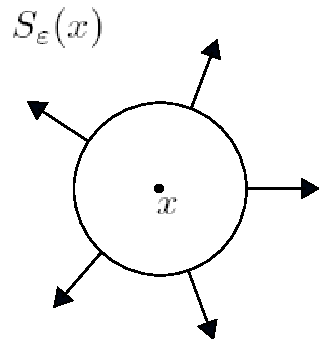
\includegraphics[width=0.25\textwidth]{figures/figure39.pdf}
\caption{\small Picture of $S_\epsilon$ about a zero at $x$.}
\end{wrapfigure}
Let $M^n$ be a compact Riemannian manifold and let $v$ be a non-degenerate vector field (i.e., $v(M)$ intersects the zero section $\zeta(M)$ of $TM$ transversally).  Then around each zero $x$ of $v$ there is a small sphere $S_\epsilon(x)$ so that $V|_{S_\epsilon(x)} \ne 0$.  Define $i_x$ to be the degree of $\frac{v}{\|v\|}|_{S_\epsilon(x)}: S^{n-1}_\epsilon \to S^{n-1} = \pm 1$.
\begin{thm}[Hopf]
$\chi(M) = \sum_{\substack{x \in M \\ v(x) = 0}} i_x$.
\end{thm}
\begin{proof}
(See Milnor~\cite{Milnor}.)
\end{proof}
For example, suppose $G$ is a compact Lie group; let $T \subset G$ be a maximal torus; let $N(T)$ be its normalizer.  Then the identity component of $N(T)$ is $T$ itself, and $N(T) / T$ is a finite discrete group, the ``Weyl group.''  The important claim is that $\chi(G / T) = |W|$ and $\chi(G / N(T)) = 1$ if $G$ is compact and connected.

To prove this, we'll come up with a vector field and use Hopf's theorem.  There is an action of $G$ on $G/T$ which restricts to an action of $T$.  In $T_eT = L(T)$ the Lie algebra of $T$ there is a vector $x$ such that $\exp x = g$, and $\exp tx$ is a path in $T$ from $e$ to $g$; let $\gamma_t$ be the induced flow on $G/T$; then $\frac{d}{dt} \gamma_t |_{t = 0}$ is a vector field on $G/T$.  Now suppose $g \in T$ is such that $\{g^n \mid n \in \Zbb\}$ is dense in $T$ (i.e., $g$ is irrational on each component of the torus; $T$ is called ``topologically cyclic''); let $v$ be the vector field on $G/T$ corresponding to this element.  A zero of $v$ is a fixed point of the action of $g$ and therefore (by continuity) a fixed point for the action of $T$.  Such a point in $G/T$ is a coset $hT$ so that $thT = hT$ for all $t \in T$, equivalently $hth^{-1} T = T$ for all $t \in T$, equivalently $h$ lies in the normalizer of $T$.  So zeroes correspond to elements of $N(T) / T = W$.  I claim all the zeroes are non-degenerate and have the same index, so $\chi(G/T) = |W|$.  Now the action of $g$ descends to $G/N(T)$ with only one fixed point, so $\chi(G/N(T)) = 1$.

Now let's talk about the transfer in $\K$-theory.  Suppose $p: E \to B$ is a finite covering.  Then the transfer is a map $t(p): B^{n \varepsilon} \to E^{n \varepsilon}$ which induces a map in $\KO$-theory $\KO(E) \to \KO(B)$.  There's an obvious thing to do here, but there's no obvious connection with the map $t(p)$: if $\xi$ over $E$ is a vector bundle, we can form a vector bundle over $B$ by taking as fiber over $b \in B$ the sum of the vector spaces over points in $E$ which cover $b$:
\begin{ctikzcd}[display math]
b \in B \rar[wavy]& \bigoplus_{p(x) = b} \xi_x = (p_* \xi)_b
\end{ctikzcd}

This is more than you might hope for; it says there's an underlying map $\mathrm{Vect}(E) \to \mathrm{Vect}(B)$.  But in fact, the two constructions are the same:
\begin{lem}[Nontrivial]\todo{Either should prove it or at least explain what's hard in the proof.}
\begin{ctikzcd}
\KO(E) \rar["t(p)^*"] & \KO(B) \\
\Vect(E) \uar[hook]\rar["p_*"] & \Vect(B)\uar[hook].
\end{ctikzcd}
\end{lem}
\begin{cor}
Let $p: E \to B$ be a finite covering and $\xi \in \KO(B)$; then if $\xi$ is stably fiber-homotopy trivial, so is $t(p)^* \xi$.
\end{cor}
\begin{rem}
Note that this isn't a trivial fact: transfer is a cohomological construction but stable fiber homotopy triviality isn't.  But it follows from the lemma: a map $S(\xi) \to S^{n-1}$ which is degree 1 on each fiber gives a map $S(p_* \xi) \to S^{n - \deg p}$ which is degree one on each fiber.
\end{rem}
\begin{rem}
The corollary can also be proved by noticing the factorization
\begin{ctikzcd}
\KOtwee(X) \dar[onto]\rar & \Sphtwee(X) \\
\Jtwee(X)\urar[into]
\end{ctikzcd}
and that $\Sphtwee = \Sphtwee^0$ is the zeroth level of a cohomology theory, using the infinite loop space theory of Boardman and Vogt.  So the transfer maps induce maps in this theory, and you can produce the result by a naturality argument.
\end{rem}

The second fact about transfer in $\K$-theory is the relation to Adams operations.  In fact, the result really concerns the interaction of Adams operations with arbitrary stable maps.
\begin{lem}
Suppose $f: \pt{x} \stableto \pt{Y}$ ; then $f^* \psi^k x - \psi^k f^* x$ has order dividing a power of $k$ (and independent of $x$).  In particular, the Adams operations are unstable.
\end{lem}
\begin{proof}
To study the problem, you have to distinguish between the stable map $f$ and an actual representative.  Let $f^*: \KO(\pt{Y}) \to \KO(\pt{X})$ denote the induced homomorphism.  Pick $n$ large enough so that there is an actual map $f: \pt{X} \sprod S^{8n} \to \pt{Y} \sprod S^{8n}$.  Then
\begin{cjointikzcd}
\diagram x\dar[mapsto]\\x\otimes\gamma^n
%
\diagram
    \KOtwee(\pt{X}) \dar{\cong}& \lar["f^*"'] \KOtwee(\pt{Y})\dar{\gamma^{\otimes n}} \\
    \KOtwee(\pt{X}\sprod S^{8n}) &  \lar["f^*"'] \KOtwee(\pt{Y}\sprod S^{8n})
\end{cjointikzcd}\todo[noline]{Check that this diagram is right.}
with $\gamma$ a generator of $\KOtwee(S^8) \cong \Zbb$.  Choosing this, you find
\begin{align*}
\psi^k(f^*(x) \otimes \gamma^n) & = \psi^k(f^*(x \otimes \gamma^n)) \\
k^{4n} \psi^k f^*(x) \otimes \gamma^n & = f^* \psi^k(x \otimes \gamma^n) \\
& = f^*(\psi^k x \otimes k^{4n} \gamma^n) \\
& = k^{4n} f^*(\psi^k x \otimes \gamma^n) \\
& = k^{4n} (f^* \psi^k x) \otimes \gamma^n.
\end{align*}
So $k^{4n}(\psi^k f^* - f^* \psi^k) = 0$, and $n$ depended only on $f$.
\end{proof}

% >>>
\fi
\BoxedNote{}

\section{The Adams conjecture} % <<<
\label{TheAdamsConjecture}
\ifx\OutputTheAdamsConjecture\undefined\else
To make greatest use of most constructions in algebraic topology, it is generally helpful to have a relative version.  This time, we'll use a relative version of the transfer map.  So, as before, let $F \to E \stackrel{p}{\to} B$ be a smooth fiber bundle with $F$ and $B$ compact; let $\xi$ over $B$ be a vector bundle, and consider
\begin{ctikzcd}
p^* \xi \dar\rar & \xi\dar \\
E \rar["p"] & B.
\end{ctikzcd}
As before, we pick an embedding $E \into \Rbb^n$ and get
\begin{ctikzcd}
E \dar["p"']\rar[into] & B \times \Rbb^n \dlar["\pr"]\rar[into]{\zeta} & n \varepsilon \oplus \xi \\
B.
\end{ctikzcd}
Now embed one step farther: $\zeta: B \times \Rbb^n \into n \varepsilon \oplus \xi$.  And we can do the collapse on the inclusion given by a tubular neighborhood for $p^* \xi$ in $n \varepsilon \oplus \xi$:
\begin{ctikzcd}
\Suspend^n B^\xi \ar[rrr,bend right=10,yshift=-0.2em, "t(p)"']\rar["p_!"] &  E^{\nu(i) \oplus p^* \xi} \rar[into] & E^{n \varepsilon \oplus p^* \xi} \rar[equal]& \Suspend^n E^{p^* \xi}
\end{ctikzcd}
The relative transfer is the corresponding stable map $t(p): B^\xi \stableto E^{p^* \xi}$.
\begin{lem}
Suppose $\chi(F) = \pm 1$.  In that case, if $\J(p^* \xi) = 0$ in $\J(E)$, then $\J(\xi) = 0$ in $\J(B)$, so $p$ is a monomorphism on $J$-theory.
\end{lem}
\begin{proof}
$\J(p^* \xi) = 0$ means that
\begin{ctikzcd}
S^d \rar & E^{p^* \xi} \rar[stable,"\exists"{yshift=0.6ex}] & S^d
\end{ctikzcd}
where the composite has degree 1 and $d$ is the dimension of $\xi$.  Then we have
\begin{ctikzcd}
S^d \rar & E^{p^* \xi} \rar[stable] & S^d \\
& B^{\xi}\uar["t(p)"'] & \lar S^d
\end{ctikzcd}
and we'd like to show the degree of this right-hand composite is $\pm 1$.  Well, choose a basepoint in $B$; then you have
\begin{ctikzcd}
d\varepsilon \ar[dd]\ar[dr]\ar[rr] & & p^*\xi\ar[dd]\ar[dr]\\
& F\ar[rr]\ar[dd] && E\ar[dd]\\
\Rbb^d \ar[rr]\ar[dr] && \xi\ar[dr]\\
& \ptspace \ar[rr,into] && B
\end{ctikzcd}
and from this you get
\begin{ctikzcd}
F^{d\varepsilon} \rar & E^{p^* \xi}  \rar[stable]& S^d \\
S^d \uar[stable] \rar & B^\xi\uar[stable].
\end{ctikzcd}
But $S^d \stableto F^{d \varepsilon}$ isn't just the inclusion of the bottom cell; in fact, we found that it was $\chi(F)$ times the inclusion of the bottom cell!  So if $\chi(F) = \pm 1$, $S^d \to B^\xi \stackrel{t(p)}{\to} E^{p^* \xi} \stableto S^d$ has degree one.

But \begin{tikzcd}S^d \rar[stable]& F^{d \varepsilon}\end{tikzcd} isn't just the inclusion of the bottom cell; in fact, we found that it was $\chi(F)$ times the inclusion of the bottom cell!  So if $\chi(F) = \pm 1$, the composition
\begin{ctikzcd}S^d \rar & B^\xi \rar["t(p)"] & E^{p^* \xi} \rar[stable]& S^d\end{ctikzcd}
has degree one.
\end{proof}

Now I'm ready to tell you what the Adams Conjecture says, although not what it means: let $B$ be a finite complex, let $\xi \in \KO(B)$, and let $k \ge 1$ an integer.  Then some power of $k$ kills $\J(\psi^k \xi - \xi)$ in $\J(B)$.

Admittedly, this is an obscure statement, but take it from me that it's important and worth proving.  We'll prove it bit by bit.
\begin{enumerate}
\item $\xi$ is a linear combination of line bundles.  If $k$ is odd then $\psi^k \xi = \xi$ so $\psi^k \xi - \xi = 0$.  If $k$ is even and $\xi$ is a line bundle (by additivity it's sufficient to consider this case), then $\psi^k \xi - \xi = 1 - \xi \in \KOtwee(B)$.  $\xi$ is classified by a map $f: B \to \RP^N$ for large enough $N$:
\begin{ctikzcd}
\xi \dar\rar & L\dar \\
B \rar["f"] & \RP^N,
\end{ctikzcd}
so $1 - \xi = f^*(1 - L)$, and $\KOtwee(\RP^N)$ is a finite 2-group generated by $(1-L)$.
\item The next case is that $\xi$ is a $2$-dimensional bundle.  Let $P$ be the associated principal bundle so that $\xi  = P \times_{O(2)} \Rbb^2$.  We described the Adams operations $\psi^k$ in terms of representations, so now we have to think a little about the representation theory of $O(2)$: what is $O(2)$?  Well, there are two parts:
\begin{ctikzcd}
S^1 \rar & SO(2) \rar[into] & O(2) \rar[yshift=0.2em] & \lar[yshift=-0.2em] \Zbb_2,
\end{ctikzcd}
where the splitting comes from choosing any reflection, say $r$ is the reflection through the $x$-axis.

So what are the representations of $O(2)$?  Let $V = \Rbb^2$ be the basic representation; then we can take exterior powers:
\begin{align*}
\lambda^0(V) & = 1, \\
\lambda^1(V) & = V, \\
\lambda^2(V) & = \det.
\end{align*}
More interestingly, we have representations $\mu_k$ given by $S^1$ acting on $\Cbb^{\otimes_\Cbb k}$ by, for $z \in S^1$, $z \cdot (w_1 \otimes \cdots \otimes w_k) = zw_1 \otimes \cdots \otimes zw_k = z^k(w_1 \otimes \cdots \otimes w_k)$, and we can extend to $O(2)$ by letting $r$ act by complex conjugation.  Note that $\mu_1 = V$.

Next we want to express the $\psi^k$s in terms of $\lambda^j$s and $\mu_k$s, so that we have some chance of being able to compute.  In order to do that, we should write down the character table for $O(2)$:
WHAT A MESS\todo{It seems like in a lot of these all caps places, we're missing things...} $\mu_k$ is the natural candidate for $\psi^k$, but it's wrong: the formula for $\psi^k$ is
\[
\psi^k = \begin{cases} \mu_k & \hbox{if $k$ is odd,} \\ \mu_k + (\lambda_0 - \lambda_2) & \hbox{if $k$ is even.} \end{cases}
\]

Now we can use the $\mu_k$s to check the Adams conjecture: $\psi^k V - V$ differs from $\mu_k V - V$ by a linear combination of line bundles with virtual dimensions $0$ (assuming $k$ is even); these are killed by a power of 2 by the above argument for the line bundle case.  if $k$ is odd, $\psi^k V - V = \mu_k V - V$.  The claim is that for some $e$, $k^e(\mu_k V - V) = 0$ in $J$.

The trick --- which is the key point in understanding the Adams conjecture --- is the map $f_k: V \to \mu_k$ given by $f_k(z) = z^k$, which is equivariant with respect to the $O(2)$ action on either side, but certainly not linear; it won't induce a map of vector bundles, but it will induce one of sphere bundles, which is degree $k$ on each fiber.  The result then follows from
\end{enumerate}
\begin{lem}[Adams' Mod $k$ Dold Lemma, Adams, $\J(X)$ I, Topology around 1965]
Let $B$ be a finite complex and let $\xi, \xi'$ be vector bundles over $B$.  Suppose $f: S(\xi) \to S(\xi')$ is degree $k$ on each fiber.  Then $k^e(\J(\xi) - \J(\xi')) = 0$ for some $e$.
\end{lem}

This is as far as Adams got; he decided it was unreasonable of others to expect him to do more.  Now you need a trick to be able to finish in a finite amount of time.

To do the general case we'll make a few reductions, namely to oriented $2n$-dimensional bundles.  A vector bundle $\xi$ over $B$ has a Stiefel-Whitney class $w_1(\xi) \in H^1(B; \Zbb_2)$ which is the obstruction to the orientability of $\xi$.  Now elements of $H^1(B; \Zbb_2)$ are in one-to-one correspondence via $w_1$ with line bundles.

Now perform the $L$ and $\Ltwee$ constructions fiberwise on the bundle $\xi$ over $B$ and you get a fiber bundle
\begin{ctikzcd}
               & \Ltwee(\xi) \dar["q"']&\lar \zeta\\
L(\Rbb^{2n})\rar & L(\xi)\dar["p"'] & \lar p^*\xi\\
               & B                &\lar\xi
\end{ctikzcd}
where $L(\Rbb^{2n})$ has $\chi = 1$ and $\zeta$ is two plane bundles.  The claim is that this wonderful formula is geometrically clear: $t(q)^* \zeta = q_* \zeta = p^* \xi$ over $B$, so in particular there is a line bundle $\lambda$ over $B$ so that $w_1(\xi \oplus \lambda) = 0$, i.e., $\xi \oplus \lambda$ is orientable.  The additivity of the Adams conjecture (plus the fact that we've already proved it for line bundles) implies that we can assume $\xi$ is an oriented, $2n$-dimensional vector bundle over $B$; moreover $B$ is compact so we can give $\xi$ a metric.

Now suppose $B$ is a $2n$-dimensional inner product space over $\Rbb$; let $F(V)$ be the space of sequence of $n$ mutually orthogonal $2$-planes in $V$.  $\Sigma_n$ acts freely on $F(V)$; let $L(V) = F(V) / \Sigma_n$.  I claim we've constructed this space before as $SO(2n)/NT$.  So $\chi(L(V)) = 1$.

Now let $\Sigma_{n-1}$ act on $F(V)$ by fixing the last element; then there is an $n$-sheeted cover $\Ltwee(V) = F(V)/\Sigma_{n-1} \stackrel{q}{\to} L(V)$.  Moreover, there is a $2$-plane bundle $\zeta$ over $\Ltwee(V)$ defined fiberwise by setting $\zeta_{(\{v_1, \ldots, v_{n-1}\}, v_n)} = v_n$.  Now from the lemma at the beginning of this lecture, it suffices to check the Adams conjecture on $p^* \xi$.  But by the formula,
\begin{align*}
\psi^k p^* \xi - p^* \xi & = \psi^k t(q)^* \zeta - t(q)^* \zeta \\
& = \psi^k t(q)^* \zeta - t(q^* \psi^k \zeta + t(q)^* \psi^k \zeta - t(q)^* \zeta \\
& = (\psi^k t(q)^* - t(q)^* \psi^k) \zeta + t(q)^*(\psi^k \zeta - \zeta).
\end{align*}
The left summand is killed by $k^e$ and the right summand is killed by $k^f$ for some $f$ by the proof of the adams conjecture for $2$-plane bundles.

% >>>
\fi
\BoxedNote{}

\section{Some summands of the stable homotopy groups of spheres} % <<<
\label{SomeSummandsOfStableHomotopyOfSpheres}
\ifx\OutputSomeSummandsOfStableHomotopyOfSpheres\undefined\else
All right, today we'll study the meaning of the Adams conjecture; in particular I'm going to tell you about the space $J$.  We've talked about the $\KO$ spectrum, representing real $\K$-theory: $\KO^*(X) = \{X, \KO\}$.  It is a sequence of spaces $\{\KO_n\}$ with maps $\alpha_n: \Suspend \KO_n \to \KO_{n+1}$, with
\begin{align*}
\KO_{8n} & = \Zbb \times BO \\
\KO_{8n-i} & = \Loops^i (\Zbb \times BO) \\
\Suspend^8 \KO_{8n} & \to \KO_{8n+8} \hbox{ is given by}
\end{align*}
\begin{ctikzcd}
S^8 \sprod (\Zbb \times BO) \dar\rar & \Zbb \times BO \\
(\Zbb \times BO) \sprod (\Zbb \times BO)\urar["\mu"].
\end{ctikzcd}
Bott periodicity says $\Zbb \times BO \stackrel{\simeq}{\to} \Loops^8(\Zbb \times BO)$.

Now $\KO(X)$ is a ring with unit; $\KOtwee^0(S^0) \cong \Zbb \ni 1$.  So there is a map of spectra $\Suspend^\infty S^0 = S \to \KO$ representing $1 \in \KOtwee(S^0)$.  One question is, how big is the image of the induced map $\pi_*^S \to \KO_*$?

Another way to ask this question is this: every spectrum has a space associated with it; in this case, we get a map $QS^0 = \Loops^\infty \Suspend^\infty S^0 \to \Zbb \times BO$ whose effect in unstable homotopy is the stable homotopy of the map above.  Viewed in this light, the answer depends on self-maps of $\Zbb \times BO$.  We have the $\psi^k$s, so we should use them.  The operation $\psi^k: \KO \to \KO$ corresponds to a map $\psi^k: \Zbb \times BO \to \Zbb \times BO$.  We know the effect of $\psi^k$ on $\pi_*$:
\[
\begin{array}{c|cc}
* & \pi_*(\Zbb \times BO) & \psi^k \\
\hline
0 & \Zbb \\
1 & \Zbb_2 \langle \eta \rangle & \eta \mapsto k \eta \\
2 & \Zbb_2 \langle \eta^2 \rangle & \eta \mapsto k^2 \eta \\
3 & 0 \\
4 & \Zbb \langle g_4 \rangle & g_4 \mapsto k^{2k} g_4 \\
5 & 0 \\
6 & 0 \\
7 & 0 \\
8 & \Zbb \langle g_8 \rangle & g_8 \mapsto k^4 g_8.
\end{array}
\]
Everything else on the table follows from periodicity.

These operations suffer from a bad defect: they're not stable.  But we've already seen how to study this problem when we were studying transfer: namely,
\begin{ctikzcd}[column sep=large]
S^8 \sprod (\Zbb \times BO) \dar["g_8\sprod 1"']\rar["k^4 \sprod \psi^k"] & S^8 \sprod (\Zbb \times BO)\dar \\
(\Zbb \times BO) \sprod (\Zbb \times BO) \dar["\mu"']\rar["\psi^k \sprod \psi^k"] & (\Zbb \times BO) \sprod (\Zbb \times BO)\dar \\
\Zbb\times BO\rar["\psi^k"] & \Zbb\times BO
\end{ctikzcd}
By adjunction, we get
\begin{ctikzcd}
\KO_0 \dar["\simeq"']\rar["k^4 \psi^k"] & \KO_0\dar["\simeq"] \\
\Loops^8 \KO_8 \rar["\psi^k"] & \Loops^8 \KO_8.
\end{ctikzcd}
The diagram measures how far $\psi^k$ is from being stable.  The fix we shall use here is to localize so that $k$ becomes a unit.

The point is, $\KO^*$ is a nice ring, so localization is easy to do: $R \subseteq \Qbb$ is flat over $\Zbb$, so we can take $\KO^*(X; R)$ to be defined as $\KO^*(X) \otimes_{\Zbb} R$; e.g., $R = \Zbb[\frac{1}{k}]$.  Then the diagram becomes
\begin{ctikzcd}[column sep=large]
\KO_0 \dar\rar{\psi^k} & \KO_0 \dar\\
\Loops^8 \KO_8 \rar["k^{-4} \Loops^8 \psi^k"{yshift=0.1em}] & \Loops^8 \KO_8 \left[ \frac{1}{k} \right],
\end{ctikzcd}
i.e., we can define a new operation $\Psi^k: \KO \to \KO[\frac{1}{k}]$ so that
\[
\Psi^k_{8n} = k^{-4n}\psi^k : \Zbb \times BO \to \Zbb \times BO \left[ \frac{1}{k} \right]
.\]
Now $\Zbb[\frac{1}{k}] \into \Zbb_{(2)}$, assuming $2 \nmid k$, so you get
\begin{ctikzcd}
\KO^* \dar\rar{\Psi^k} & \KO^* \left[ \frac{1}{k} \right]\dar \\
\KO^*_{(2)} \rar{\Psi^k} & \KO^*_{(2)},
\end{ctikzcd}
for $k$ odd.  Take the case $k = 3$ for the rest of this lecture.  But we're still not done massaging the Adams operations; we need the notion of a ``connective cover:'' if $X$ is a space, then its $n^\textup{th}$ connective cover is the space $X \langle n, \ldots, \infty \rangle \to X$, where this map is an isomorphism on $\pi_i$ for $i \ge n$ and $\pi_i X \langle n, \ldots, \infty \rangle = 0$ for $i < n$.  For example, you have
\begin{ctikzcd}
\cdots \rar & BSpin \rar & BSO \rar & BO \rar & \Zbb \times BO
\end{ctikzcd}
as a sequence of connective covers.  You can do this for spectra, in which case it's interesting to take away negative homotopy groups: $E \langle 0, \infty \rangle_n = E_n \langle n, \infty \rangle$ has no negative homotopy groups.  For example, $\KO$ has negative homotopy groups; its $0$-connective cover localized at $2$ is $\KO \langle 0,\infty \rangle_{(2)} = bo$, called ``connective real $\K$-theory.''  So
\[
\begin{array}{c|ccccccccc}
* & 0 & 1 & 2 & 3 & 4 & 5 & 6 & 7 & (8) \\
\hline
\pi_* bo & \Zbb_{(2)} & \Zbb_2 & \Zbb_2 & 0 & \Zbb_{(2)} & 0 & 0 & 0
\end{array}
\]
but now we restrict to $* > 0$.  The construction of $\Psi^k$ gives an operation on connective real $\K$-theory $\Psi^k: bo \to bo$ and we know its effect on homotopy groups ($k = 3$ in what's to follow):
\begin{ctikzcd}[column sep=0.6em]
0 & 1 & 2 & 3 & 4 & 5 & 6 & 7 & 8 & 9 & 10 & 11 & 12 & 13 & 14 & 15 & 16 \\[-1.8em]
\Zbb_{(2)}\dar["\cong"] & \Zbb_2\dar["\cong"] & \Zbb_2\dar["\cong"] & 0 & \Zbb_{(2)}\dar{\cdot9} & 0 & 0 & 0 & \Zbb_{(2)}\dar{\cdot81} & \Zbb_2 & \Zbb_2 & 0 & \Zbb_{(2)} \dar{\cdot729}& 0 & 0 & 0 & \Zbb_{(2)} \dar{\cdot9^4}\\
\Zbb_{(2)} & \Zbb_2 & \Zbb_2 & & \Zbb_2 & & & & \Zbb_{(2)} & \Zbb_2 & \Zbb_2 & & \Zbb_{(2)} & & & & \Zbb_{(2)}.
\end{ctikzcd}
Notice that $\Psi^3$ induces the identity in dimensions below $4$.  So consider the map $\Psi^3 - 1: bo \to bo$; now the map acts as $0, 0, 0, \ldots, \cdot 9 - 1, \ldots, \cdot 81 -1, \ldots$ in homotopy.  You could just take the fiber of this map, but because $\Psi^3 - 1$ induces zero in homotopy in dimensions one and two you would get copies of $\Zbb_2$ from both ends, and these are in fact unnecessary: the map $\Psi^3 - 1$ lifts to the $4$-connective cover\footnote{Why? I need to check the obstruction theory here.}
\begin{ctikzcd}
& bo \langle 4, \infty \rangle\dar \\
bo \urar[dashed]{\exists \varphi} \rar["\Psi^3 - 1"'] & bo
\end{ctikzcd}
and that brings us to the space $J$ --- or at least the spectral $j$.  Set $j$ to be the fiber of $\varphi: bo \to bo \langle 4, \infty \rangle$.  The space $J$ comes from the $0$-space:
\begin{ctikzcd}
\Zbb \times J \rar & \Zbb \times BO \rar["\varphi"] & BSpin \\
J \rar & BO\uar[into]\rar & BSpin.
\end{ctikzcd}

OK, we can figure out the homotopy of $J$ because we know about all the things that go into it.  Recall that $\nu(9^k - 1) = \nu(k) + 3$, so $9^k - 1$ is an odd multiple of $2^{\nu(k) + 3}$, or equivalently an odd multiple of $8k$.  Hence $\Psi^3 - 1$ acts either as $0$ or as multiplication by $8k$ and by a unit in $\Zbb_{(2)}$.  So we get
\begin{ctikzcd}
& 0 & 1 & 2 & 3 & 4 & 5 & 6 & 7 \\
\pi_* J & \Zbb_{(2)}\dar & \Zbb_2\dar & \Zbb_2\dar & \Zbb_8\dar & 0\dar & 0 & 0 & \Zbb_{16} \\
\pi_* bo & \Zbb_{(2)}\dar["0"] & \Zbb_2\dar["0"] & \Zbb_2\dar["0"] & 0 & \Zbb_{(2)}\dar["\cdot9-1"] & 0 & 0 & 0 \\
\pi_* bo \langle 4, \infty \rangle & 0 & 0 & 0 & 0 & \Zbb_{(2)} & 0 & 0 & 0\\[3em]
%
& 8 & 9 & 10 & 11 & 12 & 13 & 14 & 15 & 16 \\
\pi_* J & \Zbb_2\dar["0"] & \Zbb_2^2\dar & \Zbb_2 & \Zbb_8 & 0 & 0 & 0 & \Zbb_{32} & \Zbb_2 \\
\pi_* bo & \Zbb_{(2)}\dar["\cdot 81-1"] & \Zbb_2\dar["0"] & \Zbb_2\dar["0"] & 0 & \Zbb_{(2)}\dar["\cdot 9^3-1"] & 0 & 0 & 0 & \Zbb\dar["\cdot 9^4-1"] \\
\pi_* bo \langle 4, \infty \rangle & \Zbb_{(2)} & \Zbb_2 & \Zbb_2 & 0 & \Zbb_{(2)} & 0 & 0 & 0 & \Zbb.
\end{ctikzcd}

What's the point?  The point is, this has to do with homotopy groups of spheres.  You have
\begin{ctikzcd}
 & S^0\dlar\dar \\
j \rar & bo \rar["\varphi"] & bo \langle 4, \infty \rangle
\end{ctikzcd}
and the question is, how big is the image $\pi_* S^0 \to \pi_* J$?  The Adams conjecture answers this.

How?  The adams conjecture says that for some $e$, $3^e \K(\Psi^3 - 1) = 0$.  There is an inclusions $O(n) \into G_n$ ( = all degree $\pm 1$ self-maps of $S^{n-1}$) which is compatible with the inclusions $O(n) \into O(n+1)$ and $G_n \into G_{n+1}$.  So you get a map of the limits $J: O \to G = Q_{\pm} S^0$ which is an $H$-map.  So you get a map of classifying spaces $BJ: BO \to BG$.  Then the Adams conjecture implies that the composite
\begin{ctikzcd}[sep=large]
BSpin \rar & BO \rar["BJ"] & BG_{(2)} \\
 & \ular["\varphi"]BO\uar["\Psi^3-1"'] \urar["\sim *"'].
\end{ctikzcd}
This gives you a map $\alpha$ below:
\begin{ctikzcd}
J \dar["\alpha"']\rar & BO \dar\rar["\varphi"] & BSpin\dar \\
G \rar & EG \rar & BG_{(2)}.
\end{ctikzcd}
Now in fact $\alpha$ factors through the $+1$ component of $G$, $SG = Q_1 S^0$:
\begin{ctikzcd}[row sep=0pt]
    & J \dlar["\alpha"]\ar[dd,"\alpha"]\rar & BO \ar[dd]\rar & BSpin \ar[dd]\\
SG \drar\\
   & G \rar & EG \rar & BG_{(2)}.
\end{ctikzcd}
Well, this looks good, in fact it looks very good: the map $S^0 \to j$ is, after you apply $\Loops^\infty$ to it, a map $u: QS^0 \to \Loops^\infty j = \Zbb \times J$.  And in fact
\begin{ctikzcd}
J \ar[drr,"!!\simeq!!"']\rar["\alpha"] & SG \rar[into] & QS^0\dar["u"] \\
&& J
\end{ctikzcd}
So if $C$ is the fiber of $u$, then there is a homotopy equivalence $QS^0 = SG \simeq J \times C$.  Thus all of the homotopy of $J$ listed above appears as a direct summand in $\pi_* SG$, and in particular in the iamge of $S^0 \to j$.

One game you can play now is to try to get out some information on unstable homotopy.  First we'll need some names: pulling back the sequence $J \to BO \to BSpin$ once, you get $Spin \stackrel{J}{\to} J \to BO$ (where $J$ is essentially the $J$-homomorphism, in the sense that it restricts from $\alpha$).  It's time for another table:
\[
\begin{array}{cccccc}
& \pi_* Spin & \pi_* J & \pi_* BO & \hbox{New names} & \hbox{Traditional names} \\
1 & 0 & \Zbb_2 \langle \alpha_1 \rangle & \Zbb_2 & \alpha_1 & \eta \\
2 & 0 & \Zbb_2 \langle \alpha_2 \rangle & \Zbb_2 & \alpha_2 & \eta^2 \\
3 & \Zbb & \Zbb_8 \langle j_2  \rangle & 0 & \alpha_3 = 4 j_2 & j_2 = \nu \\
4 & 0 & 0 & \Zbb \\
5 & 0 & 0 & 0 \\
6 & 0 & 0 & 0 \\
7 & \Zbb & \Zbb_{16} \langle j_3 \rangle & 0 & \alpha_4 = 8j_3 & j_3 = \sigma \\
8 & \Zbb_2 & \Zbb_2 \langle j_4 \rangle & \Zbb & & j_4 = \eta \sigma \\
9 & \Zbb_2 & \Zbb_2 \langle j_6 \rangle \oplus \Zbb_2 \langle \alpha_5 \rangle & \Zbb_2 & & \mu_9, j_5 = \eta^2 \sigma \\
10 & 0 & \Zbb_2 \langle \alpha_6 \rangle & \Zbb_2 & \alpha_6 & \eta \mu_9 \\
11 & \Zbb & \Zbb_8 \langle j_6 \rangle & 0 & \alpha_7 = 4 j_6 = \eta^2 \mu_9 & j_6, \eta^2 \mu_9 \\
12 & 0 & 0 & \Zbb \\
13 & 0 & & 0 \\
14 & 0 & & 0 \\
15 & \Zbb & \Zbb_{32} \langle j_7 \rangle & 0 & \alpha_8 = 16j_7 & j_7.
\end{array}
\]

The stuff coming from $Spin$ are essentially classes in the image of the $J$-homomorphism; we had names for these already ($j_i$, see ???).  Now there's more, elements which come from $\pi_* BO$, sort of ``honorary members of the image of $J$.''  Note that $\eta = j_1$ has been demoted to an honorary member because we used $Spin$ instead of $O$.  The elements $\alpha_i$ all have order $2$; in fact, we've given names to all the elements of order $2$ that didn't have names before.  All of these really live in $\pi_*^S$!  So what we can do now is study how they behave in the EHPSS: how far they desuspend, and what their Hopf invariants are.  Or at least Mark Mahowald can.  We're in Mahowald territory in a big way now; for more information, see one of:
\ConfusedBox{ Mahowald cite{Mahowald}, Cohen cite{CohenKervaire}, Barratt, Jones, and Mahowald cite{BJM}, Selick cite{Selick}, or Feder, Gitler, and Lan cite{FGL}.}

Recall that there are ``Snaith maps'' $s_n$ that match up fibrations:
\begin{ctikzcd}
\Loops^n S^2 \dar["s_n"']\rar & \Loops^{n+1} S^{n+1} \dar["s_{n+1}"']\rar & \Loops^{n+1} S^{2n+1}\dar["e^{\infty-(n+1)}"] \\
Q \RP^{n-1} \rar & Q \RP^n \rar & Q S^n.
\end{ctikzcd}
You apply $\pi_*$ to get a map of exact couples (and so of spectral sequences):
\begin{ctikzcd}
\pi_* \Loops^n S^n \dar\rar & \pi_* \Loops^{n+1} S^{n+1} \dar\rar & \pi_* \Loops^{n+1} S^{2n+1}\dar \\
\pi_*^S \RP^{n-1} \rar & \pi_*^S \RP^n \rar & \pi_*^S S^n.
\end{ctikzcd}
$\pi_*^S$ is formidable, so now we could try to use something else to detect things; an obvious choice given the above is the spectrum $j:$ $j_n(X) = \pi_*(j \sprod X)$, so $j_* S^0 = \pi_* j = \pi_*(J \times \Zbb)$, which we know, so we might hope to be able to compute other things as well.  So by smashing with $j$, we get a map
\begin{ctikzcd}
\pi_*^S \RP^{n-1} \dar\rar & \pi_*^S \RP^n \dar\rar & \pi_*^S S^n \dar\\
j_* \RP^{n-1} \rar & j_* \RP^n \rar & j_* S^n,
\end{ctikzcd}
of exact couples (and we know that $j_* S^n$ is a summand of $\pi_*^S$!).  The bottom exact couple gives the Atiyah-Hirzebruch spectral sequence $H_*(\RP^\infty; j_*) \Rightarrow j_* \RP^\infty$.

Unfortunately, we can't do all the proofs.  Mahowald essentially does this work in the Annals paper, but he doesn't quite say it this way.

Anyway, one thing to do is to try to compute $j_* \RP^\infty$ by more direct means.  You might expect that it's huge, since $j_*$ has lots of stuff, and $\RP^\infty$ has a cell in each dimension.  But in fact it's very small; this reflects all the cancellation going on in the EHPSS --- there's lots of it.  To compute $j_* \RP^\infty$, note the fibration $S^\infty \to \RP^\infty$ induces a transfer map $\pt{\RP^\infty} \stableto \pt{S^\infty} \simeq S^0$.  There is an obvious map $\RP^\infty \to \pt{\RP^\infty}$, but be careful: on the level of spaces this \emph{isn't} a pointed map.  But on the level of spectra, you get a pointed homotopy equivalence $\Suspend^\infty \pt{X} \simeq \Suspend^\infty X \wsum \Suspend^\infty S^0$, whereas on the level of spaces you certainly don't get a pointed homotopy equivalence $\pt{X} \not\simeq X \wsum S^0$.  So anyway, you get
\begin{ctikzcd}
\RP^\infty \dar[stable]\rar[stable] & S^0 \rar & R \rar & \Suspend \RP^\infty \\
\pt{\RP^\infty}\urar[stable]
\end{ctikzcd}
where $R$ is the cofiber of $\lambda$.

\begin{wrapfigure}{r}{0.3\textwidth}
\centering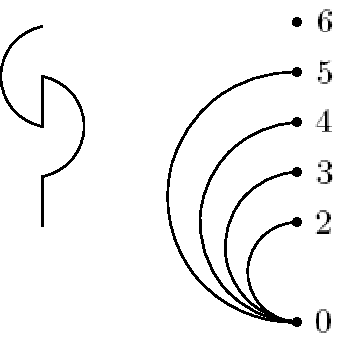
\includegraphics[width=0.2\textwidth]{figures/figure40.pdf}
\caption{\small The Steenrod action on the cohomology of $R$.}
\end{wrapfigure}
The map \begin{tikzcd}[column sep=small]\RP^\infty \rar[stable]& \pt{\RP^\infty}\end{tikzcd} is interesting because it doesn't exist unstably; constructing it involves the same game as the shifting of components we played when constructing the $J$-homomorphism.  The cohomology of $R$ has a class $x_0$ in dimension zero coming from $S^0$ and then a class $x_k$ in dimension $k \ge 2$ coming from $H^* \Suspend \RP^\infty$, and $\Sq^k x_0 = x_k$ for all $k$!  The reason for studying $R$ is that $bo_* R$ is very simple; in fact, $bo \sprod R$ is a bouquet of Eilenberg-Maclane spectra:
\[
bo \sprod R \simeq \bigvee_{k \ge 0} \Suspend^{4k} H\Zbb_{(2)},
\]
and
\[
bo \langle 4, \infty \rangle \sprod R \simeq \bigvee_{k \ge 1} \Suspend^{4k} H \Zbb_{(2)} \vee \bigvee_{k \ge 1} \Suspend^{4k+2} H\Zbb_2
.\]
And so we computed $j \sprod R$ from the sequence
\begin{ctikzcd}
j \sprod R \rar & bo \sprod R & \rar["\Psi^3 - 1"] & bo \langle 4, \infty \rangle \sprod R.
\end{ctikzcd}

It's a rational calculation; there's just not that much to do.  The result is striking: $j \sprod R$ is almost not there at all.
\[
\begin{array}{ccccc}
& j \sprod R & bo \sprod R & & bo \langle 4, \infty \rangle \sprod R \\
0 & \Zbb_{(2)} & \Zbb_{(2)} \\
1 \\
2 \\
3 \\
4 & & \Zbb_{(2)} & \stackrel{=}{\to} & \Zbb_{(2)} \\
5 & \Zbb_2 \langle \sigma_1 \rangle \\
6 & & & & \Zbb_2 \\
7 & \Zbb_2 \langle \tau_1 \rangle \\
8 & & \Zbb_{(2)} & \stackrel{\cdot 2}{\to} & \Zbb_{(2)} \\
9 & \Zbb_2 \langle \sigma_2 \rangle \\
10 & & & & \Zbb_2 \\
11 \\
12 & & \Zbb_{(2)} & \stackrel{=}{\to} & \Zbb_{(2)} \\
13 & \Zbb_2 \langle \sigma_3 \rangle \\
14 & & & & \Zbb_2 \\
15 & \Zbb_4 \langle \tau_2 \rangle \\
16 & & \Zbb_{(2)} & \stackrel{\cdot 4}{\to} & \Zbb_{(2)} \\
17 & \Zbb_2 \langle \sigma_4 \rangle.
\end{array}
\]
That's it!
\begin{align*}
j_{8k-1}(R) & = \Zbb_{2^{\nu(k)+1}} \langle \tau_k \rangle & k \ge 1, \\
j_{4k+1}(R) & = \Zbb_2 \langle \sigma_k \rangle & k \ge 1.
\end{align*}
Now we're really interested in $\RP^\infty$.
\[
\begin{array}{cccc}
& j \sprod \RP^\infty & j \sprod S^0 & j \sprod R \\
0 & \Zbb & \Zbb & \Zbb_{(2)} \\
1 & \Zbb_2 & \Zbb_2 \langle \alpha_1 \rangle \\
2 & \Zbb_2 & \Zbb_2 \langle \alpha_2 \rangle \\
3 & \Zbb_8 & \Zbb_8 \langle j_2 \rangle \\
4 & \Zbb_2 \langle \sigma_1 \rangle \\
5 & 0 & & \Zbb_2 \langle \sigma_1 \rangle \\
6 & \Zbb_2 \langle \tau_1 \rangle \\
7 & \Zbb_{16} & \Zbb_{16} \langle j_3 \rangle & \Zbb_2 \langle \tau_1 \rangle \\
8 & \Zbb_2 \oplus (\Zbb_2 \langle \sigma_2 \rangle) & \Zbb_2 \langle j_4 \rangle \\
9 & \Zbb_2 \oplus \Zbb_2 & \Zbb_2 \oplus \Zbb_2 & \Zbb_2 \langle \sigma_2 \rangle \\
10 & \Zbb_2 & \Zbb_2 \\
11 & \Zbb_8 & \Zbb_8 \langle j_6 \rangle \\
12 & \Zbb_2 \langle \sigma_3 \rangle & 0 \\
13 & 0 & 0 & \Zbb_2 \langle \sigma_3 \rangle \\
14 & \Zbb_2 \langle \tau_2 \rangle  & 0 \\
15 & \Zbb_{32} & \Zbb_{32} \langle j_7 \rangle & \Zbb_4 \langle \tau_2 \rangle \\
16 & \Zbb_2 \oplus \Zbb_2 \langle \sigma_4 \rangle & \Zbb_2 \langle j_8 \rangle.
\end{array}
\]
AND AN UNREADABLE ROW.  Various things could happen, but in fact nothing else does:
\[
j_* \RP^\infty \cong j_* \oplus \langle t_k, \sigma_k \rangle.
\]
So now we've computed the $E^2$-term and the ``abutment'' of the Atiyah-Hirzebruch spectral sequence $H^*(\RP^\infty; j_*) \Rightarrow j_* \RP^\infty$.  A picture is attached of what the filtration looks like; we've really reached the outer limits of human comprehension here.  Note that each of the dots is a $\Zbb_2$, so a non-zero differential connecting two dots is death to both of them.  So you get to $E^\infty$ from $E^2$ pretty quickly, and you can see a good deal of $E^\infty$ in this picture.

Remember what we had: there were three exact couples
\begin{ctikzcd}
\pi_* \Loops^n S^n \dar\rar & \pi_* \Loops^{n+1} S^{n+1} \dar\rar & \pi_* \Loops^{n+1} S^{2n+1} \dar \\
\pi_*^S \RP^{n-1} \dar\rar & \pi_*^S \RP^n \dar\rar & \pi_*^S S^n \dar\\
j_* \RP^{n-1} \rar & j_* \RP^n \rar & j_* S^n,
\end{ctikzcd}
and the last spectral sequence can be written out completely; it's the chart.  Today we'll talk about two problems: first, given a class $v \in j_* \RP^\infty$, where can be find a representative, which we will denote $H(v)$, in $j_*$? and secondly, how do classes in $j_* \RP^\infty$ pull back to $\pi_*^S \RP^\infty$, or even better, to the EHP sequence?
\begin{ctikzcd}
S^k \ar[ddr,end anchor=north west]\drar[end anchor=north west]\rar & j \sprod \RP^\infty \\
& |[inner xsep=0pt]|j \sprod \RP^3\uar\dar \\
& |[inner xsep=0pt]|j \sprod S^3.
\end{ctikzcd}
Recall $j_* \RP^\infty = j_* \oplus \langle \tau_k, \sigma_k$, and $j_*$ contained elements $\alpha_k$ of order $2$ and elements $j_k$.  Recall also that $\alpha_k$ were often not generators; for example, $\alpha_3 = 4j_2$.  So we introduce the notation that $\alpha_{k/i}$ is an element such that $2^{i-1} \alpha_{k/i} = \alpha_k$.  For example, $\alpha_4 = 8 \sigma$, so $\alpha_{4/2} = 4 \sigma$, $\alpha_{4/3} = 2\sigma$, $\alpha_{4/4} = \sigma$, and $\alpha_{4/1} = \alpha_4$.  With this notation we can get all the classes in the image of $J$ except $j_{4k}, j_{4k+1} \in \pi_{8k} J, \pi_{8k+1} J$.  Then the representatives of $j^* \RP^\infty$ in this spectral sequence are found as follows:
\begin{align*}
H(\alpha_{k/i}) & = \alpha_{k-i} \\
H(j_{4k+1i}) & = j_{4k+i-1}, & i = 0, 1 \\
H(\sigma_k) & = \nu = j_2 \in \pi_3(J) \\
H(2^i \tau_k) & = j_{i+1}, & i \le \nu(k).
\end{align*}
Some patterns you will observe when you compare this with the picture:
\begin{enumerate}
\item Elements in the image of $J$ are born as early as possible, so they are concentrated on the left of the table.
\item $\sigma_k$s are born as \emph{late} as possible, so they occur to the \emph{right} on their total degree lines.
\item $\tau_k$s are born as late as possible, subject to the requirement that $2^i \tau_k$ are born as late as possible too.
\end{enumerate}
The next question we posed for ourselves was: how does this picture pull back to the EHP sequence and $\pi_*^S = \pi_* QS^0$?  Mahowald's answer is
\begin{thm}(Mahowald)
The image of $\pi_*^S = \pi_* QS^0 \to \pi_*^S \RP^\infty \to j_* \RP^\infty$ contains $\Jtwee_*$, $\sigma_{2^k}$ for $k \ge 1$, and may contain $2^k \tau_k, k \ge 0$ (coming from Kervaire invariant classes; we know that $\theta_2, \ldots, \theta_5$ do exist with $\theta_{k+2} \in \pi^S_{8 \cdot 2^k-2}$), and \emph{nothing else}!
\end{thm}
What does this tell us about our picture?  For elements in the image of $J$, the EHP spectral sequence looks the same as our chart.  Elements in the image $\pi_* J \to \pi_*^S$ are born on the expected spheres (they can't be born earlier than they are here, and Mahowald constructed such elements in the EHP spectral sequence in the right dimensions in his paper) and their Hopf invariants have the right image in $j_* S^n$ under the map of spectral sequences.  In fact, a great deal of the information from various parts of the course can be discerned in the picture.  For example, Hopf invariant 1 is present: if you project
\begin{ctikzcd}
\pi_*^S S^0 \rar & \pi_*^S \RP^\infty \rar & j_* \RP^\infty \rar & j_*  \RP^\infty_n
\end{ctikzcd}
with $n$ odd, then $\pi_*^S S^0 \to j_* \RP^\infty_n = \Zbb_2$ is the Hopf invariant.  So you have an element of Hopf invariant 1 if you have a survivor in the bottom row.

The issue of the desuspension of $w_n$ (and so of vector fields on spheres) became a picture of differentials off classes in the bottom row of the Atiyah-Hirzebruch spectral sequence for $\pi_*^S \RP^\infty$; the desuspension of $w_n$ is represented by the end of the differential.

The desuspension of $w_n$s brings us to the Kervaire Invariant classes.  Notice in the picture at the $(7, 7)$ position the differential coming in above from the bottom row: INKSCAPE  What you would hope is that $\theta_3 = \frac{1}{2}$ times the desuspension of $w_15$.  So that's part of the wish list for Kervaire invariant classes:
\begin{itemize}
\item $\theta_k \in \pi^S_{2^{k+1}-2}$
\item born on $S^{2^{k+1} - 1 - |j_k|}$
\item Hopf invariant of $j_k$ (or at least having some image in $j_*$ as $j_k$
\item order 2 (since in $j_* \RP^\infty$, $2^k \tau_{2^k}$ has order 2)
\item $\theta_k$ halves a maximal desuspension of $w_{2^{k+1}-1}$
\item no further division by $2$ is possible, because in $j_* \RP^\infty$ further divisors exist, but these are not in the image of $\pi_*^S$
\item detected on the Adams $2$-line.
\end{itemize}
Other things have been done: you could investigate further how the classes that are in $\pi_*^S$ behave in the EHP sequence; for example, you could try to compute $p(j_k)$.  Mahowald's theorem tells good information about when these are nonzero.  Feder, Gittler, and Lan (cite them) have shown other classes for which $p(j_k) = 0$.  But the Kervaire Invariant classes represent a real missing case here, about which relatively little is known.
% >>>
\fi
\BoxedNote{}



\ifx\OutputTheBibliography\undefined\else
\begin{thebibliography}{Hatcher}
\bibitem{Adams} J.\ Frank Adams.  \emph{Stable Homotopy and Generalised Homology}.  University of Chicago Press, 1974.
\bibitem{Atiyah} Michael Atiyah.  \emph{Thom Complexes}.  Proceedings of the London Mathematical Society, 1960.
\bibitem{BullettMacDonald} Shaun Bullett, Ian MacDonald.  \emph{On the Adem Relations}.  Topology, 1982.
\bibitem{Cohen} F.\ R.\ Cohen, \emph{Unstable Decomposition of $\Loops^2 \Suspend^2 X$}.  Math.\ Zeit, 1983.
\bibitem{James} Joan James. \emph{The Topology of Stiefel Manifolds}.  London Mathematical Society, 1976.
\bibitem{Kuhn} Nick Kuhn, \emph{The Geometry of James-Hopf Maps}.  Pacific J., 1982.
\bibitem{May} J.\ P.\ May, \emph{Geometry of Iterated Loop Spaces}.
\bibitem{Milnor} John Milnor, \emph{Topology from a Differentiable Viewpoint.}
\bibitem{Whitehead} George Whitehead.  \emph{Homotopy theory}.  MIT Press, 1971.
\end{thebibliography}
\fi

\end{document}

